% AU template last modified by AU: 2010 Jul 02
% SH modifications for Markdown made in September 2018

\documentclass[12pt,econ]{sources/authesis}
\usepackage{natbib}  % natbib citation style
% The next two lines break hyphens in the bibliography
\usepackage{url} 
\def\UrlBreaks{\do\/\do-}
% The following packages are for the LaTeX generated graph
\usepackage{tikz}
\usepackage{pdflscape}
\newcommand{\blandscape}{\begin{landscape}} % for the framing landscape tables
\newcommand{\elandscape}{\end{landscape}}
\usepackage{threeparttable}
\def\tightlist{}
% The next three lines put the page number non-rotated and to the top right of the page
\def\fillandplacepagenumber{%
 \par\pagestyle{empty}%
     \vspace{-15.5cm}\hspace{15.8cm}\normalsize{\thepage}}
\usepackage{caption}
\usepackage[hidelinks]{hyperref}
\usepackage{float} % to float tables
\usepackage{longtable} % for tables that are longer than one page
\usepackage{booktabs} % for stuff like \bottomrule in tables
\usepackage{adjustbox} % for \resizebox for tables
\usepackage{dcolumn} % to align on the decimal point of numbers in table columns
\usepackage{bm} % to make math symbols bold with \bm{}
\usepackage{changepage} % for \adjustwidth
\usepackage{amsfonts} % for math symbol "mathfrak"

% next 11 lines to create math symbol "reallywidehat"
\usepackage{scalerel,stackengine}
\stackMath
\newcommand\reallywidehat[1]{%
\savestack{\tmpbox}{\stretchto{%
  \scaleto{%
    \scalerel*[\widthof{\ensuremath{#1}}]{\kern-.6pt\bigwedge\kern-.6pt}%
    {\rule[-\textheight/2]{1ex}{\textheight}}%WIDTH-LIMITED BIG WEDGE
  }{\textheight}% 
}{0.5ex}}%
\stackon[1pt]{#1}{\tmpbox}%
}
\def\changemargin#1#2{\list{}{\rightmargin#2\leftmargin#1}\item[]}
\let\endchangemargin=\endlist 


%%-------------------------------------------------
%% For flowchart(s)
%%-------------------------------------------------

\usetikzlibrary{shapes,arrows,positioning}

% Define block
\tikzstyle{block} = [rectangle, draw, fill=blue!20, text width=1cm, text centered, rounded corners, minimum height=3em]

% Define another block
\tikzstyle{block2} = [rectangle, draw, fill=blue!20, text width=3cm, text centered, rounded corners, minimum height=2em]

% Define another block
\tikzstyle{block2r} = [rectangle, draw, fill=red!20, text width=3cm, text centered, rounded corners, minimum height=2em]

% Define another block
\tikzstyle{block2rw} = [rectangle, draw, fill=red!20, text width=7cm, text centered, rounded corners, minimum height=2em]

% Define yet another block
\tikzstyle{block3} = [rectangle, draw, fill=blue!20, text width=2cm, text centered, rounded corners, minimum height=3em]

% And another block
\tikzstyle{block4} = [rectangle, draw, text width=3cm, text centered, rounded corners, minimum height=3em]

% Define cloud
\tikzstyle{cloud} = [draw, ellipse, fill=red!20, node distance=1cm, minimum height=3em]

% Define another cloud
\tikzstyle{cloud2} = [draw, ellipse, node distance=1cm, minimum height=3em]

% Define another cloud
\tikzstyle{cloud3} = [draw, ellipse, fill=red!20, node distance=1cm, minimum height=2em]

% Define line
\tikzstyle{line} = [draw, -latex', node distance = 0.1cm, auto]


% 
% FIGURES
%
\usepackage{graphicx}
% SH: The following generates all images so they have a width \maxwidth. This means that they will get their normal width if they fit onto the page, but are scaled down if they would overflow the margins:
\makeatletter
\def\maxwidth{\ifdim\Gin@nat@width>\linewidth\linewidth
\else\Gin@nat@width\fi}
\makeatother
\let\Oldincludegraphics\includegraphics
\renewcommand{\includegraphics}[1]{\Oldincludegraphics[width=\maxwidth]{#1}}
% SH: The following is repeated from the .cls file to make it appear in Markdown. The commands set the figure float, count etc.
\makeatletter
\def\fps@figure{ht} 
\def\ftype@figure{1}
\def\ext@figure{lof}
\def\fnum@figure{\figurename~\thefigure}
\def\figure{\@float{figure}}
\let\endfigure\end@float
\@namedef{figure*}{\@dblfloat{figure}}
\@namedef{endfigure*}{\end@dblfloat}
\makeatother
% SH: The following is repeated from the .cls file to make it appear in Markdown. The commands set the captions and also make the lof and lot double-spaced (unless it extends to more than one line, in which case it's single-spaced)
\makeatletter
\def\caption{\refstepcounter\@captype \@dblarg{\@caption\@captype}}
\long\def\@caption#1[#2]#3{%
  \par \par
  \addcontentsline{\csname ext@#1\endcsname}{#1}%
    {\protect\numberline{\csname the#1\endcsname.}{\ignorespaces #2}}%
  \addtocontents{\csname ext@#1\endcsname}{\protect\addvspace{10\p@}}%
  \begingroup
    \@parboxrestore
    \if@minipage
      \@setminipage
    \fi
    \normalsize
    \itshape % SH: Added \itshape myself for aesthetics -- to distinguish figure caps from text
    \@makecaption{\csname fnum@#1\endcsname}{\ignorespaces #3}\par
  \endgroup}
\makeatother
% end SH



% Declarations for Front Matter
%
% IMPORTANT: IF A TITLE OR SUBTITLE EXCEEDS MORE THAN ONE LINE,
%            THERE SHOULD ONLY BE  48 CHARACTERS PER LINE.
%
% The dissertation title must be capitalized for AU-CAS

\title{WHAT PEOPLE THINK: ADVANCES IN PUBLIC OPINION MEASUREMENT USING ORDINAL VARIABLES}
\author{Simon Heuberger}
\degreeyear{2021}
\degree{Doctor of Philosophy}
\chair{Professor Jeff Gill}
\secondreader{Professor Ryan T. Moore}
\thirdreader{Professor Elizabeth Suhay}
\fourthreader{Professor R. Michael Alvarez}
\fifthreader{Professor Elizabeth Malloy}
\degreefield{Political Science}

\begin{document}

\maketitle

\maketitle

% The following command makes the copyright page

\copyrightpage

% The frontmatter environment uses roman lower case page numbering. The
% abstract, acknowledgements, table of contents, list of figures, and
% list of tables are a part of this environment.
\begin{frontmatter}

% The Guide requires one numbered abstract page.
% The 'abstractn' macro generates a numbered abstract page.
% Do NOT use the 'abstract' macro, which generates an unnumbered, abstract page.
% (NOTE: The Guide no longer requires two abstract pages, one numbered, one without numbers.)

\abstractn{Surveys are a central part of political science. Without surveys, we would not know what people think about political issues. Survey experiments also enable us to test how people react to given treatments. Surveys and survey experiments are only as good as the analytical techniques we as researchers use, though. This applies particularly to how we use and measure variables. For ordinal variables, some of our current measurements and techniques are insufficient. Ordinal variables consist of ordered categories where the spacing between each category is uneven and not known. One example is education, one of the most important predictors of political behavior. The distances between education categories such as ``Elementary School'', ``Some High School'', and ``High School Graduate'' are not evenly spread. Current practice nonetheless often does not take this information into account. This could misrepresent the data and potentially distort results. My dissertation develops two methods to address this and applies them in original survey research. Chapter \ref{ordblock} develops a new method to improve the use of ordinal variables in blocking in survey experiments. Preliminary evidence suggests that the re-estimation of ordinal variable categories with an ordered probit approach might matter, but the results are mixed. Chapter \ref{ordmiss} develops a new method to treat missing survey data with ordinal variables. The results show that the method performs worse than existing software, despite expectations to the contrary. Chapter \ref{framing} applies both methods in an online survey experiment that tests morality and self-interest in political framing. The results confirm the negative findings from the previous chapters but also show tentative evidence for the importance of morality in issue-opposing frames.}

%This is an abstractn.  There are page numbers.
%The \emph{Guide} says an abstract should not exceed 350 words.
%(If you do exceed this,
%then under the CAS option, the first page is numbered bottom center, and %the rest are numbered top right.)


% Acknowledgements are optional. If you do not wish to include them,
% simply do not include this command in your source.

\acknowledgements{Throughout the writing of this dissertation I have received a great deal of support and assistance. First and foremost, I want to thank my supervisor and chair Jeff Gill. It is safe to say that this dissertation would not exist without him. He has been my guide in the world of political methodology and has set me on a path I would not have taken without him. In addition to his invaluable and unwavering support throughout this project, Jeff also trusted me with the replications for Political Analysis. Working for PA has provided me with contact to scholars around the world, which has opened countless doors to job opportunities. It was a pleasure and a true honor to work with Jeff all these years.\newline
I am also extremely grateful for all the other members on my committee. Ryan Moore has accompanied me on my graduate journey from the beginning as my teacher, supervisor, and committee member. He introduced me to \texttt{R} six years ago, and I have never looked back. He has been a fountain of knowledge in all things statistics and coding throughout. Without Liz Suhay, the framing chapter would be a shadow of what it has become. Her passion for emotions and clear eye for detail has been a huge support in designing the experiment and developing the questionnaire. I met Mike Alvarez through my work for PA several years ago. He has been an inspiration on replication work, and I am honored that he accepted my invitation to join the committee. Finally, Betty Malloy very kindly agreed to serve as the external reader at very short notice during tumultuous Covid times. I am extremely grateful for all their contributions and support. I consider myself very lucky to have been given the chance to work with such outstanding scholars.\newline
On a personal level, thanks are endless. To my friend Gabe: You have been a hero during the dissertation stage. I could not and would not have done this without you. When things got tough, you were there. Your \texttt{R} proficiency leaves a little to be desired but hey, no one is perfect. I missed you terribly during these Covid times and hope to see you again soon. To my friend Hauke: We have known each other for many years, and I am blessed by each one. I will never forget the emotinal and practical support you have given me all this time. I am honored to be Linus' godfather. To many, many more years of friendship to come. Lastly, to my family Angelika, Ludwig, Katherina, Kilian, Lorenz, and Michela: You guys are my everything. No more and no less. I don't know what I would do without any of you. Life is good because of you.\newline
Last but not least: Eternal gratitude for love and devotion that outshines humankind to Fendi and Muesli, the two greatest creatures on the planet, the best things I have ever done. And of course to Waldemar Burgo.}


\listoftables

\listoffigures

\tableofcontents


\end{frontmatter}

\hypertarget{intro}{%
\chapter{INTRODUCTION}\label{intro}}

News outlets, political campaigns, and survey institutes spend millions of dollars every year in the attempt to uncover what people think. The exact nature of public opinion is highly sought after information. It is not hard to see why: Public opinion is central to the functioning of democracy. It consists of the desires and wants of people. Their collective views and opinions determine who gets elected, what policies are enacted, and how society is structured. We need to know what people want, how they think, how they feel, what they support, and what they oppose because these wants and desires directly inform policy making and political decisions. We do so by conducting surveys. Surveys are a central part of public opinion. Without surveys, we would not know what people think. They collect data from a population or a sample population to gain information and insights into political issues. Surveys are ubiquitous in today's media environment. Research institutes like the Pew Research Center conduct dozens of surveys on numerous topics every year. In the run-up to the 2020 presidential election, the number of opinion polls conducted in swing states easily reached triple digits.

In political science, surveys are often used to analyze political attitudes. To establish causal effects, researchers use survey experiments. Like surveys, survey experiments collect background information on people's demographics. Unlike surveys, however, they also include attempts to uncover treatment effects on public opinion by testing one or several hypotheses. Similar to a laboratory setting, this involves exposing respondents to differing conditions in order to determine the effect of the intervention in question. In medical research, a treatment may take the form of a pill. In a survey context, a treatment can take the form of particular types of questions, different question wordings, or exposure to a particular type of content, among many others. Survey experiments are one of the most powerful methodological tools in political science. By combining experimental design that provides clear causal inference with the flexibility of the survey context as a site for attitude research, survey experiments can be used in almost any field to study almost any question.

Surveys and survey experiments are only as good as the analytical techniques we as researchers use, though. This applies particularly to how we phrase and measure the questions we ask respondents. If a question is worded confusingly, for instance with a double negative, we cannot gain much insight from it. If we provide unsuitable response options, for example in multiple choice questions, we might obtain inaccurate information. Take for instance a potential question inquiring after support for the legalization of marijuana. Say this question only offered the response choices ``Yes, I support legalization'' and ``No, I don't support legalization''. Are these good choices? Most likely not. Restricting the range of possible answers to a binary choice denies respondents the chance to voice more complex opinions. Some people might support legalization a little bit. Others might be highly enthusiastic about it. Yet others again might rigidly oppose it, while a fourth group is ambivalent about the subject. How we word questions and how we measure responses matters. This does not end at questionnaire design. How we use the collected information for subsequent analysis is just as, if not more, important. The statistical techniques and methods we use to analyze survey and survey experiment data crucially influence the results we obtain. This applies particularly to different types of variables. While some variables are comparatively easy to wrangle, such as numerical ones, others provide a greater challenge. For one particular type, namely ordinal variables, I consider some of our current analytical techniques to be insufficient.

Ordinal variables are part of the larger framework of categorical variables. Categorical variables represent types of data which are commonly divided into three groups: nominal, interval, and ordinal. Nominal variables are categorical variables with two or more categories that are not intrinsically ordered. Examples include gender (Female, Male, Transgender etc.), race (African-American, White, Hispanic etc.), and party ID (Democrat, Republican, Independent) where the categories cannot be ordered sensibly into highest or lowest. Interval variables are ordered categorical variables with evenly spaced values. Examples include income (\$20,000, \$40,000, \$60,000, \$80,000 etc.), where the distance between \$20,000 and \$40,000 is the same as the distance between \$60,000 and \$80,000. Ordinal variables are ordered categorical variables where the spacing between values is not the same. Examples include education (Elementary School, Some High School, High School Graduate etc.) where the distance between ``Elementary School'' and ``Some High School'' is likely different than the distance between ``Some High School'' and ``High School Graduate''. Each subsequent category has quantitatively more education than the previous one, but the exact measure of the distances between the categories is not known.

Current practice often does not take ordinal variable information into account. One such technique involves turning ordinal categories into categorical indicators. Researchers here create a new binary variable for an education category, for instance ``High School Graduate''. While it removes the issue of uneven distances, this approach ignores the ordered nature contained in ordinal variables. Education categories are treated like nominal variables, i.e.~we would wrongly assume that the ordering of education categories is arbitrary. Ordinal variables are also often made numerical for analytic purposes. This is problematic because of their unevenly spaced categories. If we turn the education categories ``Elementary School'', ``Some High School'', and ``High School Graduate'' into the numerical values 1, 2, and 3, we wrongly assume that the distances between the education categories correspond to these evenly spaced values. Do the numbers 1 to 3 really represent the distances between these categories? Perhaps the true spacing between some of the categories is so narrow they should not even be separate categories at all. We cannot answer this by making an arbitrary assumption that may not be justified by the data. Important information might be lost for one of the major predictors of political opinion, which could lead to distortion (O'Brien, 1981). To truly use the ordinal nature of a variable, we need to use its inherent unevenly spaced order to make a more underlying description of the data possible (Agresti, 2010). To fill this gap, I propose an ordered probit approach that estimates an ordinal variable's underlying latent continuous structure. I use this approach to develop two methods: The first method improves the use of ordinal variables in blocking in survey experiments. The second method provides a new way to treat missing survey data with ordinal variables. I subsequently apply both methods in an online survey experiment on political framing.

Chapter \ref{ordblock} outlines the blocking method. Survey experiments depend on balance to enable causal estimates. In order to identify potential causal effects, all treatment groups in a survey experiment need to be balanced on the potential outcomes. We get there by making all treatment groups look the same in terms of covariates. While this can be achieved with randomization, this typically leads to problems for small samples. Blocking, i.e.~arranging participants in groups that are equal in terms of participants' covariates and using random allocation within these groups, can alleviate such worries. I use an ordered probit approach to estimate an assumed underlying latent continuous structure underneath ordinal variables, which results in a new set of data-driven variable categories that can then be used for blocking. This avoids arbitrary numerical conversion and fully utilizes the ordinal information provided in the unevenly spaced variable categories. I test this method by blocking external survey data, conducting variance tests, and running a placebo regression. Findings are mixed, with some results supporting the notion that the re-estimation of ordinal variable categories with an ordered probit approach matters and others negating it.

Chapter \ref{ordmiss} describes a new method to treat missing survey data with ordinal variables. Missing data are ubiquitous in survey research (Allison, 2002; Raghunathan, 2016). This poses a big problem for researchers because data can typically not be analyzed with statistical software if they contain missing values (Little \& Rubin, 2002; Molenberghs \& Kenward, 2007). Scholars have developed several ways to treat missing data, among them multiple imputation, which accounts for and incorporates uncertainty around the estimated imputations through repeated draws (Andridge \& Little, 2010; Graham \& Schafer, 1999; Schafer \& Graham, 2002; White, Royston, \& Wood, 2011). I develop a method to impute discrete missing data specifically for the specific circumstances of ordinal variables. This method is based on multiple hot deck imputation and uses the same ordered probit approach as in chapter \ref{ordblock}. I apply a scaled solution with newly estimated numerical thresholds from an assumed underlying latent continuous variable to measure the distances between the categories and calculate affinity scores. I test this method by imputing artificially inserted missing values in external survey data and comparing its performance to common imputation techniques. The results show that the method performs worse than existing techniques, despite expectations to the contrary.

Chapter \ref{framing} applies both methods in an online survey experiment on political framing. Framing is the practice of presenting an issue to affect the way people see it (Chong \& Druckman, 2007). It reorganizes existing information already present in people's minds and attempts to direct people's attention towards particular considerations (Druckman \& Nelson, 2003). While numerous experiments have shown that frames can have substantial influence on people's opinions, we still don't know what aspects cause this influence. I provide an avenue of clarification by testing the influence of morality and self-interest in framing in direct juxtaposition. The findings show tentative evidence for the importance of morality in issue-opposing frames.

\hypertarget{ordblock}{%
\chapter{BLOCKING IN SURVEY EXPERIMENTS WITH A NEW METHOD TO MEASURE ORDINAL VARIABLES}\label{ordblock}}

\hypertarget{ordblock-intro}{%
\section{Introduction}\label{ordblock-intro}}

Survey experiments collect background information and attempt to uncover treatment effects on public opinion and political attitudes. In order to identify such potential effects, the treatment groups need to be balanced on the potential outcomes. This can be achieved through random assignment of participants to treatment groups. Randomization, i.e.~flipping a fair coin to decide which treatment group a participant is assigned to, probabilistically results in balance based on the Law of Large Numbers (Urdan, 2010). For small samples, however, it can lead to serious imbalance. This can leave experimental results in statistically murky waters (Fox, 2015; Imai, 2018; King, Keohane, \& Verba, 1994). In survey experiments, the overall sample size is often split across several treatment groups, which can exacerbate the problem. Chong \& Druckman (2007), for instance, split 869 participants in a framing experiment on urban growth over 17 treatment groups, which leads to an average of just over 50 participants per group. Randomization is unlikely to lead to comparable treatment groups of this size. Researchers need to employ statistical methods to obtain balanced groups here. Blocking, i.e.~arranging participants in groups that are equal in terms of participants' covariates and using random allocation within these groups, can alleviate such worries.

Blocking depends on covariates. In political science, many covariates with high predictive power are categorical variables, i.e.~variables where the data can be divided into groups (e.g.~race). Others include interval (ordered and evenly spaced, e.g.~SAT score) and ordinal (ordered and unevenly spaced, e.g.~education) variables. Ordinal variables are ordered variables where the spacing between the values is not the same.

To block, these variables are often made numerical, e.g.~by assigning the numbers 1-3 to the variable categories. This is acceptable for interval variables as the evenly spaced numbers correspond to the evenly spaced categories. For ordinal variables, however, this can be problematic. Take for instance the example of education: Each subsequent category has quantitatively more education than the previous, but the exact measure of the distances between the categories is unclear. An arbitrary evenly spaced string of numbers does not correspond to these unevenly spaced ordinal categories and may misrepresent the data. Do evenly spaced numbers really represent the distances between the categories? Perhaps the true spacing between some of the categories is so narrow they should not even be separate categories at all.

I propose an ordered probit threshold approach to circumvent this problem: This approach estimates an assumed underlying latent continuous structure underneath ordinal variables whose data-driven categories can then be used for blocking. The following sections provide a background on survey experiments and blocking, describe the key aspects of ordinal variables, and outline my proposed ordered probit approach. I then demonstrate the effect of this approach with external survey data. The results are mixed. Some findings support the notion that the re-estimation of ordinal variable categories with an ordered probit approach matters, while others negate it.

\hypertarget{ordblock-theory}{%
\section{Theory}\label{ordblock-theory}}

\hypertarget{ordblock-theory-experiments}{%
\subsection{Preliminary Notations on Survey Experiments}\label{ordblock-theory-experiments}}

The simplest of survey experiments has two potential outcomes for participants \(i\), \(y_{1i}\) and \(y_{0i}\), with 1 denoting the treatment and 0 referring to the control. Consider a simplified version of a famous survey experiment by Tversky \& Kahneman (1981), where researchers want to test the effect of the mortality format on participants' choices.\label{death} They provide participants with the following scenario:

\vspace{0.3cm}
\begin{adjustwidth}{50pt}{50pt}
\ssp
\noindent Imagine that the US is preparing for the outbreak of an unusual Asian disease. A program to combat the disease has been proposed. Assume that the exact scientific estimates of the consequences of the program are as follows...
\end{adjustwidth}
Participants in the control group receive the program description in survival format:

\vspace{0.3cm}
\begin{adjustwidth}{50pt}{50pt}
\ssp
\noindent If the program is adopted, 200 out of 600 people will live.
\end{adjustwidth}
Participants in the treatment group receive the program description in mortality format:

\vspace{0.3cm}
\begin{adjustwidth}{50pt}{50pt}
\ssp
\noindent If the program is adopted, 400 out of 600 people will die.
\end{adjustwidth}
Tversky \& Kahneman (1981) use this experiment to demonstrate the importance of framing. Support for the program is much higher among respondents who received the survival format, even though the success rate of the program is identical in both formats. Framing the program in a positive light thus dramatically increases support by connecting the program to people's aversion of death and affirmation of life. While these findings stem from an experiment conducted in the 1970s, it is not a big leap to imagine a similar outcome in today's Covid-19 world. There is little reason to assume human behavior has changed to such a degree over the past decades that we would no longer be affected by framing today. If we conducted this experiment now, it would be quite possible to once more find sizable differences between these two groups.

Let \(\bm{T}=0\) denote the control group and \(\bm{T}=1\) denote the treatment group. After being shown one of the two groups, all participants are asked whether they support or oppose the program. The treatment effect for each individual participant \(i\) is given by \(y_{1i} - y_{0i}\). A comparison of the groups' average support reveals the Average Treatment Effect (ATE) across all participants, \(\mathbf{E}[\delta] = \mathbf{E}[y_{1i} - y_{0i}]\). A central characteristic of such a comparison is the fundamental problem of causal inference (Holland, 1986; Rubin, 1974): We are unable to observe both potential outcomes for the same participant at once. In our case, we cannot observe how much participant \(i\) supports the program if given the survival format whilst also observing how much the same participant \(i\) would have supported the program if given the mortality format. Since the true average treatment effect is unobservable, we need to use statistical means to assess the unobservable counterfactuals. If \(\bm{Y}\) and \(\bm{T}\) are independent, we can substitute \(\mathbf{E}[\bm{Y_t}|\bm{T}=t]\) for \(\mathbf{E}[\bm{Y_t}]\), thereby replacing an unobservable entity with something we can estimate from the data. If this independence is given, we can use the participants who received the mortality format (treatment) to estimate what would have happened to the participants who received the survival format (control) if the survival participants had received the mortality format. The potential outcome of the control group then mirrors what would have happened in the case of treatment, and vice versa. The process of randomization helps justify this independence and allows comparability. Another means to achieve comparability is the process of blocking.

\hypertarget{ordblock-theory-randomization}{%
\subsection{Randomization}\label{ordblock-theory-randomization}}

Randomization is equivalent to flipping a fair coin for each participant to be assigned to treatment or control. This chance procedure gives each participant the same probability of being assigned to either group (or groups, in case of multiple treatment groups) (Lachin, 1988). Randomization increases covariate balance as the number of participants, \(n\), increases (Imai, King, \& Nall, 2009). The larger a researcher's sample, the better the resulting balance from randomization in expectation. Probabilistically, randomization enables the comparison of the average treatment effect to be unbiased, which allows the researcher to attribute any treatment effects to the treatment (King et al., 2007).

While randomization thus guarantees balance as the sample size reaches infinity, it often does not do so in the naturally finite sample sizes researchers actually work with. With huge samples, the Law of Large Numbers requires that treatment groups selected through randomization will be balanced. With small samples, however, it is possible to get unlucky and end up with unbalanced groups (Imai, King, \& Stuart, 2008). Blocking can help achieve balance in such scenarios (Epstein \& King, 2002).

\hypertarget{ordblock-theory-blocking}{%
\subsection{Blocking}\label{ordblock-theory-blocking}}

Identical levels in terms of covariates across treatment groups represent the key aspect in experimental studies. In randomization, this is achieved by random chance. In blocking, this is achieved by combining covariate information about the participants with randomization. Specifically, participants are blocked into treatment groups that are similar to one another in terms of their covariates before treatment is assigned. Their similarity is estimated with the Mahalanobis or Euclidian distance. The Mahalanobis distance (MD) is a multivariate distance metric which measures the distance between two vectors (or between a point and a distribution). For two random vectors \(x_i\) and \(y_i\) with \(i = [1,\ldots,n]\) of the same distribution, the MD is defined as
\begin{align}
MD_{xy} = \sqrt{(x_i - y_i)' S^{-1} (x_i - y_i)},
\end{align}
where \(\bm{S}\) denotes the covariance matrix. If the covariance matrix is a diagonal identity matrix, the resulting distance measure becomes the Euclidian distance (ED),
\begin{align}
ED_{xy} = \sqrt{\sum_{i=1}^N \frac{(x_i - y_i)^2}{s^2}},
\end{align}
with \(s_i\) denoting the standard deviation of \(x_i\) and \(y_i\). The MD accounts for covariances, whereas the ED assumes equal variances and zero covariances. The ED can thus be argued to represent a special case of the MD.

Blocking is better suited to achieving balance in finite samples than randomization, as it ``directly controls the estimation error due to differing levels of observed covariates in the treatment and control groups'' (Moore, 2012, p. 463). This is particularly relevant with small samples and a high number of treatment groups, as the overall number of participants needs to be divided up. Figure \ref{BoxLawLarNum} shows this visually. The following steps outline the estimation process behind the figure:

\vspace{0.3cm}
\begin{adjustwidth*}{+0.5cm}{+0.5cm}
\begin{enumerate}
\item \noindent Randomly sample a discrete variable $v$ with levels 1 to 5.
\item Randomly assign the sample to a specified number of treatment groups. 
\item Block the sample separately into the same number of treatment groups. 
\item Take the mean of $v$ for each randomly assigned treatment group. 
\item Take the mean of $v$ for each blocked treatment group. 
\item Estimate the distances between the means of the randomized groups.
\item Estimate the distances between the means of the blocked groups.
\item Repeat steps 1 to 4 100 times.
\end{enumerate}
\end{adjustwidth*}
\vspace{0.3cm}

We follow these steps repeatedly for sample sizes up to 1,000 for 2, 3, 5, and 10 treatment groups. Figure \ref{BoxLawLarNum} shows the resulting distributions of maximum mean distances. Blocking outperforms randomization in every scenario. The difference between the two methods is smallest for large samples and a small number of treatment groups.
\begin{figure}
\centering
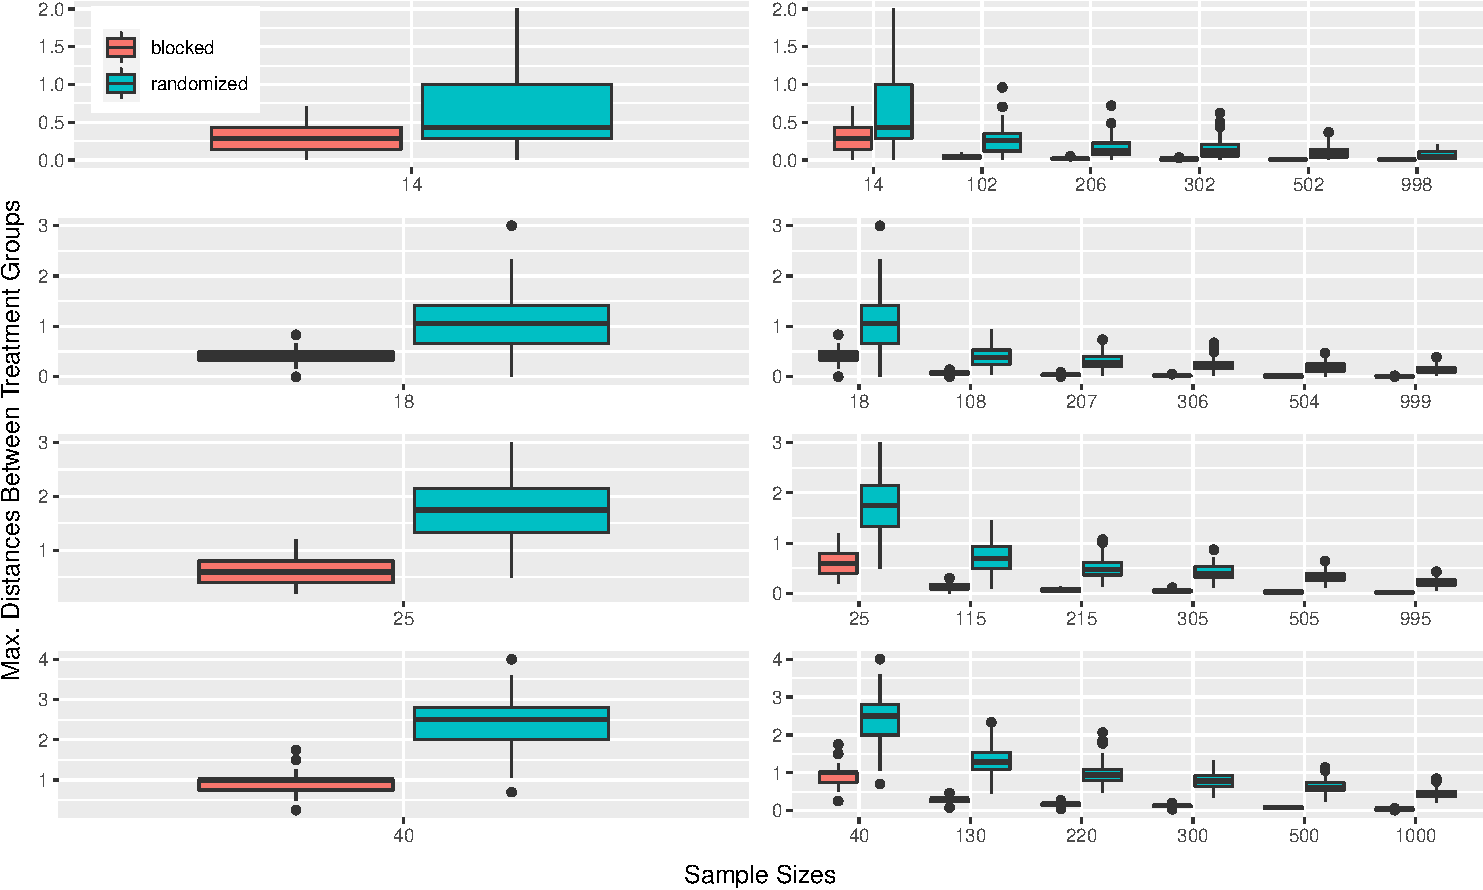
\includegraphics{dissertation_files/figure-latex/Boxplot-Law-Large-Numbers-1.pdf}
\caption{\label{fig:Boxplot-Law-Large-Numbers}Distances Between Treatment Group Means in Randomized and Blocked Data. Increasing Sample Size for 2 (Top Row), 3 (Second Row), 5 (Third Row), and 10 Treatment Groups (Bottom Row). Leftmost Pair on the Right Panel Is the Same as the Pair on the Left Panel\label{BoxLawLarNum}}
\end{figure}
For \(n = 998\) and 2 treatment groups, the largest distance between randomized treatment groups is 0.208, while the largest distance between blocked treatment groups is 0.01. For small samples and a large number of treatment groups, the difference between the two methods increases. For \(n = 40\) and 10 treatment groups, the largest distance between randomized treatment groups is 4, while the largest distance between blocked treatment groups is 1.75.

Figure \ref{HistLawLarNum} shows the count distributions of these imbalances. For 2 treatment groups (top left plot), almost all blocked treatment groups have a maximum distance of zero. Most randomized groups also have a maximum distance of zero, but it is a narrow majority. Almost 50 percent of randomized groups have distances greater than zero, though still lower than one. As the number of treatment groups increases, so do the distances between the treatment groups. Nonetheless, the vast majority of blocked groups still show a maximum distance of zero. Even for 10 treatment groups, more than 60 percent of the blocked groups are not distant from each other at all. This does not hold true for the randomized groups. For 3 treatment groups, the majority of distances are now above zero. For 5 groups, the majority of distances exceed 0.25. For 10 treatment groups, more than 60 percent of groups show a distance larger than 0.5.
\begin{figure}
\centering
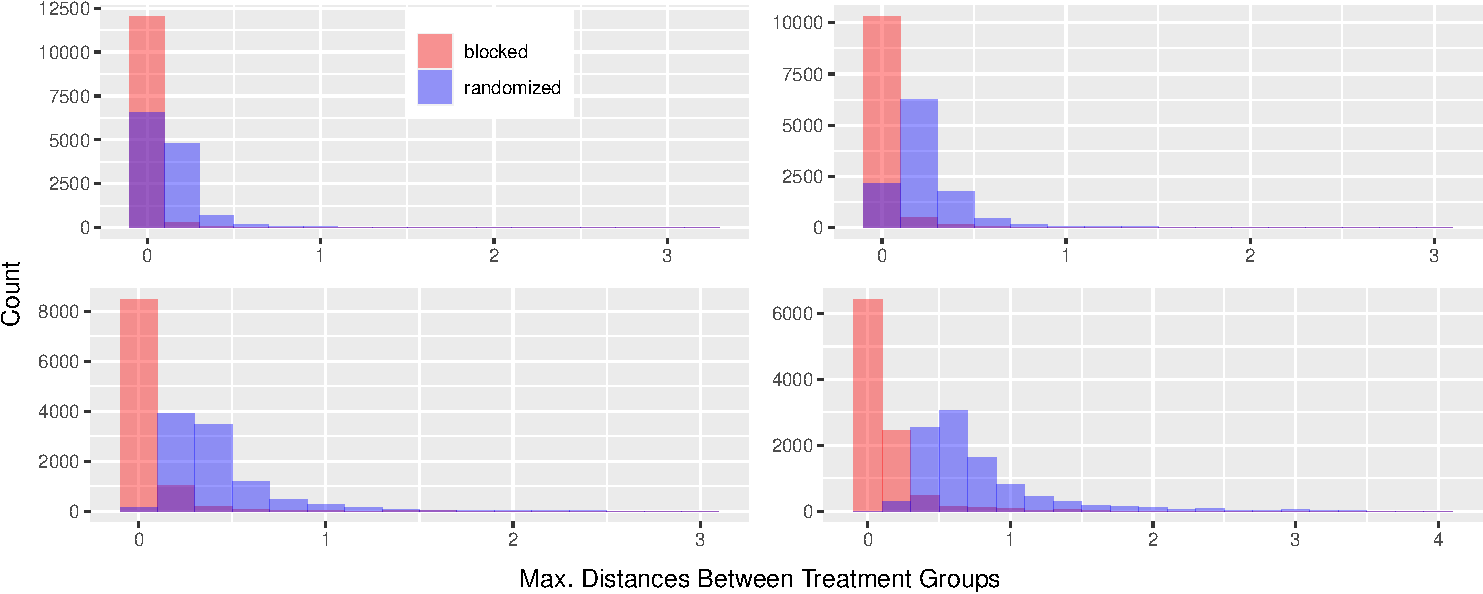
\includegraphics{dissertation_files/figure-latex/Hist-Law-Large-Numbers-1.pdf}
\caption{\label{fig:Hist-Law-Large-Numbers}Distribution of Treatment Group Differences in Randomized and Blocked Data for 2 (Top Left), 3 (Top Right), 5 (Bottom Left), and 10 Treatment Groups (Bottom Right). Overlapping Area Shown in Dark Purple.\label{HistLawLarNum}}
\end{figure}
\hypertarget{ordblock-theory-blocking-onthego}{%
\subsubsection{Blocking on the Go}\label{ordblock-theory-blocking-onthego}}

Survey experiments can utilize blocking in two ways: with all data present and `on the go'. The above data represents a simplified example of the former. All respondent covariate data have been collected before respondents are blocked into treatment groups, i.e.~covariate data are known for all respondents before assignment to treatment. Blocking `on the go' involves blocking respondents as they arrive for treatment at differing times. This is the case, for instance, for online survey experiments, where participants complete the survey at differing times, i.e.~they `trickle in' for treatment assignment as the experiment progresses. `Traditional' blocking can not be used here, since it relies on covariate information about the entire sample, which is not available. Instead, we need to block sequentially, or `on the go', as the experiment progresses. I use this method in the online survey experiment in chapter \ref{framing}.

Sequential blocking in political science is based on covariate-adaptive randomization, which varies probabilities based on knowledge about previous participants and the current participant (Chow \& Chang, 2007). Traditional covariate-adaptive approaches, such as the biased coin design (Efron, 1971) and minimization (Pocock \& Simon, 1975), assign the incoming participant to the treatment group with the fewest participants with identical covariate information. For discrete covariates, for instance, this takes the form of assigning all participants except the first one, \(q\), for covariate \(c\) with value \(d\) to a treatment group \(g\) with probability
\begin{align}
\text{prob}\left(g* = g\right) = \left(1 - \frac{q_{cdg}}{\sum^G_{g = 1} q_{cdg}}\right) \left(\sum_{g = 1}^G\left(1 - \frac{q_{cdg}}{\sum^G_{g = 1} q_{cdg}}\right)\right)^{-1}.
\end{align}
This works for discrete covariates as the number of possible covariate levels is finite. For continuous covariates, the number of possible covariate levels rises exponentially, which results in rare identical participants as they are unlikely to look the same. Blocking on continuous covariates is not possible with these traditional approaches (Eisele, 1995; Markaryan \& Rosenberger, 2010; Rosenberger \& Lachin, 2002). Moore \& Moore (2013) develop a method to do so by exploiting relationships between the current participant's covariate profile and those of all previously assigned participants. They define the similarity between participants with the MD between participants.

To aggregate pairwise similarity, they implement the mean, median, and trimmed mean of the pairwise MDs between the current participant and the participants in each treatment condition: Participants are indexed with treatment condition \(t\) using \(r \in \{1,...,R\}\). For each condition \(t\), they estimate an average MD between the current participant, \(q\), and the participants previously assigned. If the distance in terms of MD for the incoming participant is 2 in the control and 5 in the treatment condition, the incoming participant looks more similar to the control condition. To set the probability of assignment, Moore \& Moore (2013) calculate the mean MDs for each incoming participant, \(q\), for all treatment conditions, \(t\), and sort the treatment conditions by these averages. Randomization is biased towards conditions with high scores. For each value of \(k\) with \(k \in \{2,3,...,6\}\), the condition with the highest average MD is then assigned a probability \(k\) times larger than all other assignment probabilities.

Blocking is thus possible when all covariate information is known at the time of assignment and when it `trickles in' over time. Covariate information, however, is only one side of the coin. Researchers also need to take into consideration the characteristics of the variable to block on. Not all types of variables can and should be used the same way for blocking. Specifically, the current use of ordinal variables as blocking variables is somewhat problematic.

\hypertarget{ordblock-theory-ordinal}{%
\subsection{Ordinal Variables}\label{ordblock-theory-ordinal}}

Ordinal variables matter in surveys. One of the most important ordinal variables in political science surveys is education. It is widely established that education represents one of the major driving forces behind public opinion and political behavior, such as turnout or donations, in the U.S. (Abramowitz, 2010; Dawood, 2015; Druckman, Peterson, \& Slothuus, 2013; Fiorina \& Abrams, 2009; Fiorina, Abrams, \& Pope, 2011; King, 1997; Leighley \& Nagler, 2014). Ordinal variables are part of the larger framework of categorical variables. Categorical variables represent types of data which are commonly divided into three groups: nominal, interval, and ordinal variables. Nominal variables are categorical variables with two or more categories that are not intrinsically ordered. Examples include gender (Female, Male, Transgender etc.), race (African-American, White, Hispanic etc.), and party ID (Democrat, Republican, Independent) where the categories cannot be ordered sensibly into highest or lowest. Interval variables are ordered categorical variables with evenly spaced values. Examples include income (\$20,000, \$40,000, \$60,000, \$80,000 etc.), where the distance between \$20,000 and \$40,000 is the same as the distance between \$60,000 and \$80,000. Ordinal variables are ordered categorical variables where the spacing between values is not the same. Examples include education (Elementary School, Some High School, High School Graduate etc.) where the distance between ``Elementary School'' and ``Some High School'' is likely different than the distance between ``Some High School'' and ``High School Graduate''. Each subsequent category has quantitatively more education than the previous one, but the exact measure of the distances between the categories is unclear.

For statistical analysis, the categories of nominal variables are often turned into binary variables. This manipulation does not impose any unnatural ordering onto the variable and thus does not require any theoretical assumptions. Interval variables are often made numerical, which is statistically sound. It makes sense to assign numerical values such as 1, 2, 3, and 4 to income categories of \$20,000, \$40,000, \$60,000, and \$80,000 as the distance between each of these categories is identical for any adjacent pair. This translates perfectly into the numerical values with identical distances, i.e.~the distance between \$20,000 and \$40,000 is the same as the distance between 1 and 2. Ordinal variables are often treated as nominal variables by creating a new binary variable for one education category, for instance ``High School Graduate''. This approach ignores the ordered nature contained in ordinal variables and we would wrongly assume that the ordering of education categories is arbitrary. Ordinal variables are also often made numerical for analytic purposes. This is problematic because of their unevenly spaced categories. If the education categories ``Elementary School'', ``Some High School'', and ``High School Graduate'' were turned into the numerical values 1, 2, and 3, we would wrongly assume that the distances between the education categories correspond to these evenly spaced values. Do the numbers 1 to 3 really represent the distances between these categories? Perhaps the true spacing between some of the categories is so narrow they should not even be separate categories at all. We cannot answer this by making an arbitrary assumption that is not justified by the data. Alternatively, if ``Elementary School'', ``Some High School'', and ``High School Graduate'' were turned into three separate dummy variables, we would wrongly assume that there is no ordering to these values. In both cases, important information would be lost, which could lead to distortion (O'Brien, 1981). Unfortunately, these two approaches are commonly applied to ordinal variables in the social sciences. Liddell \& Kruschke (2018) for instance report that all articles published in 2016 in the Journal of Personality and Social Psychology (JPSP), Psychological Science (PS), and the Journal of Experimental Psychology that mention the term `Likert' analyze ordinal data with a metric or binary model. Doing so can cause inversions of effects as well as Type I and Type II errors (Lalla, 2017; Torra, Domingo-Ferrer, Mateo-Sanz, \& Ng, 2006). To truly use the ordinal nature of a variable, we need to use both its quantitative and its inherent unevenly spaced ordered aspects to make a more underlying description of the data possible (Agresti, 2010). To fill this gap, I propose an ordered probit model that estimates the latent continuous structure underlying ordinal variables.

\hypertarget{ordblock-theory-op}{%
\subsection{Ordered Probit Approach}\label{ordblock-theory-op}}

Many approaches in the literature on the analysis of ordinal variables incorporate the distribution of the variable categories (Agresti, 1996). The most promising suggestions focus on natural extensions of probit and logit models (Winship \& Mare, 1984) by assigning scores to be estimated from the data (Agresti, 1990) and quantifying each non-quantitative variable according to the empirical distributions of the variable, assuming the presence of a continuous underlying variable for each ordinal indicator (Lucadamoa \& Amenta, 2014). In fact, Agresti (2010) states ``that the type of ordinal method used is not that crucial'' but that the ``results may be quite different, however, from those obtained using methods that treat all the variables as nominal'' (p.~3). The same applies to methods which treat ordinal variables as interval (Gertheiss \& Tutz, 2008). This suggests that a probit or logit model is suitable to uncover the latent continuous variable underlying an ordinal variable, thereby using the ordinal information provided and respecting uneven distances. In the literature, this approach is focused exclusively on the analysis of ordinal variables as a response variable. I propose an ordered probit model that applies to ordinal variables as predictors. The workflow of the model is shown in Figure \ref{op-workflow}.

\vspace{0.2cm}

\ssp
\begin{figure}
\centering
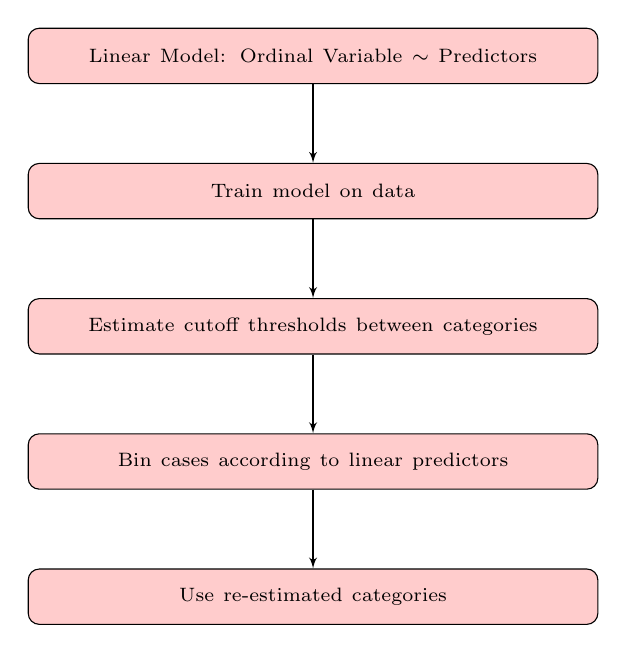
\begin{tikzpicture}
    \node [block2rw] (model) {\scriptsize{Linear Model: Ordinal Variable $\sim$ Predictors}};
    \node [block2rw, below =1cm of model] (train) {\scriptsize{Train model on data}};
    \node [block2rw, below =1cm of train] (cutoff) {\scriptsize{Estimate cutoff thresholds between categories}};
    \node [block2rw, below =1cm of cutoff] (bin) {\scriptsize{Bin cases according to linear predictors}};
    \node [block2rw, below =1cm of bin] (cats) {\scriptsize{Use re-estimated categories}};
    \coordinate[below=0cm of model] (modelc);
    \coordinate[above=0cm of train] (trainac);
    \coordinate[below=0cm of train] (trainbc);
    \coordinate[above=0cm of cutoff] (cutoffac);
    \coordinate[below=0cm of cutoff] (cutoffbc);
    \coordinate[above=0cm of bin] (binac);
    \coordinate[below=0cm of bin] (binbc);
    \coordinate[above=0cm of cats] (catsc);
    \path [line] (modelc) -- (trainac);
    \path [line] (trainbc) -- (cutoffac);
    \path [line] (cutoffbc) -- (binac);
    \path [line] (binbc) -- (catsc);
\end{tikzpicture}
\caption{Ordered Probit Workflow} 
\label{op-workflow}
\end{figure}
\dsp

\vspace{-0.4cm}

We need to estimate a linear combination of meaningful covariates as predictors and an ordinal variable as the dependent variable. We then train this model on externally and internally valid data to estimate cutoff thresholds between the ordinal categories and bin data cases according to the linear predictors. The binned cases determine which variable categories make sense, given the underlying latent continuous variable. We then replace the original categories with these re-estimated categories and conduct the statistical analysis of interest.

Notationally, let there be \(\bm{X}\), an \(n \times k\) matrix of explanatory variables. Let further \(\bm{Y}\) be observed on the ordered categories \(\bm{Y}_i \in [1,\ldots,k]\), for \(i=1,\ldots n\), and let \(\bm{Y}\) be assumed to be produced by the unobserved latent continuous variable \(\bm{Y^{cont}}\). \(\bm{Y^{cont}}\) is continuous on \(\mathfrak{R}\) from \(-\infty\) to \(\infty\). The `response mechanism' for the \(r^{th}\) category is \(Y=r \Longleftrightarrow \xi_{r-1} < Y^{cont} < \xi_r\). This requires there to be thresholds on \(R\):
\(Y^{cont}_i: \; \xi_0 \underset{a=1}{\longleftarrow\!\longrightarrow} \xi_1 \underset{a=2}{\longleftarrow\!\longrightarrow} \xi_2 \underset{a=3}{\longleftarrow\!\longrightarrow} \xi_3\ldots \xi_{A-1} \underset{a=A}{\longleftarrow\!\longrightarrow} \xi_A\). The vector of (unseen) utilities across individuals in the sample, \(\bm{Y^{cont}}\), is determined by a linear model of explanatory variables, \(Y^{cont} = X \beta + \mu\), where \(\bm{\beta} =[\beta_1,\beta_2,\ldots,\beta_p]\) does not depend on the \(\xi_j\) and \(\mu \sim F_{\mu}\). For the observed vector \(\bm{Y}\),
\begin{align}
p(Y \leq r|X) &= p(Y^{cont} \leq \xi_r) = p(X \beta + \mu \leq \xi_r) \nonumber\\
&= p(\mu \leq \xi_r+ X \beta) = F_{\mu}(\xi_r + X \beta)
\end{align}
is called the cumulative model because \(p(Y \leq \xi_r|X) = p(Y=1|X) + p(Y=2|X) + \ldots + p(Y=r|X)\). A logistic distributional assumption on the errors produces the ordered logit specification
\begin{align}
F_{\mu}(\xi_r - X' \beta) = P(Y \leq r|X) = [1+\exp(-\xi_r-X' \beta)]^{-1}. 
\end{align}
The likelihood function is
\begin{align}
L(\beta, \xi|X,Y) = \prod_{i=1}^{n}\prod_{j=1}^{A-1}\left[\Lambda(\xi_j + X_i' \beta) - \Lambda(\xi_{j-1} + X_i' \beta) \right]^{z_{ij}}
\end{align}
with \(\bm{\Lambda}\) denoting the logistic distribution and where \(z_{ij}=1\) if the \(i^\text{th}\) case is in the \(j^\text{th}\) category and \(z_{ij}=0\) otherwise. The thresholds on \(\mathfrak{R}\) partition the variable into regions corresponding to the ordinal categories. The linear model, \(\bm{Y^{cont}}\), bins the observations between these thresholds according to the linear predictors. In \texttt{R}, the ordered probit model can be implemented with the \texttt{polr} function from the \texttt{MASS} package (Ripley et al., 2020).

\hypertarget{ordblock-data}{%
\section{Data}\label{ordblock-data}}

I use the American National Election Studies (ANES) to implement the proposed ordered probit method. The ANES are the oldest continuous collection of national surveys on electoral behavior and attitudes in the US and are conducted before and after every US presidential and Congressional election by the University of Michigan and Stanford University. Data have been collected since 1948 in the attempt to understand voter behavior and candidate choice, among many others. The list of questions has been continually expanded and refined over the years. All ANES data are publicly available and the ANES are frequently used for high-profile publications (see for instance Jackman \& Spahn, 2018; Leighley \& Nagler, 2014). I apply the proposed ordered probit method to the 2016 ANES data and train a specified regression model on these data. This estimates the thresholds between each existing ANES education category and bins all observations according to the linear predictors to determine the education categories that make sense, based on the underlying latent continuous variable. This results in two sets of education categories: ANES and ordered probit (OP). The data are then blocked into three treatment groups to simulate a survey experiment environment. This process is conducted twice: once with the ANES categories, and once with the OP categories. To simulate sequential blocking, the order of observations is assumed to represent the sequential order of arrival for treatment. The estimation of group means and variances together with statistical tests reveals the suitability of this approach. Finally, I block the ANES data once more into two treatment groups and conduct a placebo regression to test model fitness further.

\hypertarget{ordblock-results}{%
\section{Results}\label{ordblock-results}}

Recall that we need to estimate a linear combination of meaningful covariates as predictors and an ordinal variable as the dependent variable. This model needs to be trained on externally and internally valid data. The ANES data have been shown to fulfill these criteria (Krupnikov \& Levine, 2014; Malhotra \& Krosnick, 2007). I train the following model on these data, using standard demographics in political science as predictors for all observations \(i\) with \(i = [1,\ldots,n]\):
\begin{align}
\text{Education}_i \sim & \,\beta_0 + \beta_1 \text{Gender}_i + \beta_2 \text{Race}_i + \beta_3 \text{Age}_i + \beta_4 \text{Income}_i \,+ \nonumber \\
& \beta_5 \text{Occupation}_i + \beta_6 \text{Party ID}_i + \epsilon_i
\end{align}
This estimates cutoff thresholds between the categories and bins data cases according to the linear predictors. The cutoff coefficients between each of the education categories are shown in Table \ref{education-categories}.
\begin{table}[!htbp] \centering 
  \caption{Ordered Probit Threshold Estimates} 
  \label{education-categories} 
\begin{tabular}{r@{}lr@{}lr@{}lr@{}l} 
\\[-1.8ex]\hline 
\hline \\[-1.8ex] 
\multicolumn{2}{c}{Thresholds} & \multicolumn{2}{c}{Coefficients} & \multicolumn{2}{c}{Standard Errors} & \multicolumn{2}{c}{t-values} \\ 
\hline \\[-1.8ex] 
Up to 1st $\mid$ & \,1st-4th & -7.&869 & 1.&024 & -7.&681 \\ 
1st-4th $\mid$ & \,5th-6th & -7.&146 & 0.&717 & -9.&965 \\ 
5th-6th $\mid$ & \,7th-8th & -5.&379 & 0.&326 & -16.&515 \\ 
7th-8th $\mid$ & \,9th & -4.&671 & 0.&253 & -18.&472 \\ 
9th $\mid$ & \,10th & -3.&920 & 0.&206 & -19.&070 \\ 
10th $\mid$ & \,11th & -3.&468 & 0.&188 & -18.&489 \\ 
11th $\mid$ & \,12th & -2.&984 & 0.&174 & -17.&100 \\ 
12th $\mid$ & \,HS grad & -2.&511 & 0.&166 & -15.&116 \\ 
HS grad $\mid$ & \,Some college & -0.&711 & 0.&154 & -4.&607 \\ 
Some college $\mid$ & \,Associate & 0.&384 & 0.&154 & 2.&500 \\ 
Associate $\mid$ & \,Bachelor's & 1.&045 & 0.&154 & 6.&766 \\ 
Bachelor's $\mid$ & \,Master's & 2.&478 & 0.&160 & 15.&538 \\ 
Master's $\mid$ & \,Professional & 4.&099 & 0.&177 & 23.&144 \\ 
Professional $\mid$ & \,Doctorate & 4.&838 & 0.&197 & 24.&589 \\ 
\hline \\[-1.8ex] 
\end{tabular} 
\end{table}
The ordered probit model uses the ordinal information with unevenly spaced distances provided and bins observations according to the estimated threshold coefficients, which in turn determines what education categories make sense given the underlying latent continuous variable. Figure \ref{DensEducLP} shows the distribution of this variable. As we can see, no cases fall lower than ``12th\textbar HS grad'' or higher than ``Master's\textbar Professional'', which results in a new set of model-estimated OP education categories that fit the data. We thus have two sets of education categories: the original ANES categories, and the model-estimated OP categories.
\begin{figure}
\centering
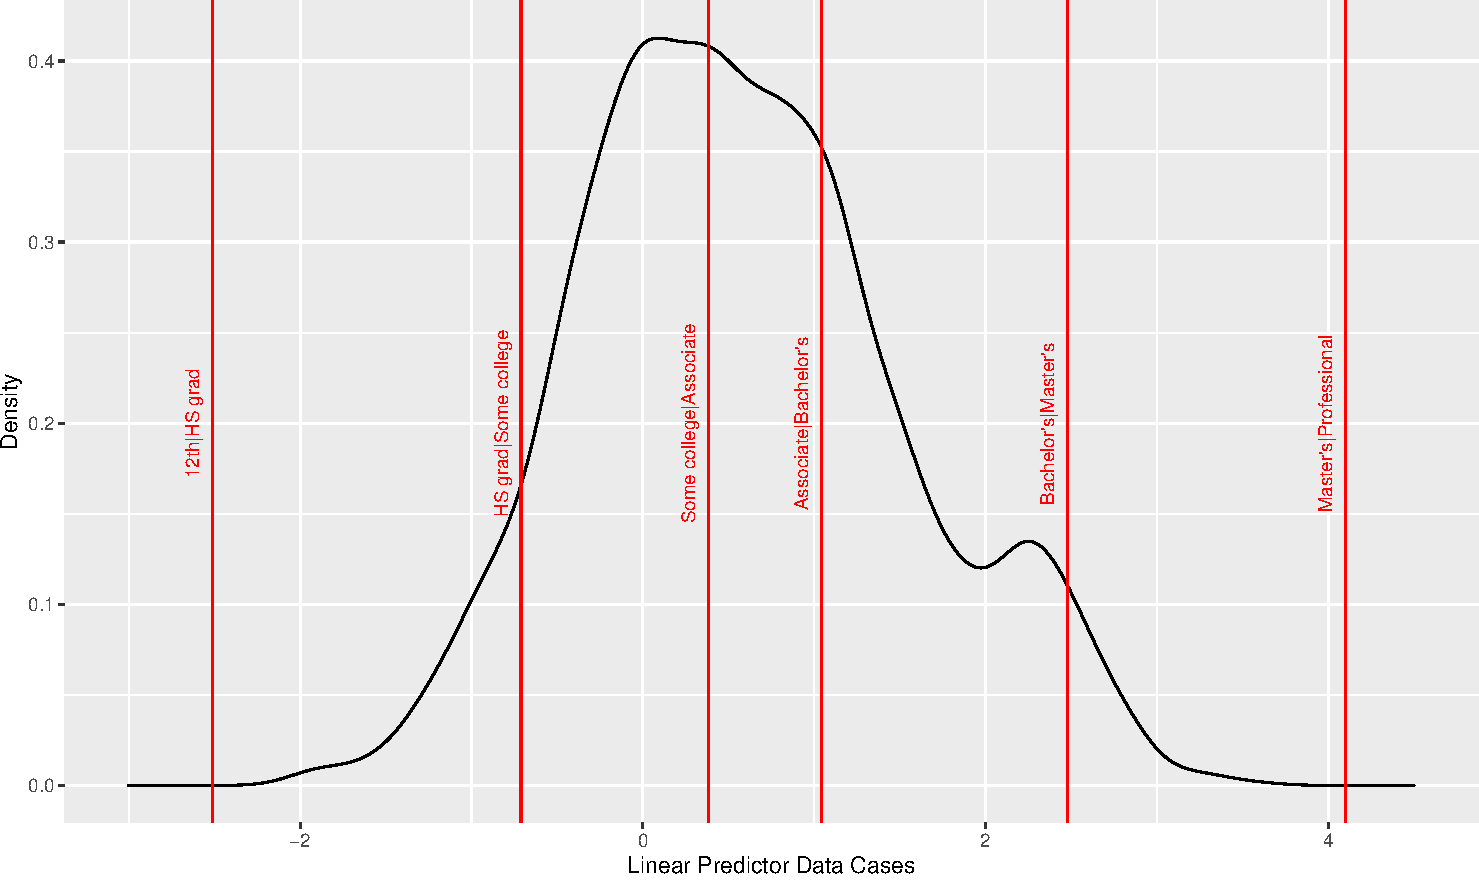
\includegraphics{dissertation_files/figure-latex/Density-Education-Categories-Linear-Predictors-1.pdf}
\caption{\label{fig:Density-Education-Categories-Linear-Predictors}Distribution of Education Linear Predictor Data Cases. Vertical Lines Indicate Threshold Coefficients. No Cases Fall Lower than `12th\textbar HS grad' or Higher than `Master's\textbar Professional'.\label{DensEducLP}}
\end{figure}
\begin{figure}
\centering
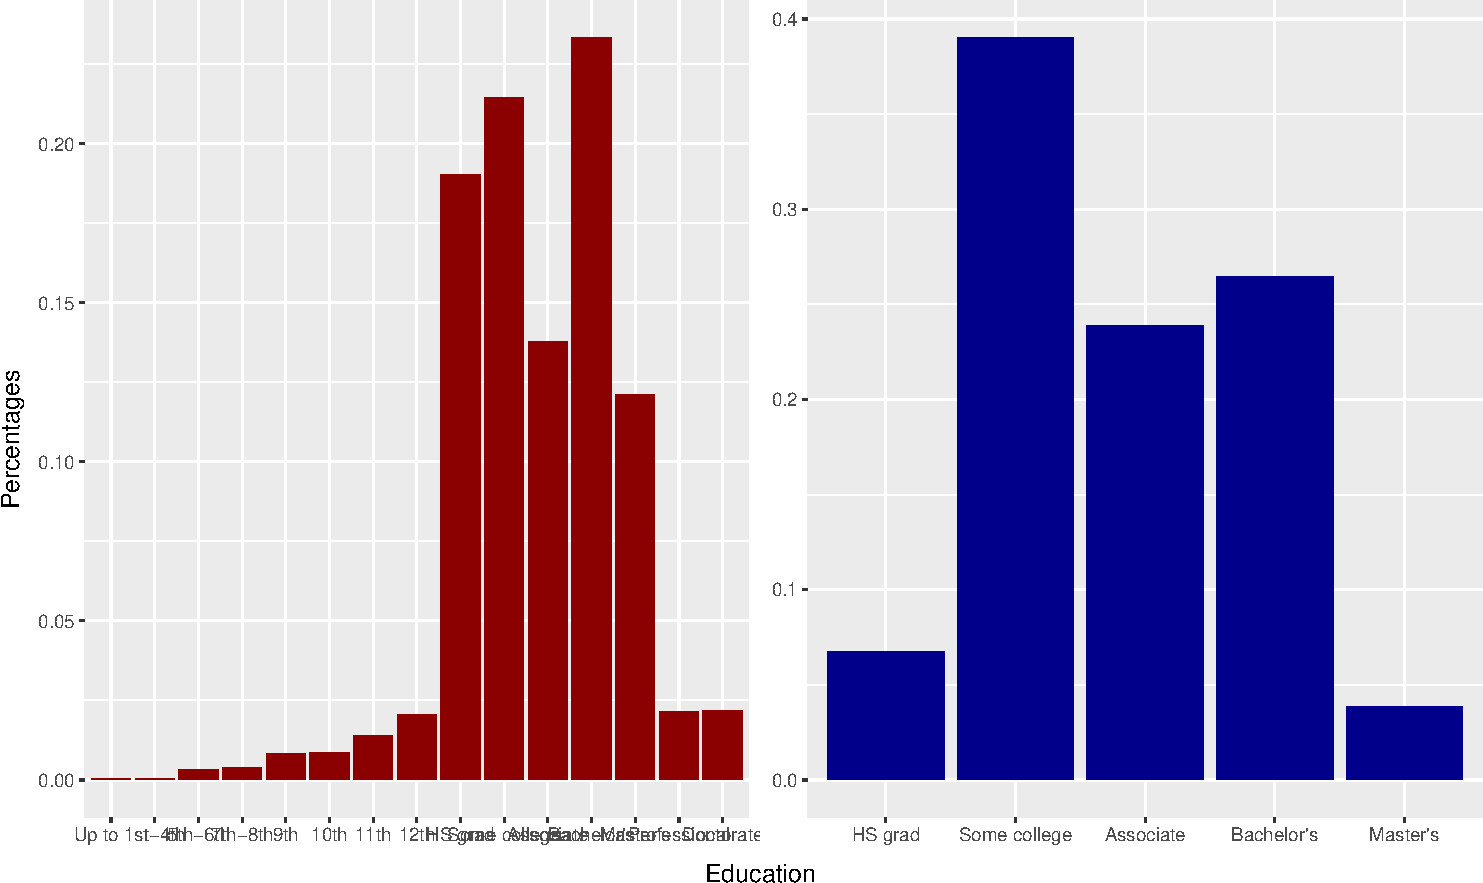
\includegraphics{dissertation_files/figure-latex/Barplot-Education-Categories-1.pdf}
\caption{\label{fig:Barplot-Education-Categories}Distribution of Education Categories. Original ANES Categories on the Left, Ordered Probit Estimated Categories on the Right. Categories Below `High School Graduate' and Above `Master's' Are Gone. OP Categories Can Now Be Used For Blocking.\label{BarEducCat}}
\end{figure}
Figure \ref{BarEducCat} shows the distributions of both sets. All categories `below' ``High School Graduate'' and `above' ``Master's'' are gone in the OP set because they do not fit the data. We can now use these estimated education categories as the basis for blocking. Assigning numerical values to the new categories is now justifiable because they are based on data-driven estimations. This allows us to block on numerical values with the MD, which would not be permitted on theoretical grounds without empirical justification. The following sections demonstrate how the newly estimated categories affect blocking and regression results.

\hypertarget{ordblock-data-blockdiff}{%
\subsection{Blocking Differences}\label{ordblock-data-blockdiff}}

We block the ANES on education into three treatment groups, once based on the original ANES education categories, and once based on the newly estimated OP education categories. We overall do not observe large differences between the ANES and OP variable proportions/means in each treatment group with the naked eye (see appendix Figures \ref{ANBlock1} to \ref{ANBlock3} for details).

To dig deeper, I run an Analysis of Variance (ANOVA) test on the numerical variables \texttt{Age} and \texttt{Feel\ Trump}. An ANOVA regression provides information about levels of variability within a regression model and forms a basis for tests of significance. As the name implies, ANOVA analyzes the variance in the data to look for differences by calculating the the sums of squares to measure the distances of each data point to the mean. The ratio of the sums of squares forms the F-statistic, which is used to gauge statistical significance.

I form a combined data set of all observations for each education set for each treatment group. This results in three data sets, i.e.~one per treatment group. The first data set contains all observations from the ANES set that were assigned to treatment group 1 and all observations from the OP set that were assigned to treatment group 1. The second data set contains all ANES and OP observations that were assigned to treatment group 2. The third data set contains all ANES and OP observations that were assigned to treatment group 3. Each data set contains the column \texttt{Education\ Set} which denotes the education set each observation belongs to. For each data set, I run an ANOVA regression of the numerical variables \texttt{Age} and \texttt{Feel\ Trump} on \texttt{Education\ Set} to test whether the choice of education set has a significant effect. Table \ref{aov-sum} shows a summary of the results. Almost none of the variable intercepts show statistical significance. An exception here is treatment group 2, which shows a \(p\)-value of 0.017 for \texttt{Feel\ Trump}. Overall, however, the differences between the treatment group means of the numerical variables \texttt{Age} and \texttt{Feel\ Trump} are not statistically significant for this sample size.
\begin{table}[!htbp] \centering  
 \caption{Summary of ANOVA Regression of Variable on ANES/OP Indicator. Differentiated by Treatment Group}   
 \label{aov-sum}
 \begin{tabular}{@{\extracolsep{5pt}} D{.}{.}{-3} D{.}{.}{-3} D{.}{.}{-3} D{.}{.}{-3} D{.}{.}{-3} D{.}{.}{-3} } 
 \\[-1.8ex]\hline 
 \hline \\[-1.8ex] 
 \multicolumn{1}{l}{} & \multicolumn{1}{l}{Df} & \multicolumn{1}{l}{Sum.Sq} & \multicolumn{1}{l}{Mean.Sq} & \multicolumn{1}{l}{F-value} & \multicolumn{1}{l}{p-value} \\ 
 \hline \\[-1.8ex] 
\multicolumn{1}{l}{\textbf{Age}} & & & & & \\ 
 \multicolumn{1}{l}{T1} & 1 & 0.107 & 0.107 & 0.000 & 0.985 \\
 \multicolumn{1}{l}{T1 Residuals} & 2,098 & 641,917.600 & 305.966 & & \\
 \multicolumn{1}{l}{T2} & 1 & 414.519 & 414.519 & 1.340 & 0.247 \\ 
 \multicolumn{1}{l}{T2 Residuals} & 2,098 & 648,946.600 & 309.317 & & \\
 \multicolumn{1}{l}{T3} & 1 & 427.954 & 427.954 & 1.401 & 0.237 \\
 \multicolumn{1}{l}{T3 Residuals} & 2,098 & 641,038.400 & 305.547 & & \\ 
 & & & & & \\
\multicolumn{1}{l}{\textbf{Feel Trump}} & & & & & \\  
 \multicolumn{1}{l}{T1} & 1 & 1,164.808 & 1,164.808 & 0.979 & 0.323 \\ 
 \multicolumn{1}{l}{T1 Residuals} & 2,098 & 2,496,492.000 & 1,189.939 & & \\
 \multicolumn{1}{l}{T2} & 1 & 7,054.667 & 7,054.667 & 5.699 & 0.017 \\ 
 \multicolumn{1}{l}{T2 Residuals} & 2,098 & 2,597,204.000 & 1,237.943 & & \\
 \multicolumn{1}{l}{T3} & 1 & 2,486.298 & 2,486.298 & 2.023 & 0.155 \\ 
 \multicolumn{1}{l}{T3 Residuals} & 2,098 & 2,577,984.000 & 1,228.782 & & \\ 
 \hline \\[-1.8ex]
 \end{tabular} 
 \end{table}
This leaves the non-numerical factor variables (e.g.~\texttt{Gender}, \texttt{Race} etc.). Since an ANOVA test is not possible for these variables, I conduct a binomial GLM regression here. The results are shown in Table \ref{glm-sum}. Contrary to the numerical variables, a large number of the \(p\)-values for the variable intercepts are highly significant. This includes all intercepts of \texttt{Race}, \texttt{Income}, \texttt{Occupation}, \texttt{Party\ ID}, \texttt{Min.\ Wage}, and \texttt{Country\ Track}. The only exceptions are \texttt{Gender} and \texttt{Pres.\ Approval}, where none of the intercepts in any treatment group (\texttt{Gender}) and only the intercepts in treatment groups 1 and 5 (\texttt{Pres.\ Approval}) reach statistical significance. The large number of statistically distinct categories indicates that a differentiation between education categories may be important for non-numerical factor variables.

\ssp

\footnotesize
\begin{longtable}{lr@{}lr@{}lr@{}lr@{}l}  
\caption{Summary of GLM Regression of Variable on ANES/OP Indicator. Differentiated by Treatment Group}    
\label{glm-sum}  
\\[-1.8ex]\hline  
\hline \\[-1.8ex]  
  & \multicolumn{2}{l}{Estimate} & \multicolumn{2}{l}{Std.Error} & \multicolumn{2}{l}{z-value} & \multicolumn{2}{l}{p-value} \\  
\hline \\[-1.8ex]  
\textbf{Gender} & & & & \\  
 T1 Intercept & 0.&091 & 0.&062 & 1.&481 & 0.&139 \\ 
 T1 & 0.&038 & 0.&087 & 0.&437 & 0.&662 \\ 
 T2 Intercept & 0.&126 & 0.&062 & 2.&035 & 0.&042 \\
 T2 & -0.&004 & 0.&087 & -0.&044 & 0.&965 \\
 T3 Intercept & 0.&134 & 0.&062 & 2.&159 & 0.&031 \\
 T3 & -0.&034 & 0.&087 & -0.&393 & 0.&694 \\ 
 & & & & \\  
\textbf{Race} & & & & \\  
 T1 Intercept & -1.&061 & 0.&071 & -15.&024 & 0.&000 \\
 T1 & -0.&035 & 0.&100 & -0.&351 & 0.&726 \\ 
 T2 Intercept & -1.&153 & 0.&072 & -15.&952 & 0.&000 \\
 T2 & 0.&041 & 0.&102 & 0.&407 & 0.&684 \\
 T3 Intercept & -1.&206 & 0.&073 & -16.&452 & 0.&000 \\
 T3 & -0.&005 & 0.&104 & -0.&052 & 0.&959 \\
   & & & & \\  
\textbf{Income} & & & & \\  
 T1 Intercept & 1.&334 & 0.&076 & 17.&557 & 0.&000 \\
 T1 & -0.&006 & 0.&107 & -0.&054 & 0.&957 \\
 T2 Intercept & 1.&227 & 0.&074 & 16.&649 & 0.&000 \\ 
 T2 & 0.&038 & 0.&105 & 0.&367 & 0.&714 \\ 
 T3 Intercept & 1.&398 & 0.&077 & 18.&058 & 0.&000 \\ 
 T3 & -0.&036 & 0.&109 & -0.&327 & 0.&744 \\
 & & & & \\  
\textbf{Employment} & & & & \\  
 T1 Intercept & -0.&421 & 0.&063 & -6.&678 & 0.&000 \\
 T1 & -0.&246 & 0.&091 & -2.&713 & 0.&007 \\
 T2 Intercept & -0.&567 & 0.&064 & -8.&831 & 0.&000 \\
 T2 & 0.&193 & 0.&090 & 2.&152 & 0.&031 \\
 T3 Intercept & -0.&588 & 0.&064 & -9.&126 & 0.&000 \\ 
 T3 & 0.&049 & 0.&091 & 0.&545 & 0.&586 \\ 
 & & & & \\  
  \textbf{Party ID} & & & & \\  
 T1 Intercept & 0.&530 & 0.&064 & 8.&297 & 0.&000 \\
 T1 & 0.&125 & 0.&091 & 1.&367 & 0.&172 \\
 T2 Intercept & 0.&655 & 0.&065 & 10.&065 & 0.&000 \\
 T2 & -0.&125 & 0.&091 & -1.&367 & 0.&172 \\
 T3 Intercept & 0.&609 & 0.&065 & 9.&421 & 0.&000 \\ 
 T3 & -0.&000 & 0.&091 & -0.&000 & 1.&000 \\ 
 & & & & \\  
\textbf{President} & & & & \\  
 T1 Intercept & -0.&210 & 0.&062 & -3.&388 & 0.&001 \\ 
 T1 & 0.&058 & 0.&088 & 0.&657 & 0.&511 \\ 
 T2 Intercept & -0.&008 & 0.&062 & -0.&123 & 0.&902 \\ 
 T2 & -0.&134 & 0.&087 & -1.&528 & 0.&126 \\ 
 T3 Intercept & -0.&103 & 0.&062 & -1.&666 & 0.&096 \\
 T3 & 0.&076 & 0.&087 & 0.&873 & 0.&383 \\ 
 & & & & \\  
\textbf{Minimum Wage} & & & & \\  
 T1 Intercept & -0.&613 & 0.&065 & -9.&480 & 0.&000 \\ 
 T1 & 0.&042 & 0.&091 & 0.&456 & 0.&649 \\ 
 T2 Intercept & -0.&465 & 0.&063 & -7.&340 & 0.&000 \\
 T2 & -0.&106 & 0.&090 & -1.&173 & 0.&241 \\
 T3 Intercept & -0.&685 & 0.&065 & -10.&472 & 0.&000 \\ 
 T3 & 0.&068 & 0.&092 & 0.&736 & 0.&462 \\
 & & & & \\  
\textbf{Country} & & & & \\  
 T1 Intercept & 0.&954 & 0.&069 & 13.&850 & 0.&000 \\ 
 T1 & -0.&005 & 0.&097 & -0.&049 & 0.&961 \\ 
 T2 Intercept & 1.&111 & 0.&071 & 15.&544 & 0.&000 \\ 
 T2 & -0.&055 & 0.&100 & -0.&552 & 0.&581 \\ 
 T3 Intercept & 0.&992 & 0.&069 & 14.&282 & 0.&000 \\
 T3 & 0.&059 & 0.&099 & 0.&593 & 0.&553 \\ 
 \hline \\[-1.8ex]
 \end{longtable}
\dsp

\normalsize

Overall, the evidence is mixed. While blocking on two different sets of education categories does not result in significantly differing means for the numerical variables, it does yield statistically significant differences between the factor variable proportions.

\hypertarget{ordblock-data-plac}{%
\subsection{Placebo Regression}\label{ordblock-data-plac}}

To further test the usefulness of the ordered probit categories, I conduct a placebo regression. Placebo tests are most commonly used for difference-in-differences estimators and are falsification tests to analyze whether an effect exists that should not exist (Bertrand, Duflo, \& Mullainathan, 2004; Mills \& Patterson, 2009; Rothstein, 2010). The placebo treatment should be unrelated to the model or method being studied (Hartman \& Hidalgo, 2018; Mora \& Reggio, 2019; Rosenbaum, 2002). In the effort to conduct an analysis that is separate from the previous section, I block the 2016 ANES data anew on education, this time into two treatment groups. As before, this is done separately for the original ANES and the OP education categories. We then model the following OLS regression on the feeling thermometer towards Donald Trump as the Republican presidential candidate for all observations \(i\) with \(i = [1,\ldots,n]\):
\begin{align}
\text{Feel Trump}_i \sim & \,\beta_0 + \beta_1 \text{Group}_i + \beta_2 \text{Democrat}_i + \beta_3 \text{Republican}_i + \beta_4 \text{Income}_i \,+ \nonumber \\ 
& \beta_5 \text{Male}_i + \beta_6 \text{White}_i + \beta_7 \text{Black}_i + \beta_8 \text{Hispanic}_i.
\end{align}
The \texttt{Group} variable indicates the two differing sets of education categories and is a placebo treatment, i.e.~I did not conduct an experiment and no actual treatment was administered. Instead, I created the \texttt{Group} variable, randomly `assigned' observations to the two treatment groups, and then used this variable as an explanatory variable. The treatment is thus completely artificial, which means the difference between both treatment groups should be zero, i.e.~there should be no significant differences between the \texttt{Group} regression coefficients for the two education sets. The null hypothesis thus assumes that there is no effect. To test this, each blocking/regression process for each set of categories is repeated 1,000 times. The distribution of the placebo treatment indicator (\texttt{Group}) is visualized in Figure \ref{DensPlacTreat}.
\begin{figure}
\centering
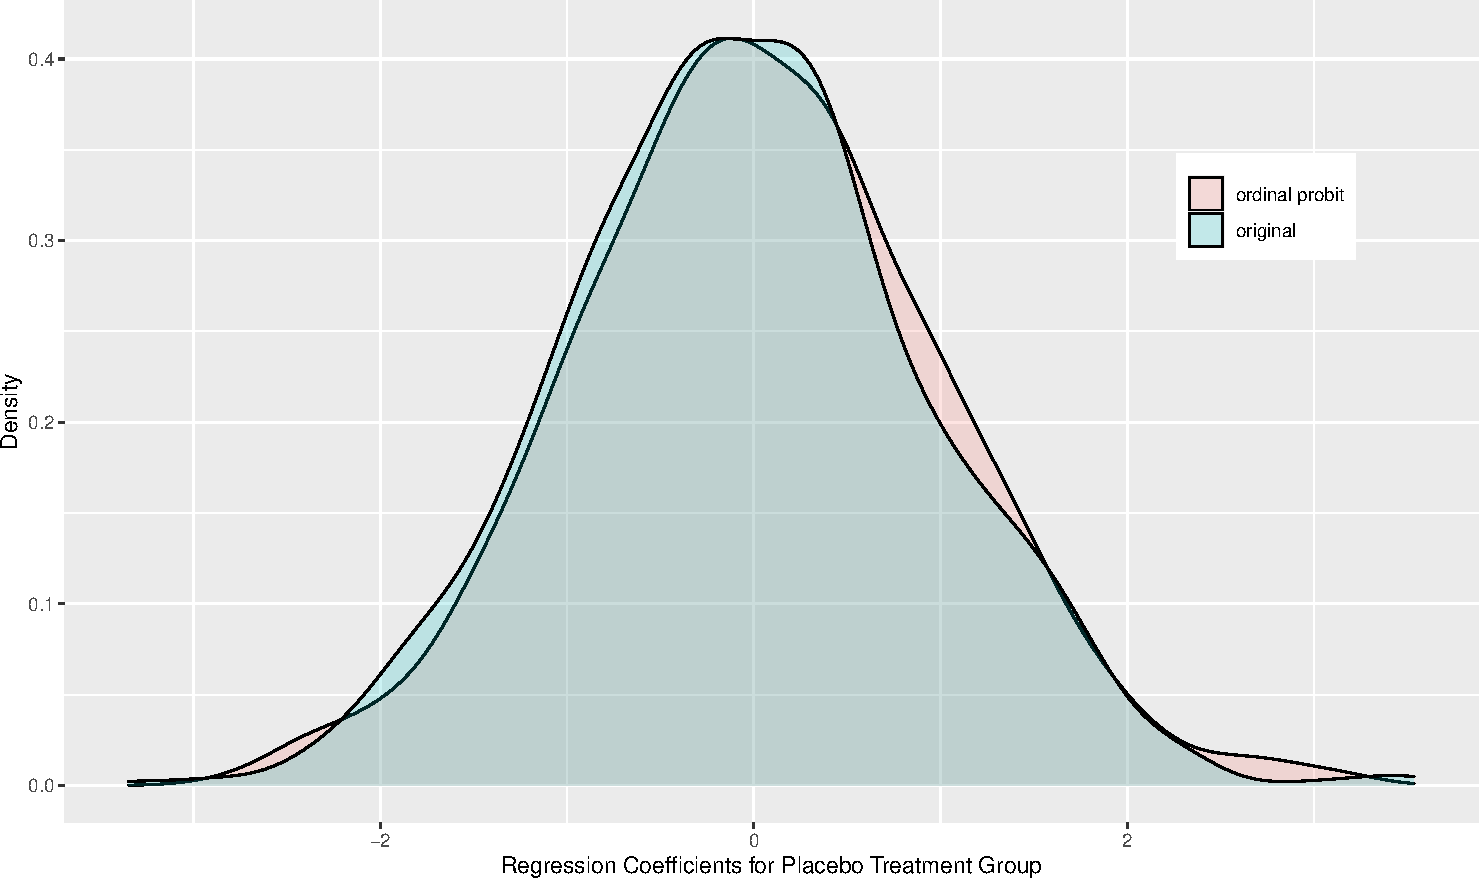
\includegraphics{dissertation_files/figure-latex/Density-Plot-Placebo-Treatment-1.pdf}
\caption{\label{fig:Density-Plot-Placebo-Treatment}Distribution of Placebo Treatment Coefficients by Education Set. Overlapping Area Shown in Dark Purple.\label{DensPlacTreat}}
\end{figure}
Both distributions center around zero, as is the statistical expectation. Upon closer inspection, however, the ordered probit categories are closer to the true value of zero than the ANES categories on both mean (0.019 v. -0.05) and median (-0.01 v. -0.07). This indicates slightly superior performance by the ordered probit categories, as they more closely approach the true value when used in a regression.

\hypertarget{ordblock-conclusion}{%
\section{Conclusion}\label{ordblock-conclusion}}

I set out to improve the use of ordinal variables to block respondents into treatment groups in survey experiments. Survey experiments depend on balance of covariates between treatment groups to allow the estimation of causal effects. Randomization ensures balance for large samples but becomes problematic for small samples. Blocking greatly alleviates this problem.

Blocking naturally depends on covariates. One of the most important covariates in political science is education. Out of convenience, education is often converted to a numerical variable for regressions in practice. Due to the special nature of education as an ordinal variable, such an approach is potentially problematic as ordinal variable categories are not evenly spaced. The distance between the education categories ``Elementary School'' and ``Some High School'' is very likely not the same as the distance between ``Some High School'' and ``High School Graduate''. Converting these three categories to the numerical values 1, 2, and 3, however, assumes evenly spaced distances. This could lead to a misrepresentation of the data.

As an alternative, I proposed an ordered probit approach whereby we estimate the latent underlying continuous variable underneath education. This estimates cutoff thresholds between the education categories, bins observations according to linear model predictors, and results in a new set of education categories that fit the data and represent the latent underlying continuous variable with its unevenly spaced distances. I applied this approach to the 2016 ANES data, resulting in two sets of education categories: the original ANES categories, and the newly estimated OP categories. I subsequently blocked both sets into three treatment groups and analyzed the group means and variances. While the numerical variables do not show statistically distinct intercepts, most of the factor variables do. This might indicate that the re-estimation of education categories is meaningful, but the evidence is unclear. I also ran a placebo regression 1,000 times to conduct a falsification test. This shows distributions of the placebo treatment variable around the statistically expected zero but also reveals the OP variable to be closer to zero than the ANES variable for both mean and median. This might indicate slightly superior performance by the OP method.

In all, the results are unclear. Some findings support the notion that the re-estimation of ordinal variable categories with an ordered probit approach matters, while others negate it. The next chapter will use the OP approach to address multiple imputation with ordinal variables.

\hypertarget{ordmiss}{%
\chapter{QUALITY COMPARISON OF MAJOR MISSING DATA SOLUTIONS WITH A PROPOSED NEW METHOD FOR ORDINAL VARIABLES}\label{ordmiss}}

\hypertarget{ordmiss-intro}{%
\section{Introduction}\label{ordmiss-intro}}

Missing data are ubiquitous in survey research (Allison, 2002; Raghunathan, 2016). Respondents frequently refuse to answer questions, select ``Don't Know'' as a response option, or drop out during the response collection process (Honaker \& King, 2010). Missingness in data sets poses a big problem since such data cannot be appropriately analyzed with statistical software without pre-processing (Little \& Rubin, 2002; Molenberghs \& Kenward, 2007). Scholars have developed several ways to treat missing data. These can be roughly categorized into deletion, single imputation, and multiple imputation.

Deletion, also called case-wise deletion, list-wise deletion or complete case analysis, simply removes all observations with missing values from the sample. Single imputation concerns the replacement of missing values with substitute estimates such as the mean, regression coefficients, or values from randomly drawn `similar' respondents in the data. Multiple imputation estimates missing values from conditional distributions and subsequently averages the results into a single parameter of inference (Fay, 1996; King, Honaker, Joseph, \& Scheve, 2001; Rubin, 1976).

Multiple imputation has become the state of the art in missing data management since it accounts for and incorporates uncertainty around the estimated imputations through repeated draws (Andridge \& Little, 2010; Graham \& Schafer, 1999; Schafer \& Graham, 2002; White et al., 2011). This is missing from single imputation techniques which treat the single estimated replacement value as a de-facto data entry on par with observed values. Uncertainty is not reflected in the imputed values, which leads to biased standard errors and confidence intervals (Gill \& Witko, 2013; Kroh, 2006). Similarly, list-wise deletion has been shown to induce bias with political data (Bodner, 2008; Collins, Schafer, \& Kam, 2001; Pigott, 2001; Rees \& Duke-Williams, 1997; Reilly, 1993).

However, parametric multiple imputation as applied by the most popular imputation packages in \texttt{R} is not necessarily always the most suitable method for all types of variables. For discrete data, multiple hot deck imputation, a combination of the single imputation method hot decking and multiple imputation, proves more precise as it avoids the common multiple imputation technique of imputing discrete data on a continuous scale (Gill \& Cranmer, 2012). The latter turns discrete variables into continuous variables which changes their nature and can result in non-observable and biased imputation values with artificially smaller standard errors (Fuller \& Kim, 2005; Kim, 2004; Kim \& Fuller, 2004). Multiple hot deck imputation on the other hand preserves the integrity of discrete data, does not change the size of standard errors, and produces more accurate imputations. It estimates affinity scores for each missing value to measure how similar a respondent with a missing value is to another respondent across all variables except the missing one.

However, multiple hot deck imputation does not account for ordinal variables as its affinity score algorithm assumes even distances between categories in discrete data. This assumption is not warranted for ordinal variables. I propose a method designed to impute discrete missing data specifically from ordinal variables. Because of the success of multiple hot deck imputation in its applicability to missing data with discrete variables with a small number of categories (Gill \& Cranmer, 2012), this method is based on multiple hot deck imputation and adapted to account for the specific circumstances of ordinal variables. Based on the ordered probit model approach described in section \ref{ordblock-theory-op}, it applies a scaled solution with newly estimated numerical thresholds from an assumed underlying latent continuous variable to measure the distances between the categories and calculate affinity scores.

\hypertarget{ordmiss-theory}{%
\section{Theory}\label{ordmiss-theory}}

\hypertarget{ordmiss-theory-mechanisms}{%
\subsection{Missing Data Mechanisms}\label{ordmiss-theory-mechanisms}}

Let there be \(\bm{X}\), an \(n \times v\) matrix with data on \(n\) respondents for \(v\) variables. Let there also be the response indicator \(\bm{R}\) as an \(n \times v\) matrix with values of 0 or 1. Let their respective elements be denoted by \(x_{ij}\) and \(r_{ij}\), with \(i = 1, ..., n\) and \(j = 1, ..., v\). If \(x_{ij}\) is observed, \(r_{ij} = 1\). If \(x_{ij}\) is missing, \(r_{ij} = 0\). All elements where \(r_{ij} = 0\) make up the missing data, \(\bm{X^{miss}}\). All elements where \(r_{ij} = 1\) make up the observed data, \(\bm{X^{obs}}\). Together, \(\bm{X^{obs}}\) and \(\bm{X^{miss}}\) form the complete data \(\bm{X}\). Missing data can then generally be described by \(\text{prob}(\bm{R} = 0 | \bm{X^{obs}}, \bm{X^{miss}}, \bm{\theta})\), i.e.~the probability of missing data depends on the observed data, the missing data, and a vector of unknown parameters. Depending on the mechanism by which data is missing, this expression can be further simplified. Data can be missing by three basic mechanisms: It can be missing completely at random (MCAR), missing at random (MAR), or missing not at random (MNAR). Researchers need to make assumptions about how the data came to be missing.

The general missing data expression can be simplified under the MCAR assumption to \(\text{prob}(\bm{R} = 0 | \bm{\theta})\), i.e.~the generic probability of missing data, independent of the data themselves and only dependent on \(\bm{\theta}\). A MCAR assumption in political science surveys is rare and requires justification as missing data most often occur systematically. Respondents are known to withhold sensitive data, for instance in the attempt to hide private information (income, sexual orientation) or out of fear of political or social repercussions in the community (union membership, support for polarizing political candidates) (Groves et al., 2009). Such information is often not refused randomly but occurs only in specific subsets of respondents. Answers criticizing the authorities, for instance, tend to be missing in surveys in non-democratic states, while the state-loyal responses are present.

It is more commonly assumed among researchers that data are MAR. MAR means missing data are related to the observed but not the unobserved data. In practical terms, this for instance means missing data on income can be related to observed data on education or occupation. Here, the missing data are not a random sample of the entire data. MAR transforms the general missing data expression to \(\text{prob}(\bm{R} = 0 | \bm{X^{obs}}, \bm{\theta})\), i.e.~the chances of missing data depend on the observed data and \(\bm{\theta}\).

Finally, data can be MNAR.\footnote{Data MNAR is also sometimes called `non-ignorable' (see for instance Gill \& Cranmer, 2012 and Allison, 2002).} This is the case when missing data are related to unknown and/or unobserved parameters. Continuing the example of missing data on income, under MNAR we do not observe data on education or occupation that can be used to fill the missing income data slot. In the case of data MNAR, the general missing data expression remains unchanged, \(\text{prob}(\bm{R} = 0 | \bm{X^{obs}}, \bm{X^{miss}}, \bm{\theta})\), i.e.~the missingness of data depends on the observed data, the missing data, and \(\bm{\theta}\).

As mentioned above, the assessment of the missing data mechanism underlying any respective data comes from researchers and their understanding of the data generating process. The statistical methods to address missing data can be broadly categorized into deletion, imputation, and multiple imputation.

\hypertarget{ordmiss-theory-delete}{%
\subsection{List-Wise Deletion}\label{ordmiss-theory-delete}}

One of the most common methods of handling missing data in quantitative political science is list-wise deletion. This involves the removal of any incomplete observations, thereby reducing the sample size. The resulting sample is then ready for analysis.

List-wise deletion is not biased with data MCAR as it removes a random sample of the population, but it reduces the degrees of freedom and might hinder sub-group analysis (Allison, 2002; King et al., 2001; Little \& Rubin, 2002; Schafer \& Graham, 2002). When data are MAR or MNAR, list-wise deletion is always biased, since the observed data is tilted towards respondents with characteristics that make them more likely to respond. Whether this bias is trivial or substantial depends on the research and circumstances in question (Collins et al., 2001; Diggle \& Kenward, 1994; Glynn, Laird, \& Rubin, 1993; Graham, Hofer, Donaldson, MacKinnon, \& Schafer, 1997; Robins, Rotznitzky, \& Scharfstein, 1998).

While the bias inserted by list-wise deletion in each individual data analysis may not necessarily be drastic, studies have shown that it can be so severe as to alter substantive conclusions (Brown, 1994; Graham, Hofer, \& MacKinnon, 1996; Honaker \& King, 2010; Wothke, 2000). Even if that were not or only rarely the case and most data were MCAR, reducing the sample size is generally never a recommended approach as, among other aspects, standard errors from regression models are inflated. As King et al. (2001) put it, the result of list-wise deletion ``is a loss of valuable information at best and severe selection bias at worst'' (p.~49). In \texttt{R}, list-wise deletion can be implemented with the base function \texttt{na.omit}.

\hypertarget{ordmiss-theory-singimpute}{%
\subsection{Single Imputation}\label{ordmiss-theory-singimpute}}

Single imputation means replacing missing data with substituted values, i.e.~the structural opposite of deletion. Imputation requires a predictive distribution, based on the observed data, from which value substitutions are picked. Single imputation, regardless of its exact nature, is not recommended to impute missing data since, similar to deletion, it downward biases standard errors and confidence intervals (Honaker \& King, 2010). Crucially, uncertainty is not reflected in the imputed values (Little \& Rubin, 2002). The following is a mere selection of the most common single imputation methods and makes no claim of completeness. Since single imputation is widely condemned as a general imputation method and as my focus lies on multiple imputation, they are also brief.

\hypertarget{ordmiss-theory-impute-mean}{%
\subsubsection{Mean}\label{ordmiss-theory-impute-mean}}

Mean imputation, sometimes also called unconditional mean imputation, involves replacing missing values within cells with the mean of the observed values, so \(\bm{X^{miss}} = \bm{\overline{X^{obs}}}\). While it does not change the mean of the sample, this method distorts the empirical distribution of \(\bm{X}\), which in turn produces biased estimates of any non-linear quantities such as variances and covariances (Haitovsky, 1968). It is also bound to be inaccurate in most cases, since few values generally fall exactly on the mean, and can be non-sensical for discrete variables (Efron, 1994). Mean imputation can be done in many ways in \texttt{R}, for instance with the \texttt{impute} function in the \texttt{Hmisc} package or by setting \texttt{method\ =\ "mean"} in the \texttt{mice} function in the \texttt{mice} package.

\hypertarget{ordmiss-theory-impute-regress}{%
\subsubsection{Regression}\label{ordmiss-theory-impute-regress}}

Imputation by regression, sometimes also called conditional mean imputation, imputes missing values conditional on observed values. Researchers predict observed variable values based on other variables, while the fitted values from the regression model are then used to impute variable values where they are missing. Let there be an explanatory variable \(x\) in a multiple regression model. Assume that \(x\) contains missing values, \(x^{miss}\), and observed values, \(x^{obs}\). We regress \(x^{obs}\) on the other explanatory variables and use the estimated equation to generate predicted values for \(x^{miss}\), \(x^{pred}\). \(x^{pred}\) then replace \(x^{miss}\), thus completing the data set. While more accurate than mean imputation, particularly for large samples with data MCAR, regression imputation nonetheless suffers from the same flaw that accompanies all single imputation approaches: Uncertainty is not reflected in the imputed values (Horton \& Kleinman, 2007).

Differing variations of imputation by regression exist in \texttt{R}, such as the \texttt{aregImpute} function in the \texttt{Hmisc} package, which performs additive regression, and setting \texttt{method\ =\ "norm.predict"} in the \texttt{mice} function to conduct linear regression. The \texttt{predict} function in base \texttt{R} also applies linear regression imputation.

\hypertarget{ordmiss-theory-impute-hd}{%
\subsubsection{Hot Decking}\label{ordmiss-theory-impute-hd}}

Hot deck imputation was developed in the 1970s and replaces missing values with values from similar respondents in the sample (Ernst, 1978; Ford, 1983). It is called `hot decking' as a reference to taking draws from a deck of matching computer punch-cards. The deck was `hot' since it was currently being processed, as opposed to pre-collected or `cold' data (Andridge \& Little, 2010; Little \& Rubin, 2002). In the most general version, researchers select all respondents that are `similar' to a respondent with missing data and randomly draw one of those respondents (with replacement) to fill in the missing value. The respondent with the initially missing value is termed the \textit{recipient}, while the `similar' respondent is called the \textit{donor}. Variations of the method include hot decking within adjustment cells, by nearest neighbor, and sequentially ordered by a covariate (Cox, 1980; David, Little, Samuhel, \& Triest, 1986; Kaiser, 1983; Kalton \& Kish, 1981; Rockwell, 1975).

Contrary to mean or regression imputation, hot deck imputation preserves the integrity of the data, i.e.~only actually observed values are used to fill in missing slots (Bailar \& Bailar, 1997). In both other single imputation methods, it is possible and sometimes even likely that missing values are replaced by values not found amongst the observed values. Contrary to regression imputation, hot decking also does not require a fitted model and is thus less vulnerable to model misspecification. However, hot decking does necessitate the existence of at least some donors for a respondent at every variable value that is missing. With a lot of missing data and few `similar' matches, the accuracy of hot decking greatly decreases (Young, Weckman, \& Holland, 2011). Hot decking works best for discrete data as continuous data are very unlikely to be matched or `similar', though the definition of what might constitute a `similar' respondent is somewhat subjective (Marker, Judkins, \& Winglee, 2002). As is the case with all single imputation methods, uncertainty is not reflected in the imputed values. Selecting the initial sample of `similar' respondents and the subsequent random sampling from that subsampling are treated as factual responses, which leads to smaller standard errors and confidence intervals than statistically valid (Little \& Rubin, 2002).

To my knowledge, there is currently no \texttt{R} package that applies single hot deck imputation. Nonetheless, variations of hot decking are still in use by some government statistics agencies such as the National Center for Education Statistics (for parts of the Current Population Survey) or the U.S. Bureau of the Census (NCES, 2002; USBC, 2002).

\hypertarget{ordmiss-theory-multimpute}{%
\subsection{Multiple Imputation}\label{ordmiss-theory-multimpute}}

Multiple imputation was invented by Rubin in the 1970s to account for the absence of uncertainty in single imputation methods and allow more accurate standard error estimates. It fills missing values with a predictive model that includes observed data and prior knowledge (Honaker \& King, 2010). Over the time of its development, it has become the dominant sophisticated strategy for handling missing data (Dempster, Laird, \& Rubin, 1977; Glynn et al., 1993; Heitjan \& Rubin, 1991; Little \& Rubin, 2002; Rubin, 1976, 1987, 1996; Rubin \& Schenker, 1986). Multiple imputation involves three general steps:

\vspace{0.3cm}
\begin{adjustwidth*}{+0.5cm}{+0.5cm}
\ssp
\begin{enumerate}
\item \noindent Impute data with missing values $m$ times. This results in $i$ complete
 \begin{sloppypar}\hspace{0.5cm} data sets (with $i = 1, ..., m$).\end{sloppypar}
\item Analyze each of the $i$ complete data sets.
\item Combine the results from each of the $i$ analyses into one collective result.
\end{enumerate}
\end{adjustwidth*}
\vspace{0.3cm}

\ssp
\begin{figure}
\centering
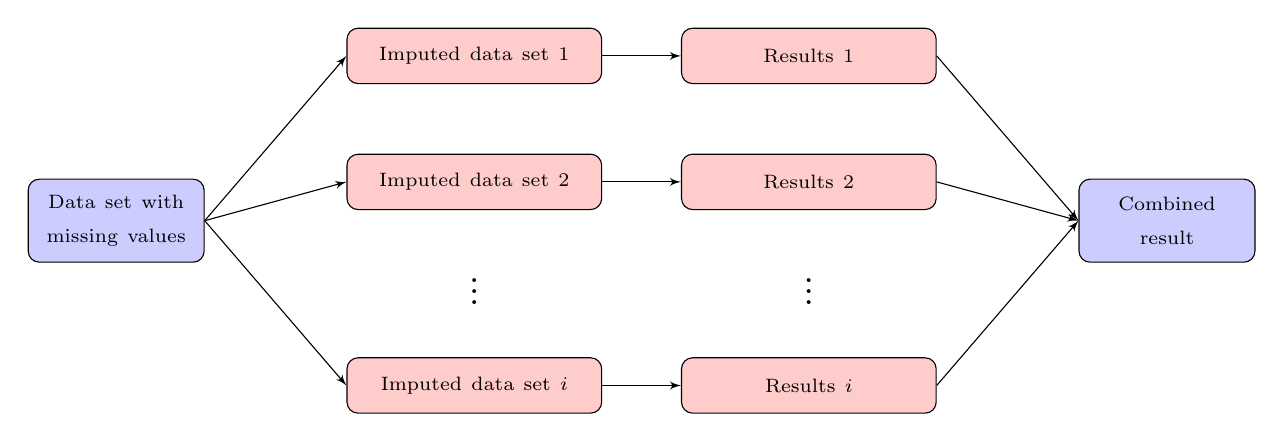
\begin{tikzpicture}
    \node [block3] (ds) {\scriptsize{Data set with missing values}};
    \node [block2r, above right=1.2cm and 1.8cm of ds] (imp1) {\scriptsize{Imputed data set 1}};
    \node [block2r, above right=-0.4cm and 1.8cm of ds] (imp2) {\scriptsize{Imputed data set 2}};
    \node [block2r, below right=1.2cm and 1.8cm of ds] (impi) {\scriptsize{Imputed data set $i$}};
    \coordinate[right=0cm of ds] (dsc);
    \coordinate[left=0cm of imp1] (imp1lc); 
    \coordinate[left=0cm of imp2] (imp2lc); 
    \coordinate[left=0cm of impi] (impilc); 
    \path [line] (dsc) -- (imp1lc);
    \path [line] (dsc) -- (imp2lc);
    \path (imp2) --node[auto=false]{\Large{\vdots}} (impi);
    \path [line] (dsc) -- (impilc);
    \node [block2r, right=1cm of imp1] (results1) {\scriptsize{Results 1}};
    \node [block2r, right=1cm of imp2] (results2) {\scriptsize{Results 2}};
    \node [block2r, right=1cm of impi] (resultsi) {\scriptsize{Results $i$}};
    \coordinate[right=0cm of imp1] (imp1rc);
    \coordinate[right=0cm of imp2] (imp2rc);
    \coordinate[right=0cm of impi] (impirc);
    \coordinate[left=0cm of results1] (results1lc); 
    \coordinate[left=0cm of results2] (results2lc); 
    \coordinate[left=0cm of resultsi] (resultsilc); 
    \path [line] (imp1rc) -- (results1lc);
    \path [line] (imp2rc) -- (results2lc);
    \path (results2) --node[auto=false]{\Large{\vdots}} (resultsi);
    \path [line] (impirc) -- (resultsilc);
    \node [block3, below right=1.2cm and 1.8cm of results1] (results) {\scriptsize{Combined result}};
    \coordinate[left=0cm of results] (resultsc);
    \coordinate[right=0cm of results1] (results1rc);    
    \coordinate[right=0cm of results2] (results2rc);    
    \coordinate[right=0cm of resultsi] (resultsirc);    
    \path [line] (results1rc) -- (resultsc);
    \path [line] (results2rc) -- (resultsc);
    \path [line] (resultsirc) -- (resultsc);
\end{tikzpicture}
\caption{Multiple Imputation Workflow} 
\label{mi-workflow}
\end{figure}
\dsp

Figure \ref{mi-workflow} provides a graphical overview of this workflow. Each missing value is imputed \(m\) times from a conditional distribution using other present values for the respective value to create \(i\) imputed complete data sets. The chosen statistical analysis \(\bm{\tau}\), for instance a regression model, is applied to each of these \(i\) data sets, resulting in \(\bm{\tau_{i}}\), with \(i = 1, ..., m\). Averaging \(\bm{\tau_{i}}\) then gives us the single estimate, \(\bm{\overline{\tau}}\). Together, this is expressed as:
\begin{align}
\overline{\tau} = \frac{1}{m}\sum\limits_{i=1}^{m} \tau_{i}.
\end{align}
Following Rubin (1987), the total variance of \(\bm{\overline{\tau}}\), \(\bm{Var_T}\) consists of the mean variance of \(\bm{\tau_i}\) within each data set \(i\), \(\bm{\overline{Var_W}}\), and the sample variance of \(\bm{\tau}\) across both data sets, \(\bm{Var_A}\):
\begin{align}
\overline{Var_W} &= \frac{1}{m} \sum\limits_{i=1}^{m} SE(\tau_i)^2\\
Var_A &= \sum\limits_{i=1}^{m} \frac{(\tau_{i} - \overline{\tau})^2}{m -1}\\
Var_T &= \overline{Var_W} + Var_A.
\end{align}
Multiplied by a factor correcting for small numbers of \(m\) (as \(m < \infty\)), \(\bm{Var_T}\) is adjusted to
\begin{align}
Var_T = \overline{Var_W} + Var_A (1 + \frac{1}{m}).
\end{align}
Each imputed complete data set is identical to all other imputed complete data sets, with the exception of the imputed value. The imputed values for a missing value differ with each imputation of \(\bm{M}\) in order to reflect uncertainty levels. The `multiple' part of the imputation is a crucial aspect here since each imputation run will produce slightly different parameter estimates. Imputing multiple times and then averaging the results creates variability to adjust the standard errors upward, with the latter step taking the same form as an ANOVA calculation (Kroh, 2006). This deliberate random variation included in a deterministic multiple imputation run removes the overconfidence from single imputation, where the standard error estimates are too low (Schafer \& Graham, 2002). In a case where the utilized multiple imputation model predicts missing values well, variation across the imputed values is small. In other cases, variation may be larger, depending on the level of certainty we have about the missing value. Multiple imputation has been shown to produce consistent, asymptotically efficient and normal estimates for a variety of data MAR (Allison, 2002). It is also advised for data MCAR in order to retain degrees of freedom.

Choosing \(m\), the number of imputations, is somewhat subjective. Originally, \(m = 5\) was considered sufficient based on efficiency calculations (Rubin, 1987) and is still the default in most software packages. More recent discussions stress the need for an increase of \(m\) in order to estimate more nuanced standard errors. Various approaches continue to coexist, such as focusing on the parameter with the largest fraction of missing information (Kroh, 2006) or starting with \(m = 5\) and gradually increasing it in subsequent runs (Raghunathan, 2016). The most common current practice appears to be to set \(m\) to the percentage of missing data, i.e.~if 20 percent of data are missing, \(m = 20\) (Bodner, 2008; White et al., 2011).

There are numerous ways to implement multiple imputation. Up until the late 1990s, this required considerable statistical knowledge and sophisticated methodological skills (see Honaker \& King, 2010 for an overview). The use of multiple imputation was thus limited to a rather specialized audience of statisticians and methodologists. Since then, numerous \texttt{R} packages have emerged to facilitate user-friendliness. The by far most popular packages are \texttt{mice} and \texttt{Amelia}. Since its inception in 2001, \texttt{mice} has been downloaded nearly 3 million times from CRAN at the time of writing. \texttt{Amelia} was created in 1998 and has been downloaded over 600,000 times. They are both considered among the very best implementations of multiple imputation (Horton \& Kleinman, 2007). Any improvement in multiple imputation thus needs to be measured against them. \texttt{hot.deck}, the method by Gill \& Cranmer (2012) upon which my proposed method of multiple hot deck imputation with ordinal variables, \texttt{hd.ord}, is based, follows this approach and demonstrates improved results when compared to \texttt{Amelia}. I extend this with \texttt{hd.ord} and also include \texttt{mice} as a further benchmark of performance.

The following sections do not cover the full list of functions available in each package, as this would go far beyond the scope of this chapter and fills articles of its own (e.g.~Buuren, 2007). Instead, I will focus on the packages' core underlying mechanisms and their major functions to perform imputation, which are named after their package namesakes: \texttt{mice}, \texttt{amelia}, \texttt{hot.deck}, and \texttt{hd.ord}.\footnote{For the remainder of this chapter and to avoid confusion, all names will refer to the functions unless explicitly stated otherwise.} I extend the focus on simplicity and user-friendliness further by running these major imputation functions with their default settings. Survey analysts usually do not possess the statistical expertise that enable them to dive deeply into distribution or chain properties. The vast majority of users can be assumed to use imputation functions with their default settings. If a package only proved superior over others by setting specific and highly technical function arguments, this would defeat the purpose of making multiple imputation the missing data approach for the masses. I apply only one very minor exception to the default settings by setting the number of imputations to the percentage of missingness instead of the default five.

\hypertarget{ordmiss-theory-multimpute-mice}{%
\subsubsection{\texorpdfstring{\texttt{mice}: Multivariate Imputation by Chained Equations}{mice: Multivariate Imputation by Chained Equations}}\label{ordmiss-theory-multimpute-mice}}

The \texttt{R} package \texttt{mice} was released in 2001 (Buuren \& Oudshoorn, 2000). It stands for Multiple Imputation by Chained Equations (MICE), which means imputing incomplete multivariate data by full conditional specification (Buuren, 2007; Buuren \& Groothuis-Oudshoorn, 2011), a version of the imputation-posterior (IP) (King et al., 2001). Full conditional specification refers to imputation on a variable-by-variable basis, i.e.~a set of conditional densities is used to impute data for each individual missing value. This approach does not require the specification of a multivariate distribution for the missing data, which separates it from competing methods like joint modeling (Schafer, 1997). The initial release of \texttt{mice} featured predictor selection, passive imputation, and automatic pooling. Subsequent releases included functionality for imputing multilevel data, post-processing imputed values, specialized pooling, stable imputation of categorical data, and model selection, among many others. Imputation by chained equations is extensively used across domains (see Buuren \& Groothuis-Oudshoorn, 2011 for a list of over 20 applied fields).

Chained equations are based on the Gibbs sampler, a randomized Markov chain Monte Carlo algorithm to estimate a sequence of observations from a specified multivariate probability distribution (Gelman et al., 2013; Gill, 2014). In essence, chained equations fill in missing values through an iterative repetition of univariate procedures that are chained together -- hence the name for the procedure. As the term univariate signifies, specification happens at the variable level, i.e.~each chained equation specifies the imputation model separately for each column of the data. Following deliberations by Rubin (1987) and Buuren \& Groothuis-Oudshoorn (2011), imputation by chained equations takes the missing data generating process into account and maintains data relations as well as the uncertainty about these relations. With these conditions satisfied, the imputation model results in statistically valid and factual imputations. This has been proven empirically under various circumstances, for instance for regression models (Giorgi, Belot, Gaudart, \& Launoy, 2008; Horton \& Kleinman, 2007; Horton \& Lipsitz, 2001), continuous data (Yu, Burton, \& Rivero-Arias, 2007), missing predictor variables (Moons, Donders, Stijnen, \& Harrell, 2006), large surveys (Schunk, 2008), and addressing issues of convergence (Brand, 1999; Buuren, Brand, Groothuis-Oudshoorn, \& Rubin, 2006; Drechsler \& Rassler, 2008).

Continuing the notation from section \ref{ordmiss-theory-mechanisms} and incorporating Buuren \& Groothuis-Oudshoorn (2011), let there be \(\bm{X}\), an \(n \times v\) matrix with data on \(n\) respondents for \(v\) variables, that is formed of missing, \(\bm{X^{miss}}\), and observed data, \(\bm{X^{obs}}\). As before, let there also be a vector of unknown parameters \(\bm{\theta}\). Now let \(\bm{X}\) further be a random sample from the \(z\)-variate multivariate distribution, \(\bm{Z}(\bm{X} | \bm{\theta})\), with \(\bm{\theta}\) accounting for the multivariate distribution of \(\bm{X}\). The proverbial pot of gold here is how to estimate the multivariate distribution of \(\bm{\theta}\). Under the chained equations model, we estimate a posterior distribution of \(\bm{\theta}\) by sampling repeatedly from conditional distributions, i.e.
\begin{align}
Z(X_1 &| X_{-1}, \theta_1) \nonumber\\
&\vdots \nonumber\\
Z(X_z &| X_{-z}, \theta_z).
\end{align}
Any iteration \(n\) of chained equations is then a Gibbs sampler that sequentially draws
\begin{align}
\theta_1^{*(n)} &\sim Z(\theta_1 | X_1^{obs}, X_2^{(n-1)}, ..., X_z^{(n-1)}) \nonumber\\
X_1^{*(n)} &\sim Z(X_1 | X_1^{obs}, X_2^{(n-1)}, ..., X_z^{(n-1)}, \theta_1^{*(n)}) \nonumber\\
&\vdots \nonumber\\
\theta_z^{*(n)} &\sim Z(\theta_z | X_z^{obs}, X_1^{(n)}, ..., X_{z-1}^{(n)}) \nonumber\\
X_z^{*(n)} &\sim Z(X_z | X_z^{obs}, X_1^{(n)}, ..., X_z^{(n)}, \theta_z^{*(n)}),
\end{align}
with the chain starting from a random draw from observed marginal distributions and \(\bm{X_i^{(n)}} = (\bm{X_i^{obs}}, \bm{X_i^{*(n)}})\) being the \(i\)th imputed variable at iteration \(n\). Note that immediately preceding imputations, \(\bm{X_i^{*(n-1)}}\), do not affect \(\bm{X_i^{*(n)}}\) directly but only through connections with other variables.

Figure \ref{mice-func} shows the package's main imputation function, \texttt{mice}, with all its arguments. As stated above, I will use \texttt{mice} with its default settings to ensure simplicity and user-friendliness.

\vspace{0.5cm}
\begin{figure}[!htbp] 
  \centering
  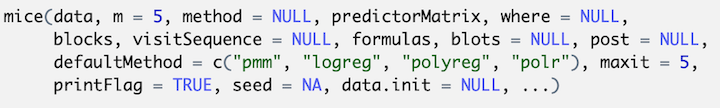
\includegraphics{figures/mice.png}
  \caption{The \texttt{mice} Function}
  \label{mice-func}
\end{figure}
\vspace{-0.5cm}

The majority of arguments are not of importance to general users. Arguments like \texttt{predictorMatrix}, which specifies the set of predictors to be used for each target column, and \texttt{blocks}, which provides the option to manually put variables into imputation blocks, require too much statistical knowledge to be of use to non-specialists. Other arguments do not affect the basic workings of the function. This applies for instance to \texttt{printFlag}, which sets the console printing preference, \texttt{seed}, which is used to offset the random number generator, and \texttt{data.init}, which specifies a data frame to be used to initialize imputations before the start of the iterative process.

The only important arguments for general users are \texttt{data}, \texttt{m}, and \texttt{defaultMethod}. Only \texttt{data} requires user input. As mentioned above, \texttt{m} should also be set to the percentage of missing data. The argument \texttt{defaultMethod} does not require user input but is crucial for insights into the default workings of \texttt{mice}. Its options \texttt{pmm}, \texttt{logreg}, \texttt{polyreg}, and \texttt{polr} refer to the default imputation methods that are implemented depending on the type of variable in question. The argument \texttt{pmm} (predictive mean matching) is used for numerical data, \texttt{logreg} (logistic regression imputation) for binary and factor data with two levels, \texttt{polyreg} (polytomous regression imputation) for factor data with more than two unordered levels, and \texttt{polr} (proportional odds model) for factor data with more than two ordered levels. Note that \texttt{mice} thus distinguishes between ordered and unordered as well as the number of factor levels, but does not specifically incorporate ordinal variables, which feature ordered but unevenly spaced levels.

\hypertarget{ordmiss-theory-multimpute-amelia}{%
\subsubsection{\texorpdfstring{\texttt{Amelia}: A Program for Missing Data}{Amelia: A Program for Missing Data}}\label{ordmiss-theory-multimpute-amelia}}

The \texttt{R} package \texttt{Amelia} was originally released in 1998 (Honaker, Joseph, King, Scheve, \& Singh, 1998). A second version, \texttt{Amelia\ II}, was released in 2010 (Honaker, King, \& Blackwell, 2012). Contrary to \texttt{mice}, which is based on IP, both versions of \texttt{Amelia} are based on the expectation-maximization (EM) algorithm (Dempster et al., 1977; Gelman et al., 2013; Jackman, 2000; McLachlan \& Krishan, 1997; Tanner, 1996). In EM, deterministic calculations of posterior means replace random draws from the entire posterior. This translates into running regressions to estimate the regression coefficient, imputing a missing value with a predicted value, re-estimating the regression coefficient, and repeating the process until convergence (King et al., 2001). While the iterations and parameters thus represent an entire density in IP, they are single maximum posterior values in EM. This makes EM comparatively much faster in finding the maximum of the likelihood function. On its own, however, EM is unsuitable for multiple imputation as it does not provide the rest of the distribution.

The \texttt{Amelia} package circumvents this issue with expectation-maximization importance sampling (EMi) (Dempster et al., 1977; Rubin, 1987), which combines EM with the iterative simulation approach of importance sampling. This proved unsuitable for large data sets, however, as it led to high running times and system crashes. The \texttt{Amelia\ II} package addresses this by mixing EM with bootstrapping (Efron, 1994; Lahlrl, 2003; Rubin, 1994; Shao \& Sitter, 1996), allowing the imputation of more variables for more observations more quickly.

\texttt{Amelia\ II} is based on the assumption that the complete data (\(\bm{X^{obs}}\) and \(\bm{X^{miss}}\)) are multivariate normal (MVN), \(\bm{X} \sim \bm{N_v}(\mu, \sum)\), with mean vector \(\mu\) and covariance matrix \(\sum\). The MVN model has been proven to work for a variety of variable types (Ezzati-Rice et al., 1995; Graham \& Schafer, 1999; Rubin \& Schenker, 1986; Schafer, 1997). Continuing the notation from section \ref{ordmiss-theory-mechanisms} and incorporating Honaker \& King (2010), let there be a vector of unknown parameters \(\bm{\theta}\), with \(\bm{\theta} = (\mu, \sum)\). Let there further be our missingness matrix \(\bm{R}\) and the likelihood of \(\bm{X^{obs}}\), \(\text{prob}(\bm{X^{obs}}, \bm{R} | \bm{\theta})\). \texttt{Amelia\ II} is explicitly set up for the MAR assumption of missing data, \(\text{prob}(\bm{R} = 0 | \bm{X^{obs}}, \bm{\theta})\). Under this assumption, the likelihood can be transformed as
\begin{align}
\text{prob}(X^{obs}, R | \theta) = \text{prob}(R | X^{obs}) \text{prob}(X^{obs} | \theta).
\end{align}
Since the missing mechanism is MAR, we are only interested in the inference on complete data parameters, thus the likelihood becomes
\begin{align}
L(\theta | X^{obs}) \propto \text{prob}(X^{obs} | \theta)
\end{align}
which further translates into
\begin{align}
\text{prob}(X^{obs} | \theta) = \int \text{prob}(X | \theta) x X^{miss}
\end{align}
under the law of iterated expectations. This results in the posterior
\begin{align}
\text{prob}(\theta | X^{obs}) \propto \text{prob}(X^{obs} | \theta) = \int \text{prob}(X | \theta) x X^{miss}.
\end{align}
Taking draws from this posterior is computationally intensive since the contents of \(\mu\) and \(\sum\) increase exponentially as the number of variables increases -- this is the perennial crux of multiple imputation, particularly for large data sets with many variables. \texttt{Amelia\ II} solves this through a combination of EM and bootstrapping. This process bootstraps the data to simulate estimation uncertainty for each posterior draw, runs the EM algorithm to find the mode of the posterior bootstrapped data, and then imputes by drawing from \(\bm{X^{miss}}\) conditional on \(\bm{X^{obs}}\) and the respective draws of \(\bm{\theta}\). The latter is a linear regression with parameters that can be estimated from \(\bm{\theta}\). This bootstrapped EM approach is faster than IP as Markov chains do not need to be assessed for convergence and an improvement over EMi since the variance matrix of \(\mu\) and \(\sum\) does not need to be calculated, allowing the algorithm to handle larger data sets.

Figure \ref{amelia-func} shows the package's main imputation function, \texttt{amelia}, with all its arguments. As stated above, I will use \texttt{amelia} with its default settings to ensure simplicity and user-friendliness.

\vspace{0.5cm}
\begin{figure}[!htbp] 
  \centering
  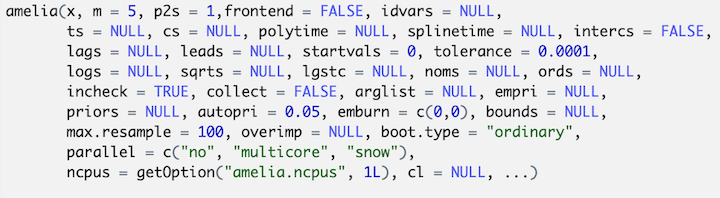
\includegraphics{figures/amelia.png}
  \caption{The \texttt{amelia} Function}
  \label{amelia-func}
\end{figure}
\vspace{-0.5cm}

As with \texttt{mice}, the majority of arguments are not of importance to general users. Specifications such as \texttt{splinetime}, which allows the control of cubic smoothing splines of time, and \texttt{lags}, which indicates columns in the data that should have their lags included in the imputation model, will only be used in very particular situations by a small minority of users. Other arguments likewise are not crucial to the basic workings of the function, such as \texttt{p2s} to control console printing and \texttt{parallel} to identify any type of parallel operation to be used.

The only argument that requires user input is \texttt{x}, which needs to be data with missing values that can be in a variety of formats. \texttt{m}, identical to \texttt{mice}, should be adjusted to reflect the percentage of missingness in the data. Three other arguments are important since they arguably comprise the core of \texttt{amelia}'s underlying imputation mechanism: \texttt{tolerance}, \texttt{autopri}, and \texttt{boot.type}. \texttt{tolerance} sets the convergence threshold for the EM algorithm. \texttt{autopri} allows the EM chain to increase the empirical prior if the path strays into an non-positive definite covariance matrix. \texttt{boot.type} offers the option to turn off the non-parametric bootstrap that is applied by default.

General multiple imputation research treats independent ordinal variables as continuous variables. \texttt{amelia} supports this and treats ordinal variables as continuous variables as a default. This means missing ordinal variables are imputed on a continuous scale, rather than preserved as the factual levels present in the observed data. However, the \texttt{ords} argument allows users to `disable' continuous ordinal imputation. In this case, ordinal variables are still imputed on a continuous scale, but these imputations are then scaled and used as the probability of success in a binomial distribution. The draw from this binomial distribution is then transformed into one of the ordinal levels present in the observed data by rounding. While \texttt{amelia} thus does incorporate ordinal variables to some extent, the rounding process changes the nature of ordinal variables to continuous variables. None of its features address or reflect the spacing between the ordinal variable categories.

\hypertarget{ordmiss-theory-multimpute-hdnorm}{%
\subsubsection{\texorpdfstring{\texttt{hot.deck}: Multiple Hot Deck Imputation}{hot.deck: Multiple Hot Deck Imputation}}\label{ordmiss-theory-multimpute-hdnorm}}

\texttt{hot.deck} is an \texttt{R} package released in 2012 (Gill \& Cranmer, 2012). It combines a variation of non-parametric hot decking (see section \ref{ordmiss-theory-singimpute}) with multiple imputation and aims to fill gaps where parametric multiple imputation, i.e.~the approach used in \texttt{mice} and \texttt{amelia}, falls short (Fuller \& Kim, 2005; Kim, 2004; Kim \& Fuller, 2004; Reilly, 1993). Like hot decking, \texttt{hot.deck} uses draws of actual observable values (\textit{donors}) to fill missing values (\textit{recipients}). In order to account for uncertainty around the drawn values, \texttt{hot.deck} iterates these draws over \(m\) imputations and pools the results.

The main proposed advantage of \texttt{hot.deck} lies in its applicability to missing data with discrete variables with a small number of categories. Approaches like the one used in \texttt{amelia}, for instance, by default impute discrete data on a continuous scale. This changes the nature of discrete variables and practically turns them into continuous variables. This can result in non-observable, biased, and sometimes even non-sensical imputation values with artificially smaller standard errors. The proposed \texttt{amelia} solution of rounding continuous imputations is problematic as well: Let imputation 1 of a binary variable between 0 and 1 be 0.4. Let further imputation 2 of the binary variable be 0.6. With rounding, these imputations become 0 and 1, when they are in fact 0.4 and 0.6. Rounding thus by definition introduces at least some level of bias. The problem is exacerbated for ordinal variables, where the spacing between the discrete variable categories is unknown, since it arbitrarily reduces or lengthens distances between the categories. This is not the case in \texttt{hot.deck} as it preserves the integrity of discrete data, does not change the size of standard errors, and produces more accurate imputations. \texttt{hot.deck} also does not require assumptions of a MVN distribution that are required by \texttt{amelia}.

Following Gill \& Cranmer (2012), \texttt{hot.deck} estimates affinity scores, \(\bm{\alpha}\), for each missing value to measure how similar a respondent with a missing value, the recipient \(c\), is to another respondent, the potential donor \(o\), across all variables except the missing one. Each score is bounded by 0 and 1. The total set of affinity scores is denoted by \(\bm{\alpha_{co}}\). For each respondent, let there be vector \((p, v)\), with \(p\) being the dependent variable and \(v\) a vector of discrete explanatory variables of length \(k\). If recipient \(c\) has \(q_c\) missing values in \(v_c\), then the potential donor vector, \(v_o\), has between 0 and \(k-q_c\) exact matches with \(c\). Let \(w_{co}\) be the number of variables where \(c\) and \(o\) have non-identical values. This leaves \(k-q_c -w_{co}\) as the number of variables where they have identical values. Scaled by the highest number of possible matches \((k-q_c)\), this value forms the affinity score
\begin{align}
\alpha_{co} = \frac{k-q_c-w_{co}}{k-q_c}
\end{align}
for each missing value recipient \(c\). When the number of identical matches decreases, so does \(\bm{\alpha_{co}}\). While this might work well for binary variables, it poses a problem for discrete variables with many levels, as the probability to find identical matches decreases. To account for this, \texttt{hot.deck} treats potential donors \(o\) for the \(h\)th variable in \(v_{o[h]}\) that are `close' differently than potential donors \(o\) that are further away. `Close' is defined as \(v_{o[h]}\) and \(v_{c[h]}\) being in the same concentric standard deviation from \(\overline{h}\), the mean of variable \(h\). Values outside of this range are penalized while values within this range are counted as matches. All donors with the highest affinity scores, i.e.~all matches, form the best imputation cell \(\bm{B}\). Since all values of \(v_{c[h]}\) in \(\bm{B}\) are part of the same distribution of independent and identically distributed (iid) random variables, which satisfies the MCAR requirement, we can use random draws from \(\bm{B}\) to impute the missing value. As with the other multiple imputation approaches, this process is then repeated \(m\) times for each missing value to account for imputation uncertainty, following the logic displayed in Figure \ref{mi-workflow}.

Figure \ref{hot.deck-func} shows the package's main imputation function, \texttt{hot.deck}, with all its arguments. As before, I will use \texttt{hot.deck} with its default settings.

\vspace{0.5cm}
\begin{figure}[!htbp] 
  \centering
  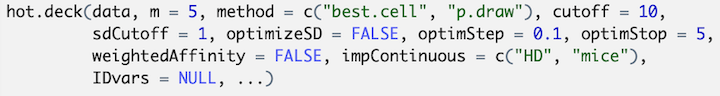
\includegraphics{figures/hot.deck.png}
  \caption{The \texttt{hot.deck} Function}
  \label{hot.deck-func}
\end{figure}
\vspace{-0.5cm}

Like \texttt{mice} and \texttt{amelia}, \texttt{hot.deck} only requires user input for \texttt{data}. \texttt{m} should once more be set to the percentage of missingness. Specialized arguments such as \texttt{optimStep} and \texttt{optimStop}, which can be tweaked to optimize standard deviation cutoff parameters, as well as \texttt{weightedAffinity}, which indicates whether a correlation-weighted affinity score should be used, do not apply to general users.

\texttt{method} and \texttt{cutoff} form the core of \texttt{hot.deck}. The default setting of \texttt{best.cell} in the \texttt{method} argument implements multiple hot deck imputation. The alternative, \texttt{p.draw}, on the other hand, merely conducts random probabilistic draws. \texttt{cutoff} allows users to specify which variables the algorithm should treat as discrete. By default, any variable up to and including 10 unique values is considered discrete. This thus includes the majority of political science survey measures, with the sensible exceptions of variables like age or for instance widely spread assessments of income levels.

Overall, \texttt{hot.deck} is a specialized function to improve the application of multiple imputation for discrete data and has been shown to do so for highly granular discrete data (Gill \& Cranmer, 2012). Moreover, political science survey research relies on highly discrete measures. What is missing from \texttt{hot.deck}, however, is the incorporation of ordinal variables as a special form of discrete data. I thus identify this gap as a leverage point to improve the use of ordinal variables in the imputation of missing data. To do so, I adapt \texttt{hot.deck} to form \texttt{hd.ord}, a function specifically designed to utilize the ordered but unevenly spaced information contained in ordinal variables.

\hypertarget{ordmiss-theory-multimpute-hdord}{%
\subsubsection{\texorpdfstring{\texttt{hd.ord}: Multiple Hot Deck Imputation with Ordinal Variables}{hd.ord: Multiple Hot Deck Imputation with Ordinal Variables}}\label{ordmiss-theory-multimpute-hdord}}

\texttt{hd.ord} is a self-penned \texttt{R} function designed specifically to implement multiple hot deck imputation with ordinal variables. It is an extension of \texttt{hot.deck} and fully utilizes the unevenly spaced yet ordered information contained in ordinal variables. As described in section \ref{ordblock-theory-op}, ordinal variables matter in political science surveys because a key variable in such surveys is ordinal: education. The importance of the spacing between education values is best demonstrated with a simplified example shown in Table \ref{ordmiss-ordspace}.
\begin{table}[!htbp] 
  \centering
  \caption{Illustrative Data}
  \label{ordmiss-ordspace}
  \begin{tabular}{lccccc}
  \bottomrule 
  \midrule
  Respondent & Age & Party ID & Education & Income & Gender\\
  \hline
  A & 25 & Republican & High School Graduate & \$30-40,000 & Male \\
  B & 40 & NA & Some High School &  \$20-30,000 & Female\\
  C & 30 & Democrat & Bachelor's Degree &  \$50-60,000 & Female\\
  \bottomrule 
  \end{tabular}
\end{table}
Respondent B shows missing data for party ID. To impute a fill-in value, we look at how close respondents A and C are to B in terms of age, education, income, and gender. C is closer to B in terms of age and they share the same gender. A is closer to B on education and income. \texttt{hot.deck} measures these distances and estimates affinity scores for respondents A and C. The affinity scores measure how close A and C are to B on all variables except the missing one, i.e.~party ID. B then receives the party ID fill-in value from whichever respondent has the higher score. The algorithm building the affinity score is based on evenly spaced sequential numerical values, e.g.~1, 2, 3 etc. to represent the distances between the variable categories. This makes sense for age, income, and gender, but not for education, since education is an ordinal variable. Applying \texttt{hot.deck} to such a numerical representation might thus misrepresent the data.

To avoid this, \texttt{hd.ord} uses the ordered probit approach described in section \ref{ordblock-theory-op}. It applies \texttt{polr} from the \texttt{MASS} package to any specified number of ordinal variables in the data to estimate the underlying latent continuous variable. This estimates cutoff thresholds between the ordinal categories and bins data cases according to the linear predictors. The binned cases determine which variable categories make sense, given the underlying latent continuous variable. This can result in a reduction of education categories if the categories are too finely thinned out. \texttt{hd.ord} estimates the mid-cutpoints between each of these newly estimated categories based on the \texttt{polr} results. We then replace the ordinal variable categories with the newly estimated numerical mid-cutpoints in the data. Finally, these values are scaled and used to assess distances to calculate affinity scores.

Table \ref{ordmiss-ill-res} illustrates this procedure with results from running \texttt{polr} on rudimentary survey data, with column ``Thresholds'' showing the estimated cutoff thresholds between the education categories. Table \ref{ordmiss-ill-mid} in turn shows the estimated mid-cutpoints for each of the education categories. The mid-cutpoint values for the categories in Table \ref{ordmiss-ill-mid} fall between the adjacent values in Table \ref{ordmiss-ill-res}, i.e.~the mid-cutpoint of 2.956 for ``Some High School'' lies between the respective thresholds of 2.418 and 3.495. To estimate the beginning cutpoint for the first category (``Less Than High School''), we halve the difference between the first and second threshold and subtract this value from the first threshold: 2.418 \(-\) (3.495 \(-\) 2.418) / 2 = 1.88. The same process is applied to estimate the ending cutpoint for the last category (``Master's Degree''). The mid-cutpoint values are then scaled and used for the calculation of the affinity scores.
\begin{table}[!htbp] \centering 
  \caption{Illustrative Data `polr` Results} 
  \label{ordmiss-ill-res} 
\begin{tabular}{r@{}lr@{}l} 
\\[-1.8ex]\hline 
\hline \\[-1.8ex] 
\multicolumn{2}{c}{Intercepts} & \multicolumn{2}{c}{Thresholds} \\ 
\hline \\[-1.8ex] 
Less Than High School $\mid$ & \,Some High School & 2.&418 \\ 
Some High School $\mid$ & \,High School Graduate & 3.&495 \\ 
High School Graduate $\mid$ & \,Some College & 4.&214 \\ 
Some College $\mid$ & \,Bachelor's Degree & 5.&727 \\ 
Bachelor's Degree $\mid$ & \,Master's Degree & 7.&412 \\ 
\hline \\[-1.8ex] 
\end{tabular} 
\end{table}
\begin{table}[!htbp] \centering 
  \caption{Illustrative Data Value Replacements} 
  \label{ordmiss-ill-mid} 
\begin{tabular}{@{\extracolsep{5pt}} D{.}{.}{-3} D{.}{.}{-3} } 
\\[-1.8ex]\hline 
\hline \\[-1.8ex] 
\multicolumn{1}{c}{Original Education Categories} & \multicolumn{1}{c}{Mid-Cutpoints} \\ 
\hline \\[-1.8ex] 
\multicolumn{1}{c}{Less Than High School} & 1.879 \\ 
\multicolumn{1}{c}{Some High School} & 2.956 \\ 
\multicolumn{1}{c}{High School Graduate} & 3.854 \\ 
\multicolumn{1}{c}{Some College} & 4.970 \\ 
\multicolumn{1}{c}{Bachelor's Degree} & 6.569 \\ 
\multicolumn{1}{c}{Master's Degree} & 8.254 \\ 
\hline \\[-1.8ex] 
\end{tabular} 
\end{table}
Figure \ref{hd.ord-func} shows \texttt{hd.ord} with all its arguments. As before, I will use \texttt{hd.ord} with its default settings. Since \texttt{hd.ord} is an adaptation of \texttt{hot.deck}, the two functions are identical except for the \texttt{ord} argument, which allows users to specify the ordinal variables for \texttt{polr} treatment.

\vspace{0.5cm}
\begin{figure}[!htbp]
  \centering
  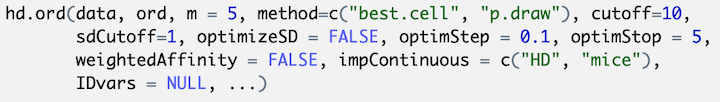
\includegraphics{figures/hd.ord.png}
  \caption{The \texttt{hd.ord} Function}
  \label{hd.ord-func}
\end{figure}
\vspace{-0.5cm}

\hypertarget{ordmiss-data}{%
\section{Data}\label{ordmiss-data}}

To test the performance of imputation methods, we need to work with complete data, as only complete data allow us to obtain the true values needed as a benchmark for comparison. I choose two different sets of survey data from the 2016 ANES and the 2016 CCES. Data for all selected variables in both data sets is complete. In order to test the accuracy of several imputation methods, I delete data from these complete data sets with the \texttt{ampute} function from the \texttt{mice} package (Buuren et al., 2020). \texttt{ampute} allows the removal of data MCAR, MAR, and MNAR. Particularly the availability of the latter offers unique opportunities, as it can be a difficult feat to establish whether real-life missing data is MNAR. Data that are artificially created to be MNAR, however, circumvent this problem and allow us to test the accuracy of imputation methods for this type of missing data as well. \texttt{ampute} has been shown to accurately remove data MCAR, MAR, and MNAR (Schouten, Lugtig, \& Vink, 2018).

Each data set is imputed with four different \texttt{R} functions: \texttt{hd.ord}, \texttt{hot.deck}, \texttt{amelia}, and \texttt{mice}. I also apply list-wise deletion with \texttt{na.omit}. As outlined in section \ref{ordmiss-theory-multimpute}, all functions are used with their default settings but with the number of imputations set to the percentage of missingness.

I test each function for accuracy and speed for binary, ordinal, and interval variables in both data sets. Each data set contains two ordinal (\texttt{Education}, \texttt{Interest}), two interval (\texttt{Age}, \texttt{Income}) and numerous binary variables. In order to enable factually accurate comparison and unless explicitly specified otherwise, each data set contains 1,000 observations and six levels of the ordinal variable \texttt{Education}. 1,000 observations represent a common size for survey and survey experiment data, and the \texttt{polr} analysis from section \ref{ordblock-data} estimates five or six levels to best represent \texttt{Education} in a US context. Each data set was imputed 1,000 times with each of the four imputation methods. With the exception of Figure \ref{accuracy50} and Table \ref{run.cces.perc}, 20 percent missing data were randomly amputed in each iteration for each data set.\footnote{The decision to reduce the number of education categories in the ANES data is made out of necessity. It is not feasible to use all ANES observations, as repeated multiple imputation is computationally intensive for a sample of this size. The reduction to 1,000 observations in turn makes it impossible to use all original categories, since the insertion of missing data would consistently lead to dropped categories, which in turn would render a comparison of imputation runs pointless. See appendix section \ref{app-ordmiss-allObs} for imputations for all ANES and CCES observations (as much as computationally possible).}

Following Collins et al. (2001) and Honaker \& King (2010), as many relevant observed variables as possible were used to impute each of the data sets. For the ANES data, up to 14 predictor variables were used: \texttt{Independent}, \texttt{Moderate}, \texttt{Black}, \texttt{Hispanic}, \texttt{Asian}, \texttt{Employed}, \texttt{Student}, \texttt{Religious}, \texttt{InternetHome}, \texttt{OwnHome}, \texttt{Rally} (have you attended a political rally), \texttt{Donate} (have you donated to a political candidate), \texttt{Married}, and \texttt{Separated}. For the CCES data, up to 17 predictor variables were used: \texttt{Republican}, \texttt{Moderate}, \texttt{Liberal}, \texttt{Black}, \texttt{Hispanic}, \texttt{Asian}, \texttt{Employed}, \texttt{Unemployed}, \texttt{Student}, \texttt{Gay}, \texttt{Bisexual}, \texttt{StudLoans} (do you have student loans), \texttt{InternetHome}, \texttt{NotReligious}, \texttt{RentHome}, \texttt{Separated}, and \texttt{Single}. Highly collinear variables were excluded with a cutoff of 0.6.

The variable mean serves as the baseline of comparison for the performance of each imputation method. Since each data set is complete, we know the true variable mean of all variables. The closer a method comes to the true mean, the better its performance. I impute both data sets for data MAR and MNAR for five amputed variables: \texttt{Democrat} (binary), \texttt{Male} (binary), \texttt{Interest} (ordinal, scaled from 1 to 4), \texttt{Income} (interval), and \texttt{Age} (interval). Imputation is not necessary for data MCAR because simple deletion leads to unbiased and therefore valid results. I subsequently increase the number of ordinal variables to be treated by \texttt{polr} in \texttt{hd.ord} by including \texttt{Interest}. Imputations are again conducted MAR and MNAR, this time for four amputed variables. The amputed variables are the same as before but omitting \texttt{Interest}. Next, I test the effect of increasing the amount of missing data to 50 percent. Finally, I compare the imputation runtimes for each method.

\hypertarget{ordmiss-results}{%
\section{Results}\label{ordmiss-results}}

\hypertarget{ordmiss-results-mar}{%
\subsection{MAR}\label{ordmiss-results-mar}}

This section shows the imputation results for the MAR missing data mechanism. MAR amputation was achieved by setting the \texttt{mech} argument in the \texttt{ampute} function to \texttt{MAR}. Table \ref{mar.5var} shows the results of imputing both data sets MAR for five amputed variables. For the two binary variables, \texttt{Democrat} and \texttt{Male}, \texttt{hd.ord} performs on par or worse than \texttt{hot.deck} for both data sets, while \texttt{mice} and \texttt{amelia} perform best. \texttt{hd.ord} is relatively close for CCES \texttt{Democrat} (+0.0001 \texttt{amelia} vs.~+0.0000 \texttt{hd.ord}) but further away for ANES ( +0.0003 \texttt{mice} vs.~--0.0010 \texttt{hd.ord} \texttt{Democrat}; +0.0001 \texttt{mice} vs.~--0.0013 \texttt{hd.ord} \texttt{Male}) and CCES \texttt{Male} (--0.0001 \texttt{amelia} vs.~--0.0011 \texttt{hd.ord}).
\begin{table}[!htbp] \centering   
 \caption{Accuracy of Multiple Imputation Methods. ANES and CCES Data, MAR, 5 Variables with NA}   
 \label{mar.5var}  
\begin{threeparttable}
 \begin{tabular}{ccr@{}lr@{}l}  
 \\[-1.8ex]\hline 
 \hline \\[-1.8ex]  
 \multicolumn{1}{c}{Method} & \multicolumn{1}{c}{Variable} & \multicolumn{2}{c}{ANES} & \multicolumn{2}{c}{CCES} \\
 \hline \\[-1.8ex]  
 true & Democrat & 0.&3420 & 0.&3770 \\
 hd.ord & Democrat & --0.&0010 & +0.&0000 \\ 
 hot.deck & Democrat & --0.&0011 & --0.&0004 \\ 
 amelia & Democrat & +0.&0004 & +0.&0001 \\
 mice & Democrat & +0.&0003 & +0.&0002 \\
 na.omit & Democrat & --0.&0290 & --0.&0229 \\
 true & Male & 0.&4890 & 0.&4830 \\
 hd.ord & Male & --0.&0013 & --0.&0011 \\
 hot.deck & Male & --0.&0013 & --0.&0014 \\
 amelia & Male & +0.&0002 & --0.&0001 \\
 mice & Male & +0.&0001 & --0.&0001 \\
 na.omit & Male & --0.&0392 & --0.&0414 \\
 true & Interest & 2.&9340 & 3.&3290 \\
 hd.ord & Interest & --0.&0130 & --0.&0125 \\
 hot.deck & Interest & --0.&0191 & --0.&0196 \\ 
 amelia & Interest & +0.&0003 & +0.&0003 \\ 
 mice & Interest & +0.&0003 & +0.&0000 \\
 na.omit & Interest & --0.&0705 & --0.&0724 \\
 true & Income & 16.&6140 & 6.&4810 \\
 hd.ord & Income & --0.&1068 & --0.&0259 \\
 hot.deck & Income & --0.&1278 & --0.&0407 \\
 amelia & Income & +0.&0008 & --0.&0004 \\
 mice & Income & +0.&0003 & --0.&0002 \\
 na.omit & Income & --0.&5631 & --0.&2468 \\
 true & Age & 50.&0410 & 52.&8230 \\
 hd.ord & Age & --0.&3888 & --0.&2616 \\
 hot.deck & Age & --0.&4597 & --0.&3895 \\
 amelia & Age & +0.&0007 & --0.&0033 \\
 mice & Age & +0.&0017 & --0.&0073 \\
 na.omit & Age & --1.&1875 & --1.&2361 \\
 \hline \\[-1.8ex]  
\end{tabular} 
\begin{tablenotes}[para,flushleft]
\footnotesize{\textit{Note:} Each \texttt{true} value shows the true variable mean. All other values show the differences between the imputation means and the true mean, indicated with a + or -- sign.}
\end{tablenotes}
\end{threeparttable}
\end{table}
For the ordinal variable, \texttt{Interest}, \texttt{hd.ord} performs worst for both data sets, with considerable distance to \texttt{hot.deck} (--0.0130 vs.~--0.0191 ANES; --0.0125 vs.~--0.0196 CCES). \texttt{mice} and \texttt{amelia} perform by far best across both data sets. The performance differences between the methods are far larger for the ordinal than for the binary variables: \texttt{mice} is not more than +0.0003 (ANES) away from the true value across both data sets, while the maximum difference for \texttt{hd.ord} amounts to --0.0130 (ANES).

For the interval variables, \texttt{Income} and \texttt{Age}, \texttt{hd.ord} also performs worst for both data sets. The distance to \texttt{hot.deck} is once more considerable. \texttt{mice} performs best for \texttt{Income} and \texttt{amelia} shows the best results for \texttt{Age}. The performance differences between the methods are even larger here: For \texttt{Income}, \texttt{mice} is not more than --0.0002 (CCES) away from the true value across both data sets, but the maximum difference for \texttt{hd.ord} is --0.1068 (ANES). Similarly, \texttt{amelia}'s largest deviation from the true value for \texttt{Age} is --0.0033 (CCES) as opposed to \texttt{hd.ord}'s --0.3888 (ANES).\footnote{For a repeat of this MAR analysis for 12 amputed variables, see appendix section \ref{app-ordmiss-12var}. The results do not change substantively.}

\hypertarget{ordmiss-results-mnar}{%
\subsection{MNAR}\label{ordmiss-results-mnar}}

This section shows the imputation results for the MNAR missing data mechanism. MNAR amputation was achieved by setting the \texttt{mech} argument in the \texttt{ampute} function to \texttt{MNAR}. All MAR and MNAR analyses are otherwise identical. Table \ref{mnar.5var} shows the results of imputing both data sets MNAR for five amputed variables. It is immediately noticeable that the differences between the methods' imputation results and the true values are much higher for all methods for all variables for both data sets. The results for \texttt{Democrat} and \texttt{Male}, for instance, hover around 0.0100 and 0.0125 for both data sets. In the corresponding MAR analysis, however, the results for \texttt{Democrat} and \texttt{Male} showed around 0.0005.
\begin{table}[!htbp] \centering 
 \caption{Accuracy of Multiple Imputation Methods. ANES and CCES Data, MNAR, 5 Variables with NA}  
 \label{mnar.5var} 
\begin{threeparttable}
 \begin{tabular}{ccr@{}lr@{}l} 
 \\[-1.8ex]\hline 
 \hline \\[-1.8ex]  
 \multicolumn{1}{c}{Method} & \multicolumn{1}{c}{Variable} & \multicolumn{2}{c}{ANES} & \multicolumn{2}{c}{CCES} \\
 \hline \\[-1.8ex]  
 true & Democrat & 0.&3420 & 0.&3770 \\
 hd.ord & Democrat & --0.&0114 & --0.&0099 \\ 
 hot.deck & Democrat & --0.&0120 & --0.&0105 \\
 amelia & Democrat & --0.&0106 & --0.&0102 \\
 mice & Democrat & --0.&0099 & --0.&0101 \\ 
 na.omit & Democrat & --0.&0176 & --0.&0140 \\
 true & Male & 0.&4890 & 0.&4830 \\ 
 hd.ord & Male & --0.&0136 & --0.&0116 \\ 
 hot.deck & Male & --0.&0133 & --0.&0124 \\
 amelia & Male & --0.&0132 & --0.&0121 \\
 mice & Male & --0.&0132 & --0.&0120 \\
 na.omit & Male & --0.&0214 & --0.&0219 \\
 true & Interest & 2.&9340 & 3.&3290 \\ 
 hd.ord & Interest & --0.&0288 & --0.&0246 \\ 
 hot.deck & Interest & --0.&0335 & --0.&0296 \\
 amelia & Interest & --0.&0167 & --0.&0146 \\
 mice & Interest & --0.&0167 & --0.&0146 \\
 na.omit & Interest & --0.&0379 & --0.&0372 \\
 true & Income & 16.&6140 & 6.&4810 \\
 hd.ord & Income & --0.&2299 & --0.&0928 \\ 
 hot.deck & Income & --0.&2554 & --0.&1038 \\
 amelia & Income & --0.&1225 & --0.&0578 \\
 mice & Income & --0.&1229 & --0.&0566 \\
 na.omit & Income & --0.&2770 & --0.&1334 \\
 true & Age & 50.&0410 & 52.&8230 \\
 hd.ord & Age & --0.&6319 & --0.&4596 \\ 
 hot.deck & Age & --0.&7415 & --0.&5929 \\ 
 amelia & Age & --0.&2450 & --0.&2266 \\
 mice & Age & --0.&2369 & --0.&2160 \\ 
 na.omit & Age & --0.&6427 & --0.&6392 \\
 \hline \\[-1.8ex] 
\end{tabular} 
\begin{tablenotes}[para,flushleft]
\footnotesize{\textit{Note:} Each \texttt{true} value shows the true variable mean. All other values show the differences between the imputation means and the true mean, indicated with a + or -- sign.}
\end{tablenotes}
\end{threeparttable}
\end{table}
For the binary variables, \texttt{hd.ord} performs more closely on par with \texttt{amelia} and \texttt{mice} than in the corresponding MAR analysis above, sometimes more (--0.0136 \texttt{hd.ord} vs.~--0.0132 \texttt{amelia} ANES \texttt{Male}) and sometimes less so (--0.0114 \texttt{hd.ord} vs.~--0.0099 \texttt{mice} ANES \texttt{Democrat}). The results for the ordinal variables confirm those of the MAR analysis: \texttt{hd.ord} represents the worst method across both data sets. \texttt{amelia} and \texttt{mice} show by far the best results and are virtually identical with each other, though the differences to the true values are much higher than in the MAR analysis, as is the case for the entire MNAR analysis. The results for the interval variables paint the same picture as the ordinal ones. \texttt{hd.ord} shows the worst performance. Note that \texttt{na.omit} performs equally well as \texttt{hd.ord} for ANES \texttt{Age}.\footnote{For a repeat of this MNAR analysis for 12 amputed variables, see appendix section \ref{app-ordmiss-12var}. The results do not change substantively.}

\hypertarget{ordmiss-results-increaseOrd}{%
\subsection{Increased Number of Ordinal Variables}\label{ordmiss-results-increaseOrd}}

This section shows the imputation results for an increased number of ordinal variables to be treated by \texttt{polr} in \texttt{hd.ord}. Specifically, I add \texttt{Interest} to the \texttt{ord} argument in \texttt{hd.ord}. The intuition behind this is a strengthening of the underlying latent continuous variable assumption. The results of the previous analyses do not show superior performance by \texttt{hd.ord}, but perhaps this might be due to a lack of `influence' so far. Perhaps one ordinal variable treated with \texttt{polr} is not enough to manifest itself in improved results. By including another ordinal variable in the treatment, this `influence' is strengthened and the \texttt{polr} assumption is put to another test. As in sections \ref{ordmiss-results-mar} and \ref{ordmiss-results-mnar}, imputations are conducted MAR and MNAR. Because \texttt{Interest} `moves' to the \texttt{polr} treatment, the number of imputed variables is reduced to four and 11, respectively, to ensure accurate comparison. This means the amputed variables do not include an ordinal variable any more. The remaining variables are the same as before.

Table \ref{mult.mar.4var} shows the results of imputing both data sets with two \texttt{polr}-treated variables MAR for four amputed variables. \texttt{hd.ord} displays the worst results for \texttt{Democrat} across both data sets and beats only \texttt{hot.deck} for \texttt{Male}. \texttt{amelia} and \texttt{mice} perform best and show virtually identically results that often match the true variable means. A comparison with the MAR analysis of five imputed variables reveals that \texttt{hd.ord} consistently performs slightly worse here: --0.0008 and +0.0002 vs.~--0.0010 and +0.0000 for \texttt{Democrat}; --0.0022 and --0.0019 vs.~--0.0013and --0.0011 for \texttt{Male}.
\begin{table}[!htbp] \centering  
 \caption{Accuracy of Multiple Imputation Methods. ANES and CCES Data, 2 Ordinal Variables (Education, Interest), MAR, 4 Variables with NA} 
 \label{mult.mar.4var} 
\begin{threeparttable}
 \begin{tabular}{ccr@{}lr@{}l} 
 \\[-1.8ex]\hline 
 \hline \\[-1.8ex] 
 \multicolumn{1}{c}{Method} & \multicolumn{1}{c}{Variable} & \multicolumn{2}{c}{ANES} & \multicolumn{2}{c}{CCES} \\
 \hline \\[-1.8ex]
 true & Democrat & 0.&3420 & 0.&3770 \\
 hd.ord & Democrat & --0.&0008 & +0.&0002 \\
 hot.deck & Democrat & --0.&0018 & --0.&0005 \\
 amelia & Democrat & +0.&0002 & +0.&0001 \\
 mice & Democrat & +0.&0001 & +0.&0002 \\
 ha.omit & Democrat & --0.&0333 & --0.&0294 \\
 true & Male & 0.&4890 & 0.&4830 \\
 hd.ord & Male & --0.&0022 & --0.&0019 \\
 hot.deck & Male & --0.&0015 & --0.&0018 \\
 amelia & Male & +0.&0001 & +0.&0000 \\
 mice & Male & +0.&0000 & +0.&0000 \\ 
 ha.omit & Male & --0.&0396 & --0.&0407 \\
 true & Income & 16.&6140 & 6.&4810 \\
 hd.ord & Income & --0.&0830 & --0.&0246 \\
 hot.deck & Income & --0.&1523 & --0.&0516 \\
 amelia & Income & +0.&0010 & --0.&0006 \\
 mice & Income & --0.&0008 & +0.&0002 \\
 ha.omit & Income & --0.&5771 & --0.&2564 \\
 true & Age & 50.&0410 & 52.&8230 \\
 hd.ord & Age & --0.&2889 & --0.&2350 \\
 hot.deck & Age & --0.&5431 & --0.&4664 \\
 amelia & Age & +0.&0018 & +0.&0085 \\
 mice & Age & +0.&0024 & --0.&0002 \\ 
 ha.omit & Age & --1.&1521 & --1.&1228 \\
 \hline \\[-1.8ex] 
\end{tabular} 
\begin{tablenotes}[para,flushleft]
\footnotesize{\textit{Note:} Each \texttt{true} value shows the true variable mean. All other values show the differences between the imputation means and the true mean, indicated with a + or -- sign.}
\end{tablenotes}
\end{threeparttable}
\end{table}
\texttt{hd.ord} also performs worst for both data sets across both interval variables. \texttt{amelia} and \texttt{mice} again perform best. \texttt{amelia} and \texttt{mice} perform equally well for ANES, while \texttt{mice} does better for CCES. As for the binary variables, the results for \texttt{hd.ord} consistently get slightly worse in the switch from one to two ordinal variables in \texttt{polr}-treatment: --0.0830 and --0.0246 vs.~--0.1068 and --0.0259 for \texttt{Income}; --0.2889 and --0.2350 vs.~--0.3888 and --0.2616 for \texttt{Age}.\footnote{For a repeat of this MAR analysis for 11 amputed variables and two ordinal variables, see appendix section \ref{app-ordmiss-mult-11var}. The results do not change substantively.}

Table \ref{mult.mnar.4var} shows the results of imputing both data sets with two \texttt{polr}-treated variables MNAR for four amputed variables. For the binary variables, \texttt{hd.ord} performs on the same level as \texttt{amelia} and \texttt{mice} when compared to the MNAR analysis of five imputed variables with only \texttt{Education} treated by \texttt{polr}; sometimes more (--0.0133 \texttt{hd.ord} vs.~--0.0130 \texttt{mice} CCES \texttt{Democrat}), sometimes less so (--0.0142 \texttt{hd.ord} vs.~--0.0127 \texttt{mice} ANES \texttt{Democrat}). \texttt{na.omit} does not perform as well as it does in Table \ref{mnar.5var}. \texttt{hd.ord} again consistently performs slightly worse with the two-ordinal-variable-\texttt{polr}-treatment: --0.0142 and --0.0133 vs.~--0.0114 and --0.0099 for \texttt{Democrat}; --0.0180 and --0.0162 vs.~--0.0136 and --0.0116 for \texttt{Male}.
\begin{table}[!htbp] \centering
 \caption{Accuracy of Multiple Imputation Methods. ANES and CCES Data, 2 Ordinal Variables (Education, Interest), MNAR, 4 Variables with NA} 
 \label{mult.mnar.4var} 
\begin{threeparttable}
 \begin{tabular}{ccr@{}lr@{}l} 
 \\[-1.8ex]\hline  
 \hline \\[-1.8ex]
 \multicolumn{1}{c}{Method} & \multicolumn{1}{c}{Variable} & \multicolumn{2}{c}{ANES} & \multicolumn{2}{c}{CCES} \\
 \hline \\[-1.8ex] 
 true & Democrat & 0.&3420 & 0.&3770 \\ 
 hd.ord & Democrat & --0.&0142 & --0.&0133 \\ 
 hot.deck & Democrat & --0.&0155 & --0.&0131 \\
 amelia & Democrat & --0.&0136 & --0.&0131 \\
 mice & Democrat & --0.&0127 & --0.&0130 \\
 na.omit & Democrat & --0.&0211 & --0.&0185 \\
 true & Male & 0.&4890 & 0.&4830 \\
 hd.ord & Male & --0.&0180 & --0.&0162 \\
 hot.deck & Male & --0.&0172 & --0.&0160 \\
 amelia & Male & --0.&0170 & --0.&0154 \\
 mice & Male & --0.&0170 & --0.&0153 \\ 
 na.omit & Male & --0.&0233 & --0.&0241 \\
 true & Income & 16.&6140 & 6.&4810 \\
 hd.ord & Income & --0.&2481 & --0.&1034 \\ 
 hot.deck & Income & --0.&3174 & --0.&1303 \\
 amelia & Income & --0.&1555 & --0.&0741 \\
 mice & Income & --0.&1568 & --0.&0730 \\
 na.omit & Income & --0.&3114 & --0.&1513 \\
 true & Age & 50.&0410 & 52.&8230 \\
 hd.ord & Age & --0.&6020 & --0.&4844 \\
 hot.deck & Age & --0.&8997 & --0.&7259 \\
 amelia & Age & --0.&3103 & --0.&2831 \\
 mice & Age & --0.&2994 & --0.&2702 \\
 na.omit & Age & --0.&6726 & --0.&6482 \\
 \hline \\[-1.8ex] 
\end{tabular} 
\begin{tablenotes}[para,flushleft]
\footnotesize{\textit{Note:} Each \texttt{true} value shows the true variable mean. All other values show the differences between the imputation means and the true mean, indicated with a + or -- sign.}
\end{tablenotes}
\end{threeparttable}
\end{table}
The results for the interval variables are consistent with the previous analyses. In addition, note that \texttt{na.omit} performs better than \texttt{hd.ord} for \texttt{Age} in both data sets and for ANES \texttt{Income}. Once more, \texttt{hd.ord} consistently performs slightly worse with more than two ordinal variables: --0.2481 and --0.1034 vs.~--0.2299 and --0.0928 for \texttt{Income}; --0.6020 and --0.4844 vs.~--0.6319 and --0.4596 for \texttt{Age}.\footnote{For a repeat of this MNAR analysis for 11 amputed variables and two ordinal variables, see appendix section \ref{app-ordmiss-mult-11var}. The results do not change substantively.}

\clearpage

\hypertarget{ordmiss-results-increaseNA}{%
\subsection{Increased Percentage of Missingness}\label{ordmiss-results-increaseNA}}

This brief section shows the imputation results when the percentage of missingness is increased. I conduct this for data MAR for five variables with the CCES data. Figures \ref{accuracy20} and \ref{accuracy50} show the results for 20 and 50 percent missingness, respectively.
\begin{figure}
\centering
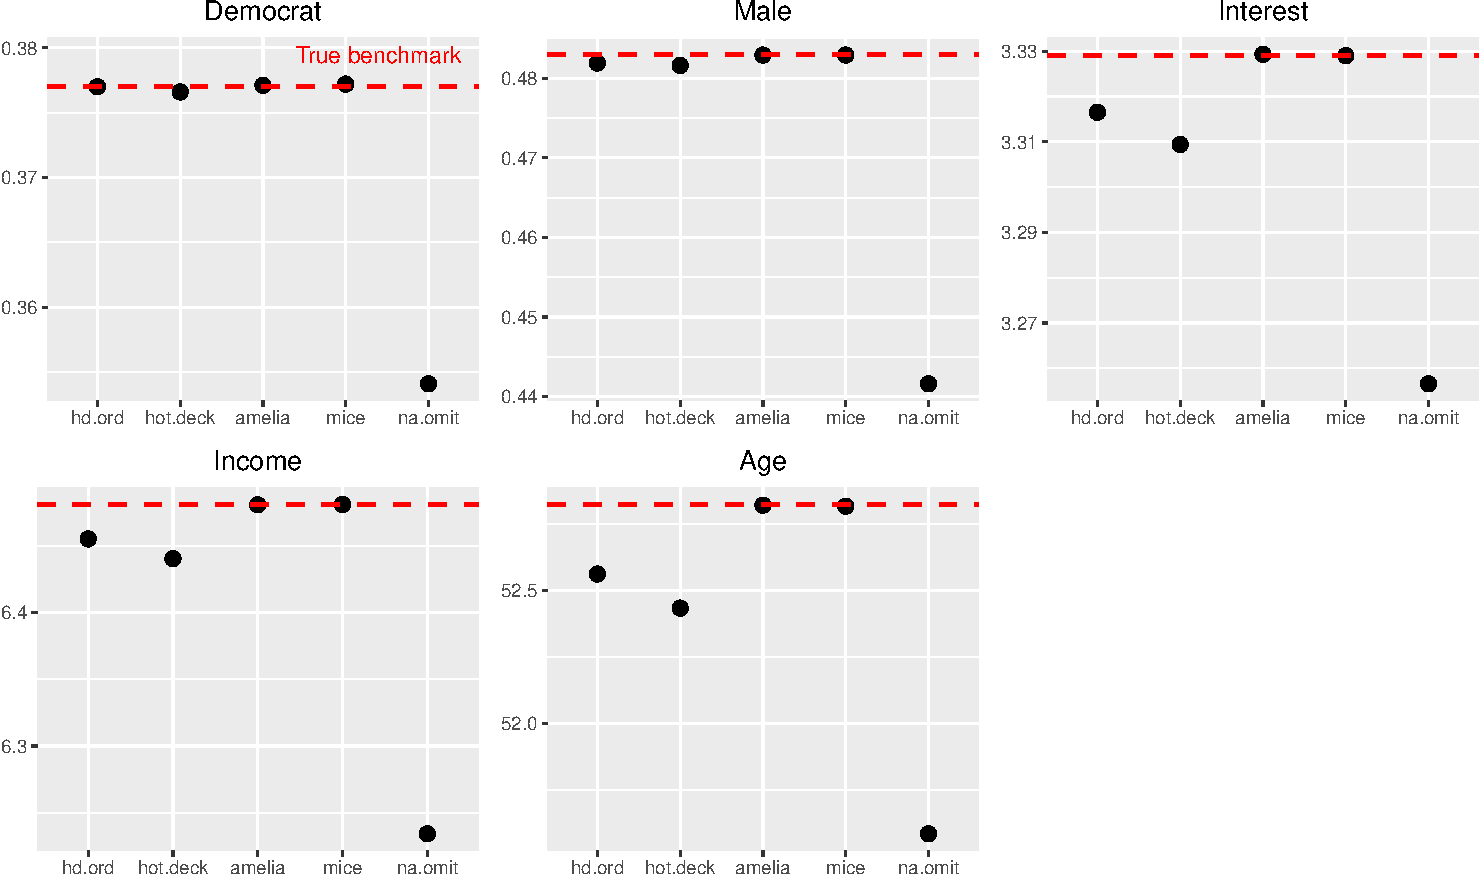
\includegraphics{dissertation_files/figure-latex/Increased-Missingness-20-Percent-1.pdf}
\caption{\label{fig:Increased-Missingness-20-Percent}Accuracy of Multiple Imputation Methods for 20 Percent Missingness. CCES Data, MAR, Five Variables with NA. Y-Axis Shows Percentages/Means.\label{accuracy20}}
\end{figure}
\begin{figure}
\centering
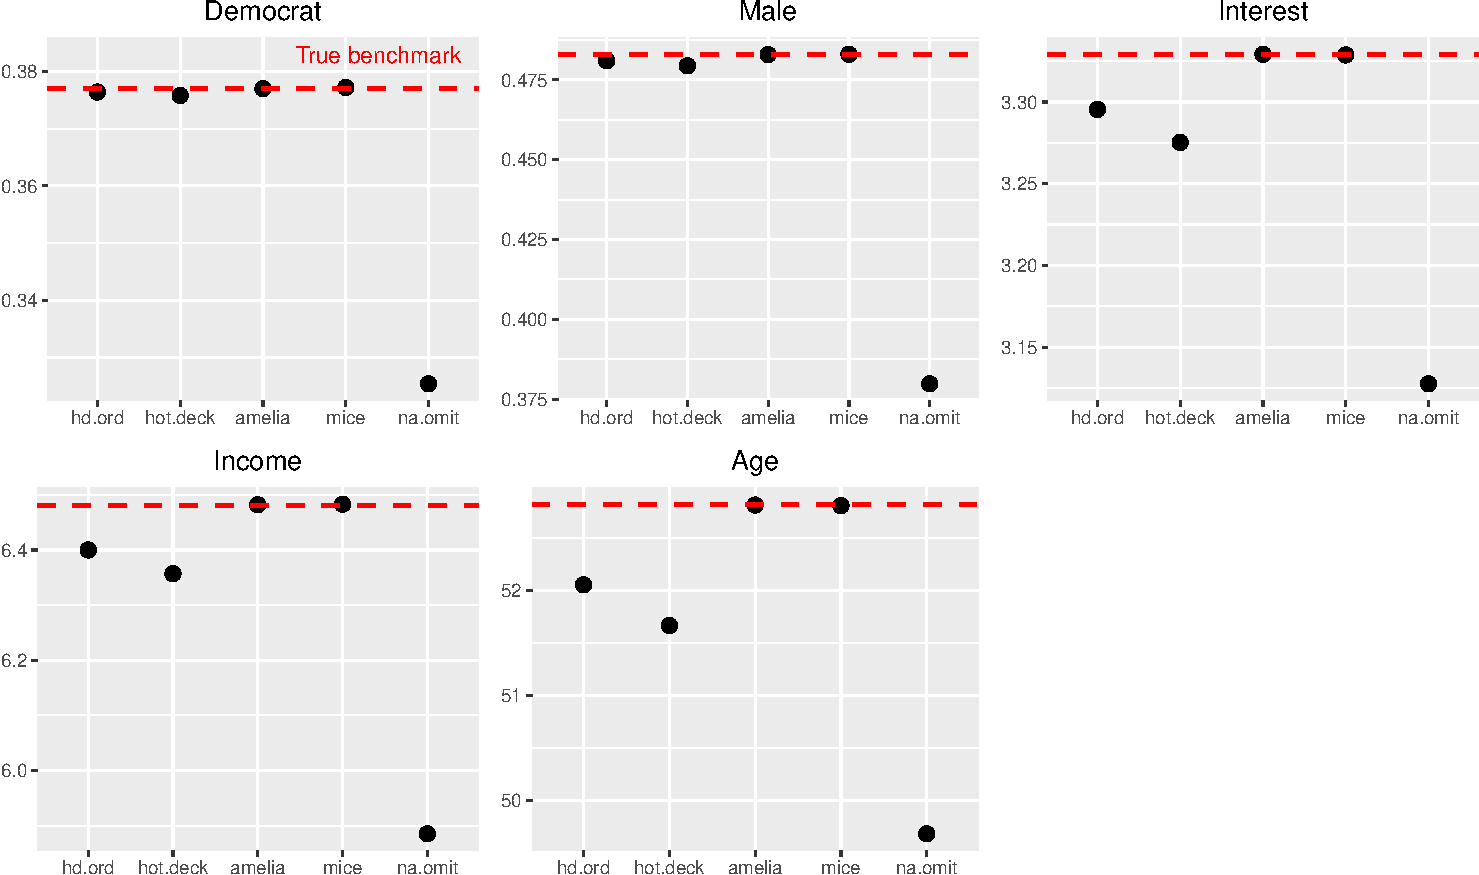
\includegraphics{dissertation_files/figure-latex/Increased-Missingness-50-Percent-1.pdf}
\caption{\label{fig:Increased-Missingness-50-Percent}Accuracy of Multiple Imputation Methods for 50 Percent Missingness. CCES Data, MAR, Five Variables with NA. Y-Axis Shows Percentages/Means.\label{accuracy50}}
\end{figure}
\texttt{hd.ord} performs comparatively well for 50 percent missing data \texttt{Democrat} (--0.0006 vs.~+0.0000 \texttt{amelia}) but falls short for \texttt{Male} (--0.0020 vs.~+0.0000 \texttt{mice}). \texttt{hd.ord} also represents the second-worst imputation method for both percentages for the ordinal and interval variables. \texttt{amelia} and \texttt{mice} show virtually identical results, are hardly affected by the increase in missingness, and far outperform the other methods.

\hypertarget{ordmiss-results-speed}{%
\subsection{Speed}\label{ordmiss-results-speed}}

This section shows the running times for all methods. I outline the speed differences for both data sets (Table \ref{runtimes5var}) and by the percentage of missingness for the CCES data (Table \ref{run.cces.perc}). Both analyses are conducted MAR for five imputed variables. All running times are given in minutes, apply to all 1,000 imputation iterations combined, and were achieved on a Code Ocean AWS EC2 instance with 16 cores and 120 GB of memory.

Table \ref{runtimes5var} shows \texttt{hd.ord} and \texttt{hot.deck} with virtually identical running times for both data sets. This is to be expected as both methods are very similar in terms of their code build-up. More importantly, however, we observe that both methods are much faster than \texttt{amelia} and \texttt{mice}: \texttt{amelia} is 3.4 times slower than \texttt{hd.ord} for the ANES data and 3.8 times slower for the CCES data. \texttt{mice}, however, is by far the slowest method and takes 20.6 (CCES) and 19.2 (ANES) times as long as \texttt{hd.ord}.\footnote{For the runtimes for 12 imputed variables, see appendix section \ref{app-ordmiss-speed-12var}. The results do not change substantively.}
\begin{table}[!htbp] \centering 
  \caption{Runtimes of Multiple Imputation Methods (in Minutes). ANES and CCES Data, MAR, 5 Variables with NA} 
  \label{runtimes5var} 
\begin{tabular}{@{\extracolsep{5pt}} D{.}{.}{-3} D{.}{.}{-3} D{.}{.}{-3} } 
\\[-1.8ex]\hline 
\hline \\[-1.8ex] 
\multicolumn{1}{c}{} & \multicolumn{1}{c}{ANES} & \multicolumn{1}{c}{CCES} \\ 
\hline \\[-1.8ex] 
\multicolumn{1}{c}{hd.ord} & 2.632 & 2.778 \\ 
\multicolumn{1}{c}{hot.deck} & 2.628 & 2.786 \\ 
\multicolumn{1}{c}{amelia} & 9.052 & 10.611 \\ 
\multicolumn{1}{c}{mice} & 50.445 & 57.205 \\ 
\hline \\[-1.8ex] 
\end{tabular} 
\end{table}
Table \ref{run.cces.perc} shows that \texttt{hd.ord} and \texttt{hot.deck} remain the fastest methods across both percentages of missingness, but the gap to \texttt{amelia} and \texttt{mice} narrows as the missingness increases. \texttt{amelia} improves from 3.8 times slower than \texttt{hd.ord} for 20 percent missing data to 2.2 times slower for 50 percent missing data. Similarly, \texttt{mice} speeds up from 20.6 to 12.3 times slower.
\begin{table}[!htbp] \centering 
  \caption{Runtimes of Multiple Imputation Methods (in Minutes) by Percentage of Missingness. CCES Data} 
  \label{run.cces.perc} 
\begin{tabular}{@{\extracolsep{5pt}} D{.}{.}{-3} D{.}{.}{-3} D{.}{.}{-3} } 
\\[-1.8ex]\hline 
\hline \\[-1.8ex] 
\multicolumn{1}{c}{Method} & \multicolumn{1}{c}{20\% NA} & \multicolumn{1}{c}{50\% NA} \\ 
\hline \\[-1.8ex] 
\multicolumn{1}{c}{hd.ord} & 2.780 & 12.920 \\ 
\multicolumn{1}{c}{hot.deck} & 2.790 & 13.030 \\ 
\multicolumn{1}{c}{amelia} & 10.610 & 28.770 \\ 
\multicolumn{1}{c}{mice} & 57.210 & 158.840 \\ 
\hline \\[-1.8ex] 
\end{tabular} 
\end{table}
\hypertarget{ordmiss-eval}{%
\section{Brief Evaluation of Shortcomings}\label{ordmiss-eval}}

Given \texttt{hd.ord}'s inferior performance, we need to speculate about possible reasons. Perhaps the importance of the uneven distances between ordinal variable categories is over-emphasized in the literature, with the distances potentially being not as uneven as previously thought. The fact that \texttt{hd.ord} consistently performs worse when a second ordinal variable is added to the \texttt{polr} treatment seems to point in this direction. To investigate this possibility, I test the influence of \texttt{polr} on regression coefficient transformations with data from previous publications.

The first column of Table \ref{ordmiss-bartels-92} shows a replication of a linear model estimated by Bartels (1999) on the 1992 ANES data. Bartels regresses several explanatory variables on \texttt{Campaign\ Interest} (this estimation corresponds to the column ``Panel'' in Table 2 of the original publication). As we can see, the ordinal variable \texttt{Education} is part of the explanatory variables in the model. To test the transformations implemented by an ordered probit model for ordinal variables, I remove the current outcome variable (\texttt{Campaign\ Interest}) and replace it with \texttt{Education}. The resulting model is then estimated as a linear regression (column two) and an ordered probit regression (column three).
\begin{table}[!htbp] \centering 
  \caption{`lm` and `polr` Differences in 1992 ANES Data as Used by Bartels (1999)} 
  \label{ordmiss-bartels-92} 
\begin{tabular}{@{\extracolsep{5pt}}lD{.}{.}{-3} D{.}{.}{-3} D{.}{.}{-3} } 
\\[-1.8ex]\hline 
\hline \\[-1.8ex] 
 & \multicolumn{3}{c}{\textit{Dependent variable:}} \\ 
\cline{2-4} 
\\[-1.8ex] & \multicolumn{1}{c}{Campaign Interest} & \multicolumn{1}{c}{Education} & \multicolumn{1}{c}{Education} \\ 
\\[-1.8ex] & \multicolumn{1}{c}{\textit{OLS}} & \multicolumn{1}{c}{\textit{OLS}} & \multicolumn{1}{c}{\textit{ordered}} \\ 
 & \multicolumn{1}{c}{\textit{}} & \multicolumn{1}{c}{\textit{}} & \multicolumn{1}{c}{\textit{logistic}} \\ 
\hline \\[-1.8ex] 
 Education & 0.023^{} &  &  \\ 
  & (0.004) &  &  \\ 
  Age & 0.002^{} & -0.032^{} & -0.021^{} \\ 
  & (0.001) & (0.004) & (0.003) \\ 
  Income & 0.071^{} & 4.092^{} & 3.133^{} \\ 
  & (0.037) & (0.245) & (0.204) \\ 
  Black & -0.028 & -0.865^{} & -0.673^{} \\ 
  & (0.028) & (0.198) & (0.150) \\ 
  Female & -0.055^{} & -0.058 & -0.054 \\ 
  & (0.018) & (0.133) & (0.102) \\ 
  Partisan strength & 0.214^{} & 0.290 & 0.196 \\ 
  & (0.027) & (0.198) & (0.152) \\ 
  Days before election & -0.001^{} & 0.014^{} & 0.012^{} \\ 
  & (0.0005) & (0.004) & (0.003) \\ 
  Constant & 0.391^{} & -0.388 &  \\ 
  & (0.038) & (0.273) &  \\ 
 \hline \\[-1.8ex] 
Observations & \multicolumn{1}{c}{1,359} & \multicolumn{1}{c}{1,359} & \multicolumn{1}{c}{1,359} \\ 
R$^{2}$ & \multicolumn{1}{c}{0.114} & \multicolumn{1}{c}{0.248} &  \\ 
Adjusted R$^{2}$ & \multicolumn{1}{c}{0.109} & \multicolumn{1}{c}{0.245} &  \\ 
Residual Std. Error & \multicolumn{1}{c}{0.331 (df = 1351)} & \multicolumn{1}{c}{2.401 (df = 1352)} &  \\ 
F Statistic & \multicolumn{1}{c}{24.750$^{}$ (df = 7; 1351)} & \multicolumn{1}{c}{74.507$^{}$ (df = 6; 1352)} &  \\ 
\hline \\[-1.8ex] 
\end{tabular} 
\end{table}
To determine how statistically distinct the variables on the right-hand side in these models are (\texttt{Age}, \texttt{Income}, \texttt{Black}, \texttt{Female}, \texttt{Partisan\ strength}, \texttt{Days\ before\ election}), I simulate the posterior distribution of each \(\bm{\beta}\) coefficient from both regressions in columns two and three as a normal distribution with mean \(\bm{\hat{\beta}}\), standard error \(SE(\bm{\hat{\beta}})\), and \(n = 100,000\). I then plot the overlapping distributions of each linear regression coefficient with the corresponding ordered probit regression coefficient to assess the posterior percentage of overlay. The results are shown in Figure \ref{DensBart92}.
\begin{figure}
\centering
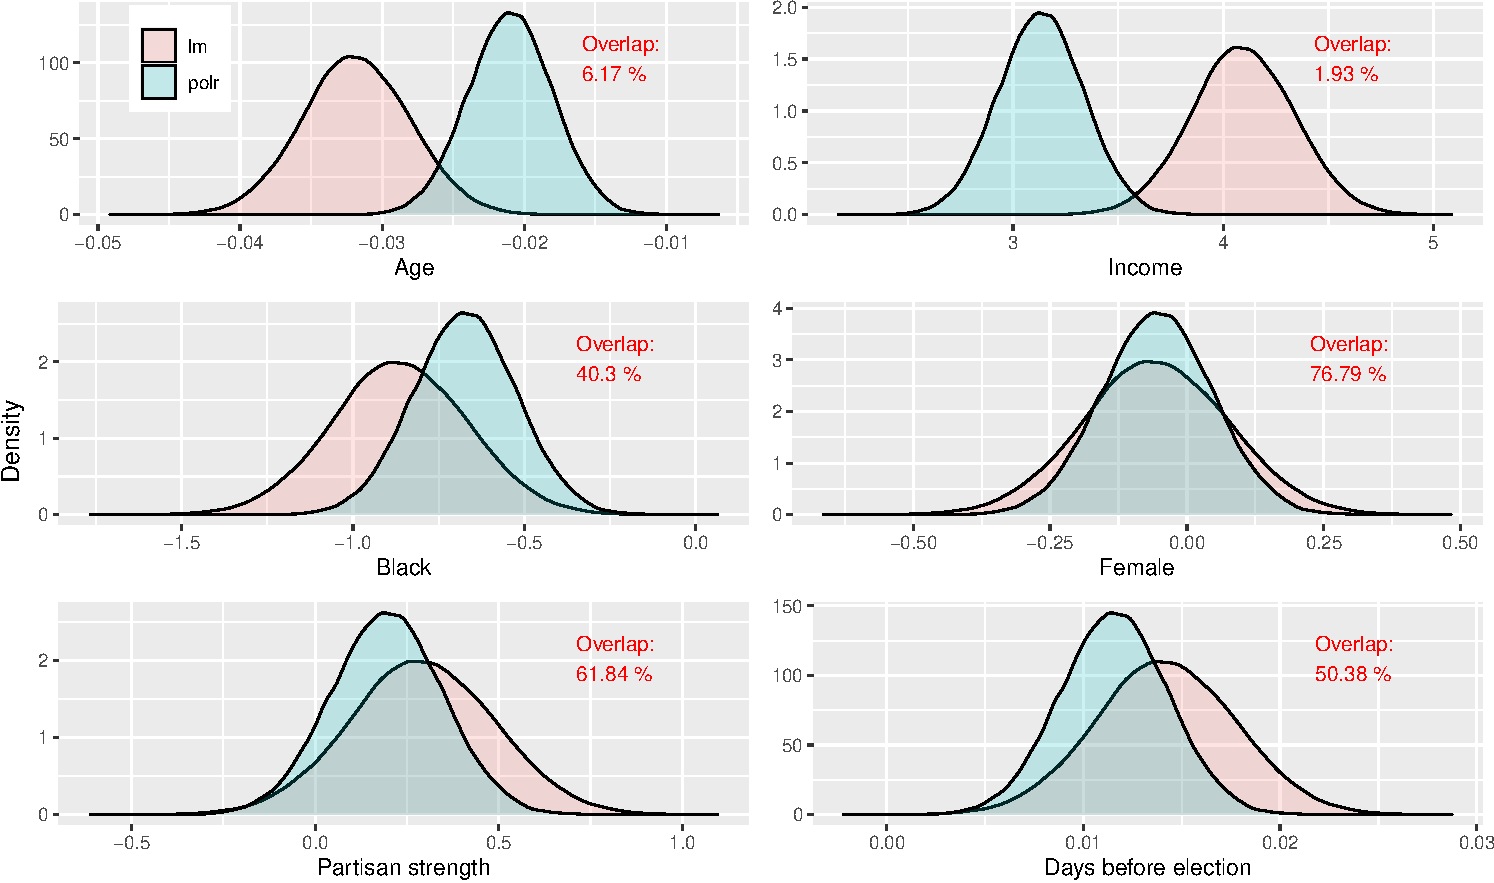
\includegraphics{dissertation_files/figure-latex/Density-Plots-Bartels-1992-1.pdf}
\caption{\label{fig:Density-Plots-Bartels-1992}Distributions of \texttt{lm} and \texttt{polr} Coefficients in 1992 ANES Data as Used by Bartels (1999)\label{DensBart92}}
\end{figure}
We observe a small posterior percentage of overlay for the distributions of \texttt{Age} and \texttt{Income} (\textless{} 10 percent) and a large posterior percentage of overlay for the distributions of \texttt{Black}, \texttt{Female}, \texttt{Partisan\ strength}, and \texttt{Days\ before\ election} (\textgreater{} 40 percent). Since a large percentage indicates little difference in significance between the two sets of coefficients, these results appear provide evidence against the importance of re-estimating ordinal variable categories with an ordered probit model. It seems that uneven distances between ordinal variable categories might not actually be of crucial importance when it comes to missing data imputation.

\hypertarget{ordmiss-conclusion}{%
\section{Conclusion}\label{ordmiss-conclusion}}

I set out to improve multiple imputation results with ordinal variables by accounting for the unevenly spaced ordering contained in ordinal variables. I did so by adapting the multiple hot deck imputation function \texttt{hot.deck} to treat ordinal variables with an ordered probit model in order to estimate numerical thresholds from an assumed underlying latent continuous variable. The results clearly show diverging outcomes from the different algorithms, with each algorithm behaving differently under changing circumstances.

\texttt{hd.ord} performs on par with some binary variables but overall worse than \texttt{amelia} and \texttt{mice} for data MAR with 5 variables with missing values. The results for the MNAR analyses paint a more mixed but overall unchanged picture. \texttt{hd.ord} performs somewhat better for binary variables but remains the least accurate method for interval and ordinal variables. Increasing the number of ordinal variables included in the \texttt{polr} treatment does not have a positive effect on the performance of \texttt{hd.ord}. In fact, \texttt{hd.ord} consistently performs slightly worse for both data sets for all mechanisms of missingness. Unlike \texttt{amelia} and \texttt{mice}, \texttt{hd.ord}'s performance also drastically worsens when the percentage of missingness in the data is increased to 50 percent.

On the positive side, \texttt{hd.ord} performs multiple imputation much more quickly: \texttt{amelia} and \texttt{mice} are at least 3.8 and 20.6 times slower than \texttt{hd.ord} for 20 percent of missing data, respectively. This speed gain is of dubious value, however. While it is necessary to iterate multiple imputation runs many times over for simulation purposes like this one, users likely will not do so, which greatly diminishes the computing time saved. Even if users do opt to run multiple imputation for 1,000 times, the differences in terms of absolute time for \texttt{amelia} are not so great as to be impractical. \texttt{amelia} took at most a little under 11 minutes to compute 1,000 iterations of multiple imputation for 20 percent missing data, regardless of the data set in question. In absolute terms, this is not a lot of time for the general user to invest in data preparation. With a minimum of just over 50 minutes, the same cannot be said for \texttt{mice}. Nonetheless, \texttt{hd.ord}'s speed gain over \texttt{amelia} cannot be considered enough reason to choose \texttt{hd.ord} over \texttt{amelia}, unless the data consists of exclusively binary variables where the differences between \texttt{hd.ord} and \texttt{amelia} are small.

Given all the above, the result of this quality comparison of major missing data solutions is a clear endorsement of \texttt{amelia}. It performs well for all types of variables in all stages of missingness and does so in a reasonably short amount of time. The combination of EM with bootstrapping clearly represents a great improvement in terms of speed over IP used in \texttt{mice}. While it offers a wealth of sophisticated options for specialized users, \texttt{amelia}'s default out-of-the-box settings are simple and intuitive for general users. On top of that, it is notable that \texttt{amelia} produces better results than \texttt{na.omit} when data is MNAR, i.e.~it performs well in a setting it was not designed for. \texttt{amelia} thus represents the best \texttt{R} solution to problems of missing data for general users.

While \texttt{hd.ord} did not yield the desired improvements, my analysis provides in-depth insights into and corroborates the robustness of multiple imputation implementations like \texttt{amelia} and \texttt{mice} for a variety of variable types in survey settings.

\hypertarget{framing}{%
\chapter{MORALITY, SELF-INTEREST, AND FRAME STRENGTH}\label{framing}}

\hypertarget{framing-intro}{%
\section{Introduction}\label{framing-intro}}

In today's world, we rarely consume information directly, for instance by attending a demonstration or listening to a talk. Instead, most of the information we consume is mediated through television, radio, blogs, social media, messenger apps, and so forth. Mediated information by definition only represents a selective fragment of reality. The messenger -- news anchors, pundits, influencers, politicians etc. -- makes conscious and unconscious choices what information to distribute and how to present this information to us. The mediated message that eventually reaches us has been manipulated, often not intentionally. Numerous strategies to carry out such manipulations exist. One of these strategies is framing.

Framing is the practice of presenting an issue to affect the way people see it (Chong \& Druckman, 2007). It reorganizes existing information already present in people's minds and attempts to direct people's attention towards particular considerations (Druckman \& Nelson, 2003). Numerous experiments have shown that frames can have substantial influence on people's opinions (Chong \& Druckman, 2010; Sniderman \& Theriault, 2004). Work remains, however, to uncover which types of frames have more influence than others. I provide an avenue of clarification by testing the influence of morality and self-interest in political framing.

For some time, scholars have postulated the `death' of self-interest to explain issue positioning: People eschew their self-interest to defend and vote according to their morals instead, as they consider them more important (Frank, 2004; Haidt, 2008). Others, however, cast doubt on these claims: Morality and cultural values do not outweigh self-interest concerns, which in turn represent a significant factor in determining issue positioning (Bartels, 2005, 2006). Which is it? Have moral concerns displaced self-interest? Does self-interest matter more than postulated by many? I intend to shed some light on these questions with an online framing survey experiment that directly juxtaposes morality and self-interest. Morality is assessed on the basis of Moral Foundations Theory (Haidt, 2012). Self-interest is defined to include any goals related to personal autonomy, health/safety, wealth, and status (Gintis, 2017; Weeden \& Kurzban, 2017). Demographic information and conviction measurements are used to analyze the influence of each concept. To my knowledge, this setup has not been studied before. In addition to the substantive analysis, both methods developed in chapters \ref{ordblock} and \ref{ordmiss} are applied and their performance is analyzed.

\hypertarget{framing-theory}{%
\section{Theory}\label{framing-theory}}

\hypertarget{framing-theory-framing}{%
\subsection{Framing}\label{framing-theory-framing}}

People usually do not have stable, consistent, and informed opinions (Converse, 1964; Zaller, 1992). It is possible to influence people's opinion through communication. One of the ways to do so is framing, which is the practice of presenting an issue to affect the way people see it (Aaroe, 2011; Druckman, 2001a; Gross, 2008). We learn about issues such as healthcare reform through articles, reports, speeches, commercials and social media. This mediated communication possesses tremendous potential influence on our perception of political issues (Iyengar, 1996; Kam \& Simas, 2010; Tversky \& Kahneman, 1981). Framing research has established that a variety of frames substantively influence how people view and think about issues (Andsager, 2000; Callaghan \& Schnell, 2005; Entman, 1993, 2004; Gamson \& Modigliani, 1989; Lahav \& Courtemanche, 2012; Pan \& Kosicki, 1993; Price, Tewksbury, \& Powers, 1997; Slothuus \& Vreese, 2010; Sniderman \& Theriault, 2004; Vreese, 2004). When frames influence people's opinion about an issue, we speak of a framing effect. Two different types of framing effects have evolved in the literature: equivalency and emphasis framing effects.

\hypertarget{framing-theory-framing-equiv}{%
\subsubsection{Equivalency Framing}\label{framing-theory-framing-equiv}}

Equivalency framing involves phrasing the same logical content in different ways, i.e.~``casting the same information in either a positive or negative light'' (Druckman, 2004, p. 671). One example is Tversky \& Kahneman (1981)'s death and survival experiment (see page \pageref{death}): Presented with a hypothetical disease outbreak in the US that is expected to kill 600 people, respondents are asked to choose between alternating programs. The first group chooses between programs A and B. In program A, ``200 people will be saved''. In program B, ``there is a 1/3 probability that 600 people will be saved and a 2/3 probability that no people will be saved''. The second group chooses between programs C and D. In program C, ``400 people will die''. In program D, ``there is a 1/3 probability that nobody will die, and a 2/3 probability that 600 people will die''. The factual content given to both groups is of identical: In both groups, the first program results in the death of 400 people and the second program has a 66 percent chance of killing all 600 people. The difference is the light cast on this information. The frames given to group 1 focus on lives saved, whereas the frames presented to group 2 center around lives lost. Rationally, both are the same. However, this difference in equivalency framing matters: When the experiment was run, the majority in group 1 chose program A. The majority in group 2 chose program D. Framing thus greatly shifted support for the programs.

Other scholarly framing work focuses on policy evaluations, rather than risk preferences. For example, respondents are found to rate a proposed economic program more favorably when it is framed as resulting in 95 percent employment, instead of its logical equivalent of 5 percent unemployment (Quattrone \& Tversky, 1988). Equivalency framing effects have been likened by some to survey question wording effects (Zaller, 1992). Examples here are the alternate use of ``not allow'' and ``forbid'' in reference to Communist speech in the 1970s, which can arguably be described as substantively and logically equivalent (Bartels, 2003, p. 61).

\hypertarget{framing-theory-framing-emph}{%
\subsubsection{Emphasis Framing}\label{framing-theory-framing-emph}}

Emphasis framing on the other hand stresses a particular aspect, viewpoint, or consideration about an issue in the attempt to get people to look at the issue in the proposed way. Describing the invasion of Iraq as freeing the population and gifting them democracy, as done by the Bush administration, for instance, emphasizes a very different viewpoint than a possible alternative narrative that focuses on the economic benefits of gaining access to oil fields and trade opportunities. Unlike equivalency frames, emphasis frames are not logically identical ways of phrasing the same issue. Instead, they highlight qualitatively different considerations of that issue (Druckman, 2001c, 2001b; Kinder \& Sanders, 1996; Levin, Schneider, \& Gaeth, 1998; Nelson \& Kinder, 1996; Sniderman \& Theriault, 2004), forcing people to think about the importance of the considerations suggested by the frame (Nelson, Clawson, \& Oxley, 1997).

My focus lies on emphasis frames. An abundance of experiments have shown that emphasis frames elicit significant changes in issue positioning (Chong \& Druckman, 2010, 2013; Druckman, 2001b; Druckman, Fein, \& Leeper, 2012; Druckman \& Nelson, 2003; Druckman et al., 2013; Nelson et al., 1997; Slothuus, 2008). Brewer \& Gross (2005), for instance, find significant effects for the frames ``School vouchers create an unfair advantage'' and ``School vouchers provide help for those who need it''. Druckman et al. (2012) provide similar evidence for ``The Affordable Care Act gives more people equal access to health insurance'' and ``The ACA increases government costs'', while Druckman et al. (2013) do so for ``Oil drilling provides economic benefits'' and ``Oil drilling endangers marine life''. Despite the mass of experimental framing research, however, we still have little insight into what makes an emphasis frame strong. We don't know why some emphasis frames elicit effects and others don't, i.e.~we don't know why some frames are strong and other frames are weak. Chong \& Druckman (2007) attempt a differentiation into weak and strong frames. They ask respondents in a pre-test what arguments the respondents consider strong or weak for a variety of chosen issues. Frames containing strong arguments are then deemed strong frames, while frames containing weak arguments are considered weak frames. These weak and strong frames are then used in the subsequent framing experiment. While it is no doubt laudable to explore which arguments in selected political issues are deemed more persuasive than others, this setup does not provide insights as to what actually makes a frame strong or weak. We simply know which arguments (to then be embedded in frames) are considered to be strong and weak, but not why. A major challenge for framing research thus still ``concerns the identification of factors that make a frame strong'' (Chong \& Druckman, 2007, p. 116).

In the attempt to address this challenge, scholars have increasingly adopted theory-driven approaches that deduce likely strong frames and subsequently empirically evaluate their theoretical expectations. Arceneaux (2012) for instance theorizes that ``individuals are more likely to be persuaded by political arguments that evoke cognitive biases'' (p.~280) and asserts that messages which highlight out-group threats resonate with respondents to a greater extent. Druckman \& Bolsen (2011) report that adding factual information to messages about carbon nanotubes does nothing to enhance their strength and actually makes the message weaker. Feinberg \& Willer (2013) assess whether frames are stronger when they cohere with an individual's personal value system. They frame environmental issues as a matter of moral `purity', a theme that supposedly correlates with conservative ideology, and find this approach leads to increased conservative support of environmental policies. I attempt to provide a further avenue of clarification by investigating how morality and self-interest contribute to persuasive strength in emphasis framing.

\hypertarget{framing-theory-morality}{%
\subsection{Morality}\label{framing-theory-morality}}

Two of the main ingredients of public opinion are commitment to moral principles and interests that citizens see at stake (Kinder, 1998). Morality plays a role in establishing one's self-concept and identity. Moral arguments are ubiquitous in political issues because they are essential to how people perceive and make sense of the world around them (Cervone, 2004; Frank, 2004; Mooney, 2001; Skitka, Bauman, \& Mullen, 2008; Tatalovich, Smith, \& Bobic, 1994). They present themselves in the form of `oughts' and `shoulds' (Rokeach, 1968). People feel that moral arguments (1) represent near-universal standards of truth, (2) are almost objective facts about the world, and (3) exist independent of institutional authority (Skitka, 2010). It is widely argued that people rely to a disproportionate extent on moral arguments to form their opinions since moral arguments achieve a high emotional connection due to invoked values and feelings (Bauman \& Skitka, 2009; Haidt, 2003b; Ryan, 2014a, 2014b; Skitka, Bauman, \& Sargis, 2005; Skitka \& Wisneski, 2011; Smith, 2002; Tatalovich \& Daynes, 2011). Emotions play an important role in how people conceptualize moral stimuli since people feel emotionally committed to their values (Feinberg \& Willer, 2013; Ryan, 2014b; Suhay, 2008; Tetlock, Peterson, \& Lerner, 1996).

\hypertarget{framing-theory-morality-issues}{%
\subsubsection{Moral vs.~Non-Moral Issues}\label{framing-theory-morality-issues}}

A lot of scholarly work tries to establish a distinction between moral and non-moral issues, yet agreement on the definition of a `moral issue' remains elusive. To some, an issue is moral when at least one side sees the issue as threatening a core value/principle and/or uses moral arguments to support their position (Haider-Markel \& Meier, 1996; Mooney, 2001). To others, moral issues are based on values rooted deeply within people's belief systems (Biggers, 2011; Glick \& Hutchinson, 2001). Yet another strain sees morality as intrinsic to some issues, i.e.~non-technical issues that are easy to understand or issues that concern fundamental aspects of life and death (Studlar, 2001; Tavits, 2007). Yet others again assert that economic issues are not to be considered moral (Abramowitz, 1995; Engeli, Green-Pedersen, \& Larsen, 2012; Mooney \& Lee, 1995; Tatalovich \& Daynes, 2011) despite evidence to the contrary: Ryan (2014b) finds that some people perceive distinctly economic issues such as labor relations or social security reform in moral ways. In addition, studies on abortion show that, despite widespread media depiction to the contrary, not everyone conceives of it as a moral issue (Mullen \& Skitka, 2006; Skitka, 2002; Skitka et al., 2005). Assertions of moral and non-moral issues are misleading and unnecessary. Instead, we should concern ourselves with the moral and non-moral content of each respective issue. I thus eschew moral and non-moral issue definitions and focus on moral and self-interest frames within issues, rather than the moral nature of the issues themselves.

\hypertarget{framing-theory-morality-mft}{%
\subsubsection{Moral Foundations Theory}\label{framing-theory-morality-mft}}

In normative terms, we differentiate between prescriptive and proscriptive morality, which are based on approach-avoidance differences in self-regulation (Carnes \& Janoff-Bulman, 2012). Prescriptive morality is sensitive to positive outcomes and focused on what we should do. Proscriptive morality is sensitive to negative outcomes and focused on what we should not do (Janoff-Bulman et al., 2009). Based on this categorization, Haidt and his colleagues developed Moral Foundations Theory (MFT), which encompasses cognitive foundations of moral matrices and has become widely adopted in moralization literature (Clifford et al., 2015a; Clifford \& Jerit, 2013; Feinberg \& Willer, 2013; Graham, Haidt, \& Nosek, 2009; Haidt, 2001, 2003a, 2003b, 2007, 2008, 2012; Haidt \& Graham, 2007; Haidt \& Joseph, 2004, 2007; Haidt \& Kesebir, 2010; Hofmann, Wisneski, Brandt, \& Skitka, 2014; Koleva, Graham, Iyer, Ditto, \& Haidt, 2012; Schein \& Gray, 2017). These foundations are shown in Table \ref{framing-foundations}.
\begin{table}[!htbp]
\caption{Foundations of Moral Intuitions}
\centering
\resizebox{\textwidth}{!}{
\begin{tabular}{>{\itshape}l ll >{\itshape}l l}
\bottomrule 
\midrule
\multicolumn{2}{c}{\textbf{Positive}} & & \multicolumn{2}{c}{\textbf{Negative}}\\
\cmidrule{1-2}
\cmidrule{4-5}
Care & Cherishing, protecting others & & Harm & Hurting others\\
Fairness & Rendering justice by shared rules & & Cheating & Flouting justice/shared rules\\
Loyalty & Standing with your group & & Betrayal & Opposing your group\\
Authority & Submitting to tradition/authority & & Subversion & Resisting tradition/authority\\
Sanctity & Repulsion at disgust & & Degradation & Enjoyment of disgust \\
Liberty & Acting without constraint & & Oppression & Dominate/Constrain others\\
\bottomrule
\multicolumn{5}{l}{\footnotesize{Positive and negative foundations are conceptual opposites.}} \\
\end{tabular}}
\label{framing-foundations}
\end{table}
Moral intuitions are a powerful psychological mechanism that underlies issue positions (Koleva et al., 2012). Haidt and his colleagues argue that they intuitions are rooted in evolved mechanisms. They propose that Care/Harm developed as the response to the adaptive challenge of protecting and caring for children. It makes us sensitive to signs of suffering and activates us to care for those who are being harmed. Fairness/Cheating developed as the response to acts of cooperation or selfishness that people show towards us. It makes us trust fair actors and punish cheaters. Loyalty/Betrayal developed to meet the adaptive challenge of forming and maintaining cohesive coalitions. It makes us reward loyalty and ostracize those who betray us. Authority/Subversion developed as the response to forging beneficial relationships within social hierarchies. It makes us sensitive to signs that people do not behave in accordance with their social position. Sanctity/Degradation developed as a response to the challenge of living in a world full of pathogens and parasites. It binds us into moral communities by shared notions of sacredness. Liberty/Oppression developed as a response to the challenge of living in small groups whose members can dominate and constrain us. It makes us value freedom and reject repression.

Because of the deep connection between morality and emotions, people have a tendency to internalize and defend their values. This ``makes it very difficult for people to consider the possibility that there might really be more than one form of moral truth, or more than one valid framework for judging people or running a society'' (Haidt, 2012, p. 111). Haidt distinguishes the use of these foundations by ideology. According to him, liberals tend to utilize a three-foundation morality, whereas conservatives allegedly lean towards using all six foundations. He also estimated the means of each moral foundation on a 6-point Likert scale (``Not at all relevant'' to ``Extremely relevant''). Liberals score 3.62 in Harm and 3.74 in Fairness but only 2.07 in Loyalty, 2.06 in Authority, and 1.27 in Sanctity. Conservatives score 2.98 in Harm, 3.02 in Fairness, 3.08 in Loyalty, 3.28 in Authority, and 2.89 in Sanctity (Graham et al., 2011). Additionally, both sides tend to focus on different aspects in the three foundations they share (Care/Harm, Fairness/Cheating, Liberty/Oppression): Conservatives are more likely to emphasize society's protection and security and aim to prevent losses and generally negative outcomes, while liberals tend to emphasize the provision of welfare for others and aim to advance gains and generally positive outcomes. Both are said to seek normatively `good' outcomes for society, but with different orientations (Janoff-Bulman, 2009; Janoff-Bulman \& Carnes, 2013; Janoff-Bulman et al., 2009).

While the liberal/conservative divide of course plays a role in opinion formation, it is not central to moral analyses. Liberals and conservatives are said to display differing tendencies towards each individual foundation, but the majority of people value all foundations. The foundations themselves, not party ID, are what matters most. I thus use the foundations as the building block of moral arguments in my juxtaposition of morality and self-interest.

\hypertarget{framing-theory-self_interest}{%
\subsection{Self-Interest}\label{framing-theory-self_interest}}

Self-interest refers to actions or behaviors that elicit personal benefit. When acting in self-interest, individuals look out for themselves and act on the grounds of personal gains (Arrow, 1967; Coleman, 1986; Downs, 1957; Ferejohn \& Fiorina, 1974; Fiorina, 1977; Olson, 1965; Riker \& Ordeshook, 1968; Sears \& Funk, 1991). In neoclassical economics, this claim is extended to the overall postulation of human beings as \textit{homines economici} (Coleman, 1986); creatures who act strictly rationally with the intent to maximize utility at all times. In political psychology, scholars instead focus on the importance of self-interest as a motivation for opinions on political issues.

In the 1960s, self-interest was considered a major determinant of opinions on political issues. Campbell, Converse, Miller, \& Stokes (1960) for instance report that people with less income and education are more likely to support a strong government role in the provision of social welfare, stating that ``people presented with certain policy alternatives can do a reasonable job of selecting responses that appear to further their self-interest'' (p.~208). Empirical research from the 1970s and 1980s appears to confirm this (Batson, 1991; Etzioni, 1988; Feldman, 1982, 1984; Friedland \& Robertson, 1989; Hirschman, 1985; Kohn, 1990; Lau \& Sears, 1981; Lerner, 1980; Mansbridge, 1990b; Miller \& Ratner, 1996; Schwartz, 1986; Sears \& Citrin, 1985; Weatherford, 1983). Hawthorne \& Jackson (1987) find that income level and tax bracket significantly predict support for the tax cuts in the 1978 federal Tax Revenue Act. Lau, Coulam, \& Sears (1983) identify a similar relationship for high taxpayers in their Massachusetts income tax study. Coughlin (1990) discover that higher income citizens oppose redistribution slightly more than those with lower income. Sears, Lau, Tyler, \& Allen (1980) and Sears \& Lau (1983) find evidence for pocketbook voting in their studies on government-guaranteed full employment. Courant, Gramlich, \& Rubinfeld (1980) discover modest but consistent effects for the perceived property tax burden in Michigan. Lau, Sears, \& Jessor (1990) find a significant relationship between perceived financial situation and anti-incumbent voting. The analysis by Sears \& Lau (1983) reveals that perceived personal federal tax burden predicts support for the tax cuts specified in the 1979 Kemp-Roth bill. Bartels (2005) identifies a high subjective tax burden as the source of support for the 2001 and 2003 Bush tax cuts. Sears \& Citrin (1985) similarly find that citizens with a high subjective tax burden acted out of self-interest in the so-called California Tax Revolt at the end of the 1970s.

Despite this evidence, an abundance of criticism has claimed the inadequacy of self-interest as a major predictor of human behavior. Miller \& Ratner (1996) call ``homo economicus (\ldots) a social construction, not a biological entity'' (p.~45). Human behavior is argued to be too complex and much more than self-interest is claimed to come into play when people think about what they want in life (Batson, 1991; Friedland \& Robertson, 1989; Kohn, 1990; Lerner, 1980; Mansbridge, 1990b, 1990a; Schwartz, 1986; Sen, 1977; Tyler, 1990b). The study of social movements, for instance, asserts clear evidence that motivations other than self-interest also majorly account for human behavior (Mansbridge, 1990c). The overall most important reasons for humans' choices are said to be affective and normative (Etzioni, 1988) and researchers are urged to shift their focus away from the obsession with self-interest and towards moral values (Hirschman, 1985). The dominant theories of motivation are said to be fundamentally based on personal gains and miss the influence that values and ideologies have on people's attitudes towards policies (Sears \& Funk, 1990). People are asserted as more interested in the fairness of procedures and policies than the self-beneficial outcomes of these processes (Brockner, 2002; Hollander-Blumoff \& Tyler, 2008; Tyler, 1990a). When procedural fairness is high or perceived as being high, it is argued that outcome favorability is likely to decline as participants consider themselves heard and listened to (Gibson, 2002; Tyler \& Caine, 1981; Vidmar, 1990).

Others critique that it is possible and plausible for self-interest to play a role in opinion formation, but even then it does not play the only role (Chong, Citrin, \& Conley, 2001; Citrin \& Green, 1990; Miller, 1999; Sears \& Funk, 1990). It is argued that self-interest is limited in explanatory scope (Chong et al., 2001; Huddy, 2013; Kinder, 1998; Lau \& Heldman, 2009; Lewis-Beck, Jacoby, Norpoth, \& Weisberg, 2008; Sears \& Funk, 1990) and only applies to short-term material gains (Sears et al., 1980). As a result, self-interest is seen as negligible: ``Many political scientists used to assume that people vote selfishly, choosing the candidate or policy that will benefit them the most. But decades of research on public opinion have led to the conclusion that self-interest is a weak predictor of policy preferences'' (Haidt, 2012, p. 85). Furthermore, standard demographic measures such as education, income, race, and gender are not deemed adequate indicators of self-interest, thus discounting findings from the 1960s (Kinder, 1998; Sears \& Funk, 1990).

Countering such criticism, a different group of scholars assert that self-interest does indeed form a major predictor of human behavior. They argue that the self-interest criticism defines away any chance of self-interest being a major determinant of political opinion by restricting it to financial benefits and declaring ordinary demographic effects uninterpretable: Instead of a restricted categorization as purely economic gains, self-interest can be defined as ``advancing any of a range of people's typical goals, whether directly involving material gain or not, whether involving immediate gain or something more subtle that advances someone's progress over the longer term'' (Weeden \& Kurzban, 2014, p. 38). Following evolutionary psychology, self-interest thus applies not only to economic aspects and material gains but also to various social and cultural domains (Buss, 2015; Kurzban et al., 2010; Nteta, 2013; Petersen, 2016). This includes emotions, which are evoked whenever a person's self-interest goals are advanced or threatened (Lazarus, 1994). Self-serving preferences range from having more money to gaining prestige, having sex, or wishing success for one's children, among many others (Becker, 1996; Owens \& Pedulla, 2014; Weeden, 2015; Weeden \& Kurzban, 2016). Self-interest is here defined as related to personal autonomy, health/safety, wealth, and status (Gintis, 2017).

Defining self-interest in exclusively material terms seems needlessly restrictive, as is concluding that self-interest is not a valid predictor of human behavior. For one, empirical evidence indicates that self-interest at least plays some role for economic aspects. For another, arguing that self-interest does not matter because of its exclusive focus on material gains after having defined self-interest in precisely this way has the feel of a snake biting its own tail. Self-interest is unlikely to matter for many policy preferences when it is restricted to purely economic matters, but such a narrow definition appears unwarranted. Material gains are not all that humans desire. It is much more plausible that self-interest covers a range of people's self-advancing goals instead. As a result, I follow the definition of self-interest as one of personal autonomy, health/safety, wealth, and status.

\hypertarget{framing-design}{%
\section{Design}\label{framing-design}}

Each of the previous areas has been studied, but they have not been applied together. An abundance of framing research exists and we know that emphasis frames can be successful in directing people's attention towards particular considerations of an issue, but we still don't know why some emphasis frames succeed while others fail. We know that morality plays a large role in people's issue positioning and that self-interest accounts for some human behavior, but we don't know how much self-interest and morality matter in direct comparison when people choose issue positions. I conduct a framing experiment that explores what we don't know by investigating how morality and self-interest contribute to persuasive strength in emphasis framing.

Juxtaposing morality and self-interest in frames follows the recognition that people don't just want to satisfy their interests, but neither do they completely set aside their self-regarding preferences in favor of altruistic motives (Stoker, 1992). Both concepts are in constant movement, depending on the situation. People deal with the `central problem of ethics': ``how the lives, interests, and welfare of others make claims on us, and how these claims, of various forms, are to be reconciled with the aim of living our own lives'' (Nagel, 1970, p. 142). Support for issues, for instance the welfare state, is based on ``generalized and reciprocal self-interest'' (Baldwin, 1990, p. 299), i.e.~it depends on both value-based attitudes and immediate self-interest (for macro factors influencing welfare support, such as a country's social structure and major institutions, see Brooks \& Manza, 2007).

Opinions can be influenced by self-interest or alterations in empathy towards others (Hacker, Rehm, \& Schlesinger, 2013; Rehm, Hacker, \& Schlesinger, 2012). It is often difficult to tell which is which: Frank (2004) claims Republicans have duped rural and working-class Americans into voting against their self-interest by supporting Republican tax cuts that negatively affect them financially. Bartels (2005) however argues that they instead vote in unenlightened self-interest because they perceive their personal tax burden to be too high and (falsely) believe tax cuts can lower them. Haidt (2012), finally, states that they vote for their moral interest, as they don't want the country to devote itself primarily to the pursuit of social justice. It is difficult to assess which is correct.

Previous studies and experiments on moral framing that utilize MFT focus on partisan division (Clifford \& Jerit, 2013; Feinberg \& Willer, 2013; Koleva et al., 2012; Slothuus \& Vreese, 2010; Wolsko, Ariceage, \& Seiden, 2016). Party ID is not central to analyses of moral concerns, though it undoubtedly matters in political analysis. I thus do not focus on party ID but instead utilize MFT to focus on the morality vs.~self-interest juxtaposition within framing whilst also accounting for the influence of party ID as a possible moderator. I combine emphasis framing with aspects of MFT and the literature on self-interest.

\hypertarget{framing-design-issues-frames}{%
\subsection{Issues and Frames}\label{framing-design-issues-frames}}

Issues are selected from previous research and based on suitability to assess self-interest and morality. In order to assess self-interest, all issues need to apply directly to respondents' daily lives (DeScioli, Cho, Bokemper, \& Delton, 2020; Kurzban, 2010; Sznycer et al., 2017). I design frames that propose new policies in the areas of healthcare and the environment. Everyone is affected by healthcare in their lives, so everyone has a vested self-interest in this issue. At the same time, how much the government should be involved in the provision of healthcare coverage is the subject of great debate. Similarly, everyone is affected by the environment, resulting in viable cause for self-interest, while the topic is also highly controversial in moral terms.

Each respondent is presented with one of five randomly assigned frames for each issue: an issue-supporting moral frame, an issue-opposing moral frame, an issue-supporting self-interest frame, an issue-opposing self-interest frame, or the control frame. The design consists of issue-supporting and issue-opposing frames in order to control for both signs in determining frame strength. The self-interest frames aim to activate each respondent's self-interest as identified by Weeden \& Kurzban (2014). The moral frames are designed on the basis of MFT. For simplicity and to avoid cluttering, I only use the foundation that most applies to each issue and to the majority of people. For both issues, that is Care/Harm. Support/Opposition for/to the frame's content is assessed on a 5-point Likert scale (Q27 (healthcare) and Q30 (environment) in the questionnaire).\footnote{The complete questionnaire in chronological order with all frames can be found in appendix section \ref{framing-questionnaire}.} The self-interest frames are based on prior research (Gerbasi \& Prentice, 2013).

Each issue frame consists of an identical paragraph of information and a paragraph containing the morality/self-interest content. The frames for healthcare introduce a potential new healthcare plan that covers everyone in the US, is paid for with a mix of fees paid by individuals and employers as well as tax dollars, and provides free healthcare for all services and drugs to those over 65 and those with low income. The frames for the environment introduce potential new environmental regulations which restrict the use of toxic pesticides that might contaminate crops, soil, and ground water and that are particularly harmful to the elderly and those with various medical conditions. The environmental information paragraph also states that farmers receive state subsidies to cover parts of their increased costs as a result of these restrictions. The control frames contain just the introductory paragraph of information without any added content.

Prior to frame treatment, respondents answer a series of questions to measure their morality and self-interest levels. To measure morality, respondents are asked to identify the personal relevance of six questions on emotional suffering, caring for the vulnerable, cruelty, compassion, hurting animals, and killing human beings (Q4-Q9). These questions are taken from the Moral Foundations Questionnaire (Haidt, 2012). To measure self-interest, respondents similarly state the personal relevance of six statements about telling white lies, caring for friends and family over others, giving your own children advantages over others, choosing to kill over being killed, lying for your own good, and helping those who help you (Q10-Q15). These questions are taken from Raine \& Uh (2019). The questionnaire also collects standard demographic information (Q16-Q18, Q20-Q26) and gives respondents the chance to enter comments (Q33). The question inquiring after respondents' education (Q26) is split into two sets (ANES, ordered probit) of education categories to allow for a comparison of results. The survey starts with questions about respondents' online work as a means to ease entry into the survey (Q1-Q3).

\hypertarget{framing-design-checks}{%
\subsection{Attention and Manipulation Checks}\label{framing-design-checks}}

The questionnaire contains an attention check (Q19) which is used to filter out inattentive respondents as they answer the survey. The check asks respondents to identify the correct statement (``The letter B comes before the letter K in the alphabet'') amongst a list of three false statements. If respondents fail to give the correct response, the website terminates the survey and their data is not processed. Respondents are not allowed to continue the survey and drop out of the sample. This happens after the morality and self-interest questions as part of the demographics and is treatment-independent. Respondents who fail the check drop out of the survey before they are assigned to treatment groups. Attention checks, or instructional manipulation checks, are commonly used to avoid respondent satisficing, i.e.~selecting responses without paying attention to the instructions (Anduiza \& Galais, 2016; Clifford \& Jerit, 2014; Curran, 2016; Krosnick, Sowmya, \& Smith, 1996; Oppenheimer, Meyvis, \& Davidenko, 2009). The idea is to filter out inattentive respondents who provide low-quality data.

The questionnaire also contains factual manipulation checks after each frame (Q29 and Q32). These checks inquire after the nature of the political topic just discussed. Respondents are asked to identify the correct issue (healthcare, environment) out of a list of seven political topics. Unlike the attention check, the factual manipulation checks do not determine whether respondents can continue the survey. All respondents who are presented with treatment frames remain part of the sample, regardless of their answers to the factual manipulation checks. The checks are not used to filter out respondents. Doing so could introduce post-treatment bias of causal effects (Montgomery, Nyhan, \& Torres, 2018). In any randomized experiment, the ability to establish causality rests on the comparison of similar pre-treatment groups that act as each other's counterfactuals (Berinsky, Margolis, \& Sances, 2014; Horiuchi, Imai, \& Taniguchi, 2007). Conditioning on a post-treatment manipulation check invalidates this comparison because we are then comparing two dissimilar groups. Conditioning on these variables can lead to sample imbalance regarding observed and unobserved confounders. Respondents who fail the check in one treatment group might not look like respondents who fail the check in a different group (Acharya, Blackwell, \& Sen, 2016; Aronow, Baron, \& Pinson, 2019; Healy \& Lenz, 2014). Instead, these checks are solely used in post-experiment analysis to estimate any potential differences between attentive and less attentive respondents in terms of issue support (Kane \& Barabas, 2019). All question wordings are based the ANES, CCES, and GSS surveys.\footnote{In line with modern social science transparency (Ioannidis, 2005; Miguel et al., 2014), the experimental design, the hypothesis, and the planned regression models were pre-registered with the Open Science Foundation prior to data analysis: \url{https://osf.io/tvpwq/}}

\hypertarget{framing-design-expectations}{%
\subsection{Expectations}\label{framing-design-expectations}}

Moral arguments are said to relate more strongly than non-moral ones since they are deeply connected to emotions. Non-moral arguments, on the other hand, are said to be more loosely connected to emotions and thus deemed less powerful (Haugtvedt \& Wegener, 1994; Johnson \& Eagly, 1989). This would suggest that moral frames exert a stronger influence on respondents' issue positioning than self-interest frames. The effect of different frames should also be differently felt conditional on respondents' own moral and self-interest priorities. A moral frame should affect respondents' opinion more if they score highly on the moral measures as this type of frame is likely to connect more with their values. Likewise, a self-interest frame should register more strongly with respondents if they score highly on the self-interest measures. I thus post the following hypotheses:

\vspace{0.3cm}
\begin{adjustwidth*}{+1cm}{+1cm}
\noindent \textbf{H1.} Moral frames move people more than self-interest frames.\\
\noindent \textbf{H2.} Moral frames move people with higher morality scores more than people with lower morality scores.\\
\noindent \textbf{H3.} Self-interest frames move people with higher self-interest scores more than people with lower self-interest scores.\\
\end{adjustwidth*}
\hypertarget{framing-data}{%
\section{Data}\label{framing-data}}

\hypertarget{framing-data-mturk}{%
\subsection{MTurk}\label{framing-data-mturk}}

The data consist of a randomized survey experiment and an accompanying pre-test, both fielded online. Pre-testing frames with participants who are not part of the main survey experiment is crucial in framing analysis to test the mechanisms of the designed questionnaire (Carpini \& Keeter, 1993; Conover, Crewe, \& Searing, 1991; Stanley, 2016). The participants are exposed to the designed frames to test the core ideas behind morality and self-interest. This pre-test structure builds on work by Slothuus \& Vreese (2010), Chong \& Druckman (2007) and the mass communication and persuasion literature (O'Keefe, 2002). The pre-test is carried out on Amazon's online platform MTurk.

MTurk is a service where researchers can host tasks to be completed by anonymous participants. Participants receive financial compensation for their work and Amazon collects a commission. The use of MTurk in political science experiments has increased dramatically over the past decade due to its availability and cost efficiency (Hauser \& Schwarz, 2016). The median hourly wage for an MTurk worker is \$1.38 (Paolacci, Chandler, \& Ipeirotis, 2010). A short survey of up to 5 minutes commonly offers compensation around \$0.25 (Berinsky, Huber, \& Lenz, 2012). MTurk with its standing pool of participants is thus highly useful particularly to early career scholars who lack the funds for a traditional phone or in-person survey.

While MTurk samples have been shown to be internally valid in survey experiments (Berinsky et al., 2012), caution is advised when it comes to external validity. MTurk samples have repeatedly been shown to be disproportionately male, atheist, white, liberal, and young (Clifford et al., 2015b; Huff \& Tingley, 2015). While these differences usually do not amount to more than single-digit percentages, MTurk samples thus nonetheless suffer from bias. This limits their explanatory power in terms of national representation. Scholars widely agree, however, that MTurk provides a great source for pre-testing survey items and testing new ideas or concepts where external validity considerations do not come into play (Burnham, Le, \& Piedmont, 2018; Coppock \& McClellan, 2019; Stritch, Pedersen, \& Taggart, 2017). My pre-test collects a sample of 240 participants at a compensation of \$0.50 each. At a length of 15 minutes, it thus provides somewhat above average compensation.

\hypertarget{framing-data-lucid}{%
\subsection{Lucid}\label{framing-data-lucid}}

The experiment itself is carried out on Lucid. Lucid is an online marketplace aggregator of survey respondents from a variety of providers. Respondents receive compensation from the providers rather than from Lucid directly. Lucid's marketplace collects basic demographic information and matches US Census margins. Like MTurk, it is possible to access specific subsections of the population (only people of Hispanic origin, only bilingual speakers etc.) as well as the US population overall (Flores \& Coppock, 2018). Costs for researchers are slightly higher than on MTurk. A 5-minute survey that matches census demographics is charged at \$1 per completed response (Graham, 2020).

Lucid outperforms MTurk in terms of external validity. Lucid respondents are more similar to US census benchmarks regarding demographic, political, and psychological attributes. They are also closer to ANES means on gender, education, age, income, and race than MTurk. While MTurk respondents skew towards being more liberal, Lucid respondents exhibit the same party ID averages as the ANES (Coppock \& McClellan, 2019). Lucid has been shown to be reliable and performs well on a national scale in survey experiments (Coppock \& McClellan, 2019). As any non-probability platform, however, the use of Lucid in social science research nonetheless has limitations. Studies estimating sample average treatment effects (SATEs) for instance replicate well on Lucid. The SATE represents the mean difference in the counterfactual outcomes for respondents. Research into other forms of estimates is limited, though, and it remains to be seen whether more complex analysis designs lead to reliable results when used with Lucid respondents. Since my experiment estimates SATEs, however, fielding it with Lucid for a random sample of US adults appears valid.

\hypertarget{framing-data-methods}{%
\subsection{Methods Application}\label{framing-data-methods}}

Both methods from the previous chapters are applied in the fielding and analysis of the experiment. Respondents are randomly presented with either the ANES education categories set or the ordered probit (OP) education categories set (see Q26) and subsequently blocked into four treatment groups and one control group with the method from chapter \ref{ordblock}. This results in a set of results based on ANES blocking and a second set of results based on OP blocking. Blocking is necessary here in order to ensure balance on the potential outcomes. In small samples such as this, blocking is better suited to achieving balance than randomization, as it accounts for estimation errors in diverging levels of covariates in the treatment groups. We block on education as education is arguably the most important predictor in political science and thus crucial for the estimation of results. Both sets of blocked results are evaluated substantively to reveal the effect of morality and self-interest on respondents' issue positions. To assess framing effects, each treatment group in each set is contrasted with the frameless control group serving as the baseline. I estimate both Average Treatment Effects (ATEs) and conditional ATEs. The latter subsets the data into respondents with low/high morality/self-interest scores.

In addition to the ordinal variable blocking method from chapter \ref{ordblock}, the ordinal variable imputation method from chapter \ref{ordmiss} is applied to artificially insert missing data. This allows us to assess the performance of the newly created imputation method with original data.

Popular survey design providers such as Qualtrics currently do not offer the functionality to include \texttt{R} code as the basis for randomization. In order to conduct this experiment based on my blocking method, I set up an online survey environment based on \texttt{R\ shiny} that is fed into Lucid's marketplace.\footnote{Because of the use of this `external' platform, Lucid's charge per completed response was \$2.} The environment uses Dropbox to store responses and blocking information. The process is explained in detail in section \ref{app-ordblock-env} of the appendix.

\hypertarget{framing-results}{%
\section{Results}\label{framing-results}}

\hypertarget{framing-results-experiment}{%
\subsection{Survey Experiment}\label{framing-results-experiment}}

Table \ref{exp-anes-op} shows the results of ordinal logistic regressions for both issues, separated into the ANES and the OP sets. The regressions include control variables (e.g.~\texttt{Democrat}) to improve precision. While random assignment alone is sufficient for large-sample experiments, this is not the case for a small \(n\), which in turn makes it necessary to include controls. For ANES healthcare, the confidence intervals for most variables include the null. The exceptions are \texttt{Moral\ Supporting}, \texttt{Income}, and \texttt{Democrat}. Identifying as a Democrat leads to an increase in support for the healthcare policy (1.135), as does receiving the \texttt{Moral\ Supporting} frame (0.481). An increase in income leads to a decrease in support (-0.083). It is notable that the volume of education categories leads to very high education coefficients, which is likely due to a small number of observations in one of the categories. In the ANES environment regression, two variables exclude the null: Identifying as a Democrat increases support for the environmental policy (0.727). Receiving the \texttt{Moral\ opposing} frame increases opposition (-0.662). The education coefficients are much smaller here, suggesting a better spread of observations across categories. All education confidence intervals nonetheless include the null.

For OP healthcare, the confidence intervals for the coefficients of \texttt{Moral\ Opposing} (-0.773), \texttt{Moral\ Supporting} (-0.352), \texttt{Self-interest\ opposing} (-0.578), \texttt{Democrat} (1.124), and \texttt{Master\ or\ higher} (0.437) exclude the null. \texttt{Moral\ Supporting} thus shows a negative effect of support, i.e.~an increase in opposition to the proposed healthcare policy. This goes against expectations, as the supporting frame was designed to increase support. In the OP environment regression, \texttt{Moral\ Opposing} (-0.39), \texttt{Student} (-0.732), \texttt{Democrat} (0.794), and \texttt{Male} (-0.381) exclude the null.

\ssp

\footnotesize

\blandscape
\centering
\captionof{table}{Ordinal Logistic Regression Results\label{exp-anes-op}}
\begin{tabular}{@{\extracolsep{-60pt}}lD{.}{.}{-3} D{.}{.}{-3} D{.}{.}{-3} D{.}{.}{-3} } 
\\[-1.8ex]\hline 
\hline \\[-1.8ex] 
 & \multicolumn{4}{c}{\textit{Dependent variable:}} \\ 
\cline{2-5} 
\\[-1.8ex] & \multicolumn{2}{c}{Healthcare} & \multicolumn{2}{c}{Environment} \\ 
 & \multicolumn{1}{c}{ANES} & \multicolumn{1}{c}{OP} & \multicolumn{1}{c}{ANES} & \multicolumn{1}{c}{OP} \\ 
\hline \\[-1.8ex] 
 Moral opposing &0.001$ $(-0.373$, $0.376) &-0.773^{}$ $(-1.121$, $-0.425) &-0.662^{}$ $(-1.035$, $-0.288) &-0.390^{}$ $(-0.730$, $-0.051) \\ 
  Moral supporting &0.481^{}$ $(0.124$, $0.838) &-0.352^{}$ $(-0.696$, $-0.007) &-0.128$ $(-0.503$, $0.247) &-0.222$ $(-0.571$, $0.127) \\ 
  Self-interest opposing &-0.053$ $(-0.385$, $0.279) &-0.578^{}$ $(-0.928$, $-0.228) &-0.207$ $(-0.575$, $0.161) &-0.270$ $(-0.614$, $0.073) \\ 
  Self-interest supporting &0.132$ $(-0.227$, $0.490) &-0.212$ $(-0.548$, $0.124) &0.292^{}$ $(-0.056$, $0.640) &-0.054$ $(-0.397$, $0.289) \\ 
  Employed full time &-0.022$ $(-0.416$, $0.371) &-0.126$ $(-0.482$, $0.230) &-0.122$ $(-0.515$, $0.272) & -0.068$ $(-0.425$, $0.289) \\ 
  Employed part time &0.072$ $(-0.363$, $0.508) & -0.223$ $(-0.625$, $0.180) & -0.165$ $(-0.600$, $0.271) & -0.030$ $(-0.434$, $0.375) \\ 
  Homemaker & -0.038$ $(-0.567$, $0.492) & -0.143$ $(-0.651$, $0.365) &0.275$ $(-0.271$, $0.820) & -0.151$ $(-0.658$, $0.356) \\ 
  Retired & -0.239$ $(-0.654$, $0.177) & -0.268$ $(-0.663$, $0.126) & -0.010$ $(-0.422$, $0.403) &0.301$ $(-0.096$, $0.699) \\ 
  Student & -0.184$ $(-0.828$, $0.459) & -0.411$ $(-0.968$, $0.145) & -0.500$ $(-1.158$, $0.158) & -0.732^{}$ $(-1.307$, $-0.158) \\ 
  Income & -0.083^{}$ $(-0.154$, $-0.012) & -0.062^{}$ $(-0.129$, $0.005) & -0.018$ $(-0.089$, $0.054) &0.032$ $(-0.035$, $0.099) \\ 
  Democrat & 1.135^{}$ $(0.896$, $1.374) & 1.124^{}$ $(0.893$, $1.355) &0.727^{}$ $(0.492$, $0.961) &0.794^{}$ $(0.568$, $1.020) \\ 
  Male & -0.075$ $(-0.305$, $0.155) & -0.181$ $(-0.404$, $0.042) & -0.105$ $(-0.334$, $0.124) & -0.381^{}$ $(-0.606$, $-0.156) \\ 
  1st-4th grade & 14.492^{}$ $(12.189$, $16.795) &  &0.332$ $(-4.322$, $4.987) &  \\ 
  5th-6th grade & 16.039^{}$ $(13.666$, $18.411) &  &0.487$ $(-4.099$, $5.074) &  \\ 
  7th-8th grade & 16.656^{}$ $(15.203$, $18.108) &  & 1.426$ $(-3.010$, $5.861) &  \\ 
  9th grade & 17.894^{}$ $(16.588$, $19.200) &  &0.217$ $(-4.110$, $4.544) &  \\ 
  10th grade & 17.849^{}$ $(16.649$, $19.050) &  &0.781$ $(-3.487$, $5.049) &  \\ 
  11th grade & 17.962^{}$ $(17.030$, $18.894) &  &0.660$ $(-3.531$, $4.850) &  \\ 
  12th grade & 17.221^{}$ $(16.375$, $18.067) &  &0.721$ $(-3.466$, $4.908) &  \\ 
  High school graduate & 17.777^{}$ $(17.393$, $18.162) &  & 1.157$ $(-2.934$, $5.248) &  \\ 
  Some college & 17.814^{}$ $(17.437$, $18.190) &0.214$ $(-0.109$, $0.536) & 1.397$ $(-2.692$, $5.485) &0.227$ $(-0.098$, $0.552) \\ 
  Associate degree & 17.888^{}$ $(17.453$, $18.322) &0.083$ $(-0.273$, $0.438) & 1.472$ $(-2.622$, $5.566) &0.136$ $(-0.222$, $0.493) \\ 
  Bachelor & 17.844^{}$ $(17.450$, $18.239) &0.064$ $(-0.264$, $0.392) & 1.639$ $(-2.445$, $5.724) &0.115$ $(-0.218$, $0.449) \\ 
  Master & 17.906^{}$ $(17.453$, $18.360) &  & 1.546$ $(-2.543$, $5.635) &  \\ 
  Professional degree & 17.560^{}$ $(16.828$, $18.292) &  & 1.306$ $(-2.830$, $5.442) &  \\ 
  Doctorate & 18.117^{}$ $(17.406$, $18.828) &  & 1.122$ $(-3.013$, $5.257) &  \\ 
  Master or higher &  &0.437^{}$ $(0.048$, $0.825) &  &0.139$ $(-0.245$, $0.523) \\ 
 \hline \\[-1.8ex] 
Observations & \multicolumn{1}{c}{1,062} & \multicolumn{1}{c}{1,103} & \multicolumn{1}{c}{1,062} & \multicolumn{1}{c}{1,103} \\ 
\hline \\[-1.8ex] 
\end{tabular} 
\fillandplacepagenumber
\elandscape

\dsp

\normalsize

Figures \ref{ScatExpOpHc}, \ref{ScatExpOpEv}, and \ref{ScatExpAnEv} display the same results from a different perspective. They show the exponentiated regression coefficients with their confidence intervals for the ANES environment, OP healthcare, and OP environment regressions. Exponentiated coefficients ease interpretations as they represent proportional odds ratios, which we can interpret like odds ratios from a binary logistic regression.
\begin{figure}
\centering
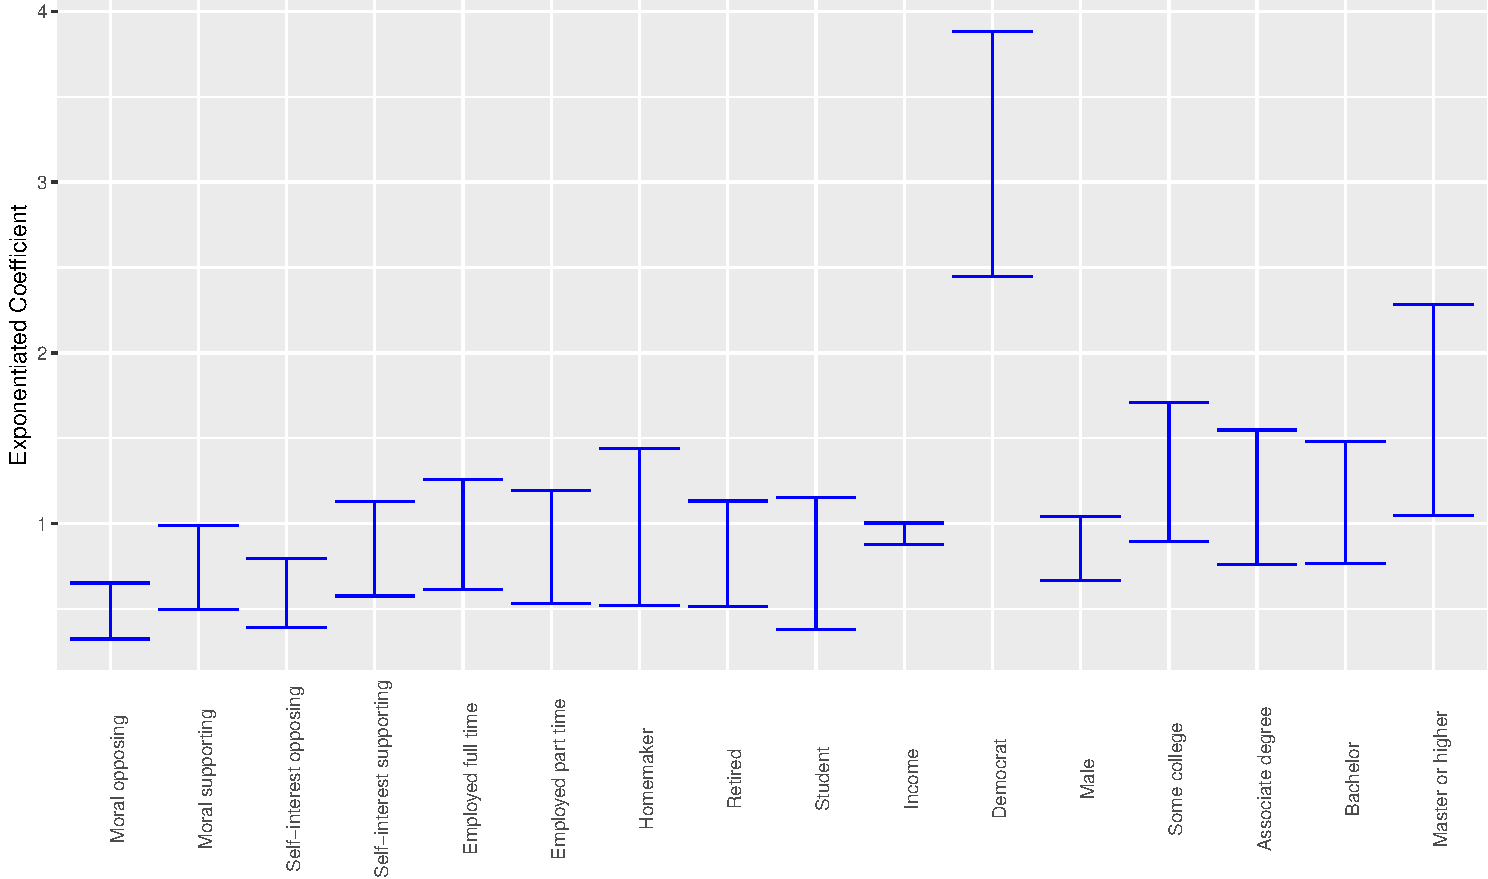
\includegraphics{dissertation_files/figure-latex/Scatterplot-Exponentiated-OP-HC-1.pdf}
\caption{\label{fig:Scatterplot-Exponentiated-OP-HC}Exponentiated Coefficients with Confidence Intervals. OP, Healthcare\label{ScatExpOpHc}}
\end{figure}
\begin{figure}
\centering
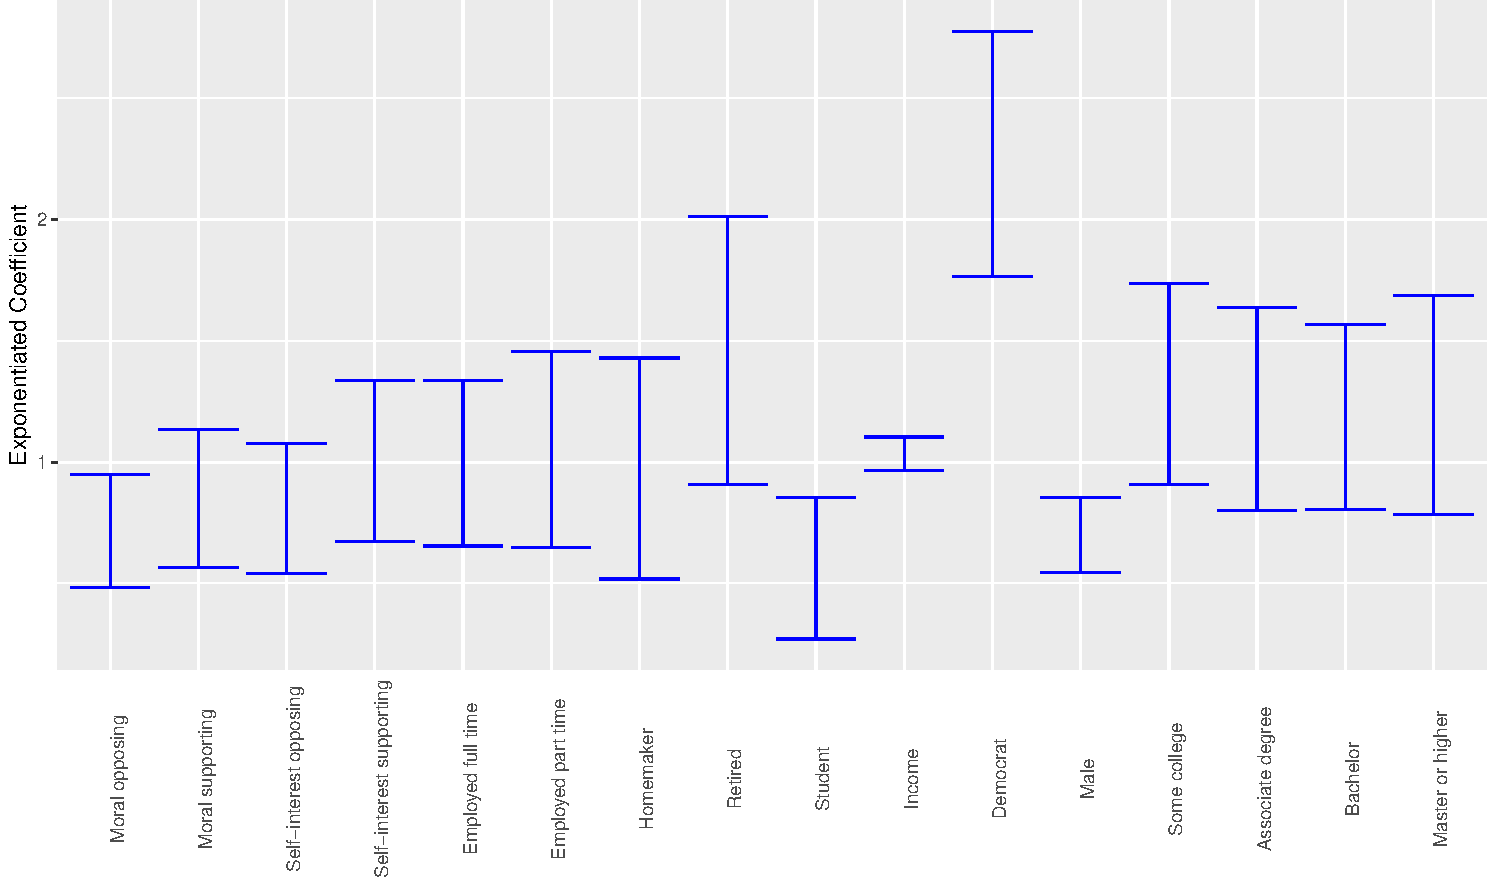
\includegraphics{dissertation_files/figure-latex/Scatterplot-Exponentiated-OP-EV-1.pdf}
\caption{\label{fig:Scatterplot-Exponentiated-OP-EV}Exponentiated Coefficients with Confidence Intervals. OP, Environment\label{ScatExpOpEv}}
\end{figure}
In the OP healthcare plot, for respondents who received the healthcare \texttt{Moral\ Opposing} frame, the odds of supporting the policy are between 35 and 67 percent lower than for respondents in other treatment groups. Similarly, the odds of supporting the OP environment policy for Democrats are between 1.8 and 2.8 times those of Republicans and Independents. The exponentiated estimates for the education categories in ANES environment are so large that they are excluded from Figure \ref{ScatExpAnEv} to make the other variables visible. There is no figure for ANES healthcare because the very high education coefficients did not allow exponentiated estimations.

The results between the two sets of education categories and the two issues differ markedly. There is a positive effect for Democrats across all regressions, but this is hardly surprising since the proposed policies in both issues lean towards liberalism. \texttt{Moral\ Opposing} also shows consistent results across ANES environment, OP healthcare, and OP environment. There is little consistency, however, regarding the other variables. \texttt{Income} only shows significant results for ANES healthcare, where wealthier respondents are more likely to oppose the policy. \texttt{Moral\ Supporting} shows significant results for ANES healthcare and OP healthcare, but the sign in the latter is negative. \texttt{Self-Interest\ Opposing} and \texttt{Master\ or\ higher} are only significant for OP healthcare, while \texttt{Male} only significantly decreases support for the OP environmental policy.

Overall, the \texttt{Moral\ Supporting} frames do not move people more towards supporting the issue policies than the self-interest frames. The ANES healthcare \texttt{Moral\ Supporting} frame does elicit a stronger positive effect than the corresponding \texttt{Self-Interest\ Supporting} frame, but the \texttt{Moral\ Supporting} frames for ANES environment and OP environment include the null. \texttt{Moral\ Supporting} for OP healthcare even shows statistically significant negative effects. There is some evidence, however, that \texttt{Moral\ Opposing} frames move people more towards opposing the issue policies than the \texttt{Self-Interest\ Opposing} frames. The \texttt{Moral\ Opposing} frames in ANES environment, OP environment, and OP healthcare all show statistically significant negative effects that are larger than their self-interest counterparts. One could thus argue that the results partially confirm \textbf{H1} for opposing frames. These results do not change when we account for the influence of party ID as a possible moderator (see appendix section \ref{app-framing-pid} for details).
\begin{figure}
\centering
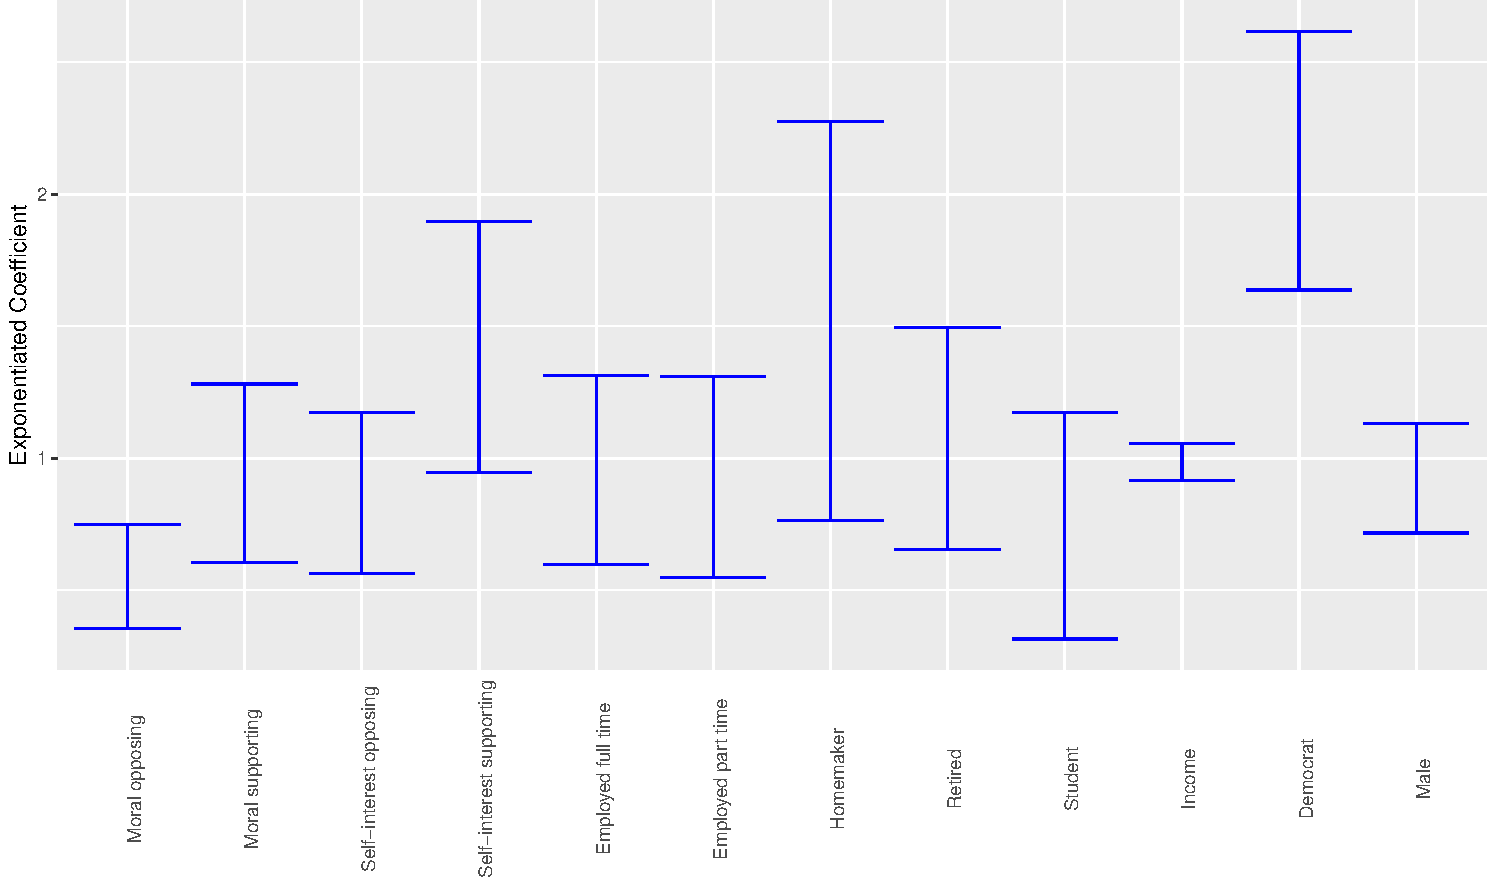
\includegraphics{dissertation_files/figure-latex/Scatterplot-Exponentiated-AN-EV-1.pdf}
\caption{\label{fig:Scatterplot-Exponentiated-AN-EV}Exponentiated Coefficients with Confidence Intervals. ANES, Environment\label{ScatExpAnEv}}
\end{figure}
\hypertarget{framing-results-experiment-mor-high}{%
\subsubsection{High Morality}\label{framing-results-experiment-mor-high}}

In order to create a collective measure of morality, I take the average of all morality question responses. This results in one overall morality score for each respondent. Respondents with high morality scores are defined as respondents with an average morality score in the top-third of the morality score distribution. Respondents with low morality scores are defined as respondents with an average morality score in the bottom-third of the morality score distribution. This results in groups of comparable sizes.

I run the same regression models as before after subsetting both data sets. Tables \ref{exp-hc-mor-high-low} and \ref{exp-ev-mor-high-low} show the results separated by issue. For healthcare, the confidence intervals for ANES high \texttt{Moral\ Opposing} and ANES low \texttt{Moral\ Opposing} include the null. ANES high \texttt{Moral\ Supporting} on the other hand is positive, while ANES low \texttt{Moral\ Supporting} again includes the null. \textbf{H2} claims that moral frames move people with higher morality scores more than people with lower morality scores. Based on the first finding, we fail to reject the null hypothesis for \textbf{H2}. Based on the second finding, however, we would reject it. This pattern continues for all estimates. For healthcare, OP high \texttt{Moral\ Opposing} is negative but OP low \texttt{Moral\ Opposing} includes the null, which means we would reject the null hypothesis. Both confidence intervals for OP high \texttt{Moral\ Supporting} and OP low \texttt{Moral\ Supporting} include zero, though, which means we would fail to reject the null hypothesis here. The same picture shows for environment: ANES high \texttt{Moral\ Opposing} is negative and ANES low \texttt{Moral\ Opposing} includes zero (i.e.~reject the NH), but both CIs for \texttt{Moral\ Supporting} include the null (i.e.~fail to reject the NH). Likewise, OP high \texttt{Moral\ Opposing} is negative and OP low \texttt{Moral\ Opposing} includes the null (i.e.~reject), while both CIs for \texttt{Moral\ Supporting} again include the null (i.e.~fail to reject). Results are thus mixed. The \texttt{Moral\ Opposing} frames appear to resonate more strongly with respondents with high morality scores, which would support \textbf{H2}, but the \texttt{Moral\ Supporting} frames mostly show null results, which would lead us to reject \textbf{H2}.

\ssp

\footnotesize

\blandscape
\centering
\captionof{table}{Ordinal Logistic Regression Results. High and Low Morality, Healthcare\label{exp-hc-mor-high-low}}
\begin{tabular}{@{\extracolsep{-60pt}}lD{.}{.}{-3} D{.}{.}{-3} D{.}{.}{-3} D{.}{.}{-3} } 
\\[-1.8ex]\hline 
\hline \\[-1.8ex] 
 & \multicolumn{4}{c}{\textit{Dependent variable:}} \\ 
\cline{2-5} 
\\[-1.8ex] & \multicolumn{4}{c}{Healthcare} \\ 
 & \multicolumn{1}{c}{ANES High} & \multicolumn{1}{c}{ANES Low} & \multicolumn{1}{c}{OP High} & \multicolumn{1}{c}{OP Low} \\ 
\hline \\[-1.8ex] 
 Moral opposing & -0.508$ $(-1.167$, $0.151) &0.205$ $(-0.513$, $0.923) & -1.132^{}$ $(-1.747$, $-0.517) & -0.467$ $(-1.084$, $0.150) \\ 
  Moral supporting &0.760^{}$ $(0.114$, $1.406) &0.510^{}$ $(-0.083$, $1.103) & -0.452$ $(-1.069$, $0.165) & -0.236$ $(-0.869$, $0.397) \\ 
  Self-interest opposing & -0.00002$ $(-0.600$, $0.600) &0.013$ $(-0.552$, $0.578) & -0.917^{}$ $(-1.553$, $-0.282) & -0.463$ $(-1.102$, $0.177) \\ 
  Self-interest supporting &0.023$ $(-0.620$, $0.667) &0.044$ $(-0.577$, $0.665) & -0.223$ $(-0.801$, $0.355) & -0.265$ $(-0.877$, $0.348) \\ 
  Employed full time &0.245$ $(-0.444$, $0.934) & -0.078$ $(-0.819$, $0.664) &0.182$ $(-0.469$, $0.834) & -0.317$ $(-0.964$, $0.330) \\ 
  Employed part time &0.352$ $(-0.450$, $1.153) & -0.036$ $(-0.832$, $0.759) &0.152$ $(-0.609$, $0.913) & -0.402$ $(-1.115$, $0.311) \\ 
  Homemaker &0.324$ $(-0.608$, $1.255) & -0.164$ $(-1.116$, $0.788) &0.523$ $(-0.326$, $1.373) & -0.815^{}$ $(-1.719$, $0.090) \\ 
  Retired & -0.487$ $(-1.177$, $0.204) & -0.304$ $(-1.164$, $0.556) & -0.257$ $(-0.910$, $0.396) & -0.321$ $(-1.094$, $0.451) \\ 
  Student &0.191$ $(-1.281$, $1.664) &0.291$ $(-0.756$, $1.338) & -0.967$ $(-2.299$, $0.365) & -0.411$ $(-1.330$, $0.508) \\ 
  Income & -0.107$ $(-0.237$, $0.023) & -0.104$ $(-0.234$, $0.026) & -0.146^{}$ $(-0.264$, $-0.028) &0.054$ $(-0.074$, $0.182) \\ 
  Democrat & 1.131^{}$ $(0.712$, $1.550) &0.695^{}$ $(0.264$, $1.127) & 1.490^{}$ $(1.072$, $1.907) &0.773^{}$ $(0.365$, $1.180) \\ 
  Male &0.324$ $(-0.101$, $0.748) &0.021$ $(-0.396$, $0.439) &0.141$ $(-0.273$, $0.555) & -0.086$ $(-0.484$, $0.311) \\ 
  1st-4th grade &  & 16.438^{}$ $(14.044$, $18.832) &  &  \\ 
  5th-6th grade &  & 17.453^{}$ $(15.031$, $19.875) &  &  \\ 
  7th-8th grade & -4.926^{}$ $(-7.867$, $-1.984) & 19.385^{}$ $(17.444$, $21.326) &  &  \\ 
  9th grade & -0.920$ $(-3.610$, $1.771) & 19.260^{}$ $(17.638$, $20.882) &  &  \\ 
  10th grade & -1.688$ $(-4.164$, $0.787) & 19.459^{}$ $(17.063$, $21.854) &  &  \\ 
  11th grade & 11.629^{}$ $(11.629$, $11.629) & 18.819^{}$ $(17.482$, $20.156) &  &  \\ 
  12th grade & -2.848^{}$ $(-4.849$, $-0.848) & 19.667^{}$ $(18.382$, $20.952) &  &  \\ 
  High school graduate & -1.336^{}$ $(-2.892$, $0.221) & 19.456^{}$ $(18.894$, $20.018) &  &  \\ 
  Some college & -1.391^{}$ $(-2.916$, $0.134) & 18.834^{}$ $(18.281$, $19.386) &0.123$ $(-0.438$, $0.684) & -0.241$ $(-0.807$, $0.326) \\ 
  Associate degree & -0.916$ $(-2.493$, $0.661) & 19.268^{}$ $(18.597$, $19.939) &0.322$ $(-0.281$, $0.926) & -0.307$ $(-0.927$, $0.313) \\ 
  Bachelor & -1.481^{}$ $(-2.982$, $0.020) & 19.302^{}$ $(18.700$, $19.904) &0.213$ $(-0.372$, $0.798) & -0.369$ $(-0.974$, $0.235) \\ 
  Master & -1.158$ $(-2.765$, $0.449) & 19.332^{}$ $(18.647$, $20.017) &  &  \\ 
  Professional degree & -0.907$ $(-3.230$, $1.415) & 18.767^{}$ $(17.809$, $19.726) &  &  \\ 
  Doctorate &  & 19.392^{}$ $(18.302$, $20.482) &  &  \\ 
  Master or higher &  &  &0.747^{}$ $(0.001$, $1.492) & -0.084$ $(-0.793$, $0.626) \\ 
 \hline \\[-1.8ex] 
Observations & \multicolumn{1}{c}{354} & \multicolumn{1}{c}{354} & \multicolumn{1}{c}{367} & \multicolumn{1}{c}{368} \\ 
\hline \\[-1.8ex] 
\end{tabular}
\fillandplacepagenumber
\elandscape

\dsp

\normalsize

\ssp

\footnotesize

\blandscape
\centering
\captionof{table}{Ordinal Logistic Regression Results. High and Low Morality, Environment\label{exp-ev-mor-high-low}}
\begin{tabular}{@{\extracolsep{-60pt}}lD{.}{.}{-3} D{.}{.}{-3} D{.}{.}{-3} D{.}{.}{-3} } 
\\[-1.8ex]\hline 
\hline \\[-1.8ex] 
 & \multicolumn{4}{c}{\textit{Dependent variable:}} \\ 
\cline{2-5} 
\\[-1.8ex] & \multicolumn{4}{c}{Environment} \\ 
 & \multicolumn{1}{c}{ANES High} & \multicolumn{1}{c}{ANES Low} & \multicolumn{1}{c}{OP High} & \multicolumn{1}{c}{OP Low} \\ 
\hline \\[-1.8ex] 
 Moral opposing & -1.059^{}$ $(-1.706$, $-0.412) & -0.142$ $(-0.787$, $0.503) & -0.987^{}$ $(-1.613$, $-0.360) &0.200$ $(-0.405$, $0.805) \\ 
  Moral supporting & -0.333$ $(-1.017$, $0.351) &0.409$ $(-0.264$, $1.083) & -0.355$ $(-0.974$, $0.263) &0.285$ $(-0.335$, $0.906) \\ 
  Self-interest opposing & -0.121$ $(-0.780$, $0.538) &0.110$ $(-0.582$, $0.801) & -0.674^{}$ $(-1.283$, $-0.065) &0.163$ $(-0.453$, $0.780) \\ 
  Self-interest supporting &0.237$ $(-0.370$, $0.844) &0.732^{}$ $(0.087$, $1.377) & -0.606^{}$ $(-1.257$, $0.045) &0.649^{}$ $(0.029$, $1.270) \\ 
  Employed full time & -0.194$ $(-0.893$, $0.504) &0.067$ $(-0.647$, $0.781) &0.274$ $(-0.381$, $0.928) & -0.574^{}$ $(-1.219$, $0.071) \\ 
  Employed part time &0.237$ $(-0.597$, $1.071) & -0.019$ $(-0.787$, $0.749) &0.641^{}$ $(-0.104$, $1.387) & -0.797^{}$ $(-1.520$, $-0.075) \\ 
  Homemaker &0.510$ $(-0.450$, $1.470) &0.446$ $(-0.518$, $1.410) &0.496$ $(-0.368$, $1.359) & -0.884^{}$ $(-1.779$, $0.011) \\ 
  Retired & -0.329$ $(-1.027$, $0.370) & -0.059$ $(-0.884$, $0.766) &0.533$ $(-0.137$, $1.203) &0.179$ $(-0.582$, $0.940) \\ 
  Student & -0.507$ $(-2.029$, $1.015) &0.153$ $(-0.903$, $1.209) & -0.202$ $(-1.635$, $1.230) & -1.149^{}$ $(-2.096$, $-0.201) \\ 
  Income & -0.058$ $(-0.193$, $0.078) &0.006$ $(-0.122$, $0.134) &0.064$ $(-0.056$, $0.183) &0.100$ $(-0.026$, $0.225) \\ 
  Democrat &0.674^{}$ $(0.262$, $1.085) &0.295$ $(-0.133$, $0.722) &0.996^{}$ $(0.591$, $1.400) &0.331$ $(-0.070$, $0.732) \\ 
  Male &0.190$ $(-0.235$, $0.616) &0.035$ $(-0.378$, $0.447) &0.108$ $(-0.312$, $0.529) & -0.427^{}$ $(-0.834$, $-0.021) \\ 
  1st-4th grade &  &0.569$ $(-4.455$, $5.594) &  &  \\ 
  5th-6th grade &  & -0.191$ $(-5.112$, $4.730) &  &  \\ 
  7th-8th grade & -0.751$ $(-4.618$, $3.116) & 1.376$ $(-3.476$, $6.228) &  &  \\ 
  9th grade &0.125$ $(-3.216$, $3.465) & -0.529$ $(-5.271$, $4.214) &  &  \\ 
  10th grade &0.231$ $(-2.279$, $2.740) &0.033$ $(-4.892$, $4.958) &  &  \\ 
  11th grade &0.729$ $(-2.431$, $3.888) &0.221$ $(-4.531$, $4.973) &  &  \\ 
  12th grade & -0.041$ $(-2.081$, $1.999) & -0.067$ $(-4.690$, $4.555) &  &  \\ 
  High school graduate &0.492$ $(-1.103$, $2.087) &0.684$ $(-3.757$, $5.125) &  &  \\ 
  Some college &0.919$ $(-0.649$, $2.487) &0.709$ $(-3.731$, $5.150) &0.309$ $(-0.254$, $0.873) & -0.346$ $(-0.915$, $0.223) \\ 
  Associate degree &0.854$ $(-0.766$, $2.474) &0.918$ $(-3.534$, $5.370) &0.152$ $(-0.465$, $0.769) & -0.036$ $(-0.662$, $0.589) \\ 
  Bachelor & 1.190$ $(-0.348$, $2.728) &0.761$ $(-3.667$, $5.189) &0.306$ $(-0.301$, $0.913) & -0.315$ $(-0.906$, $0.276) \\ 
  Master & 1.569^{}$ $(-0.064$, $3.201) &0.544$ $(-3.899$, $4.986) &  &  \\ 
  Professional degree & 1.397$ $(-0.940$, $3.734) &0.815$ $(-3.694$, $5.323) &  &  \\ 
  Doctorate &  &0.790$ $(-3.743$, $5.322) &  &  \\ 
  Master or higher &  &  & -0.144$ $(-0.853$, $0.564) & -0.161$ $(-0.879$, $0.558) \\ 
 \hline \\[-1.8ex] 
Observations & \multicolumn{1}{c}{354} & \multicolumn{1}{c}{354} & \multicolumn{1}{c}{367} & \multicolumn{1}{c}{368} \\ 
\hline \\[-1.8ex] 
\end{tabular}
\fillandplacepagenumber
\elandscape

\dsp

\normalsize

\hypertarget{framing-results-experiment-si-high}{%
\subsubsection{High Self-Interest}\label{framing-results-experiment-si-high}}

The collective measure of self-interest is created in the same way as the above collective measure of morality. I take the average of all self-interest question responses, resulting in one overall self-interest score for each respondent. Respondents with high self-interest scores are defined as respondents with an average self-interest score in the top-third of the self-interest score distribution. Respondents with low self-interest scores are defined as respondents with an average self-interest score in the bottom-third of the self-interest score distribution. This again results in groups of comparable sizes.

As above, I run the same regression models as before after subsetting both data sets. Tables \ref{exp-hc-si-high-low} and \ref{exp-ev-si-high-low} show the results separated by issue. While the evidence for high and low morality (\textbf{H2}) was mixed, with some results indicating the ability to reject the null hypothesis, this is not the case for self-interest. None of the results for any self-interest group for any data set for any issue show evidence that self-interest frames move people with higher self-interest scores more than people with lower self-interest scores, as \textbf{H3} asserts. Only two self-interest results are statistically significant, namely healthcare OP High \texttt{Self-Interest\ Opposing} and OP Low \texttt{Self-Interest\ Opposing}. Both coefficients show the expected negative sign, but the negative effect is larger for OP Low (-0.706 vs.~-0.666). This appears to support the theory that the \texttt{Self-Interest\ Oppsing} frame resonates more strongly with respondents with low self-interest scores. I thus fail to reject the null hypothesis for \textbf{H3}.

\ssp

\footnotesize

\blandscape
\centering
\captionof{table}{Ordinal Logistic Regression Results. High and Low Self-Interest, Healthcare\label{exp-hc-si-high-low}}
\begin{tabular}{@{\extracolsep{-60pt}}lD{.}{.}{-3} D{.}{.}{-3} D{.}{.}{-3} D{.}{.}{-3} } 
\\[-1.8ex]\hline 
\hline \\[-1.8ex] 
 & \multicolumn{4}{c}{\textit{Dependent variable:}} \\ 
\cline{2-5} 
\\[-1.8ex] & \multicolumn{4}{c}{Healthcare} \\ 
 & \multicolumn{1}{c}{ANES High} & \multicolumn{1}{c}{ANES Low} & \multicolumn{1}{c}{OP High} & \multicolumn{1}{c}{OP Low} \\ 
\hline \\[-1.8ex] 
 Moral opposing &0.024$ $(-0.634$, $0.682) & -0.275$ $(-0.950$, $0.401) & -0.877^{}$ $(-1.526$, $-0.229) & -0.752^{}$ $(-1.352$, $-0.153) \\ 
  Moral supporting &0.396$ $(-0.220$, $1.013) &0.478$ $(-0.176$, $1.132) & -0.699^{}$ $(-1.307$, $-0.090) & -0.488$ $(-1.099$, $0.123) \\ 
  Self-interest opposing &0.203$ $(-0.419$, $0.825) & -0.024$ $(-0.594$, $0.547) & -0.666^{}$ $(-1.296$, $-0.036) & -0.706^{}$ $(-1.308$, $-0.104) \\ 
  Self-interest supporting &0.261$ $(-0.374$, $0.895) &0.227$ $(-0.407$, $0.862) & -0.576^{}$ $(-1.166$, $0.015) & -0.014$ $(-0.613$, $0.584) \\ 
  Employed full time & -0.368$ $(-1.059$, $0.323) &0.176$ $(-0.503$, $0.855) & -0.221$ $(-0.837$, $0.395) & -0.290$ $(-0.935$, $0.355) \\ 
  Employed part time & -0.013$ $(-0.747$, $0.721) & -0.318$ $(-1.125$, $0.489) & -0.013$ $(-0.694$, $0.669) & -0.501$ $(-1.229$, $0.227) \\ 
  Homemaker &0.151$ $(-0.918$, $1.220) & -0.081$ $(-0.916$, $0.755) &0.186$ $(-0.969$, $1.341) & -0.063$ $(-0.875$, $0.749) \\ 
  Retired & -0.242$ $(-1.002$, $0.519) & -0.062$ $(-0.771$, $0.648) &0.269$ $(-0.504$, $1.042) & -0.658^{}$ $(-1.314$, $-0.002) \\ 
  Student & -0.310$ $(-1.385$, $0.765) &0.124$ $(-1.160$, $1.409) & -0.351$ $(-1.277$, $0.576) & -0.976^{}$ $(-2.040$, $0.087) \\ 
  Income & -0.001$ $(-0.125$, $0.124) & -0.104$ $(-0.234$, $0.027) &0.082$ $(-0.036$, $0.201) & -0.113^{}$ $(-0.230$, $0.004) \\ 
  Democrat & 1.173^{}$ $(0.748$, $1.599) & 1.002^{}$ $(0.582$, $1.423) & 1.105^{}$ $(0.699$, $1.511) & 1.670^{}$ $(1.244$, $2.096) \\ 
  Male & -0.115$ $(-0.539$, $0.309) &0.050$ $(-0.379$, $0.478) & -0.398^{}$ $(-0.803$, $0.008) &0.002$ $(-0.395$, $0.399) \\ 
  7th-8th grade & -18.900^{}$ $(-18.900$, $-18.900) & 22.434^{}$ $(19.581$, $25.286) &  &  \\ 
  9th grade &0.497$ $(-1.712$, $2.706) & 22.054^{}$ $(19.207$, $24.901) &  &  \\ 
  10th grade & 1.323$ $(-1.727$, $4.373) & 23.931^{}$ $(22.157$, $25.705) &  &  \\ 
  11th grade &0.002$ $(-2.335$, $2.340) & 22.255^{}$ $(20.560$, $23.950) &  &  \\ 
  12th grade & -0.311$ $(-2.375$, $1.753) & 22.217^{}$ $(21.049$, $23.384) &  &  \\ 
  High school graduate &0.213$ $(-1.084$, $1.510) & 22.935^{}$ $(22.364$, $23.506) &  &  \\ 
  Some college &0.221$ $(-1.055$, $1.497) & 22.687^{}$ $(22.117$, $23.256) &0.347$ $(-0.242$, $0.937) &0.149$ $(-0.401$, $0.700) \\ 
  Associate degree & -0.136$ $(-1.468$, $1.195) & 23.078^{}$ $(22.440$, $23.716) & -0.009$ $(-0.645$, $0.626) &0.329$ $(-0.306$, $0.964) \\ 
  Bachelor & -0.044$ $(-1.293$, $1.206) & 22.900^{}$ $(22.269$, $23.531) & -0.215$ $(-0.811$, $0.381) &0.290$ $(-0.281$, $0.861) \\ 
  Master & -0.181$ $(-1.474$, $1.113) & 22.999^{}$ $(22.250$, $23.748) &  &  \\ 
  Professional degree &0.195$ $(-1.376$, $1.766) & 22.055^{}$ $(20.564$, $23.546) &  &  \\ 
  Doctorate &  & 23.211^{}$ $(21.822$, $24.600) &  &  \\ 
  Master or higher &  &  &0.415$ $(-0.254$, $1.083) &0.395$ $(-0.287$, $1.077) \\ 
 \hline \\[-1.8ex] 
Observations & \multicolumn{1}{c}{354} & \multicolumn{1}{c}{354} & \multicolumn{1}{c}{367} & \multicolumn{1}{c}{368} \\ 
\hline \\[-1.8ex] 
\end{tabular} 
\fillandplacepagenumber
\elandscape

\dsp

\normalsize

\ssp

\footnotesize

\blandscape
\centering
\captionof{table}{Ordinal Logistic Regression Results. High and Low Self-Interest, Environment\label{exp-ev-si-high-low}}
\begin{tabular}{@{\extracolsep{-60pt}}lD{.}{.}{-3} D{.}{.}{-3} D{.}{.}{-3} D{.}{.}{-3} } 
\\[-1.8ex]\hline 
\hline \\[-1.8ex] 
 & \multicolumn{4}{c}{\textit{Dependent variable:}} \\ 
\cline{2-5} 
\\[-1.8ex] & \multicolumn{4}{c}{Environment} \\ 
 & \multicolumn{1}{c}{ANES High} & \multicolumn{1}{c}{ANES Low} & \multicolumn{1}{c}{OP High} & \multicolumn{1}{c}{OP Low} \\ 
\hline \\[-1.8ex] 
 Moral opposing & -0.346$ $(-1.019$, $0.328) & -0.672^{}$ $(-1.322$, $-0.022) & -0.970^{}$ $(-1.579$, $-0.362) & -0.484$ $(-1.074$, $0.106) \\ 
  Moral supporting &0.435$ $(-0.248$, $1.118) & -0.144$ $(-0.785$, $0.498) & -0.999^{}$ $(-1.620$, $-0.378) &0.201$ $(-0.439$, $0.840) \\ 
  Self-interest opposing & -0.118$ $(-0.779$, $0.543) & -0.127$ $(-0.794$, $0.539) & -0.600^{}$ $(-1.239$, $0.040) & -0.246$ $(-0.851$, $0.359) \\ 
  Self-interest supporting &0.564^{}$ $(-0.063$, $1.192) &0.116$ $(-0.495$, $0.726) & -0.476$ $(-1.087$, $0.134) & -0.008$ $(-0.608$, $0.592) \\ 
  Employed full time & -0.513$ $(-1.188$, $0.162) &0.050$ $(-0.638$, $0.737) & -0.248$ $(-0.883$, $0.386) &0.258$ $(-0.372$, $0.888) \\ 
  Employed part time & -0.655^{}$ $(-1.384$, $0.074) & -0.055$ $(-0.853$, $0.743) &0.071$ $(-0.627$, $0.768) &0.155$ $(-0.572$, $0.881) \\ 
  Homemaker &0.404$ $(-0.691$, $1.499) & -0.069$ $(-0.938$, $0.801) & -0.620$ $(-1.745$, $0.506) &0.025$ $(-0.777$, $0.827) \\ 
  Retired & -0.643^{}$ $(-1.375$, $0.089) &0.239$ $(-0.475$, $0.954) &0.067$ $(-0.741$, $0.875) &0.291$ $(-0.353$, $0.934) \\ 
  Student & -0.789$ $(-1.895$, $0.318) & -0.710$ $(-2.000$, $0.581) & -0.535$ $(-1.495$, $0.425) & -0.346$ $(-1.437$, $0.746) \\ 
  Income &0.063$ $(-0.062$, $0.188) & -0.010$ $(-0.140$, $0.119) &0.127^{}$ $(0.009$, $0.244) & -0.034$ $(-0.151$, $0.083) \\ 
  Democrat &0.836^{}$ $(0.417$, $1.254) &0.607^{}$ $(0.188$, $1.026) &0.678^{}$ $(0.282$, $1.073) &0.962^{}$ $(0.552$, $1.372) \\ 
  Male &0.090$ $(-0.332$, $0.513) & -0.004$ $(-0.430$, $0.421) & -0.603^{}$ $(-1.012$, $-0.194) & -0.189$ $(-0.595$, $0.216) \\ 
  7th-8th grade & -17.009^{}$ $(-17.009$, $-17.009) &0.388$ $(-4.562$, $5.339) &  &  \\ 
  9th grade & -1.176$ $(-3.362$, $1.009) & -16.327^{}$ $(-16.327$, $-16.327) &  &  \\ 
  10th grade & -2.583^{}$ $(-5.124$, $-0.041) & 3.193$ $(-1.352$, $7.737) &  &  \\ 
  11th grade &0.146$ $(-2.148$, $2.439) &0.269$ $(-4.027$, $4.565) &  &  \\ 
  12th grade & -0.462$ $(-2.765$, $1.841) &0.506$ $(-3.587$, $4.599) &  &  \\ 
  High school graduate & -0.082$ $(-1.394$, $1.231) &0.728$ $(-3.204$, $4.661) &  &  \\ 
  Some college &0.060$ $(-1.250$, $1.371) & 1.299$ $(-2.629$, $5.227) &0.334$ $(-0.281$, $0.949) &0.043$ $(-0.508$, $0.593) \\ 
  Associate degree & -0.187$ $(-1.558$, $1.185) & 1.508$ $(-2.429$, $5.446) & -0.022$ $(-0.676$, $0.632) &0.405$ $(-0.215$, $1.026) \\ 
  Bachelor & -0.032$ $(-1.309$, $1.244) & 1.643$ $(-2.274$, $5.560) & -0.030$ $(-0.641$, $0.581) & -0.116$ $(-0.706$, $0.474) \\ 
  Master &0.106$ $(-1.219$, $1.431) & 1.225$ $(-2.705$, $5.156) &  &  \\ 
  Professional degree &0.031$ $(-1.541$, $1.602) & -0.058$ $(-4.224$, $4.107) &  &  \\ 
  Doctorate &  &0.676$ $(-3.389$, $4.740) &  &  \\ 
  Master or higher &  &  &0.204$ $(-0.462$, $0.871) & -0.147$ $(-0.823$, $0.530) \\ 
 \hline \\[-1.8ex] 
Observations & \multicolumn{1}{c}{354} & \multicolumn{1}{c}{354} & \multicolumn{1}{c}{367} & \multicolumn{1}{c}{368} \\ 
\hline \\[-1.8ex] 
\end{tabular}
\fillandplacepagenumber
\elandscape

\dsp

\normalsize

\clearpage

\hypertarget{framing-results-experiment-imputation}{%
\subsection{Imputation}\label{framing-results-experiment-imputation}}

\vspace{-9cm}

As mentioned above, both methods from the previous chapters are applied in the fielding and analysis of the experiment. The ordered probit blocking method from chapter \ref{ordblock} was used to block respondents into treatment groups based on two differing sets of education categories (ANES and OP). This section now applies the ordinal variable imputation method developed in chapter \ref{ordmiss} to both sets of data from the experiment. As in chapter \ref{ordmiss}, I artificially insert missing values and subsequently impute the missing data with four different imputation methods: \texttt{hot.deck} from the \texttt{hot.deck} package, \texttt{amelia} from the \texttt{Amelia} package, \texttt{mice} from the \texttt{mice} package, and my self-penned method \texttt{hd.ord} which is specifically designed for ordinal variables. As before, I also include list-wise deletion with \texttt{na.omit}. Since we know the true values for each imputed variable, we can assess which method comes closest to the truth and thus performs best. As in chapter \ref{ordmiss}, the analysis is conducted for two missing data mechanisms, MAR and MNAR. Each data set is imputed 1,000 times with each of the four imputation methods. 20 percent missing values are randomly amputed in each iteration for each data set. As in the preceding sections of this chapter, the analysis is split into ANES and OP sets of education categories. As before, missing data is amputed for five variables.

With data missing at random in the ANES set (Table \ref{mar.5var.frame}), \texttt{hd.ord} performs worse than \texttt{amelia} and \texttt{mice} but on par with \texttt{hot.deck} for the three binary variables \texttt{Democrat}, \texttt{Male} and \texttt{Employed}. \texttt{hd.ord} is furthest away from the true value for the interval variables \texttt{Income} (--0.0113) and \texttt{Age} (--0.3107), with the exception of \texttt{na.omit}.

\ssp
\begin{table}[H] \centering  
 \caption{Accuracy of Multiple Imputation Methods. Framing Data, MAR, 5 Variables with NA}   
 \label{mar.5var.frame} 
\begin{threeparttable}
 \begin{tabular}{ccr@{}lr@{}l} 
 \\[-1.8ex]\hline 
 \hline \\[-1.8ex] 
 \multicolumn{1}{c}{Method} & \multicolumn{1}{c}{Variable} & \multicolumn{2}{c}{ANES} & \multicolumn{2}{c}{OP} \\
 \hline \\[-1.8ex]
 true & Democrat & 0.&3879 & 0.&3826 \\ 
 hot.deck & Democrat & +0.&0006 & +0.&0005 \\
 hd.ord & Democrat & +0.&0007 & +0.&0004 \\
 amelia & Democrat & +0.&0001 & --0.&0001 \\
 mice & Democrat & +0.&0001 & --0.&0001 \\
 na.omit & Democrat & --0.&0313 & --0.&0343 \\ 
 true & Male & 0.&4576 & 0.&4714 \\ 
 hot.deck & Male & +0.&0008 & +0.&0013 \\
 hd.ord & Male & +0.&0005 & +0.&0013 \\
 amelia & Male & +0.&0001 & +0.&0000 \\
 mice & Male & +0.&0000 & --0.&0001 \\ 
 na.omit & Male & --0.&0429 & --0.&0421 \\ 
 true & Employed & 0.&5612 & 0.&5684 \\ 
 hot.deck & Employed & +0.&0012 & +0.&0012 \\
 hd.ord & Employed & +0.&0013 & +0.&0013 \\
 amelia & Employed & +0.&0002 & +0.&0001 \\ 
 mice & Employed & --0.&0001 & --0.&0001 \\
 na.omit & Employed & --0.&0353 & --0.&0358 \\
 true & Income & 3.&5537 & 3.&4923 \\
 hot.deck & Income & --0.&0047 & --0.&0026 \\
 hd.ord & Income & --0.&0113 & --0.&0107 \\ 
 amelia & Income & --0.&0004 & --0.&0017 \\ 
 mice & Income & --0.&0014 & --0.&0016 \\ 
 na.omit & Income & --0.&1924 & --0.&1958 \\
 true & Age & 46.&3475 & 44.&9574 \\
 hot.deck & Age & --0.&1621 & --0.&1711 \\ 
 hd.ord & Age & --0.&3107 & --0.&2837 \\
 amelia & Age & --0.&0009 & +0.&0040 \\
 mice & Age & --0.&0073 & +0.&0000 \\ 
 na.omit & Age & --0.&8376 & --0.&8373 \\
 \hline \\[-1.8ex] 
\end{tabular} 
\begin{tablenotes}[para,flushleft]
\footnotesize{\textit{Note:} Each \texttt{true} value shows the true variable mean. All other values show the differences between the imputation means and the true mean, indicated with a + or -- sign.}
\end{tablenotes}
\end{threeparttable}
\end{table}
\begin{table}[H] \centering 
 \caption{Accuracy of Multiple Imputation Methods. Framing Data, MNAR, 5 Variables with NA}  
 \label{mnar.5var.frame}  
 \begin{threeparttable}
\begin{tabular}{ccr@{}lr@{}l} 
 \\[-1.8ex]\hline 
 \hline \\[-1.8ex]
 \multicolumn{1}{c}{Method} & \multicolumn{1}{c}{Variable} & \multicolumn{2}{c}{ANES} & \multicolumn{2}{c}{OP} \\
 \hline \\[-1.8ex] 
 true & Democrat & 0.&3879 & 0.&3826 \\
 hot.deck & Democrat & --0.&0035 & --0.&0031 \\ 
 hd.ord & Democrat & --0.&0039 & --0.&0039 \\
 amelia & Democrat & --0.&0034 & --0.&0032 \\
 mice & Democrat & --0.&0028 & --0.&0028 \\ 
 na.omit & Democrat & --0.&0188 & --0.&0197 \\ 
 true & Male & 0.&4576 & 0.&4714 \\
 hot.deck & Male & --0.&0138 & --0.&0127 \\
 hd.ord & Male & --0.&0134 & --0.&0124 \\
 amelia & Male & --0.&0137 & --0.&0133 \\
 mice & Male & --0.&0138 & --0.&0136 \\
 na.omit & Male & --0.&0231 & --0.&0220 \\
 true & Employed & 0.&5612 & 0.&5684 \\
 hot.deck & Employed & --0.&0027 & --0.&0028 \\
 hd.ord & Employed & --0.&0030 & --0.&0034 \\
 amelia & Employed & --0.&0031 & --0.&0030 \\
 mice & Employed & --0.&0030 & --0.&0030 \\
 na.omit & Employed & --0.&0180 & --0.&0178 \\
 true & Income & 3.&5537 & 3.&4923 \\
 hot.deck & Income & --0.&0498 & --0.&0480 \\
 hd.ord & Income & --0.&0528 & --0.&0541 \\ 
 amelia & Income & --0.&0413 & --0.&0439 \\ 
 mice & Income & --0.&0415 & --0.&0441 \\ 
 na.omit & Income & --0.&1064 & --0.&1043 \\
 true & Age & 46.&3475 & 44.&9574 \\ 
 hot.deck & Age & --0.&4322 & --0.&4795 \\
 hd.ord & Age & --0.&6215 & --0.&5925 \\
 amelia & Age & --0.&2420 & --0.&2725 \\ 
 mice & Age & --0.&2441 & --0.&2768 \\ 
 na.omit & Age & --0.&5301 & --0.&5076 \\
 \hline \\[-1.8ex] 
\end{tabular} 
\begin{tablenotes}[para,flushleft]
\footnotesize{\textit{Note:} Each \texttt{true} value shows the true variable mean. All other values show the differences between the imputation means and the true mean, indicated with a + or -- sign.}
\end{tablenotes}
\end{threeparttable}
\end{table}
\dsp

While \texttt{mice} and \texttt{amelia} perform equally well for the binary variables, \texttt{amelia} shows a markedly better performance for the interval variables. The results for the OP data mirror the ANES results for \texttt{hot.deck} and \texttt{hd.ord}. They show the same levels of distances for the binary variables and \texttt{hd.ord} performs markedly worse for the interval variables. Notably, however, \texttt{mice} is not inferior to \texttt{amelia} for the interval variables in the OP data. \texttt{mice} actually beats \texttt{amelia} for \texttt{Age}, which is a striking reversal of the ANES results.\footnote{For a repeat of this MAR analysis for 10 amputed variables, see appendix section \ref{app-framing-10var}. The results do not change substantively.}

All imputation results for data MNAR (Table \ref{mnar.5var.frame}) are much further away from the true values than in Table \ref{mar.5var.frame}. This is to be expected given the differing missing data mechanisms. The pattern for MNAR is markedly different: \texttt{hot.deck} and \texttt{hd.ord} show virtually identical results as \texttt{amelia} and \texttt{mice} for the binary variables for both data sets. \texttt{hd.ord} even performs best among all mechanisms for \texttt{Male}. While \texttt{amelia} and \texttt{mice} still produce significantly closer results for \texttt{Income} and \texttt{Age}, the distance to the two hot decking methods is notably smaller. Between the two hot decking methods, however, \texttt{hd.ord} comes last. \texttt{hd.ord} in fact performs worse than \texttt{na.omit} for \texttt{Age} in both data sets.\footnote{For a repeat of this MNAR analysis for 10 amputed variables, see appendix section \ref{app-framing-10var}. The results do not change substantively.}

\hypertarget{framing-conclusion}{%
\section{Conclusion}\label{framing-conclusion}}

I set out to test the influence of morality and self-interest in political framing and to investigate how morality and self-interest contribute to persuasive strength in emphasis frames. Morality was defined along the lines of Moral Foundations Theory with a focus on the foundation of Care/Harm, while self-interest was considered to cover the areas of personal autonomy, health/safety, wealth, and status. I designed a survey experiment that measured respondents' morality and self-interest attitudes and applied my self-penned ordered probit method to block each respondent on the basis of their education (ANES, OP) into one of five treatment groups (\texttt{Moral\ opposing}, \texttt{Moral\ supporting}, \texttt{Self-interest\ opposing}, \texttt{Self-interest\ supporting}, and \texttt{Control}) for two political issues (healthcare, environment). On the basis of the asserted strength of moral arguments due to their deep connection with emotions and the corresponding lack of strength of non-moral arguments, I hypothesized that moral frames move respondents more than self-interest frames (\textbf{H1}). I further hypothesized that the effect of different frames should be felt differently conditional on respondents' own morality and self-interest priorities. A moral frame should affect respondents' opinion more if they score highly on the morality measures as this type of frame is likely to connect more with their values (\textbf{H2}). Correspondingly, a self-interest frame should register more with respondents' opinion if they score highly on the self-interest measures (\textbf{H3}). Finally, I tested the effectiveness of my developed ordinal variable imputation method by artificially inserting missing data.

The results are mixed. \textbf{H1} is partially confirmed for opposing frames. There is evidence that \texttt{Moral\ Opposing} frames move people more towards opposing the issue policies than \texttt{Self-Interest\ Opposing} frames. The \texttt{Moral\ Opposing} frames for ANES environment, OP environment, and OP healthcare all show statistically significant negative effects that are larger than their self-interest counterparts. The same does not hold for \texttt{Moral\ Supporting} frames. Most of the corresponding regression confidence intervals here include the null of no treatment effect. \textbf{H2} is also partially confirmed for opposing frames. The \texttt{Moral\ Opposing} frames appear to resonate more strongly with respondents with high morality scores for both issues, but the \texttt{Moral\ Supporting} frames do not elicit a treatment effect. \textbf{H3}, however, is not confirmed. None of the results for any self-interest group for any data set for any issue show any evidence that self-interest frames move people with higher self-interest scores more than people with lower self-interest scores.

The missing data analysis confirms the results from chapter \ref{ordmiss}. \texttt{hd.ord} does not perform on the level of \texttt{amelia}, particularly for non-binary variables. The gap to \texttt{amelia} is narrower for imputations carried out for data MNAR, but this does not change the overall results.

It is unclear why the \texttt{Moral\ Opposing} frames confirm the hypotheses while the \texttt{Moral\ Supporting} ones do not. One possible explanation could be differences in the level of frame wording. It could be that the \texttt{Moral\ Opposing} categories are surreptitiously worded more effectively than their supporting counterparts. This seems unlikely, though, as the results for \texttt{Moral\ Opposing} frames are consistent across both issues. Another potential area of investigation could be the juxtaposition of negativity and positivity. Perhaps it is easier and clearer for people to establish what they are morally against than what they morally support. What I dislike, i.e.~negative morality, might be easier to figure out than the things I stand for.

One final aspect is notable: The sheer number of ANES education categories renders ordinal logistic regressions difficult. These finely grated and overly nuanced categories often result in a low number of observations per category. This greatly increases regression coefficients, which makes interpretation cumbersome and sometimes impossible, e.g.~when exponentiated coefficients can not be calculated for ANES healthcare. The large number of ANES education categories also leads to frequent collinearity, causing the models to drop variable levels. None of this occurs with the OP education categories, which raises doubt about the necessity for such finely separated categories.

\hypertarget{conclusion}{%
\chapter{CONCLUSION}\label{conclusion}}

Education is one of the most important predictors of political behavior in political science. As an ordinal variable, education possesses special characteristics: Its categories are ordered, but unevenly spaced. It is crucial that we try to use this unique information to the greatest extent possible. If we want to know what people think and how they act, we need to make sure our measurements are as good as they can possibly be. The ordered probit approach I outlined and applied in the previous chapters represents an attempt to do so. While there are some encouraging signs, the overall conclusion after these analyses speaks against an endorsement of this approach. Assuming a latent underlying continuous variable underneath education, estimating cutoff thresholds between the education categories, and binning observations according to linear model predictors to obtain a new set of education categories based on data fit overall does not appear to improve upon current research practice.

Blocking on the two differing education sets (ANES and OP) shows mixed results. While an ANOVA regression of the numerical variables does not result in statistically distinct intercepts, a similar general linear model reveals statistical significance for most of the factor variables. The distributions of the placebo regression treatment variables appear to indicate slightly superior performance by the OP method, but this evidence is tentative because of the sample size. It is thus overall unclear whether the re-estimation of ordinal variable categories with an ordered probit approach matters for the process of blocking.

The verdict is much clearer for multiple hot deck imputation with ordinal variables. Adapting the multiple hot deck imputation function \texttt{hot.deck} to treat ordinal variables with an ordered probit model does not improve on current methods. \texttt{hd.ord} performs on par with some binary variables but worse than \texttt{amelia} and \texttt{mice} for interval and ordinal variables. This applies for all mechanisms of missingness, differing numbers of variables with missing values, differing numbers of ordinal variables included in the \texttt{polr} treatment, and differing percentages of missingness. A cautious exception might be claimed for data MNAR based on the framing analysis in chapter \ref{framing}, where \texttt{hd.ord} performed on par with \texttt{amelia} for binary variables. Since the aim was to develop a method that improves upon current approaches rather than merely matching their performance, however, this does not change the overall conclusions. \texttt{hd.ord}'s gains in imputation speed do not make up for these shortcomings either. While it is necessary to iterate multiple imputation runs many times over for simulation purposes, users likely will not do so, which greatly diminishes the computing time saved. The result of the quality comparison of major missing data solutions is thus a clear endorsement of \texttt{amelia}.

The methodological results from the online survey experiment on political framing do not show substantive differences. The results obtained from the analysis of the ANES education set do not differ from those for the OP set. Estimating and distinguishing between these two sets of categories does not affect the substantive results regarding morality and self-interest. The missing data analysis confirms the superiority of \texttt{amelia}. The substantive results on political framing themselves are mixed. There is evidence that \texttt{Moral\ Opposing} frames move people more towards opposing the issue policies than \texttt{Self-Interest\ Opposing} frames, but the same does not hold true for \texttt{Moral\ Supporting} frames. Similarly, \texttt{Moral\ Opposing} frames do appear to resonate more strongly with respondents with high morality scores, but \texttt{Moral\ Supporting} frames do not. There is no evidence that self-interest frames move people with higher self-interest scores more than people with lower self-interest scores.

Overall, evidence suggests that the re-estimation and distinction of education categories does not matter. The mixed findings in chapter \ref{ordblock} are outweighed by the clear results from chapters \ref{ordmiss} and \ref{framing}. While the ordered probit re-estimation based on an assumed underlying continuous variable does not appear to be important, however, doubts remain about the need for the overall large number of education categories in the ANES. These finely grated and overly nuanced categories often result in a low number of observations per category, which in turn renders ordinal logistic regression difficult, greatly increases regression coefficients, and makes model estimation cumbersome. The large number also leads to frequent collinearity, causing regression models to drop variable levels. None of this occurs with the OP education categories, of which there are a lot fewer. With a lower number of ANES categories, these problems might not appear.

It is never fun to find out that a developed method does not work, and I naturally hoped for a different outcome. My endeavors have nonetheless not been fruitless. We have learned that a focus on ordinal variables is of minor importance for missing data imputation and that \texttt{amelia}'s combination of expectation-maximization with bootstrapping is robust and provides outstanding results for all types of variables in a variety of missing data scenarios. We have also learned that morality at least plays a role in frame strength regarding the things we oppose. These represent important findings on the continuing journey to advance, refine, and conduct public opinion measurement.

\appendix

\hypertarget{app-ordblock}{%
\chapter{BLOCKING}\label{app-ordblock}}

\hypertarget{app-ordblock-env}{%
\section{Online Experiment Environment}\label{app-ordblock-env}}

In order to conduct this experiment, I created an online survey environment based on \texttt{R} with \texttt{shiny} (Boas \& Hidalgo, 2013), as there currently is no available tool to block sequentially online. Popular online survey platforms, such as Qualtrics, do not offer this functionality, and none of the attempts to combine \texttt{R} code work with Qualtrics concern the `injection' of \texttt{R} code into the Qualtrics randomization engine, which blocking would require (Barari et al., 2017; Ginn, 2018; Hainmueller, Hopkins, \& Yamamoto, 2014; Testa, 2017). The following is a basic outline of the mechanisms behind this survey environment.

The survey questions, i.e.~questions that collect demographic information and questions that apply treatment, need to be designed as \texttt{.txt} files and incorporated into a local \texttt{shiny} environment. This local environment is then hosted in the cloud and publicly accessible. The hosted website sequentially blocks each incoming respondent based on her covariate information and covariate information from all previous respondents through constant interaction with the \texttt{R} code. The workflow for any incoming respondent is illustrated in Figure \ref{online-workflow} below.

\vspace{0.8cm}
\begin{figure}[ht]
\centering
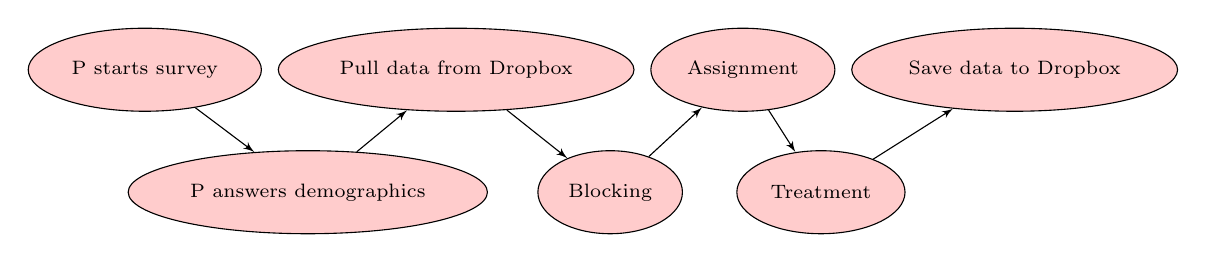
\begin{tikzpicture}
    \node [cloud]  (survey) {\scriptsize{P starts survey}};
    \node [cloud, below right=0.8cm and -0.6cm of survey] (dems) {\scriptsize{P answers demographics}};
    \node [cloud, right= 0.2cm of survey] (pulls) {\scriptsize{Pull data from Dropbox}};
    \node [cloud, below right=0.8cm and -0.3cm of pulls] (blocking) {\scriptsize{Blocking}};
    \node [cloud, right= 0.2cm of pulls] (assignment) {\scriptsize{Assignment}};
    \node [cloud, below right=0.8cm and -0.6cm of assignment] (treatment) {\scriptsize{Treatment}};
    \node [cloud, right= 0.2cm of assignment] (results) {\scriptsize{Save data to Dropbox}};
    \path [line] (survey) -- (dems);
    \path [line] (dems) -- (pulls);
    \path [line] (pulls) -- (blocking);
    \path [line] (blocking) -- (assignment);
    \path [line] (assignment) -- (treatment);
    \path [line] (treatment) -- (results);
\end{tikzpicture}
\caption{Online Survey Experiment Workflow} \label{online-workflow}
\end{figure}
A respondent clicks on the survey link and answers the demographic question. After she selects her level of education, \texttt{R} code in the background pulls previous respondents' covariate information from a Dropbox server. Based on this information and her chosen education level, the \texttt{R} code sequentially blocks and assigns her to a treatment group. The respondent then sees and answers the respective treatment question(s). Her responses are then saved on the same Dropbox server. This process is repeated for all incoming respondents. If the respondent is the first person to take the survey, i.e.~if there is no covariate information from previous respondents yet, the code randomly assigns her to one of the treatment groups. All subsequent respondents are then blocked and assigned as just described. To recruit respondents, the website was fed into Lucid's marketplace.

\hypertarget{app-ordblock-blockdiff}{%
\section{Blocking Differences}\label{app-ordblock-blockdiff}}

Figures \ref{ANBlock1} to \ref{ANBlock3} show the variable proportions or means, depending on the type of variable in question, after blocking the ANES data on education into three treatment groups. As outlined above, this is done twice, once based on the original ANES education categories, and once based on the newly estimated OP education categories.
\begin{figure}
\centering
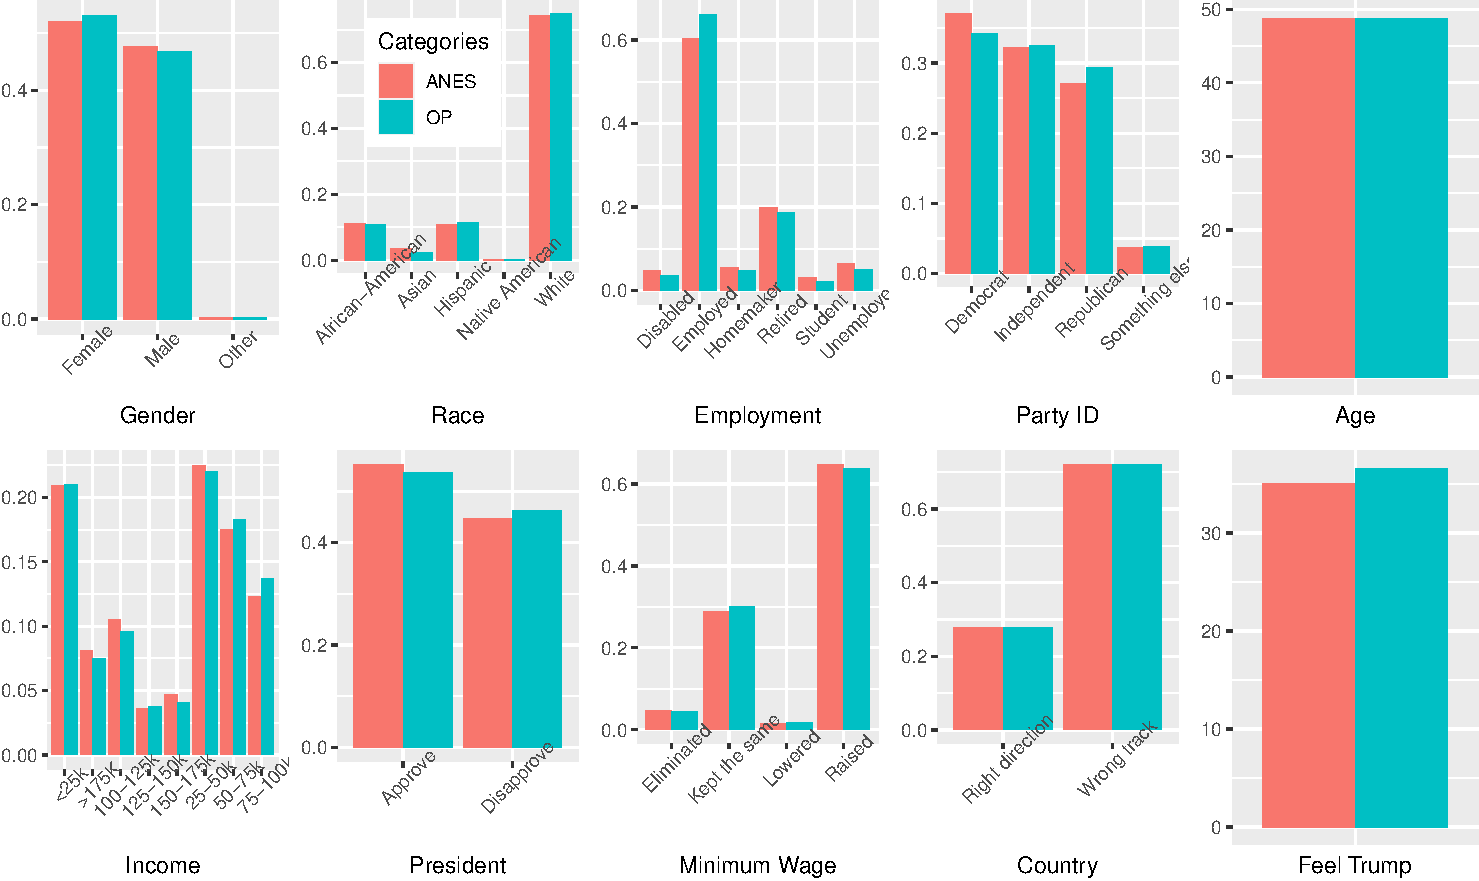
\includegraphics{dissertation_files/figure-latex/ANES-Blocked-Plot-1-1.pdf}
\caption{\label{fig:ANES-Blocked-Plot-1}Variable Proportions/Means After Blocking ANES Data on ANES and OP Education Categories, Treatment Group 1. \texttt{Age} and \texttt{Feel\ Trump} Show Means, All Others Show Proportions.\label{ANBlock1}}
\end{figure}
\begin{figure}
\centering
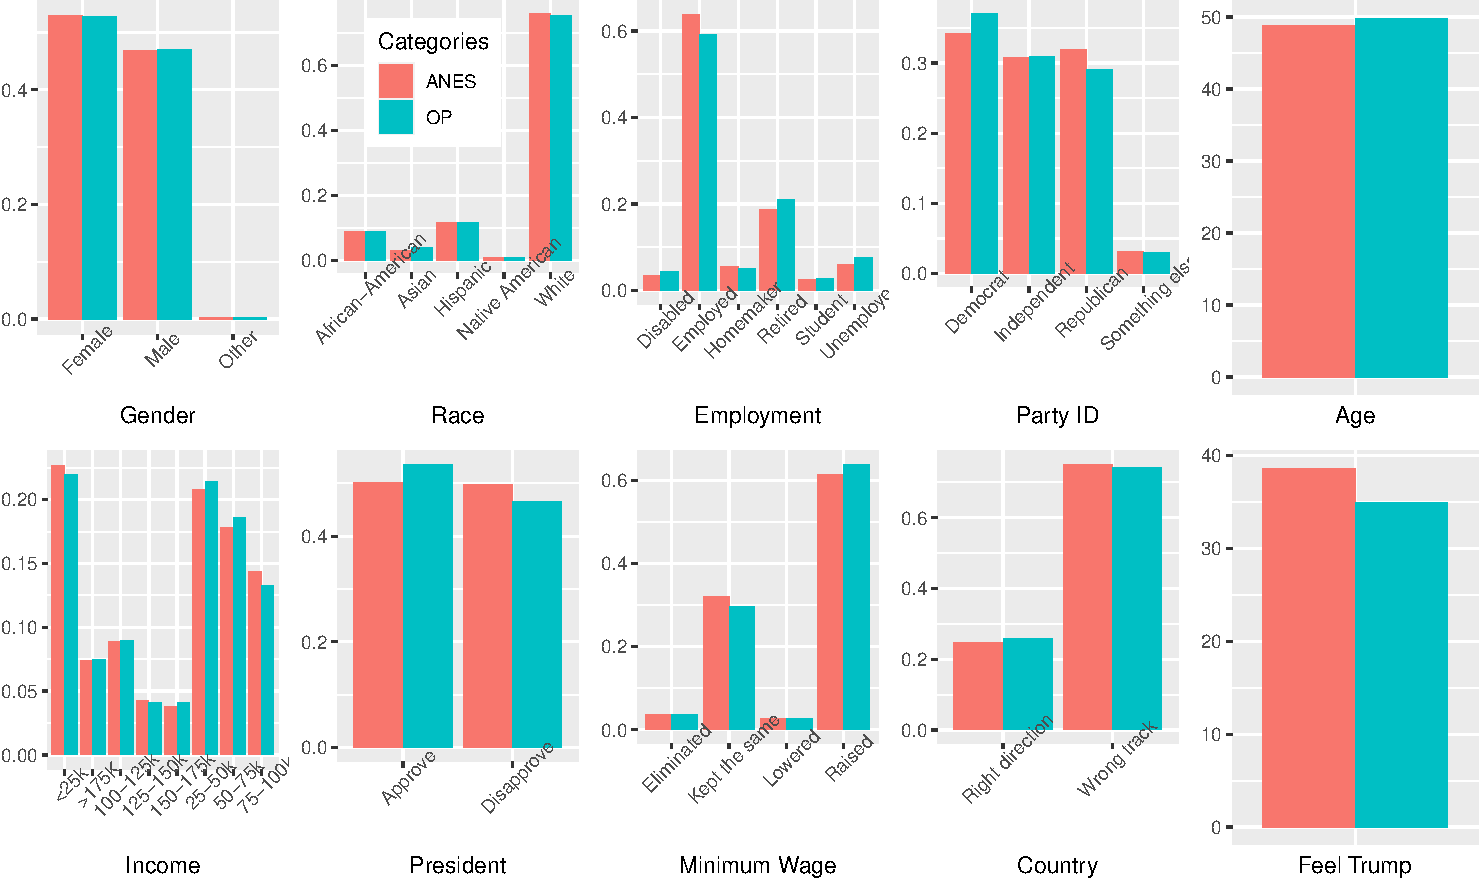
\includegraphics{dissertation_files/figure-latex/ANES-Blocked-Plot-2-1.pdf}
\caption{\label{fig:ANES-Blocked-Plot-2}Variable Proportions/Means After Blocking ANES Data on ANES and OP Education Categories, Treatment Group 2. \texttt{Age} and \texttt{Feel\ Trump} Show Means, All Others Show Proportions.\label{ANBlock2}}
\end{figure}
\begin{figure}
\centering
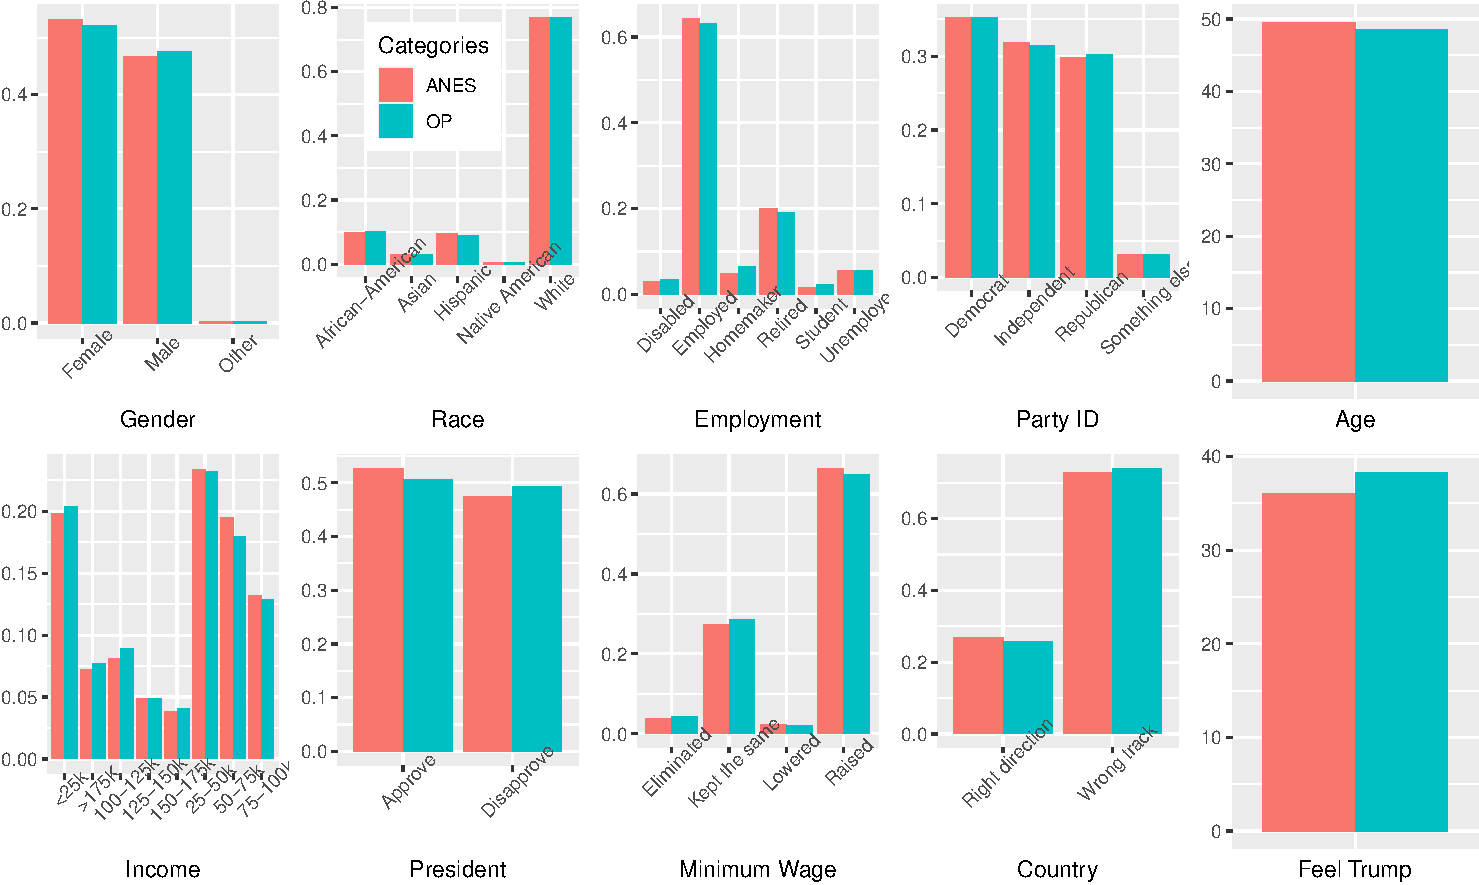
\includegraphics{dissertation_files/figure-latex/ANES-Blocked-Plot-3-1.pdf}
\caption{\label{fig:ANES-Blocked-Plot-3}Variable Proportions/Means After Blocking ANES Data on ANES and OP Education Categories, Treatment Group 3. \texttt{Age} and \texttt{Feel\ Trump} Show Means, All Others Show Proportions.\label{ANBlock3}}
\end{figure}
\hypertarget{app-ordmiss}{%
\chapter{MISSING DATA}\label{app-ordmiss}}

\hypertarget{app-ordmiss-allObs}{%
\section{Imputing Missing Data for All ANES and CCES Observations}\label{app-ordmiss-allObs}}

While using the full number of observations in the ANES data is possible, doing so for the CCES data provides great computational challenges. All 2,395 ANES observations can be used for 1,000 multiple imputation iterations. With over 42,000 observations, however, the number of iterations that are computationally feasible for the CCES data is reduced to 10. Anything above that maxes out the 120 GB RAM on the cloud container that was at my disposal, which results in termination of the code. Keeping these restrictions in mind, Tables \ref{mar.5var.all} and \ref{mnar.5var.all} show the results for MAR and MNAR for 5 variables with inserted missing data.
\begin{table}[!htbp] \centering    
 \caption{Accuracy of Multiple Imputation Methods. ANES and CCES Data, MAR, 5 Variables with NA, All Observations}  
 \label{mar.5var.all}
\begin{tabular}{ccr@{}lr@{}l} 
 \\[-1.8ex]\hline 
 \hline \\[-1.8ex]
 \multicolumn{1}{c}{Method} & \multicolumn{1}{c}{Variable} & \multicolumn{2}{c}{ANES} & \multicolumn{2}{c}{CCES} \\
 \hline \\[-1.8ex] 
 true & Democrat & 0.&3370 & 0.&4032 \\
 hd.ord & Democrat & --0.&0001 & + 0.&0006 \\
 hot.deck & Democrat & --0.&0002 & + 0.&0006 \\ 
 amelia & Democrat & + 0.&0000 & + 0.&0003 \\
 mice & Democrat & + 0.&0000 & + 0.&0003 \\
 na.omit & Democrat & --0.&0302 & --0.&0250 \\
 true & Male & 0.&4868 & 0.&4521 \\
 hd.ord & Male & --0.&0004 & --0.&0001 \\ 
 hot.deck & Male & --0.&0008 & --0.&0002 \\
 amelia & Male & + 0.&0001 & + 0.&0001 \\
 mice & Male & + 0.&0001 & + 0.&0001 \\
 na.omit & Male & --0.&0365 & --0.&0436 \\
 true & Interest & 2.&8806 & 3.&3301 \\
 hd.ord & Interest & --0.&0087 & --0.&0033 \\
 hot.deck & Interest & --0.&0135 & --0.&0046 \\
 amelia & Interest & + 0.&0001 & + 0.&0001 \\
 mice & Interest & + 0.&0000 & + 0.&0000 \\ 
 na.omit & Interest & --0.&0741 & --0.&0763 \\
 true & Income & 16.&6894 & 6.&5830 \\
 hd.ord & Income & --0.&0606 & --0.&0009 \\ 
 hot.deck & Income & --0.&1030 & --0.&0073 \\
 amelia & Income & + 0.&0009 & --0.&0021 \\
 mice & Income & --0.&0007 & --0.&0022 \\
 na.omit & Income & --0.&5574 & --0.&2592 \\
 true & Age & 50.&3745 & 52.&8639 \\
 hd.ord & Age & --0.&2355 & --0.&0221 \\ 
 hot.deck & Age & --0.&3698 & --0.&0790 \\ 
 amelia & Age & + 0.&0056 & --0.&0006 \\
 mice & Age & + 0.&0053 & --0.&0132 \\
 na.omit & Age & --1.&2785 & --1.&2190 \\
 \hline \\[-1.8ex] 
\multicolumn{2}{c}{Observations} & \multicolumn{2}{c}{2395} & \multicolumn{2}{c}{42205} \\ 
\multicolumn{2}{c}{Iterations} & \multicolumn{2}{c}{1000} & \multicolumn{2}{c}{10} \\ 
\hline \\[-1.8ex] 
 \end{tabular} 
 \end{table}
\begin{table}[!htbp] \centering   
 \caption{Accuracy of Multiple Imputation Methods. ANES and CCES Data, MNAR, 5 Variables with NA, All Observations}   
 \label{mnar.5var.all}  
\begin{tabular}{ccr@{}lr@{}l} 
 \\[-1.8ex]\hline 
 \hline \\[-1.8ex] 
 \multicolumn{1}{c}{Method} & \multicolumn{1}{c}{Variable} & \multicolumn{2}{c}{ANES} & \multicolumn{2}{c}{CCES} \\
 \hline \\[-1.8ex]  
 true & Democrat & 0.&3370 & 0.&4032 \\ 
 hd.ord & Democrat & --0.&0109 & --0.&0105 \\
 hot.deck & Democrat & --0.&0113 & --0.&0105 \\
 amelia & Democrat & --0.&0110 & --0.&0109 \\
 mice & Democrat & --0.&0103 & --0.&0106 \\
 na.omit & Democrat & --0.&0185 & --0.&0145 \\  
 true & Male & 0.&4868 & 0.&4521 \\ 
 hd.ord & Male & --0.&0138 & --0.&0129 \\ 
 hot.deck & Male & --0.&0136 & --0.&0131 \\ 
 amelia & Male & --0.&0134 & --0.&0132 \\
 mice & Male & --0.&0134 & --0.&0131 \\ 
 na.omit & Male & --0.&0196 & --0.&0244 \\ 
 true & Interest & 2.&8806 & 3.&3301 \\
 hd.ord & Interest & --0.&0257 & --0.&0171 \\
 hot.deck & Interest & --0.&0299 & --0.&0179 \\
 amelia & Interest & --0.&0178 & --0.&0147 \\
 mice & Interest & --0.&0179 & --0.&0148 \\
 na.omit & Interest & --0.&0407 & --0.&0418 \\
 true & Income & 16.&6894 & 6.&5830 \\
 hd.ord & Income & --0.&1874 & --0.&0691 \\ 
 hot.deck & Income & --0.&2287 & --0.&0696 \\
 amelia & Income & --0.&1292 & --0.&0637 \\
 mice & Income & --0.&1297 & --0.&0634 \\
 na.omit & Income & --0.&2729 & --0.&1375 \\
 true & Age & 50.&3745 & 52.&8639 \\ 
 hd.ord & Age & --0.&5240 & --0.&2331 \\
 hot.deck & Age & --0.&6609 & --0.&2764 \\
 amelia & Age & --0.&2533 & --0.&2342 \\
 mice & Age & --0.&2474 & --0.&2371 \\
 na.omit & Age & --0.&7188 & --0.&6476 \\
\hline \\[-1.8ex] 
\multicolumn{2}{c}{Observations} & \multicolumn{2}{c}{2395} & \multicolumn{2}{c}{42205} \\ 
\multicolumn{2}{c}{Iterations} & \multicolumn{2}{c}{1000} & \multicolumn{2}{c}{10} \\ 
\hline \\[-1.8ex] 
\end{tabular} 
\end{table}
\clearpage

\hypertarget{app-ordmiss-12var}{%
\section{Imputing 12 Variables with Missing Data}\label{app-ordmiss-12var}}

Table \ref{mar.12var} shows the results of imputing both data sets MAR for 12 amputed variables. The first five listed variables are the same as for the MAR analysis for five amputed variables in Table \ref{mar.5var}. The remaining variables were chosen based on availability in each data set. As much as possible, the same variables were selected across both data sets. \texttt{Black}, \texttt{Employed}, \texttt{Religious}, \texttt{Married}, \texttt{OwnHome}, \texttt{Rally}, \texttt{Donate}, \texttt{Gay}, \texttt{StudLoans}, \texttt{Hispanic}, \texttt{Official}, and \texttt{Student} are binary variables. \texttt{Black} indicates whether a respondent is of African-American origin, \texttt{Employed} whether she is currently employed, \texttt{Religious} whether she follows a religious belief, \texttt{Married} whether she is currently married, \texttt{OwnHome} whether she owns her home, \texttt{Rally} whether she has attended a political rally, \texttt{Donate} whether she has donated to a political candidate, \texttt{Gay} whether she identifies as homosexual, \texttt{StudLoans} whether she currently has student loans, \texttt{Hispanic} whether she is of Hispanic origin, \texttt{Official} whether she has contacted her political representative, and \texttt{Student} whether she currently is a student. \texttt{Media} is an ordinal variable and indicates how much she follows public affairs in the media (scaled from 1 to 5). \texttt{Participation} is an interval variable and shows the accumulative count of political activities she has participated in (scaled from 0 to 4).

\ssp

\footnotesize
\begin{longtable}{ccr@{}lr@{}l} 
 \caption{Accuracy of Multiple Imputation Methods. ANES and CCES Data, MAR, 12 Variables with NA}   
 \label{mar.12var} 
 \\[-1.8ex]\hline 
 \hline \\[-1.8ex] 
 \multicolumn{1}{c}{Method} & \multicolumn{1}{c}{Variable} & \multicolumn{2}{c}{ANES} & \multicolumn{2}{c}{CCES} \\
 \hline \\[-1.8ex] 
 true & Democrat & 0.&3420 & 0.&3770 \\ 
 hd.ord & Democrat & --0.&0005 & --0.&0003 \\
 hot.deck & Democrat & --0.&0005 & --0.&0004 \\
 amelia & Democrat & + 0.&0000 & + 0.&0000 \\
 mice & Democrat & + 0.&0000 & + 0.&0001 \\
 na.omit & Democrat & --0.&0191 & --0.&0172 \\
 true & Male & 0.&4890 & 0.&4830 \\ 
 hd.ord & Male & --0.&0004 & --0.&0002 \\
 hot.deck & Male & --0.&0001 & --0.&0003 \\  
 amelia & Male & + 0.&0001 & --0.&0001 \\
 mice & Male & + 0.&0000 & --0.&0002 \\
 na.omit & Male & --0.&0256 & --0.&0364 \\
 true & Interest & 2.&9340 & 3.&3290 \\
 hd.ord & Interest & --0.&0053 & --0.&0041 \\
 hot.deck & Interest & --0.&0077 & --0.&0067 \\
 amelia & Interest & + 0.&0001 & --0.&0001 \\
 mice & Interest & + 0.&0000 & --0.&0001 \\ 
 na.omit & Interest & --0.&0620 & --0.&0515 \\
 true & Income & 16.&6140 & 6.&4810 \\ 
 hd.ord & Income & --0.&0470 & --0.&0130 \\ 
 hot.deck & Income & --0.&0591 & --0.&0212 \\
 amelia & Income & --0.&0007 & --0.&0005 \\
 mice & Income & --0.&0013 & --0.&0003 \\ 
 na.omit & Income & --0.&6303 & --0.&2860 \\
 true & Age & 50.&0410 & 52.&8230 \\
 hd.ord & Age & --0.&1391 & --0.&0883 \\ 
 hot.deck & Age & --0.&1835 & --0.&1435 \\
 amelia & Age & + 0.&0056 & --0.&0015 \\ 
 mice & Age & + 0.&0048 & --0.&0050 \\ 
 na.omit & Age & --0.&8638 & --0.&5974 \\
 true & Black & 0.&0790 & 0.&0950 \\ 
 hd.ord & Black & + 0.&0000 & + 0.&0000 \\
 hot.deck & Black & + 0.&0000 & + 0.&0000 \\ 
 amelia & Black & + 0.&0000 & + 0.&0001 \\
 mice & Black & + 0.&0000 & + 0.&0001 \\ 
 na.omit & Black & --0.&0092 & --0.&0090 \\
 true & Employed & 0.&6610 & 0.&4370 \\ 
 hd.ord & Employed & + 0.&0006 & + 0.&0000 \\ 
 hot.deck & Employed & + 0.&0006 & + 0.&0001 \\
 amelia & Employed & + 0.&0000 & + 0.&0000 \\
 mice & Employed & + 0.&0000 & --0.&0001 \\
 na.omit & Employed & --0.&0087 & --0.&0301 \\
 true & Religious & 0.&6460 & 0.&6420 \\ 
 hd.ord & Religious & --0.&0006 & --0.&0003 \\ 
 hot.deck & Religious & --0.&0005 & --0.&0003 \\
 amelia & Religious & --0.&0001 & --0.&0001 \\
 mice & Religious & --0.&0001 & --0.&0002 \\ 
 na.omit & Religious & --0.&0166 & --0.&0234 \\ 
 true & Married & 0.&5290 & 0.&6310 \\
 hd.ord & Married & + 0.&0002 & --0.&0001 \\
 hot.deck & Married & + 0.&0002 & + 0.&0001 \\
 amelia & Married & --0.&0001 & --0.&0002 \\
 mice & Married & --0.&0001 & --0.&0002 \\ 
 na.omit & Married & --0.&0384 & --0.&0326 \\ 
 true & OwnHome & 0.&6820 & 0.&7010 \\
 hd.ord & OwnHome & --0.&0001 & --0.&0002 \\ 
 hot.deck & OwnHome & + 0.&0000 & + 0.&0000 \\ 
 amelia & OwnHome & + 0.&0001 & + 0.&0000 \\ 
 mice & OwnHome & --0.&0001 & --0.&0001 \\
 na.omit & OwnHome & --0.&0334 & --0.&0304 \\
 true & Rally & 0.&0830 & --- \\
 hd.ord & Rally & --0.&0001 & --- \\ 
 hot.deck & Rally & --0.&0002 & --- \\ 
 amelia & Rally & + 0.&0001 & --- \\ 
 mice & Rally & + 0.&0001 & --- \\ 
 na.omit & Rally & --0.&0191 & --- \\ 
 true & Donate & 0.&1390 & --- \\ 
 hd.ord & Donate & --0.&0002 & --- \\ 
 hot.deck & Donate & --0.&0005 & --- \\
 amelia & Donate & + 0.&0000 & --- \\ 
 mice & Donate & + 0.&0001 & --- \\ 
 na.omit & Donate & --0.&0320 & --- \\ 
 true & Gay & \multicolumn{2}{l}{---} & 0.&0420 \\ 
 hd.ord & Gay & \multicolumn{2}{l}{---}  & + 0.&0001 \\
 hot.deck & Gay & \multicolumn{2}{l}{---} & + 0.&0000 \\ 
 amelia & Gay & \multicolumn{2}{l}{---} & + 0.&0000 \\
 mice & Gay & \multicolumn{2}{l}{---} & + 0.&0000 \\
 na.omit & Gay & \multicolumn{2}{l}{---} &  --0.&0112 \\
 true & StudLoans & \multicolumn{2}{l}{---} & 0.&1910 \\
 hd.ord & StudLoans & \multicolumn{2}{l}{---} & + 0.&0003 \\
 hot.deck & StudLoans & \multicolumn{2}{l}{---} & + 0.&0002 \\
 amelia & StudLoans & \multicolumn{2}{l}{---} & + 0.&0000 \\
 mice & StudLoans & \multicolumn{2}{l}{---} & --0.&0001 \\
 na.omit & StudLoans & \multicolumn{2}{l}{---} & --0.&0117 \\ 
 \hline \\[-1.8ex]
 \end{longtable}
\dsp

\normalsize

The results are consistent with those presented in Table \ref{mar.5var}. For the binary variables, \texttt{amelia} and \texttt{mice} again perform best with results actually matching the true variable values, though \texttt{hd.ord} arguably shows closer results than in Table \ref{mar.5var} with a maximum difference to a true value of +0.0006 (ANES \texttt{Employed}). For the ordinal variable, \texttt{hd.ord} continues to perform worst across both data sets. \texttt{mice} and \texttt{amelia} again show the best results. Note, however, that \texttt{hd.ord} is less worse in terms of performance differences when compared to the MAR analysis of five imputed variables. The maximum difference to the true \texttt{Interest} value is --0.0053 (ANES) for 12 variables but --0.0130 (ANES) for five variables. This is possibly explained by a thinner spread of missing values across a higher number of variables, resulting in a lower number of NAs in each amputed variable.

The results for the interval variables follow the same pattern: \texttt{hd.ord} displays the worst results for both data sets. The difference to \texttt{hot.deck} is still present though less pronounced than in the MAR analysis of five imputed variables. \texttt{mice} overall performs better than \texttt{amelia} for \texttt{Income} and \texttt{Age}, with the exceptions of ANES \texttt{Income} (--0.0007 vs.~--0.0013) and CCES \texttt{Age} (--0.0015 vs.~--0.0050).

Table \ref{mnar.12var} shows the results of imputing both data sets MNAR for 12 amputed variables. The results are consistent with those obtained for five amputed variables MNAR. \texttt{amelia} and \texttt{mice} perform better than \texttt{hd.ord} for the binary variables overall, but often not by much. Occasionally, \texttt{hd.ord} eclipses them (--0.0055 vs.~--0.0055 \texttt{mice} and \texttt{amelia} ANES \texttt{Male}). \texttt{na.omit} once more performs close to the other methods.

\ssp

\footnotesize
\begin{longtable}{ccr@{}lr@{}l} 
 \caption{Accuracy of Multiple Imputation Methods. ANES and CCES Data, MNAR, 12 Variables with NA}  
 \label{mnar.12var} 
 \\[-1.8ex]\hline 
 \hline \\[-1.8ex]
 \multicolumn{1}{c}{Method} & \multicolumn{1}{c}{Variable} & \multicolumn{2}{c}{ANES} & \multicolumn{2}{c}{CCES} \\
 \hline \\[-1.8ex] 
 true & Democrat & 0.&3420 & 0.&3770 \\
 hd.ord & Democrat & --0.&0049 & --0.&0046 \\
 hot.deck & Democrat & --0.&0049 & --0.&0049 \\
 amelia & Democrat & --0.&0043 & --0.&0045 \\
 mice & Democrat & --0.&0040 & --0.&0044 \\ 
 na.omit & Democrat & --0.&0092 & --0.&0081 \\
 true & Male & 0.&4890 & 0.&4830 \\ 
 hd.ord & Male & --0.&0055 & --0.&0049 \\ 
 hot.deck & Male & --0.&0053 & --0.&0051 \\ 
 amelia & Male & --0.&0055 & --0.&0050 \\
 mice & Male & --0.&0055 & --0.&0049 \\
 na.omit & Male & --0.&0093 & --0.&0119 \\ 
 true & Interest & 2.&9340 & 3.&3290 \\
 hd.ord & Interest & --0.&0113 & --0.&0090 \\ 
 hot.deck & Interest & --0.&0134 & --0.&0113 \\
 amelia & Interest & --0.&0068 & --0.&0061 \\
 mice & Interest & --0.&0068 & --0.&0061 \\
 na.omit & Interest & --0.&0236 & --0.&0161 \\ 
 true & Income & 16.&6140 & 6.&4810 \\ 
 hd.ord & Income & --0.&0899 & --0.&0350 \\ 
 hot.deck & Income & --0.&1046 & --0.&0421 \\
 amelia & Income & --0.&0495 & --0.&0223 \\
 mice & Income & --0.&0503 & --0.&0218 \\ 
 na.omit & Income & --0.&2088 & --0.&0970 \\
 true & Age & 50.&0410 & 52.&8230 \\ 
 hd.ord & Age & --0.&2571 & --0.&1732 \\ 
 hot.deck & Age & --0.&3081 & --0.&2251 \\
 amelia & Age & --0.&1100 & --0.&1014 \\ 
 mice & Age & --0.&1047 & --0.&0986 \\ 
 na.omit & Age & --0.&3397 & --0.&1367 \\
 true & Black & 0.&0790 & 0.&0950 \\
 hd.ord & Black & --0.&0035 & --0.&0038 \\
 hot.deck & Black & --0.&0037 & --0.&0038 \\ 
 amelia & Black & --0.&0037 & --0.&0040 \\ 
 mice & Black & --0.&0034 & --0.&0038 \\
 na.omit & Black & --0.&0045 & --0.&0052 \\
 true & Employed & 0.&6610 & 0.&4370 \\
 hd.ord & Employed & --0.&0034 & --0.&0053 \\
 hot.deck & Employed & --0.&0033 & --0.&0053 \\
 amelia & Employed & --0.&0031 & --0.&0040 \\
 mice & Employed & --0.&0031 & --0.&0040 \\ 
 na.omit & Employed & --0.&0014 & --0.&0111 \\ 
 true & Religious & 0.&6460 & 0.&6420 \\ 
 hd.ord & Religious & --0.&0045 & --0.&0039 \\
 hot.deck & Religious & --0.&0043 & --0.&0038 \\
 amelia & Religious & --0.&0040 & --0.&0040 \\
 mice & Religious & --0.&0040 & --0.&0040 \\ 
 na.omit & Religious & --0.&0049 & --0.&0073 \\ 
 true & Married & 0.&5290 & 0.&6310 \\ 
 hd.ord & Married & --0.&0041 & --0.&0038 \\
 hot.deck & Married & --0.&0040 & --0.&0037 \\ 
 amelia & Married & --0.&0042 & --0.&0037 \\ 
 mice & Married & --0.&0042 & --0.&0037 \\ 
 na.omit & Married & --0.&0122 & --0.&0096 \\ 
 true & OwnHome & 0.&6820 & 0.&7010 \\ 
 hd.ord & OwnHome & --0.&0030 & --0.&0030 \\ 
 hot.deck & OwnHome & --0.&0028 & --0.&0027 \\
 amelia & OwnHome & --0.&0027 & --0.&0030 \\ 
 mice & OwnHome & --0.&0027 & --0.&0030 \\ 
 na.omit & OwnHome & --0.&0111 & --0.&0090 \\
 true & Rally & 0.&0830 & --- \\ 
 hd.ord & Rally & --0.&0043 & --- \\ 
 hot.deck & Rally & --0.&0042 & --- \\ 
 amelia & Rally & --0.&0040 & --- \\ 
 mice & Rally & --0.&0039 & --- \\ 
 na.omit & Rally & --0.&0077 & --- \\  
 true & Donate & 0.&1390 & --- \\ 
 hd.ord & Donate & --0.&0051 & --- \\ 
 hot.deck & Donate & --0.&0054 & --- \\ 
 amelia & Donate & --0.&0049 & --- \\ 
 mice & Donate & --0.&0048 & --- \\ 
 na.omit & Donate & --0.&0122 & --- \\ 
 true & Gay & \multicolumn{2}{l}{---} & 0.&0420 \\ 
 hd.ord & Gay & \multicolumn{2}{l}{---} & --0.&0024 \\ 
 hot.deck & Gay & \multicolumn{2}{l}{---} & --0.&0025 \\ 
 amelia & Gay & \multicolumn{2}{l}{---} & --0.&0026 \\
 mice & Gay & \multicolumn{2}{l}{---} & --0.&0024 \\ 
 na.omit & Gay & \multicolumn{2}{l}{---} & --0.&0035 \\ 
 true & StudLoans & \multicolumn{2}{l}{---} & 0.&1910 \\
 hd.ord & StudLoans & \multicolumn{2}{l}{---} & --0.&0058 \\
 hot.deck & StudLoans & \multicolumn{2}{l}{---} & --0.&0058 \\ 
 amelia & StudLoans & \multicolumn{2}{l}{---} & --0.&0051 \\ 
 mice & StudLoans & \multicolumn{2}{l}{---} & --0.&0050 \\ 
 na.omit & StudLoans & \multicolumn{2}{l}{---} & --0.&0070 \\ 
 \hline \\[-1.8ex]
 \end{longtable}
\dsp

\normalsize

For the ordinal variable, \texttt{hd.ord} shows the worst performance across both data sets. \texttt{mice} and \texttt{amelia} perform far better and display virtually identical results. \texttt{na.omit} does not perform as well as in the corresponding MAR analysis. \texttt{mice} and \texttt{amelia}'s superior performance is also visible in the results for the ordinal variables. \texttt{na.omit} performs better than \texttt{hot.deck} and \texttt{hd.ord} for CCES \texttt{Age} (--0.1367 vs.~--0.2251 and --0.1732).

\hypertarget{app-ordmiss-mult-11var}{%
\section{Imputing 11 Variables with Missing Data for Two Ordinal Variables}\label{app-ordmiss-mult-11var}}

Table \ref{mult.mar.11var} shows the results of imputing both data sets with two \texttt{polr}-treated variables MAR for 11 amputed variables. A similar picture for Table \ref{mult.mar.4var} emerges for the binary variables, with \texttt{amelia} and \texttt{mice} once more displaying the best results, though \texttt{hd.ord} appears to perform somewhat closer here. Consistent with the deterioration of \texttt{hd.ord} results from Table \ref{mar.5var} to Table \ref{mult.mar.4var}, \texttt{hd.ord} again consistently performs slightly worse when compared to the MAR analysis with 12 amputed variables and only \texttt{Education} treated by \texttt{polr}: --0.0002, --0.0004 vs.~--0.0005, --0.0003 for \texttt{Democrat} and --0.0002, --0.0005 vs.~--0.0004, --0.0002 for \texttt{Male}.

\ssp

\footnotesize
\begin{longtable}{ccr@{}lr@{}l} 
 \caption{Accuracy of Multiple Imputation Methods. ANES and CCES Data, 2 Ordinal Variables (Education, Interest), MAR, 11 Variables with NA} 
 \label{mult.mar.11var}  
 \\[-1.8ex]\hline 
 \hline \\[-1.8ex]
 \multicolumn{1}{c}{Method} & \multicolumn{1}{c}{Variable} & \multicolumn{2}{c}{ANES} & \multicolumn{2}{c}{CCES} \\
 \hline \\[-1.8ex]
 true & Democrat & 0.&3420 & 0.&3770 \\ 
 hd.ord & Democrat & --0.&0002 & --0.&0004 \\ 
 hot.deck & Democrat & --0.&0005 & --0.&0005 \\ 
 amelia & Democrat & + 0.&0000 & --0.&0001 \\ 
 mice & Democrat & + 0.&0000 & + 0.&0000 \\ 
 na.omit & Democrat & --0.&0200 & --0.&0213 \\
 true & Male & 0.&4890 & 0.&4830 \\ 
 hd.ord & Male & --0.&0002 & --0.&0005 \\
 hot.deck & Male & --0.&0001 & --0.&0004 \\
 amelia & Male & + 0.&0000 & --0.&0001 \\
 mice & Male & + 0.&0000 & --0.&0001 \\ 
 na.omit & Male & --0.&0254 & --0.&0350 \\ 
 true & Income & 16.&6140 & 6.&4810 \\ 
 hd.ord & Income & --0.&0346 & --0.&0114 \\
 hot.deck & Income & --0.&0657 & --0.&0241 \\ 
 amelia & Income & --0.&0018 & --0.&0007 \\
 mice & Income & --0.&0027 & --0.&0005 \\
 na.omit & Income & --0.&6432 & --0.&2888 \\
 true & Age & 50.&0410 & 52.&8230 \\ 
 hd.ord & Age & --0.&0887 & --0.&0704 \\
 hot.deck & Age & --0.&1951 & --0.&1532 \\
 amelia & Age & + 0.&0010 & --0.&0021 \\
 mice & Age & --0.&0016 & --0.&0055 \\ 
 na.omit & Age & --0.&8025 & --0.&4330 \\
 true & Black & 0.&0790 & 0.&0950 \\
 hd.ord & Black & + 0.&0001 & --0.&0001 \\
 hot.deck & Black & + 0.&0000 & --0.&0001 \\
 amelia & Black & + 0.&0000 & + 0.&0001 \\ 
 mice & Black & + 0.&0001 & + 0.&0001 \\ 
 na.omit & Black & --0.&0103 & --0.&0122 \\ 
 true & Employed & 0.&6610 & 0.&4370 \\
 hd.ord & Employed & + 0.&0007 & + 0.&0003 \\
 hot.deck & Employed & + 0.&0008 & + 0.&0001 \\ 
 amelia & Employed & + 0.&0001 & + 0.&0000 \\
 mice & Employed & + 0.&0001 & --0.&0001 \\
 na.omit & Employed & --0.&0109 & --0.&0328 \\
 true & Religious & 0.&6460 & 0.&6420 \\ 
 hd.ord & Religious & --0.&0001 & --0.&0002 \\ 
 hot.deck & Religious & --0.&0005 & --0.&0003 \\ 
 amelia & Religious & + 0.&0000 & --0.&0001 \\
 mice & Religious & + 0.&0000 & --0.&0002 \\
 na.omit & Religious & --0.&0174 & --0.&0241 \\ 
 true & Married & 0.&5290 & 0.&6310 \\ 
 hd.ord & Married & --0.&0001 & --0.&0002 \\ 
 hot.deck & Married & + 0.&0003 & + 0.&0001 \\ 
 amelia & Married & --0.&0001 & --0.&0002 \\ 
 mice & Married & --0.&0001 & --0.&0002 \\ 
 na.omit & Married & --0.&0390 & --0.&0324 \\ 
 true & OwnHome & 0.&6820 & 0.&7010 \\ 
 hd.ord & OwnHome & --0.&0005 & --0.&0001 \\
 hot.deck & OwnHome & --0.&0001 & + 0.&0002 \\ 
 amelia & OwnHome & + 0.&0000 & + 0.&0001 \\
 mice & OwnHome & --0.&0001 & + 0.&0000 \\
 na.omit & OwnHome & --0.&0341 & --0.&0295 \\
 true & Rally & 0.&0830 & --- \\ 
 hd.ord & Rally & + 0.&0000 & --- \\ 
 hot.deck & Rally & --0.&0002 & --- \\
 amelia & Rally & + 0.&0001 & --- \\ 
 mice & Rally & + 0.&0002 & --- \\
 na.omit & Rally & --0.&0186 & --- \\ 
 true & Donate & 0.&1390 & --- \\ 
 hd.ord & Donate & --0.&0003 & --- \\ 
 hot.deck & Donate & --0.&0007 & --- \\
 amelia & Donate & --0.&0001 & --- \\
 mice & Donate & + 0.&0000 & --- \\ 
 na.omit & Donate & --0.&0310 & --- \\ 
 true & Gay & \multicolumn{2}{l}{---} & 0.&0420 \\ 
 hd.ord & Gay & \multicolumn{2}{l}{---} & + 0.&0001 \\ 
 hot.deck & Gay & \multicolumn{2}{l}{---} & + 0.&0000 \\ 
 amelia & Gay & \multicolumn{2}{l}{---} & + 0.&0000 \\ 
 mice & Gay & \multicolumn{2}{l}{---} & + 0.&0001 \\
 na.omit & Gay & \multicolumn{2}{l}{---} & --0.&0113 \\ 
 true & StudLoans & \multicolumn{2}{l}{---} & 0.&1910 \\
 hd.ord & StudLoans & \multicolumn{2}{l}{---} & + 0.&0001 \\ 
 hot.deck & StudLoans & \multicolumn{2}{l}{---} & + 0.&0001 \\
 amelia & StudLoans & \multicolumn{2}{l}{---} & --0.&0001 \\ 
 mice & StudLoans & \multicolumn{2}{l}{---} & --0.&0001 \\ 
 na.omit & StudLoans & \multicolumn{2}{l}{---} & --0.&0146 \\
 \hline \\[-1.8ex] 
 \end{longtable}
\dsp

\normalsize

The same can be observed for the interval variables, with \texttt{hd.ord} again claiming last place across both data sets. The difference to \texttt{hot.deck} is still there but less pronounced than in Table \ref{mult.mar.4var}. \texttt{amelia} does best for \texttt{Age} while \texttt{mice} performs better for \texttt{Income}, with the exception of the ANES (--0.0027 \texttt{mice} vs.~--0.0018 \texttt{amelia}). As for the binary variables, \texttt{hd.ord} also consistently performs slightly worse when compared to the MAR analysis with 12 amputed variables and only \texttt{Education} treated by \texttt{polr}: --0.0346, --0.0114 vs.~--0.0470, --0.0130 for \texttt{Income} and --0.0887, --0.0704 vs.~--0.1391, --0.0883 for \texttt{Age}.

Table \ref{mult.mnar.11var} shows the results of imputing both data sets with two \texttt{polr}-treated variables MNAR for 11 amputed variables. For the binary variables, \texttt{amelia} and \texttt{mice} perform better, but often not by much. Occasionally, \texttt{hd.ord} eclipses them (--0.0061 \texttt{hd.ord} vs.~--0.0060 \texttt{mice} ANES \texttt{Male}). As was the case in the comparison between the MNAR analysis with four amputed variables and the MNAR analysis with five amputed variables, \texttt{hd.ord} consistently demonstrates slightly worse results in the switch from 12 (Table \ref{mnar.12var}) to 11 and one to two \texttt{polr}-treated variables: --0.0050, --0.0053 vs.~--0.0049, --0.0046 for \texttt{Democrat} and --0.0061, --0.0058 vs.~--0.0055, --0.0049 for \texttt{Male}.

\ssp

\footnotesize
\begin{longtable}{ccr@{}lr@{}l} 
 \caption{Accuracy of Multiple Imputation Methods. ANES and CCES Data, 2 Ordinal Variables (Education, Interest), MNAR, 11 Variables with NA}   
 \label{mult.mnar.11var}
 \\[-1.8ex]\hline  
 \hline \\[-1.8ex] 
 \multicolumn{1}{c}{Method} & \multicolumn{1}{c}{Variable} & \multicolumn{2}{c}{ANES} & \multicolumn{2}{c}{CCES} \\
 \hline \\[-1.8ex] 
 true & Democrat & 0.&3420 & 0.&3770 \\ 
 hd.ord & Democrat & --0.&0050 & --0.&0053 \\ 
 hot.deck & Democrat & --0.&0053 & --0.&0053 \\
 amelia & Democrat & --0.&0047 & --0.&0049 \\
 mice & Democrat & --0.&0044 & --0.&0048 \\ 
 na.omit & Democrat & --0.&0097 & --0.&0097 \\
 true & Male & 0.&4890 & 0.&4830 \\ 
 hd.ord & Male & --0.&0061 & --0.&0058 \\ 
 hot.deck & Male & --0.&0057 & --0.&0056 \\ 
 amelia & Male & --0.&0060 & --0.&0054 \\ 
 mice & Male & --0.&0060 & --0.&0054 \\ 
 na.omit & Male & --0.&0088 & --0.&0116 \\ 
 true & Income & 16.&6140 & 6.&4810 \\
 hd.ord & Income & --0.&0841 & --0.&0349 \\
 hot.deck & Income & --0.&1142 & --0.&0473 \\
 amelia & Income & --0.&0540 & --0.&0250 \\ 
 mice & Income & --0.&0549 & --0.&0249 \\ 
 na.omit & Income & --0.&2112 & --0.&0982 \\
 true & Age & 50.&0410 & 52.&8230 \\ 
 hd.ord & Age & --0.&2124 & --0.&1607 \\ 
 hot.deck & Age & --0.&3329 & --0.&2424 \\ 
 amelia & Age & --0.&1194 & --0.&1135 \\ 
 mice & Age & --0.&1141 & --0.&1102 \\ 
 na.omit & Age & --0.&2978 & --0.&0974 \\ 
 true & Black & 0.&0790 & 0.&0950 \\ 
 hd.ord & Black & --0.&0036 & --0.&0045 \\
 hot.deck & Black & --0.&0040 & --0.&0042 \\
 amelia & Black & --0.&0041 & --0.&0044 \\ 
 mice & Black & --0.&0037 & --0.&0041 \\ 
 na.omit & Black & --0.&0050 & --0.&0066 \\ 
 true & Employed & 0.&6610 & 0.&4370 \\ 
 hd.ord & Employed & --0.&0042 & --0.&0057 \\ 
 hot.deck & Employed & --0.&0036 & --0.&0058 \\ 
 amelia & Employed & --0.&0034 & --0.&0045 \\ 
 mice & Employed & --0.&0033 & --0.&0044 \\ 
 na.omit & Employed & --0.&0022 & --0.&0122 \\ 
 true & Religious & 0.&6460 & 0.&6420 \\
 hd.ord & Religious & --0.&0045 & --0.&0044 \\
 hot.deck & Religious & --0.&0047 & --0.&0042 \\
 amelia & Religious & --0.&0043 & --0.&0045 \\ 
 mice & Religious & --0.&0043 & --0.&0045 \\ 
 na.omit & Religious & --0.&0055 & --0.&0077 \\ 
 true & Married & 0.&5290 & 0.&6310 \\ 
 hd.ord & Married & --0.&0047 & --0.&0043 \\ 
 hot.deck & Married & --0.&0042 & --0.&0040 \\
 amelia & Married & --0.&0046 & --0.&0039 \\ 
 mice & Married & --0.&0045 & --0.&0039 \\ 
 na.omit & Married & --0.&0120 & --0.&0095 \\
 true & OwnHome & 0.&6820 & 0.&7010 \\
 hd.ord & OwnHome & --0.&0037 & --0.&0035 \\ 
 hot.deck & OwnHome & --0.&0030 & --0.&0030 \\
 amelia & OwnHome & --0.&0031 & --0.&0033 \\
 mice & OwnHome & --0.&0030 & --0.&0033 \\ 
 na.omit & OwnHome & --0.&0112 & --0.&0088 \\ 
 true & Rally & 0.&0830 & --- \\ 
 hd.ord & Rally & --0.&0047 & --- \\ 
 hot.deck & Rally & --0.&0047 & --- \\ 
 amelia & Rally & --0.&0045 & --- \\
 mice & Rally & --0.&0044 & --- \\
 na.omit & Rally & --0.&0080 & --- \\
 true & Donate & 0.&1390 & --- \\
 hd.ord & Donate & --0.&0057 & --- \\ 
 hot.deck & Donate & --0.&0060 & --- \\ 
 amelia & Donate & --0.&0054 & --- \\  
 mice & Donate & --0.&0053 & --- \\ 
 na.omit & Donate & --0.&0122 & --- \\ 
 true & Gay & \multicolumn{2}{l}{---} & 0.&0420 \\ 
 hd.ord & Gay & \multicolumn{2}{l}{---} & --0.&0027 \\
 hot.deck & Gay & \multicolumn{2}{l}{---} & --0.&0026 \\ 
 amelia & Gay & \multicolumn{2}{l}{---} & --0.&0028 \\ 
 mice & Gay & \multicolumn{2}{l}{---} & --0.&0027 \\ 
 na.omit & Gay & \multicolumn{2}{l}{---} & --0.&0037 \\
 true & StudLoans & \multicolumn{2}{l}{---} & 0.&1910 \\
 hd.ord & StudLoans & \multicolumn{2}{l}{---} & --0.&0067 \\
 hot.deck & StudLoans & \multicolumn{2}{l}{---} & --0.&0064 \\
 amelia & StudLoans & \multicolumn{2}{l}{---} & --0.&0057 \\
 mice & StudLoans & \multicolumn{2}{l}{---} & --0.&0056 \\ 
 na.omit & StudLoans & \multicolumn{2}{l}{---} & --0.&0082 \\
 \hline \\[-1.8ex] 
 \end{longtable}
\dsp

\normalsize

Finally, the results for the interval variables confirm previous results, with \texttt{amelia} and \texttt{mice} demonstrating the best performance. In addition, note that \texttt{na.omit} delivers better results than \texttt{hd.ord} for \texttt{Age} for both data sets and represents the best method for CCES \texttt{Age}. Similar to the MNAR results for four variables, the performance of \texttt{hd.ord} in the MNAR analysis of 11 variables deteriorates in the switch from one to two ordinal variables: --0.0841, --0.0349 vs.~--0.0899, --0.0350 for \texttt{Income} and --0.2124, --0.1607 vs.~--0.2571, --0.1732 for \texttt{Age}.

\hypertarget{app-ordmiss-speed-12var}{%
\section{Speed for 12 Imputed Variables}\label{app-ordmiss-speed-12var}}

The difference between the methods is somewhat less pronounced for 12 variables with missing data when compared to 5 variables. This could possibly be explained by the thinner spread of missing values across a higher number of variables. The substantive conclusions nonetheless remain the same.
\begin{table}[!htbp] \centering 
  \caption{Runtimes of Multiple Imputation Methods (in Minutes). ANES and CCES Data, MAR, 12 Variables with NA} 
  \label{runtimes12var} 
\begin{tabular}{@{\extracolsep{5pt}} D{.}{.}{-3} D{.}{.}{-3} D{.}{.}{-3} } 
\\[-1.8ex]\hline 
\hline \\[-1.8ex] 
\multicolumn{1}{c}{} & \multicolumn{1}{c}{ANES} & \multicolumn{1}{c}{CCES} \\ 
\hline \\[-1.8ex] 
\multicolumn{1}{c}{hd.ord} & 2.614 & 2.679 \\ 
\multicolumn{1}{c}{hot.deck} & 2.640 & 2.690 \\ 
\multicolumn{1}{c}{amelia} & 9.038 & 10.345 \\ 
\multicolumn{1}{c}{mice} & 104.143 & 113.390 \\ 
\hline \\[-1.8ex] 
\end{tabular} 
\end{table}
\hypertarget{app-framing}{%
\chapter{FRAMING}\label{app-framing}}

\hypertarget{app-framing-questionnaire}{%
\section{Framing Questionnaire}\label{app-framing-questionnaire}}
\begin{figure}[hbt]
  \centering

\includegraphics{data/framing/appendix/questionnaire/questionnaire01.jpg}
  \caption{Questionnaire}
  \label{framing-questionnaire}
\end{figure}
\begin{figure}[hbt]
  \centering
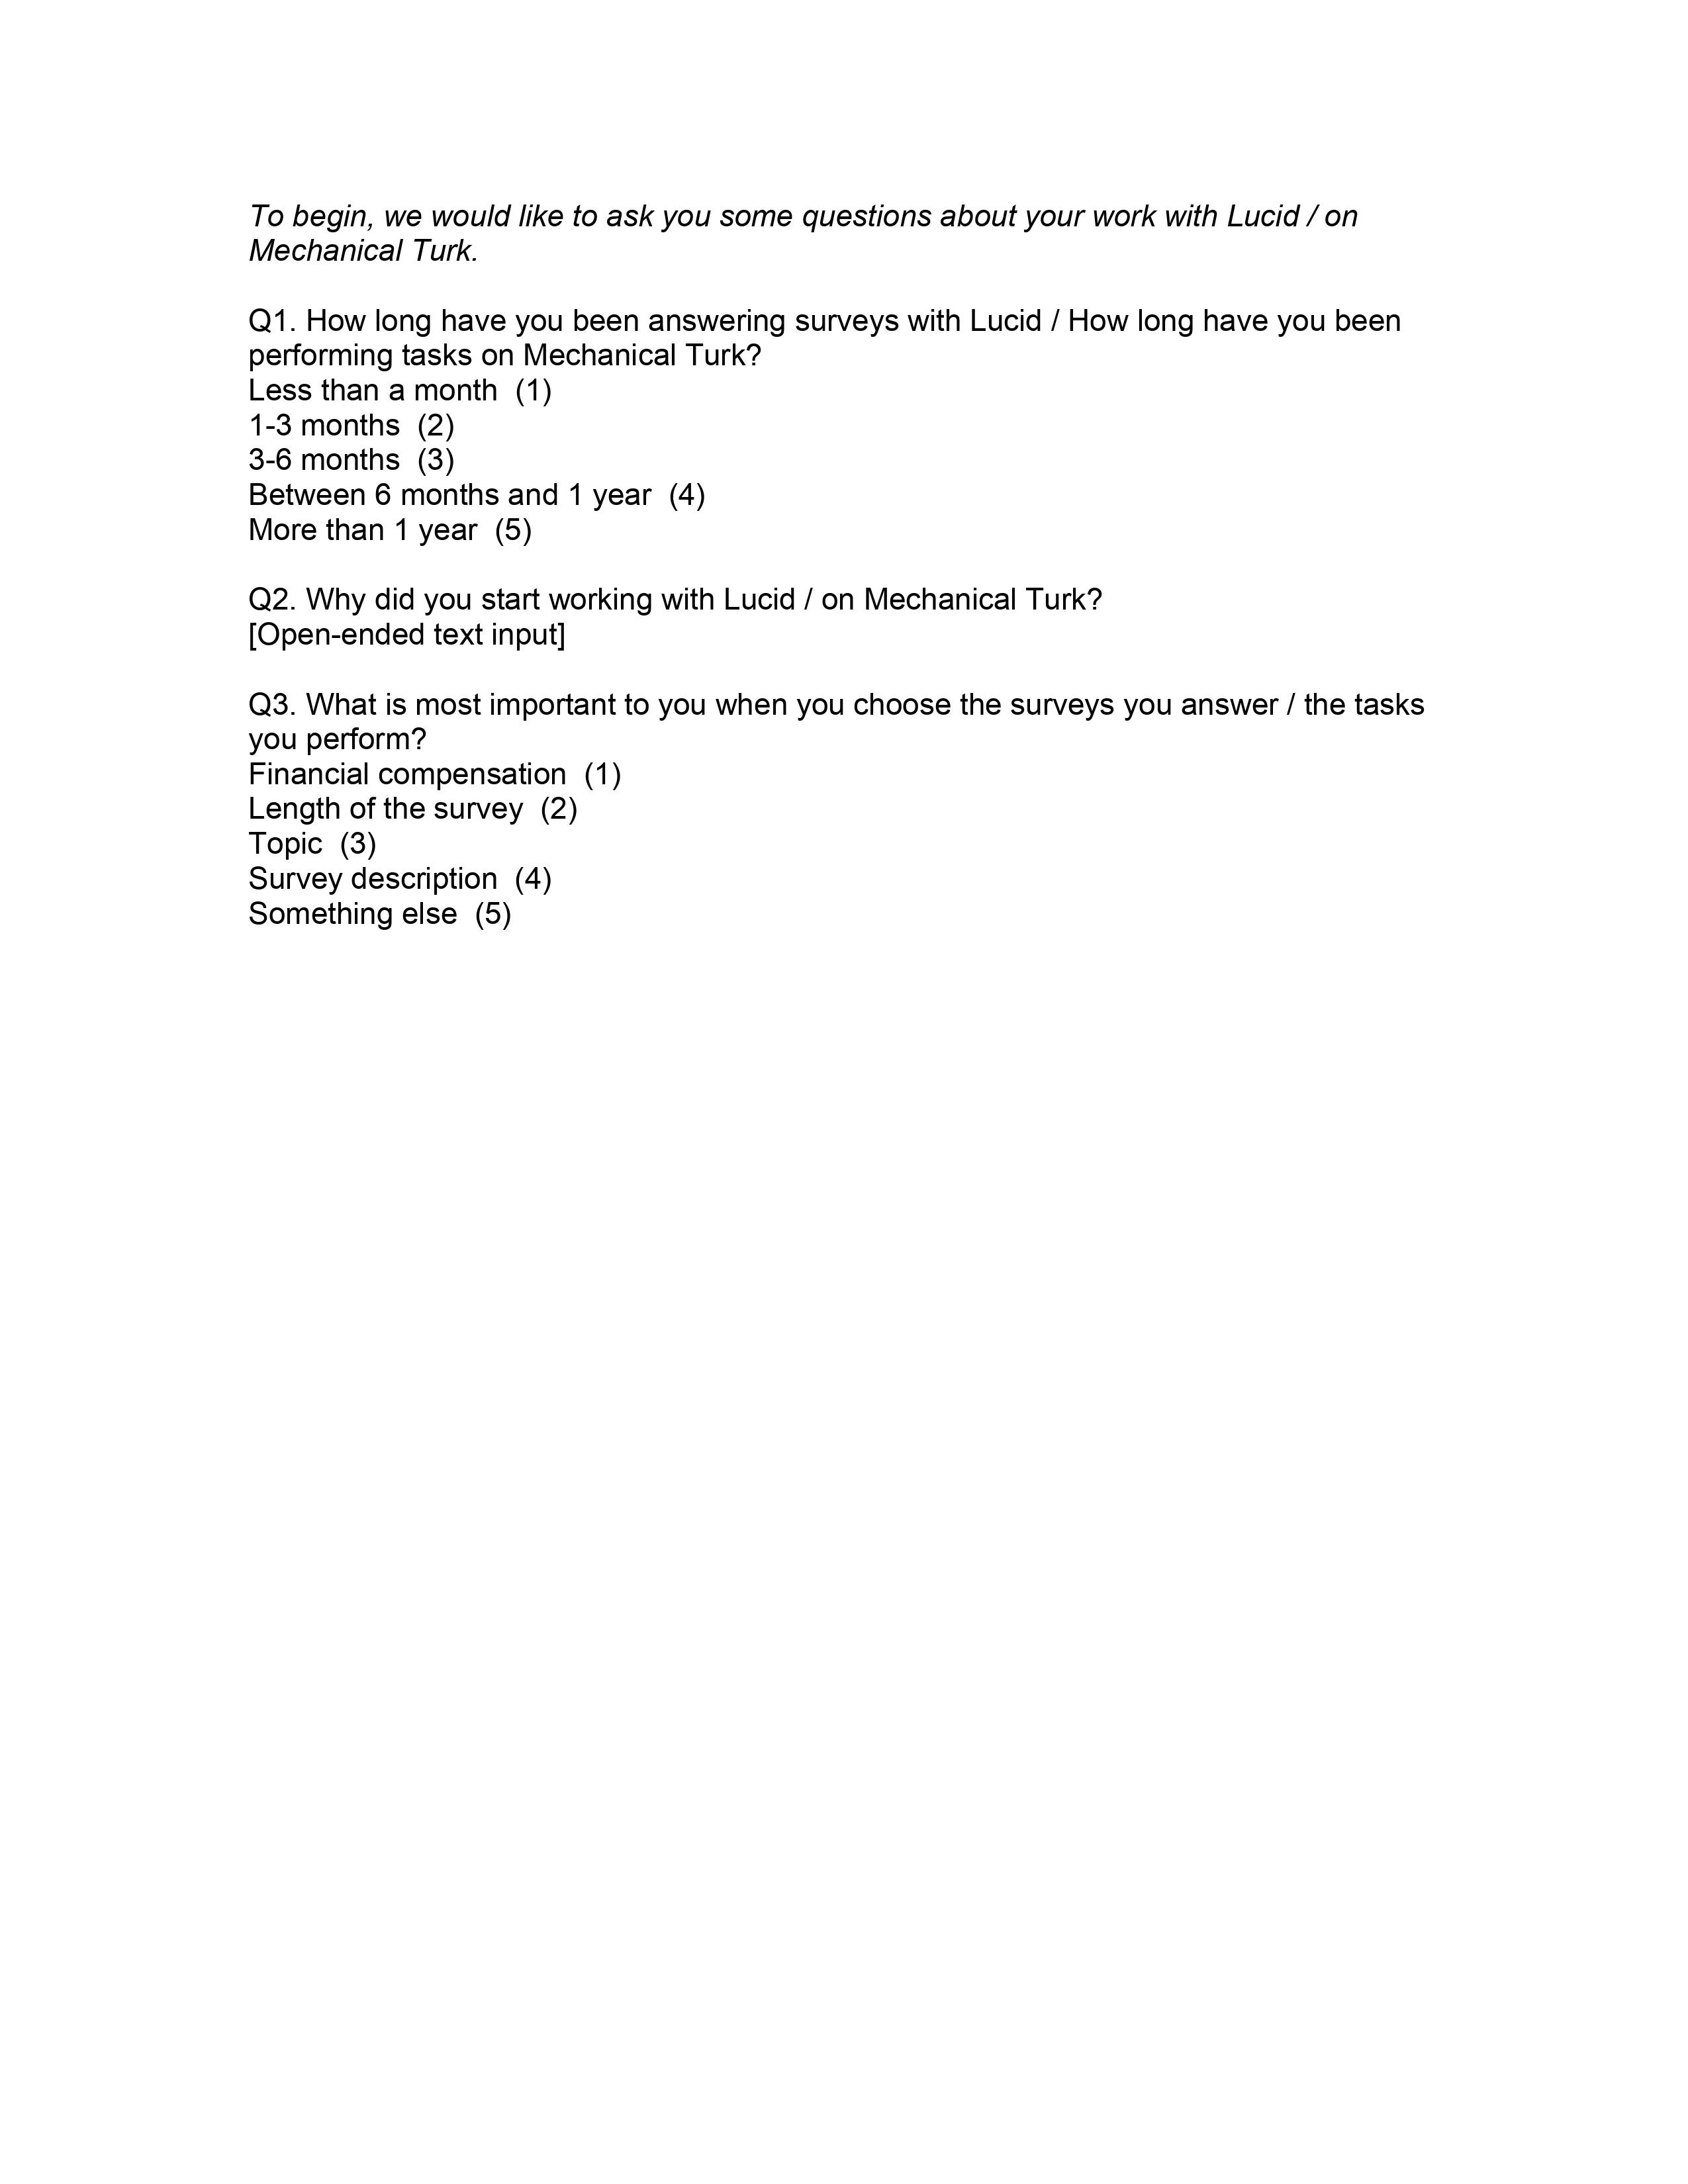
\includegraphics{data/framing/appendix/questionnaire/questionnaire02.jpg}
\end{figure}
\begin{figure}[hbt]
  \centering

\includegraphics{data/framing/appendix/questionnaire/questionnaire03.jpg}
\end{figure}
\begin{figure}[hbt]
  \centering
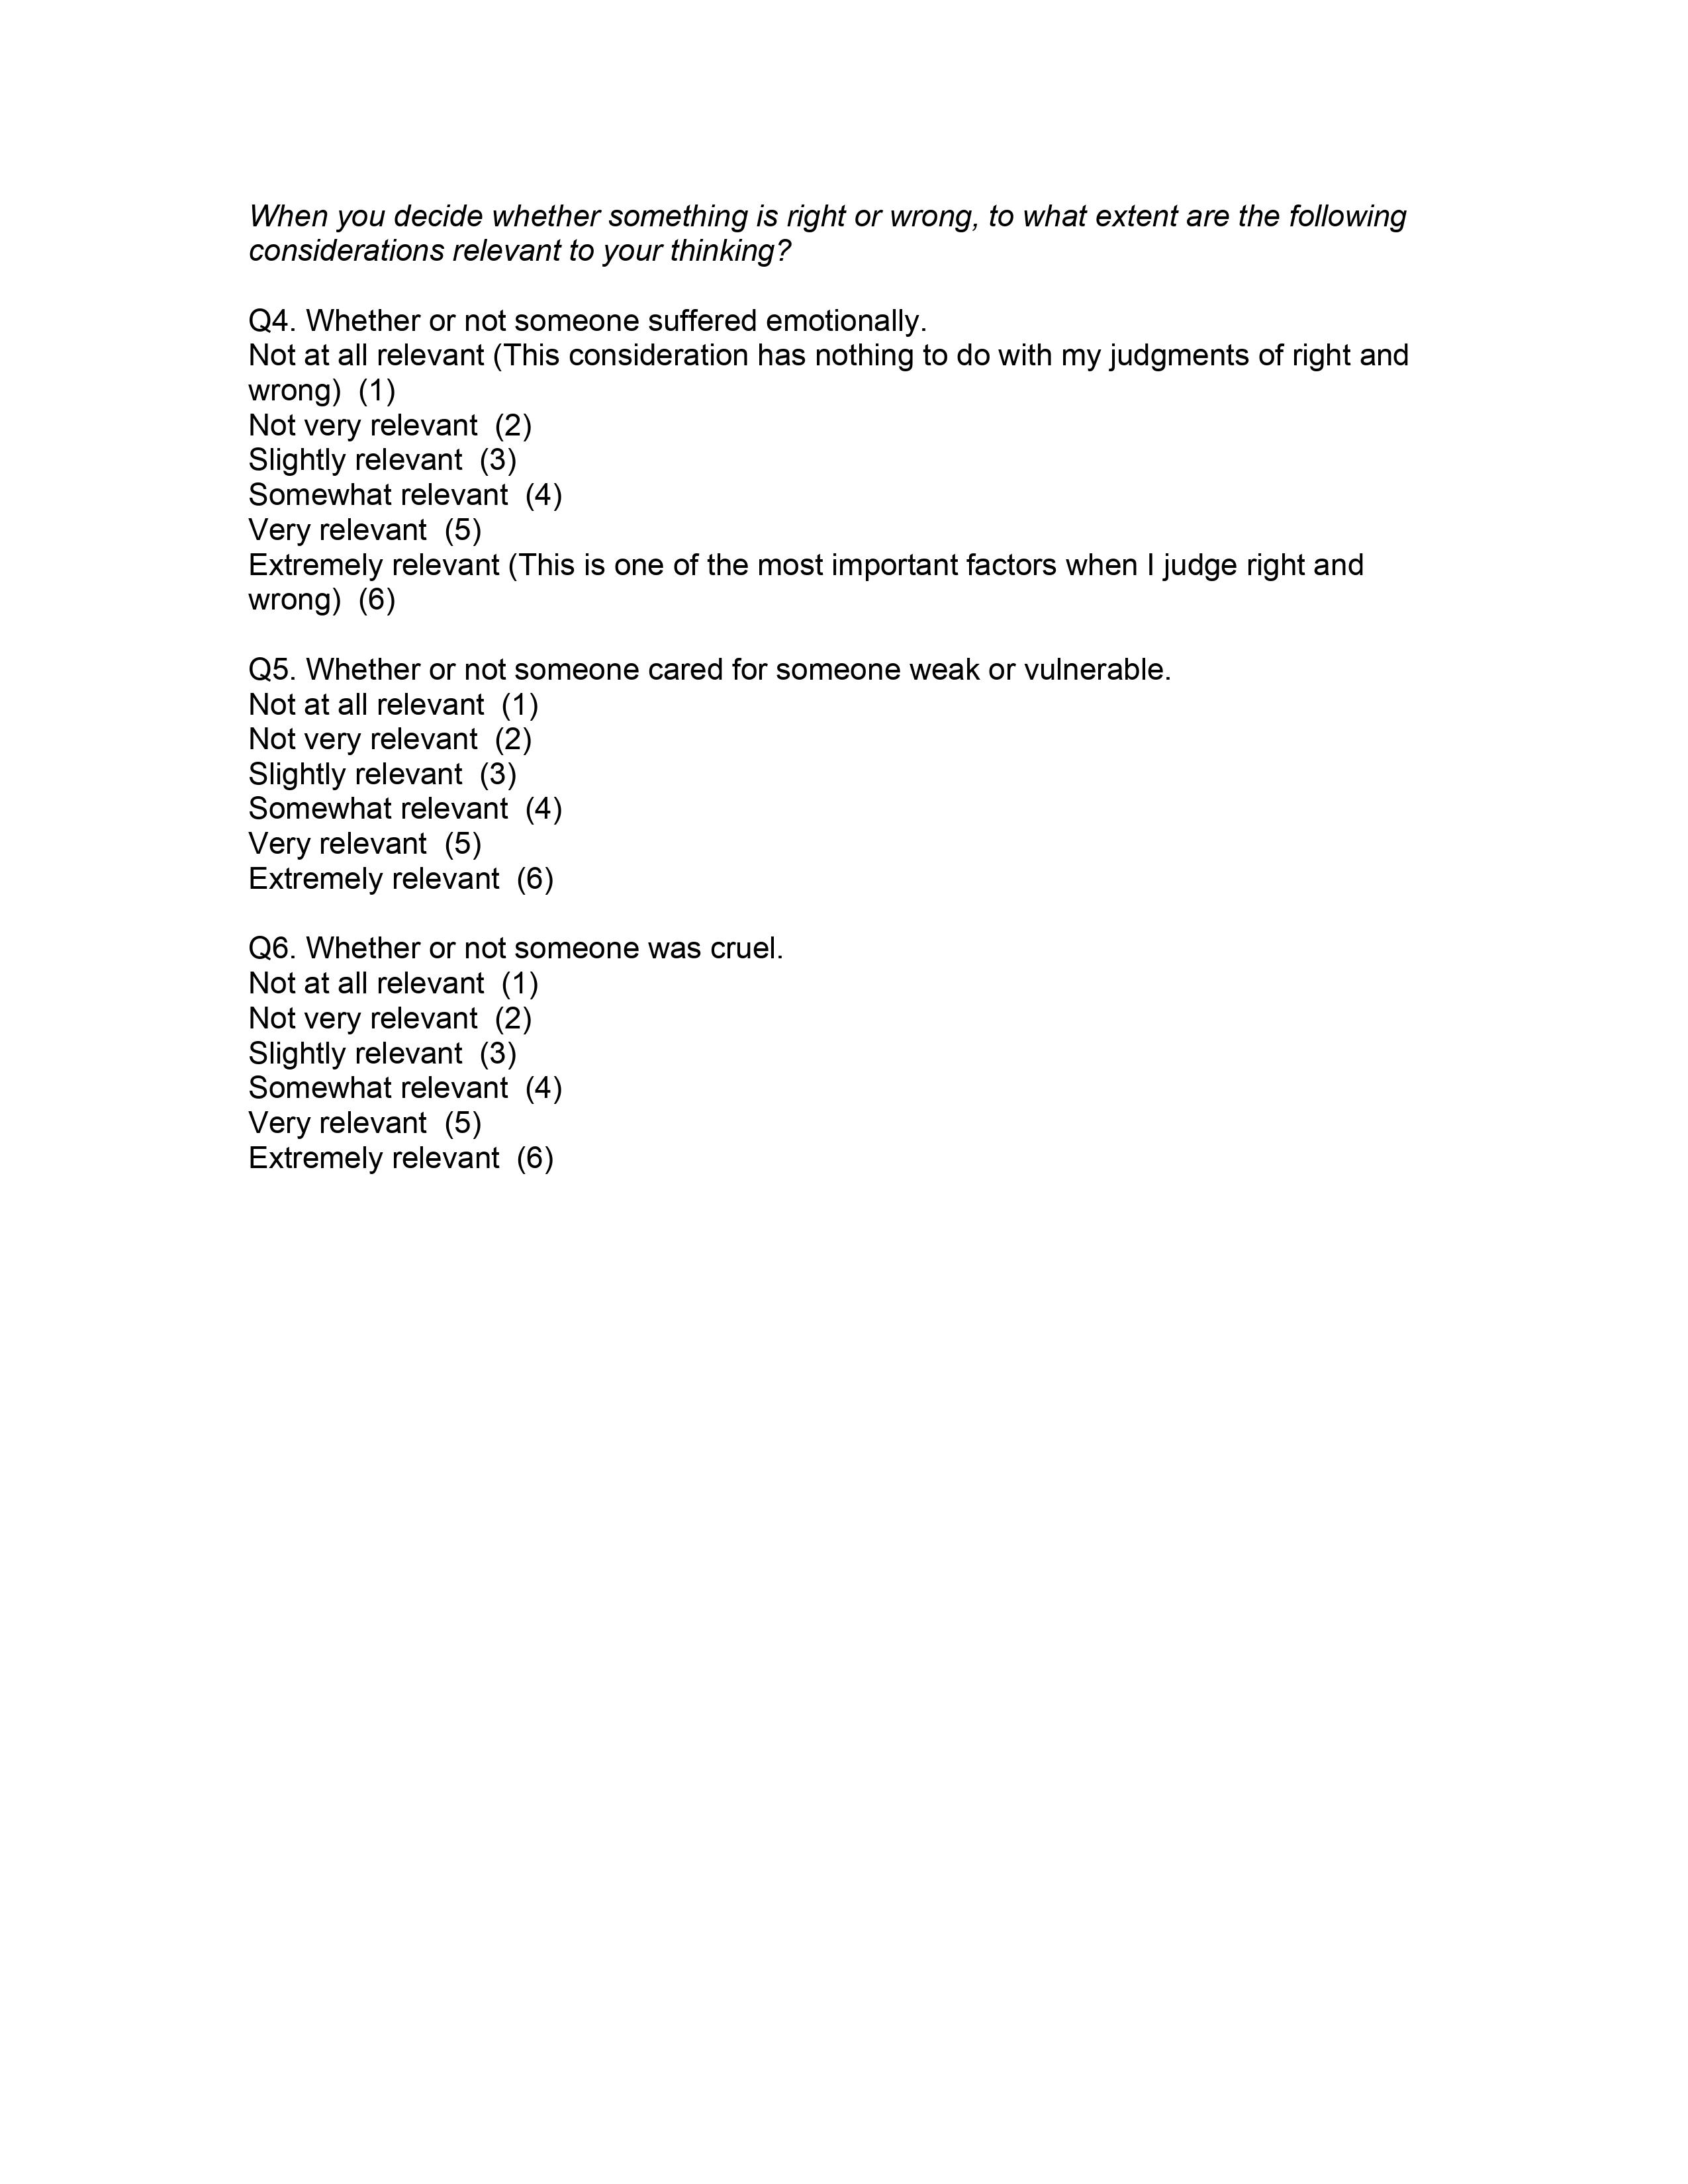
\includegraphics{data/framing/appendix/questionnaire/questionnaire04.jpg}
\end{figure}
\begin{figure}[hbt]
  \centering
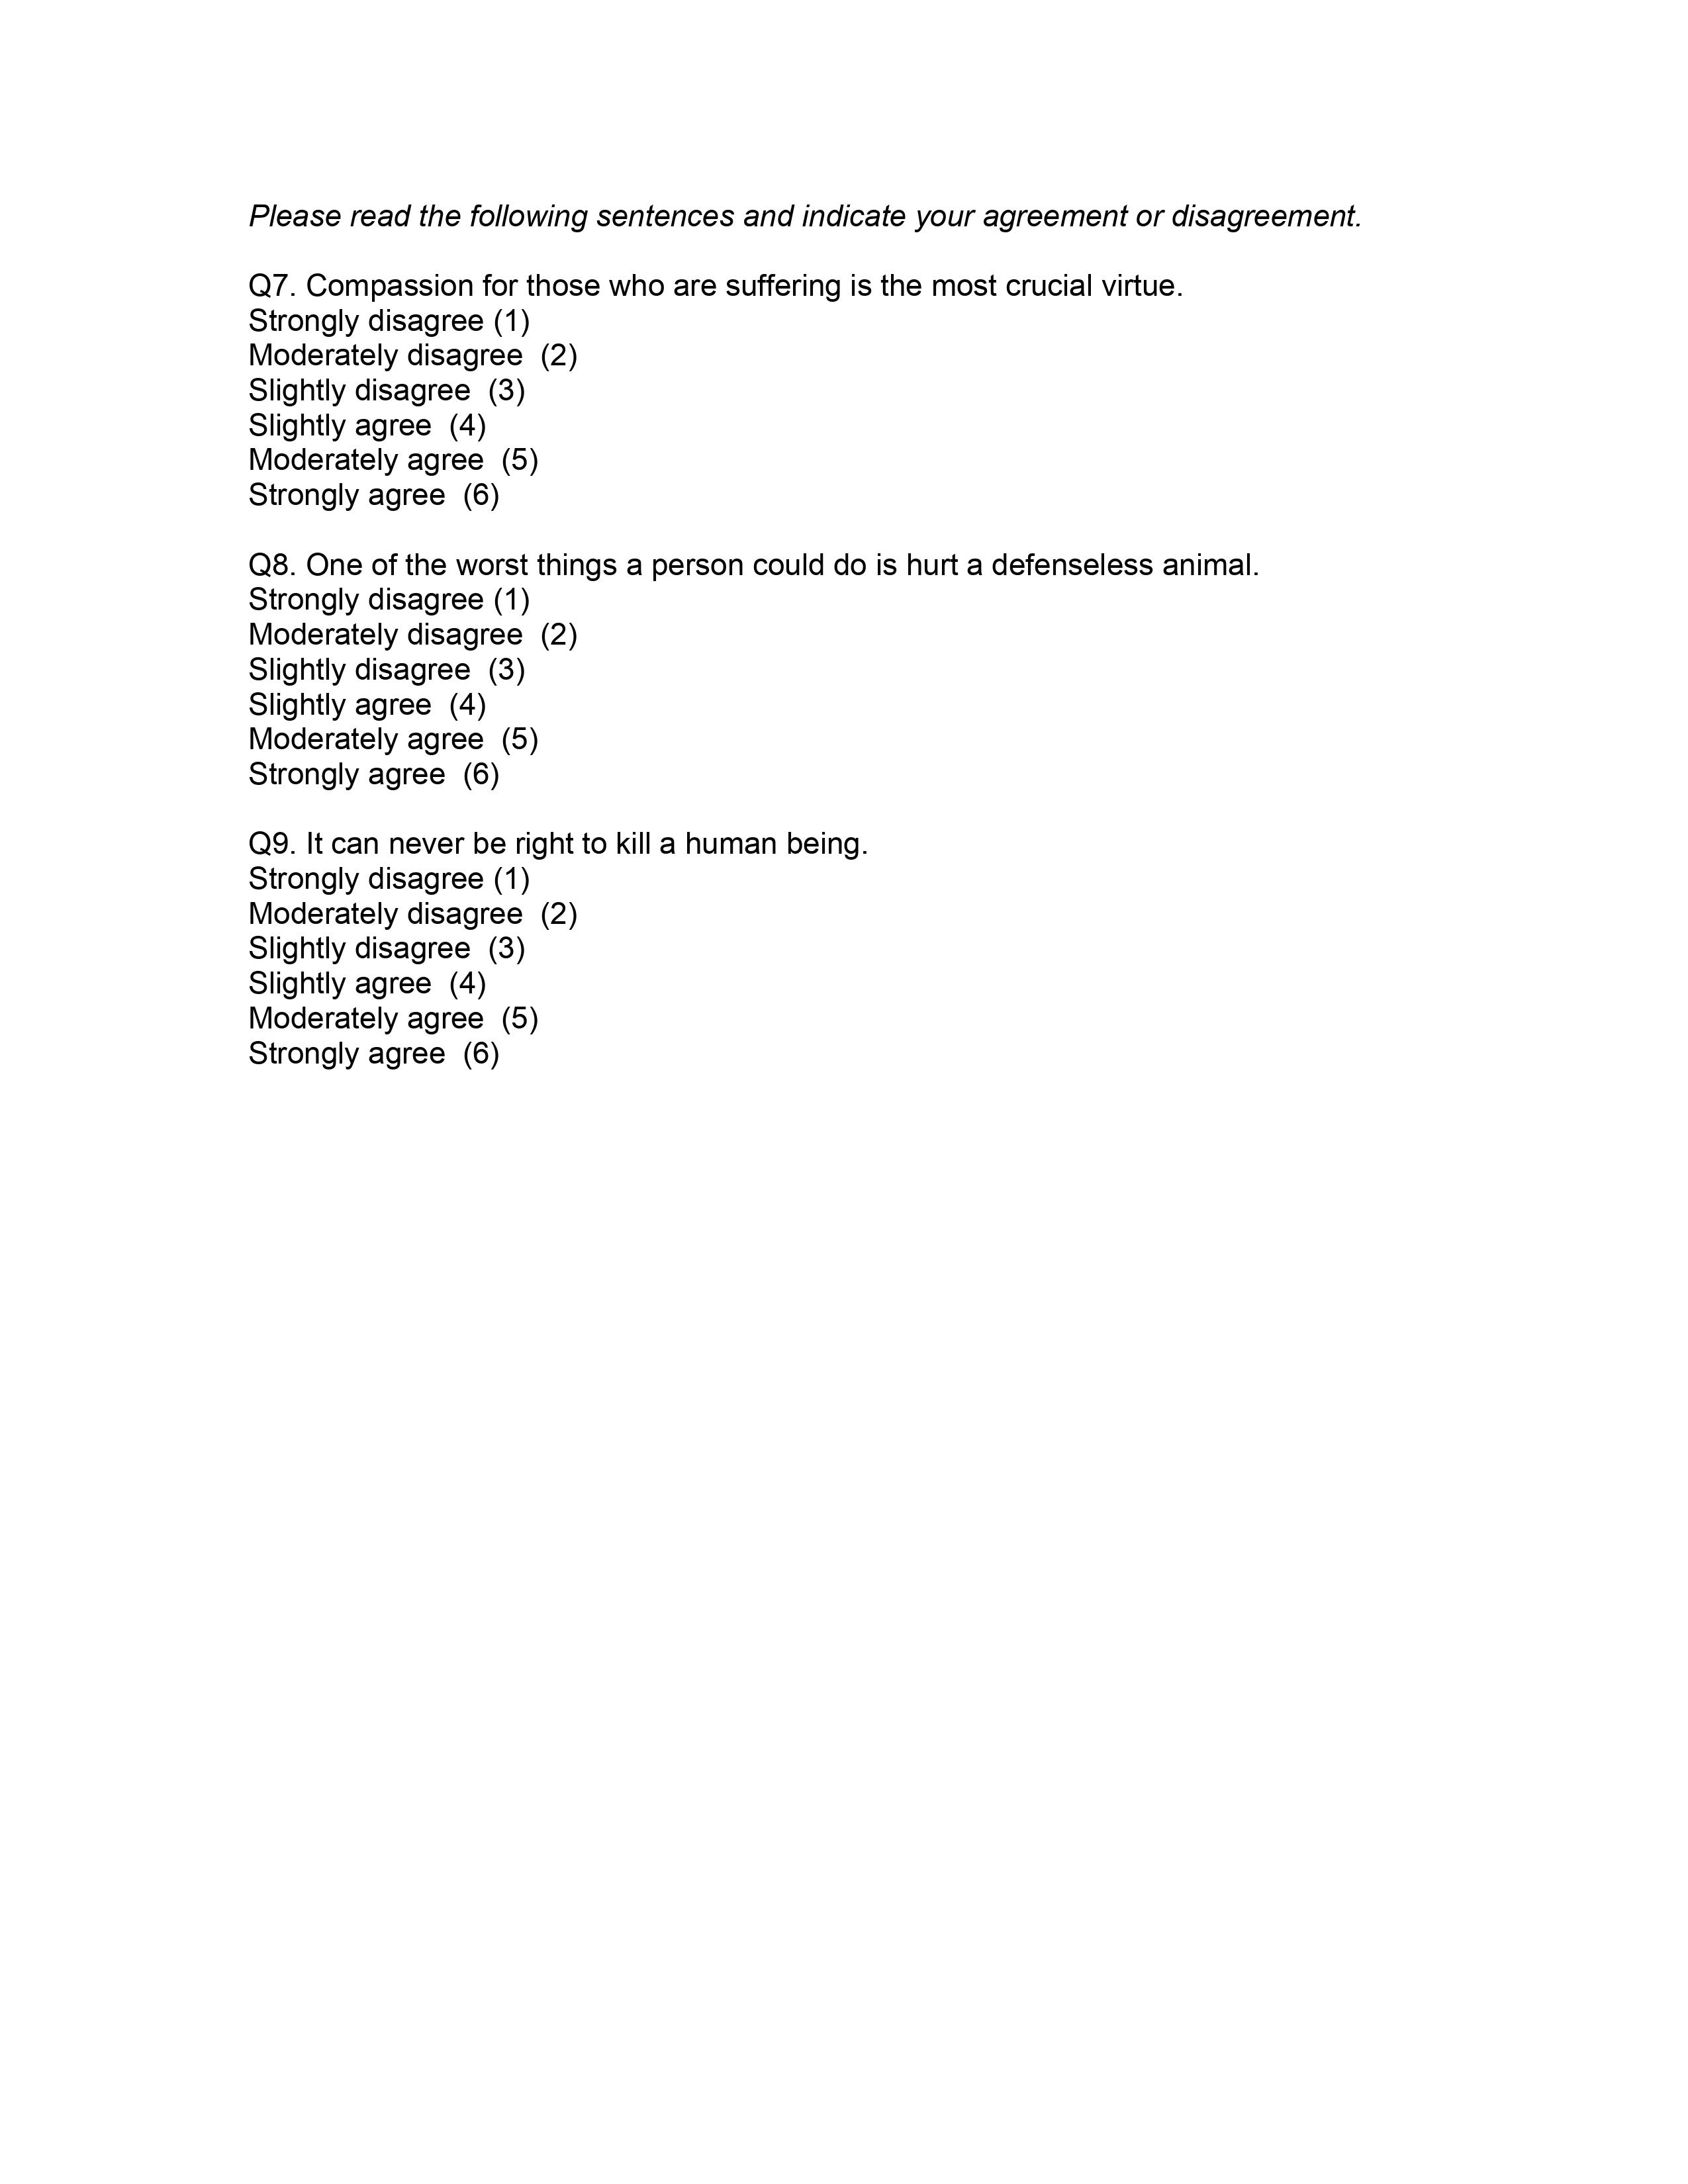
\includegraphics{data/framing/appendix/questionnaire/questionnaire05.jpg}
\end{figure}
\begin{figure}[hbt]
  \centering
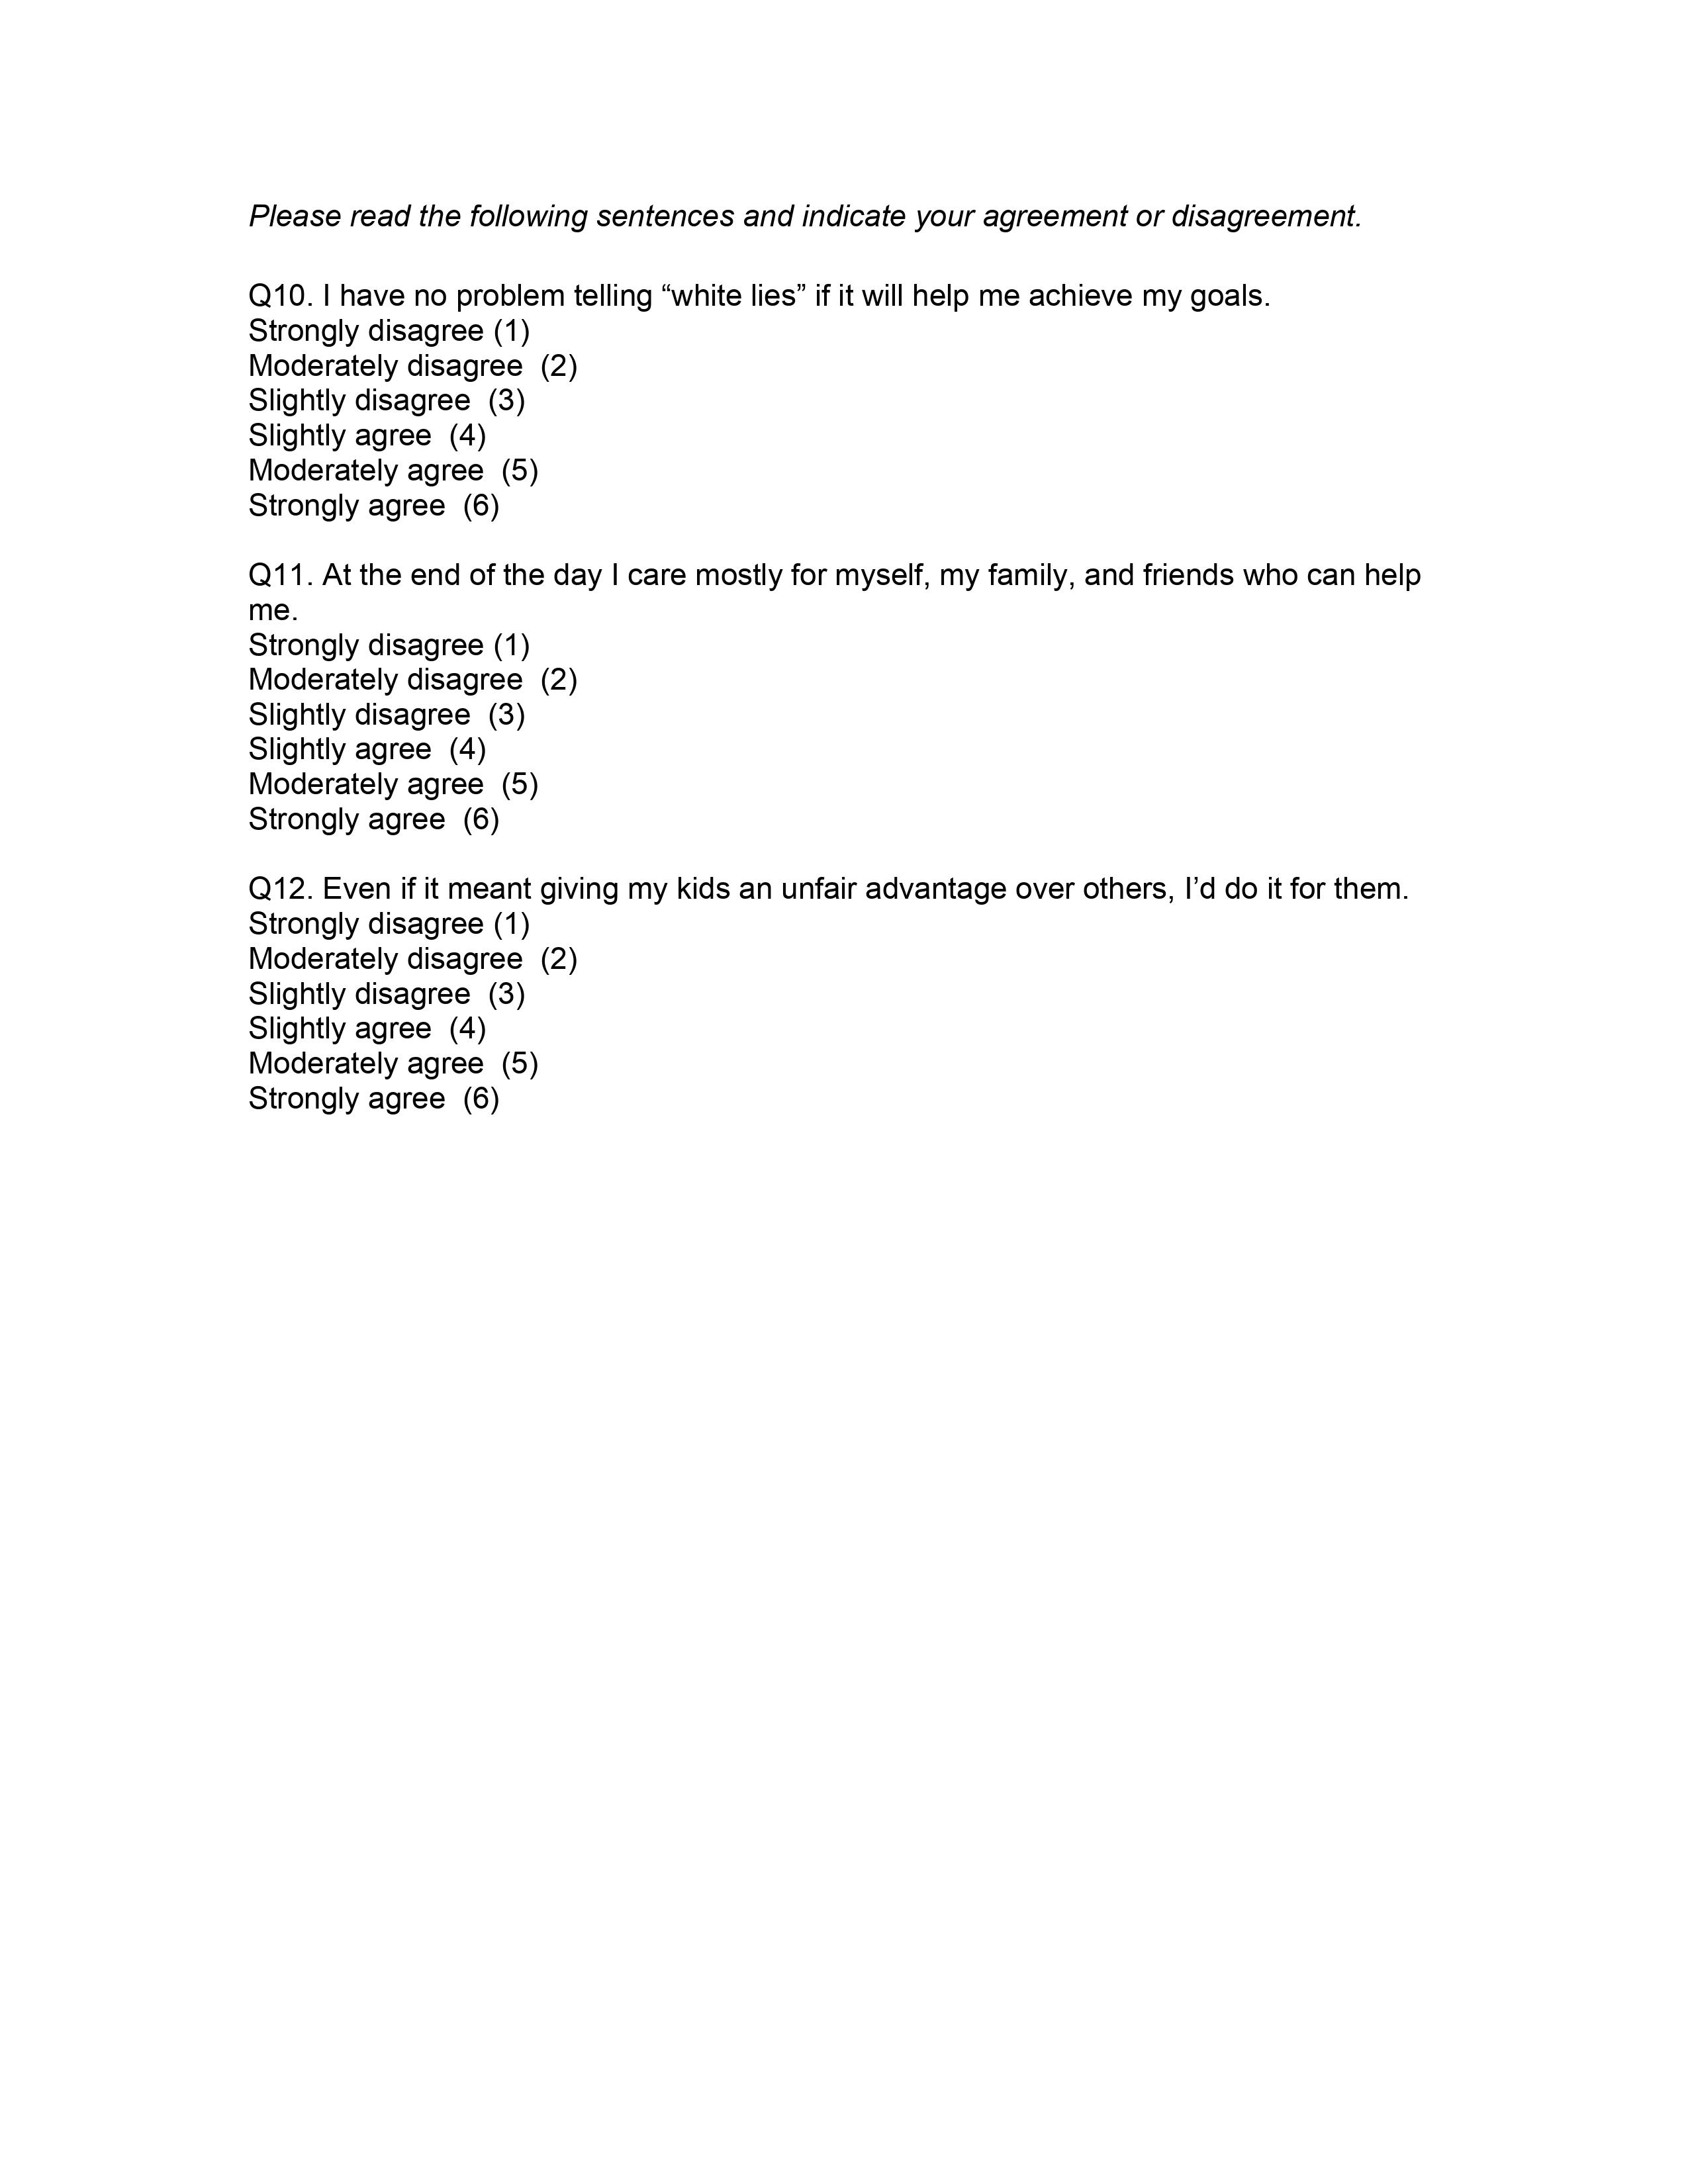
\includegraphics{data/framing/appendix/questionnaire/questionnaire06.jpg}
\end{figure}
\begin{figure}[hbt]
  \centering
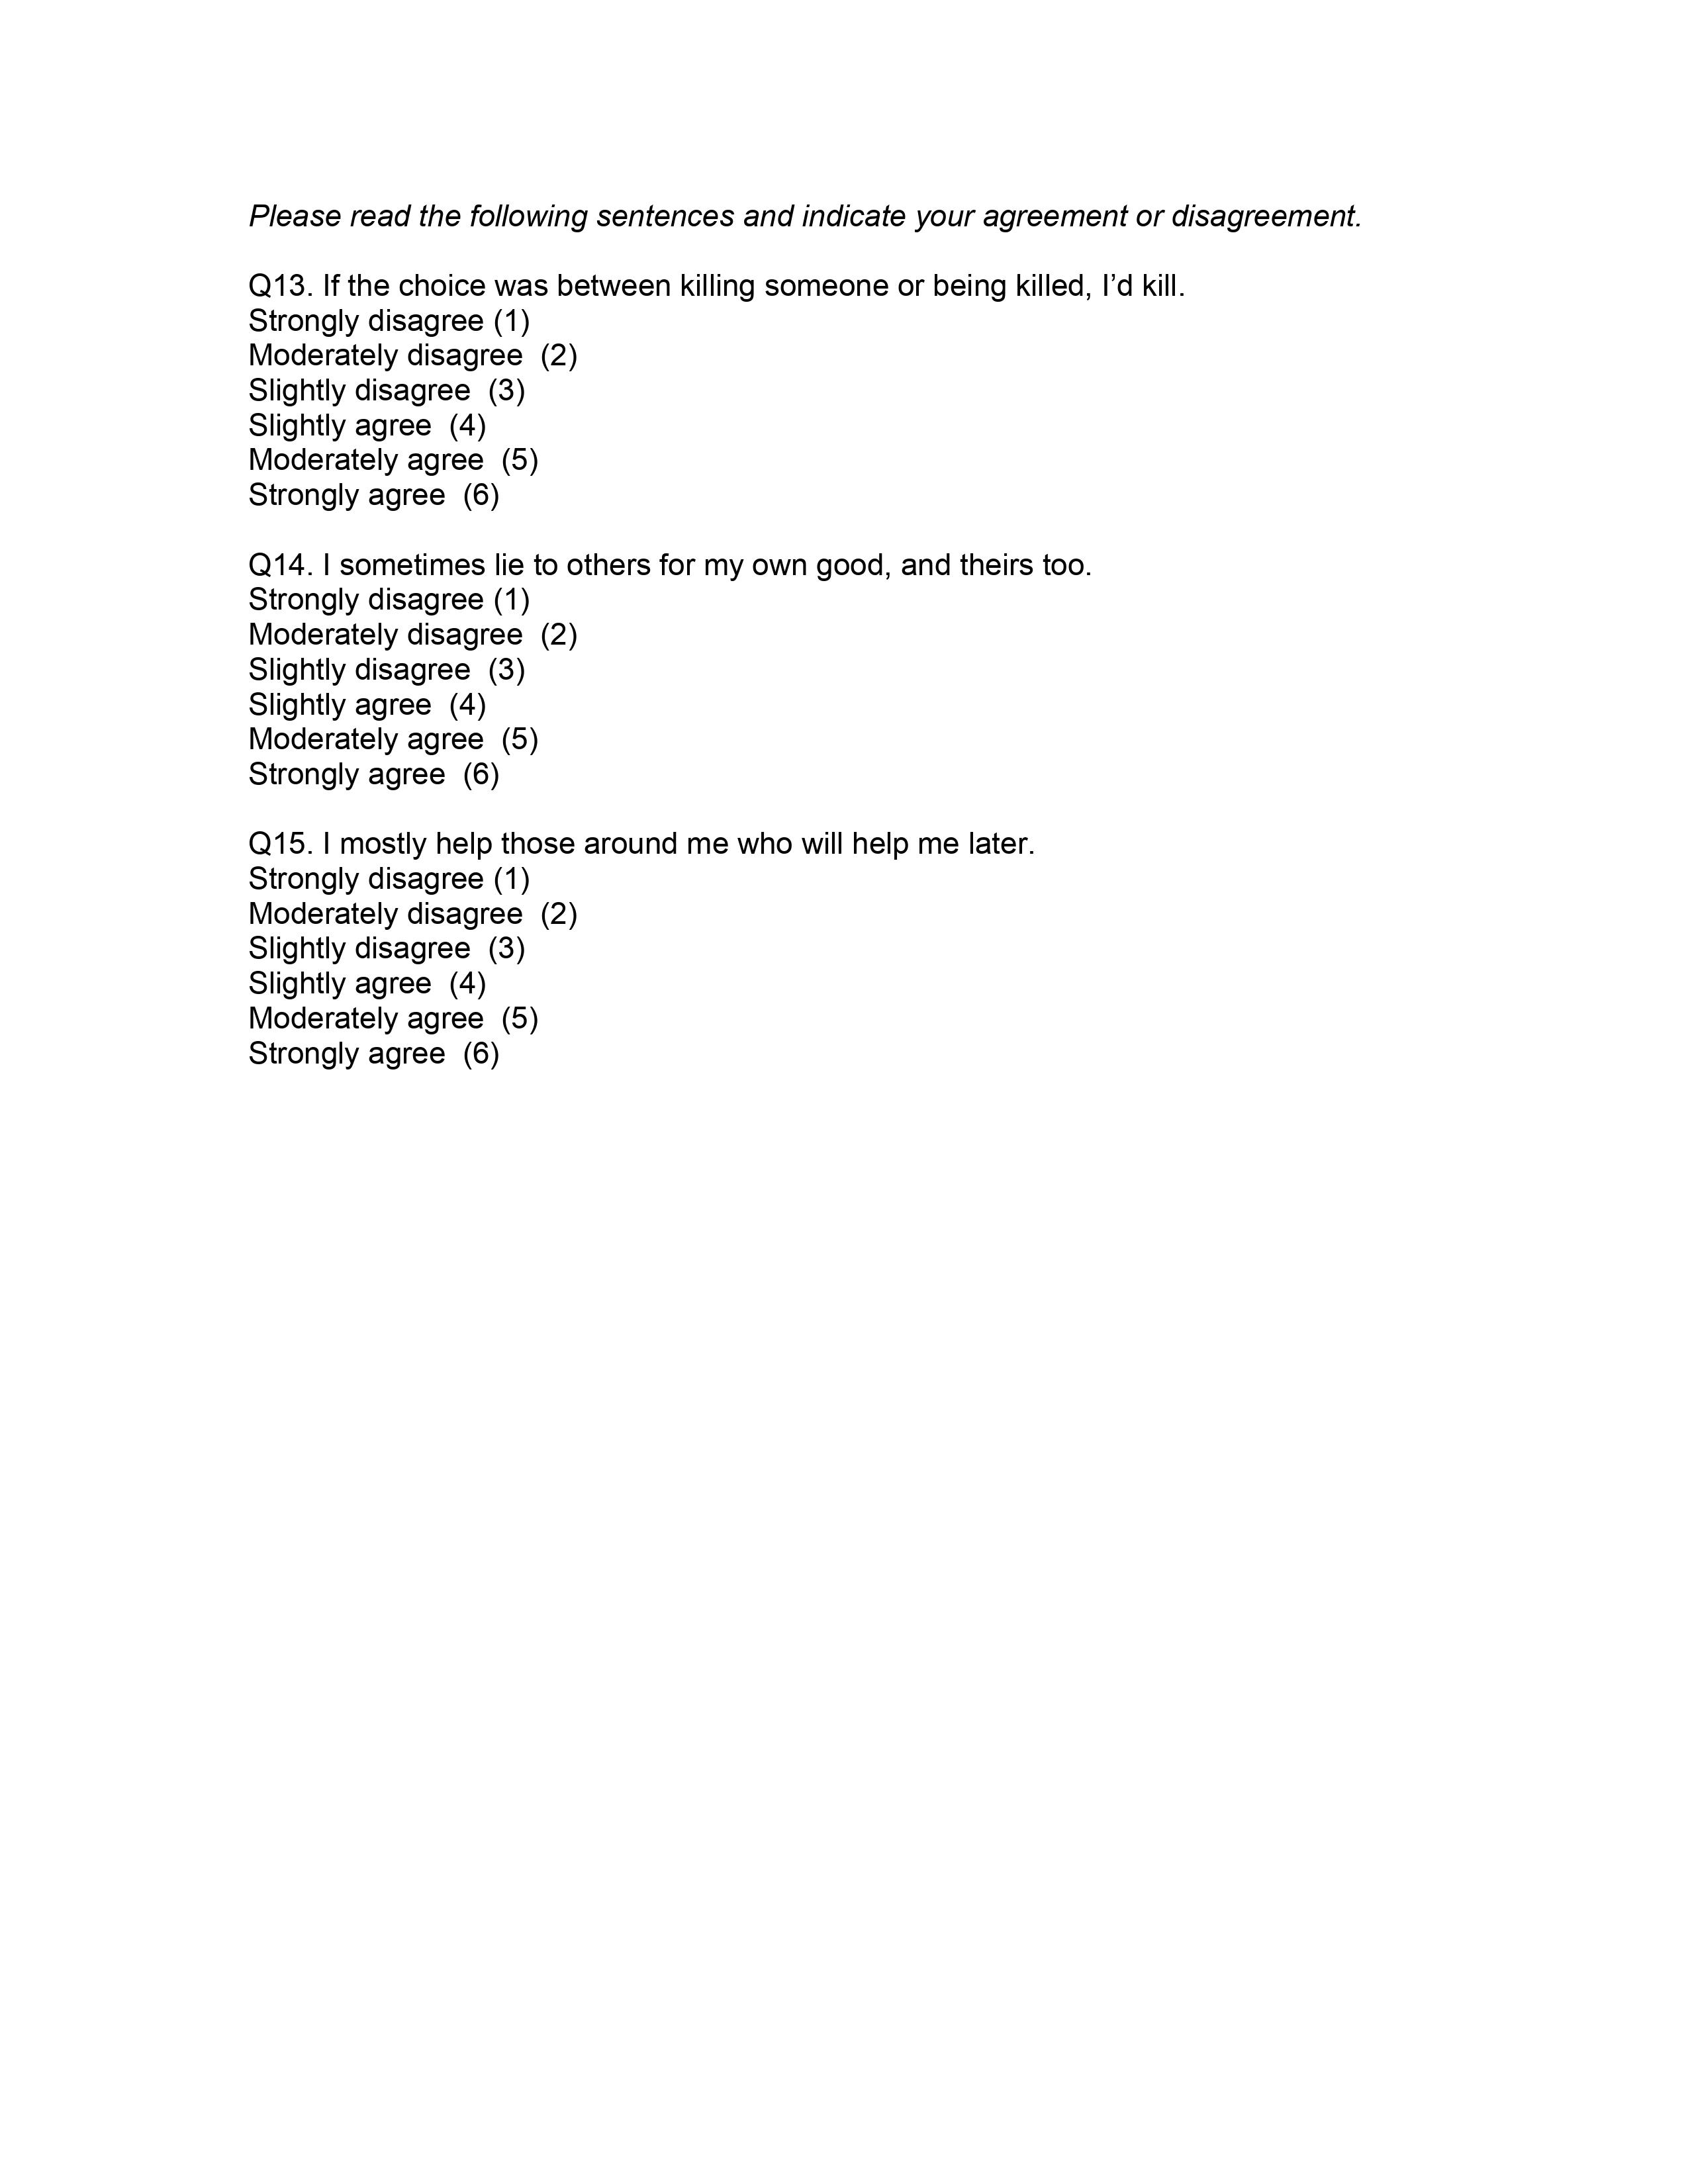
\includegraphics{data/framing/appendix/questionnaire/questionnaire07.jpg}
\end{figure}
\begin{figure}[hbt]
  \centering

\includegraphics{data/framing/appendix/questionnaire/questionnaire08.jpg}
\end{figure}
\begin{figure}[hbt]
  \centering
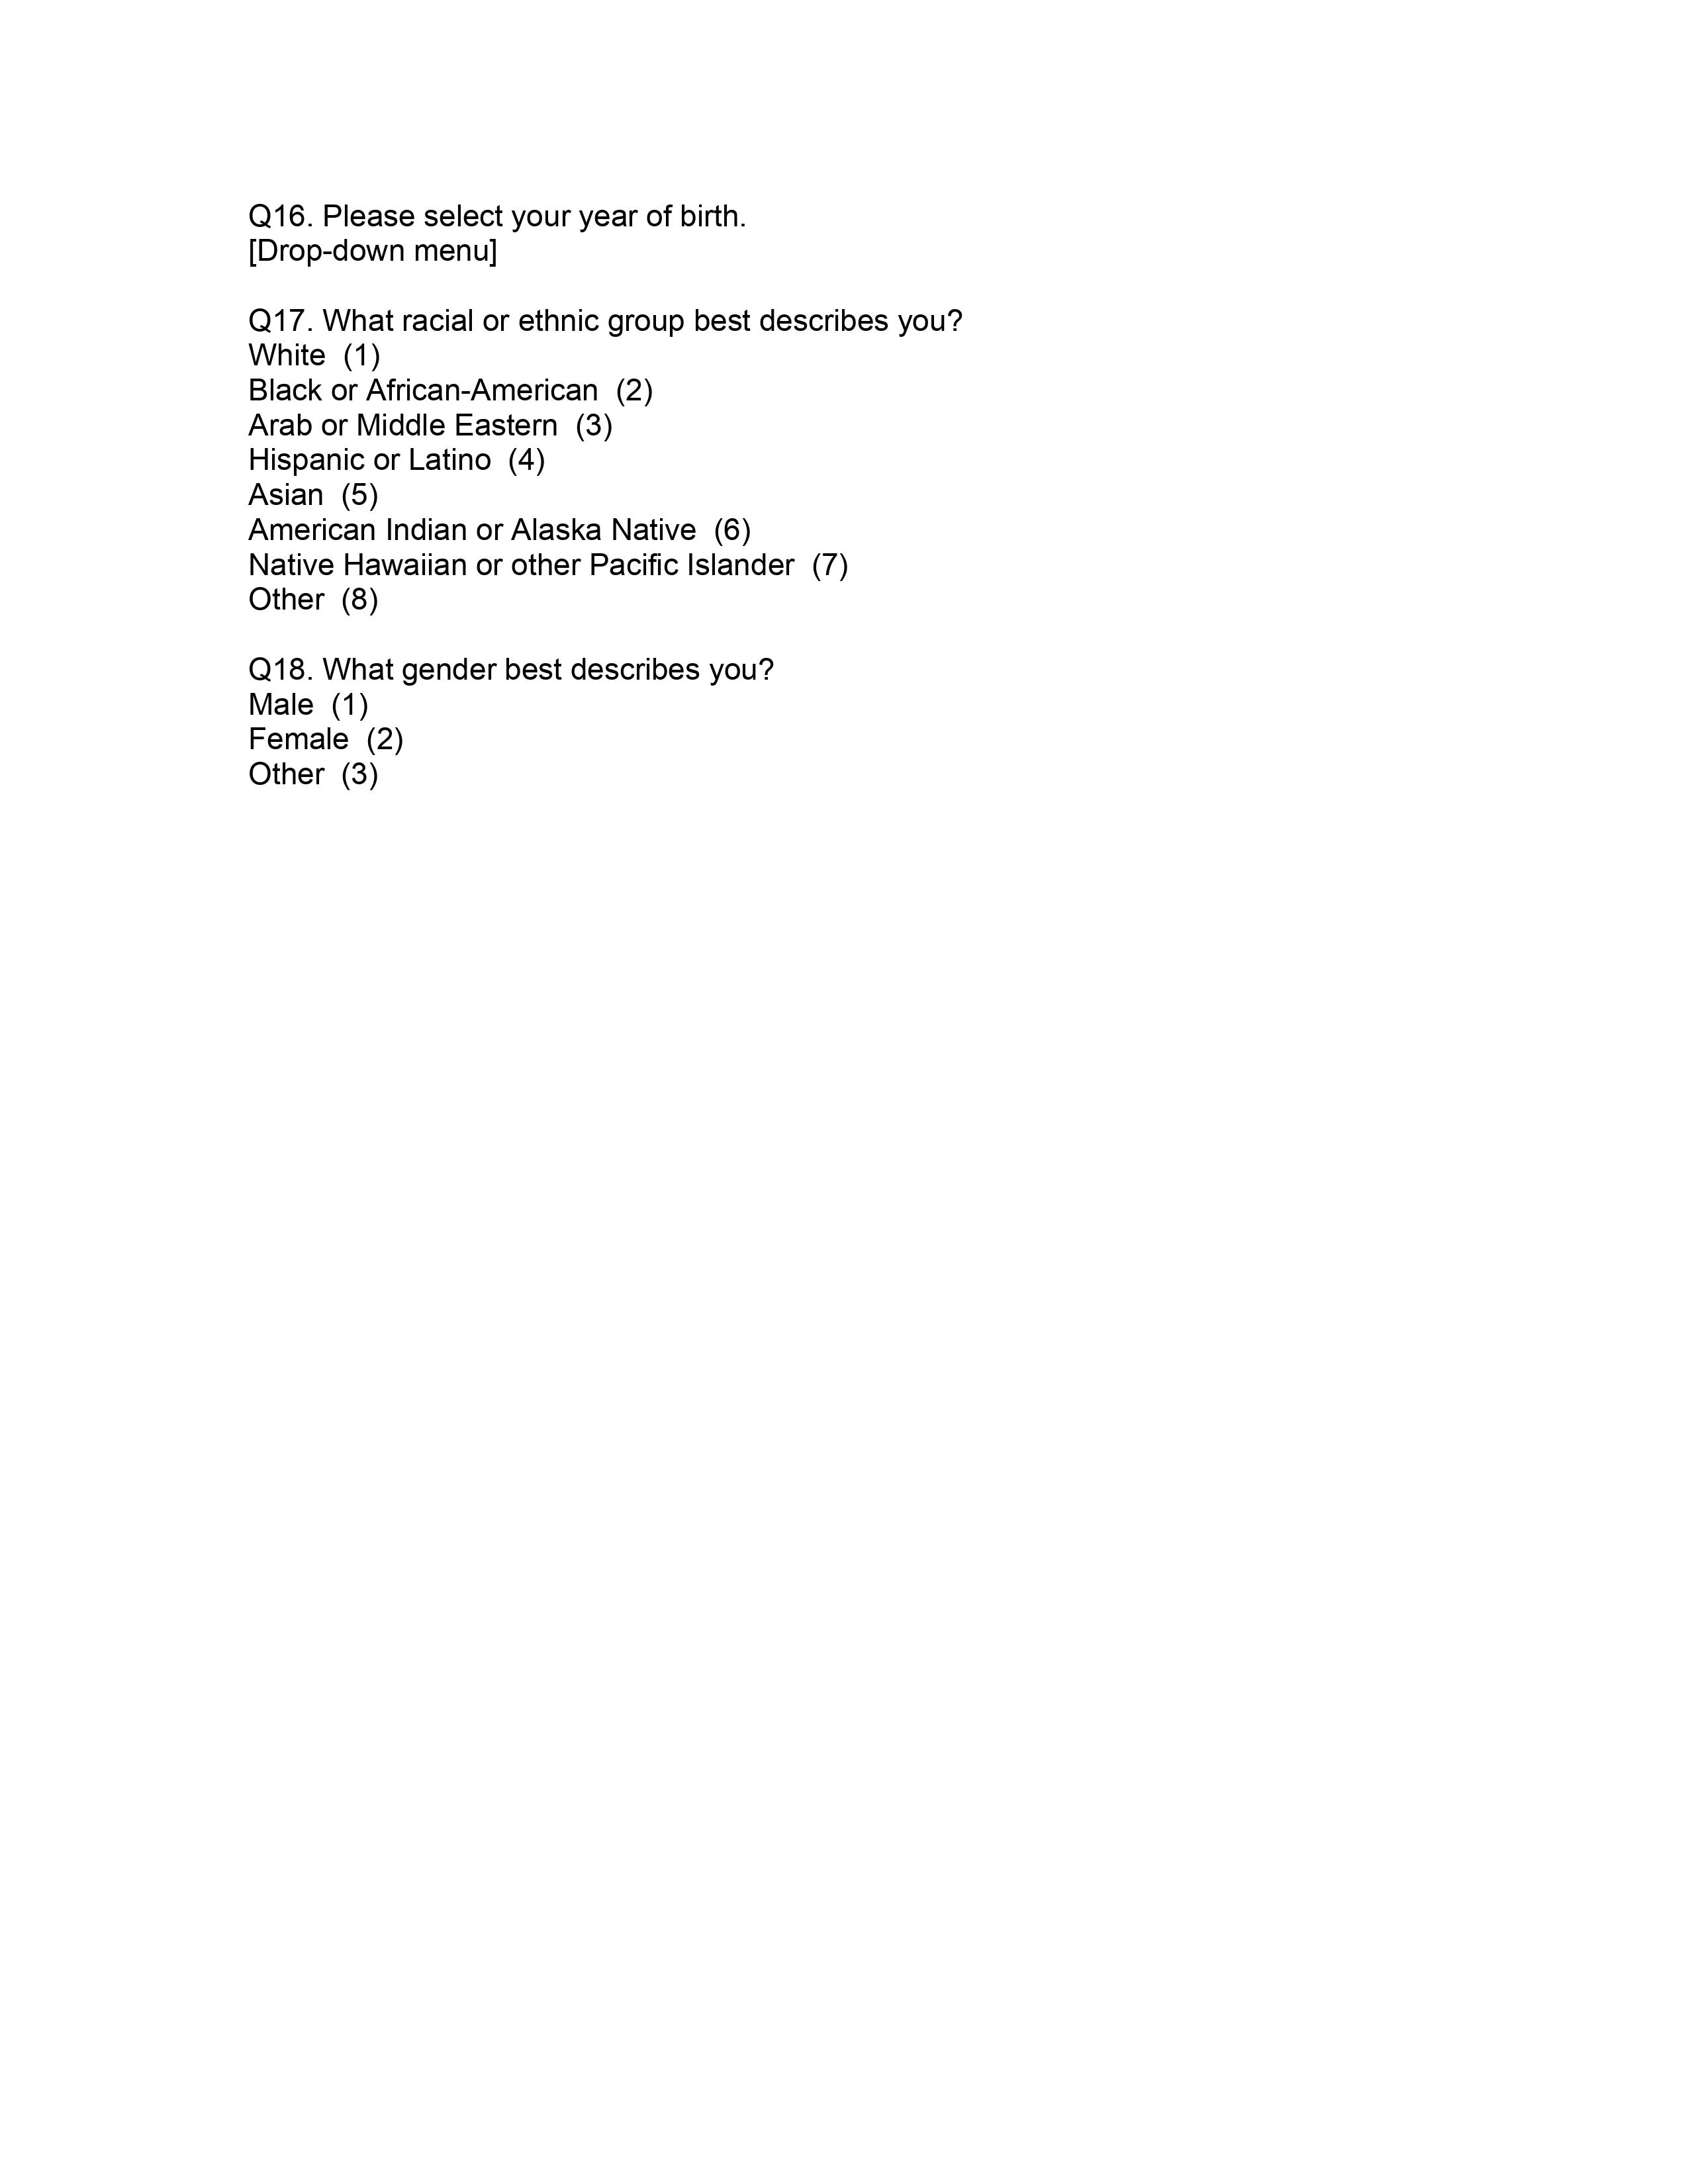
\includegraphics{data/framing/appendix/questionnaire/questionnaire09.jpg}
\end{figure}
\begin{figure}[hbt]
  \centering
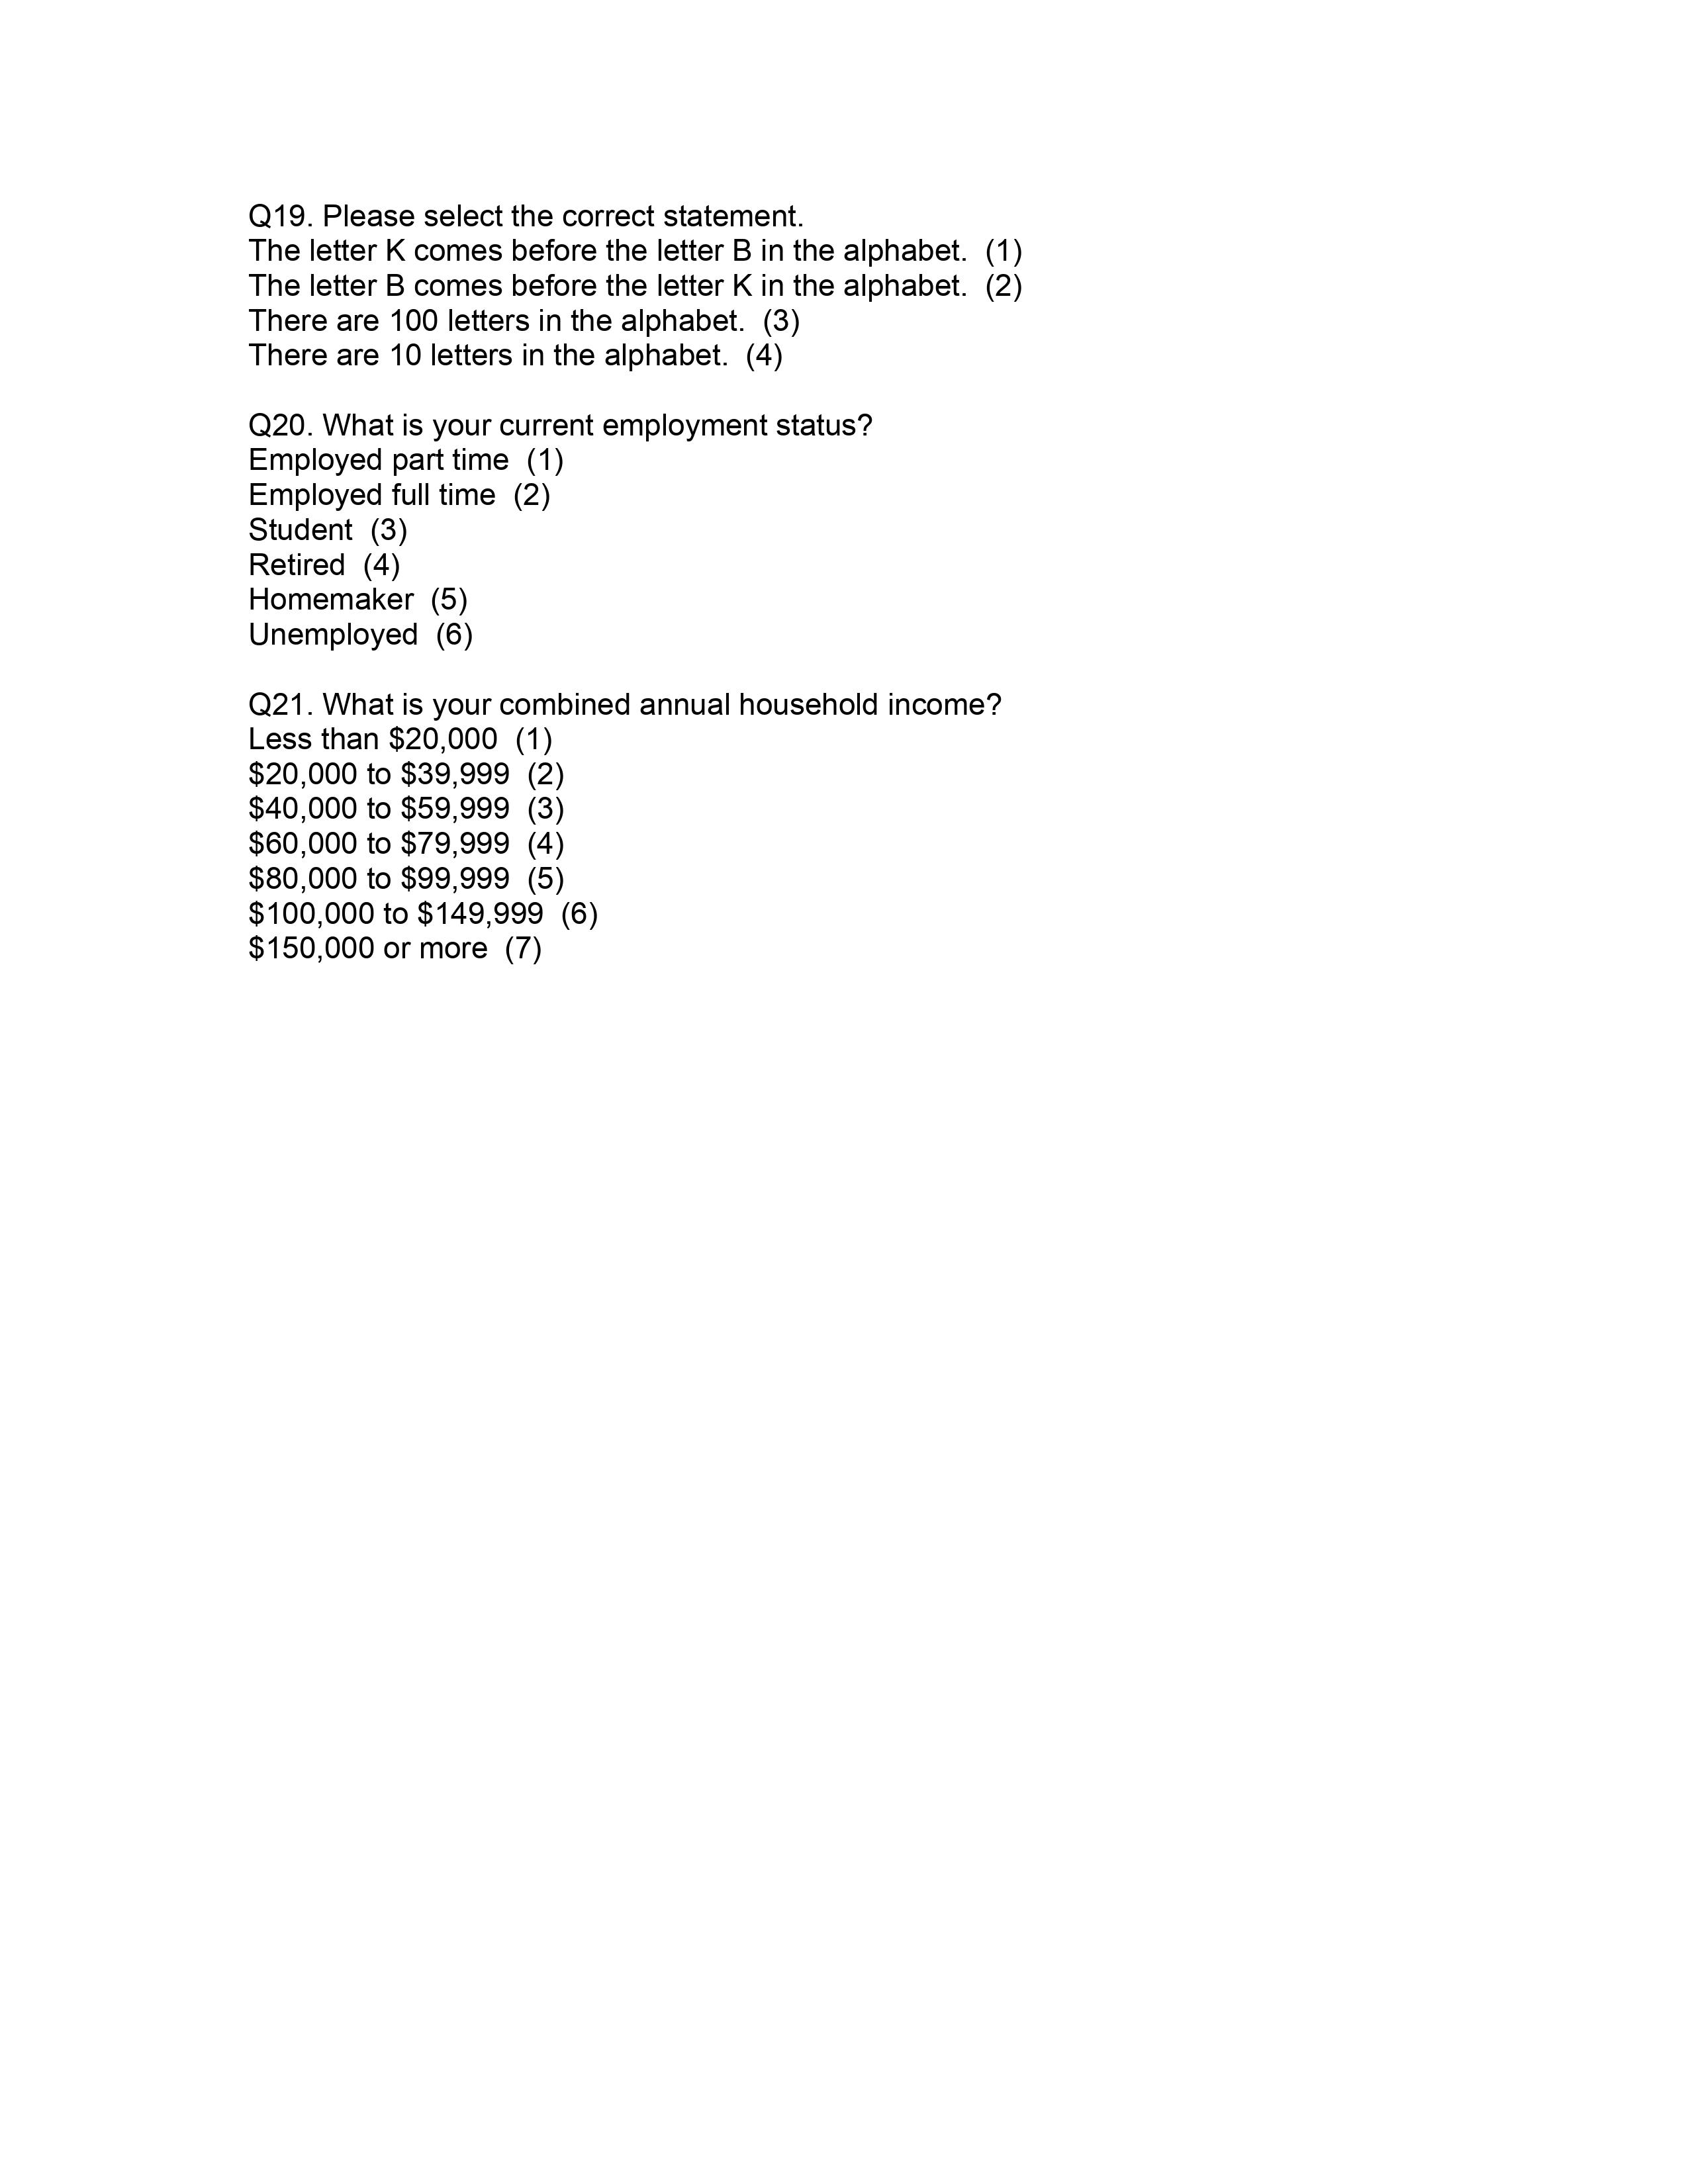
\includegraphics{data/framing/appendix/questionnaire/questionnaire10.jpg}
\end{figure}
\begin{figure}[hbt]
  \centering

\includegraphics{data/framing/appendix/questionnaire/questionnaire11.jpg}
\end{figure}
\begin{figure}[hbt]
  \centering
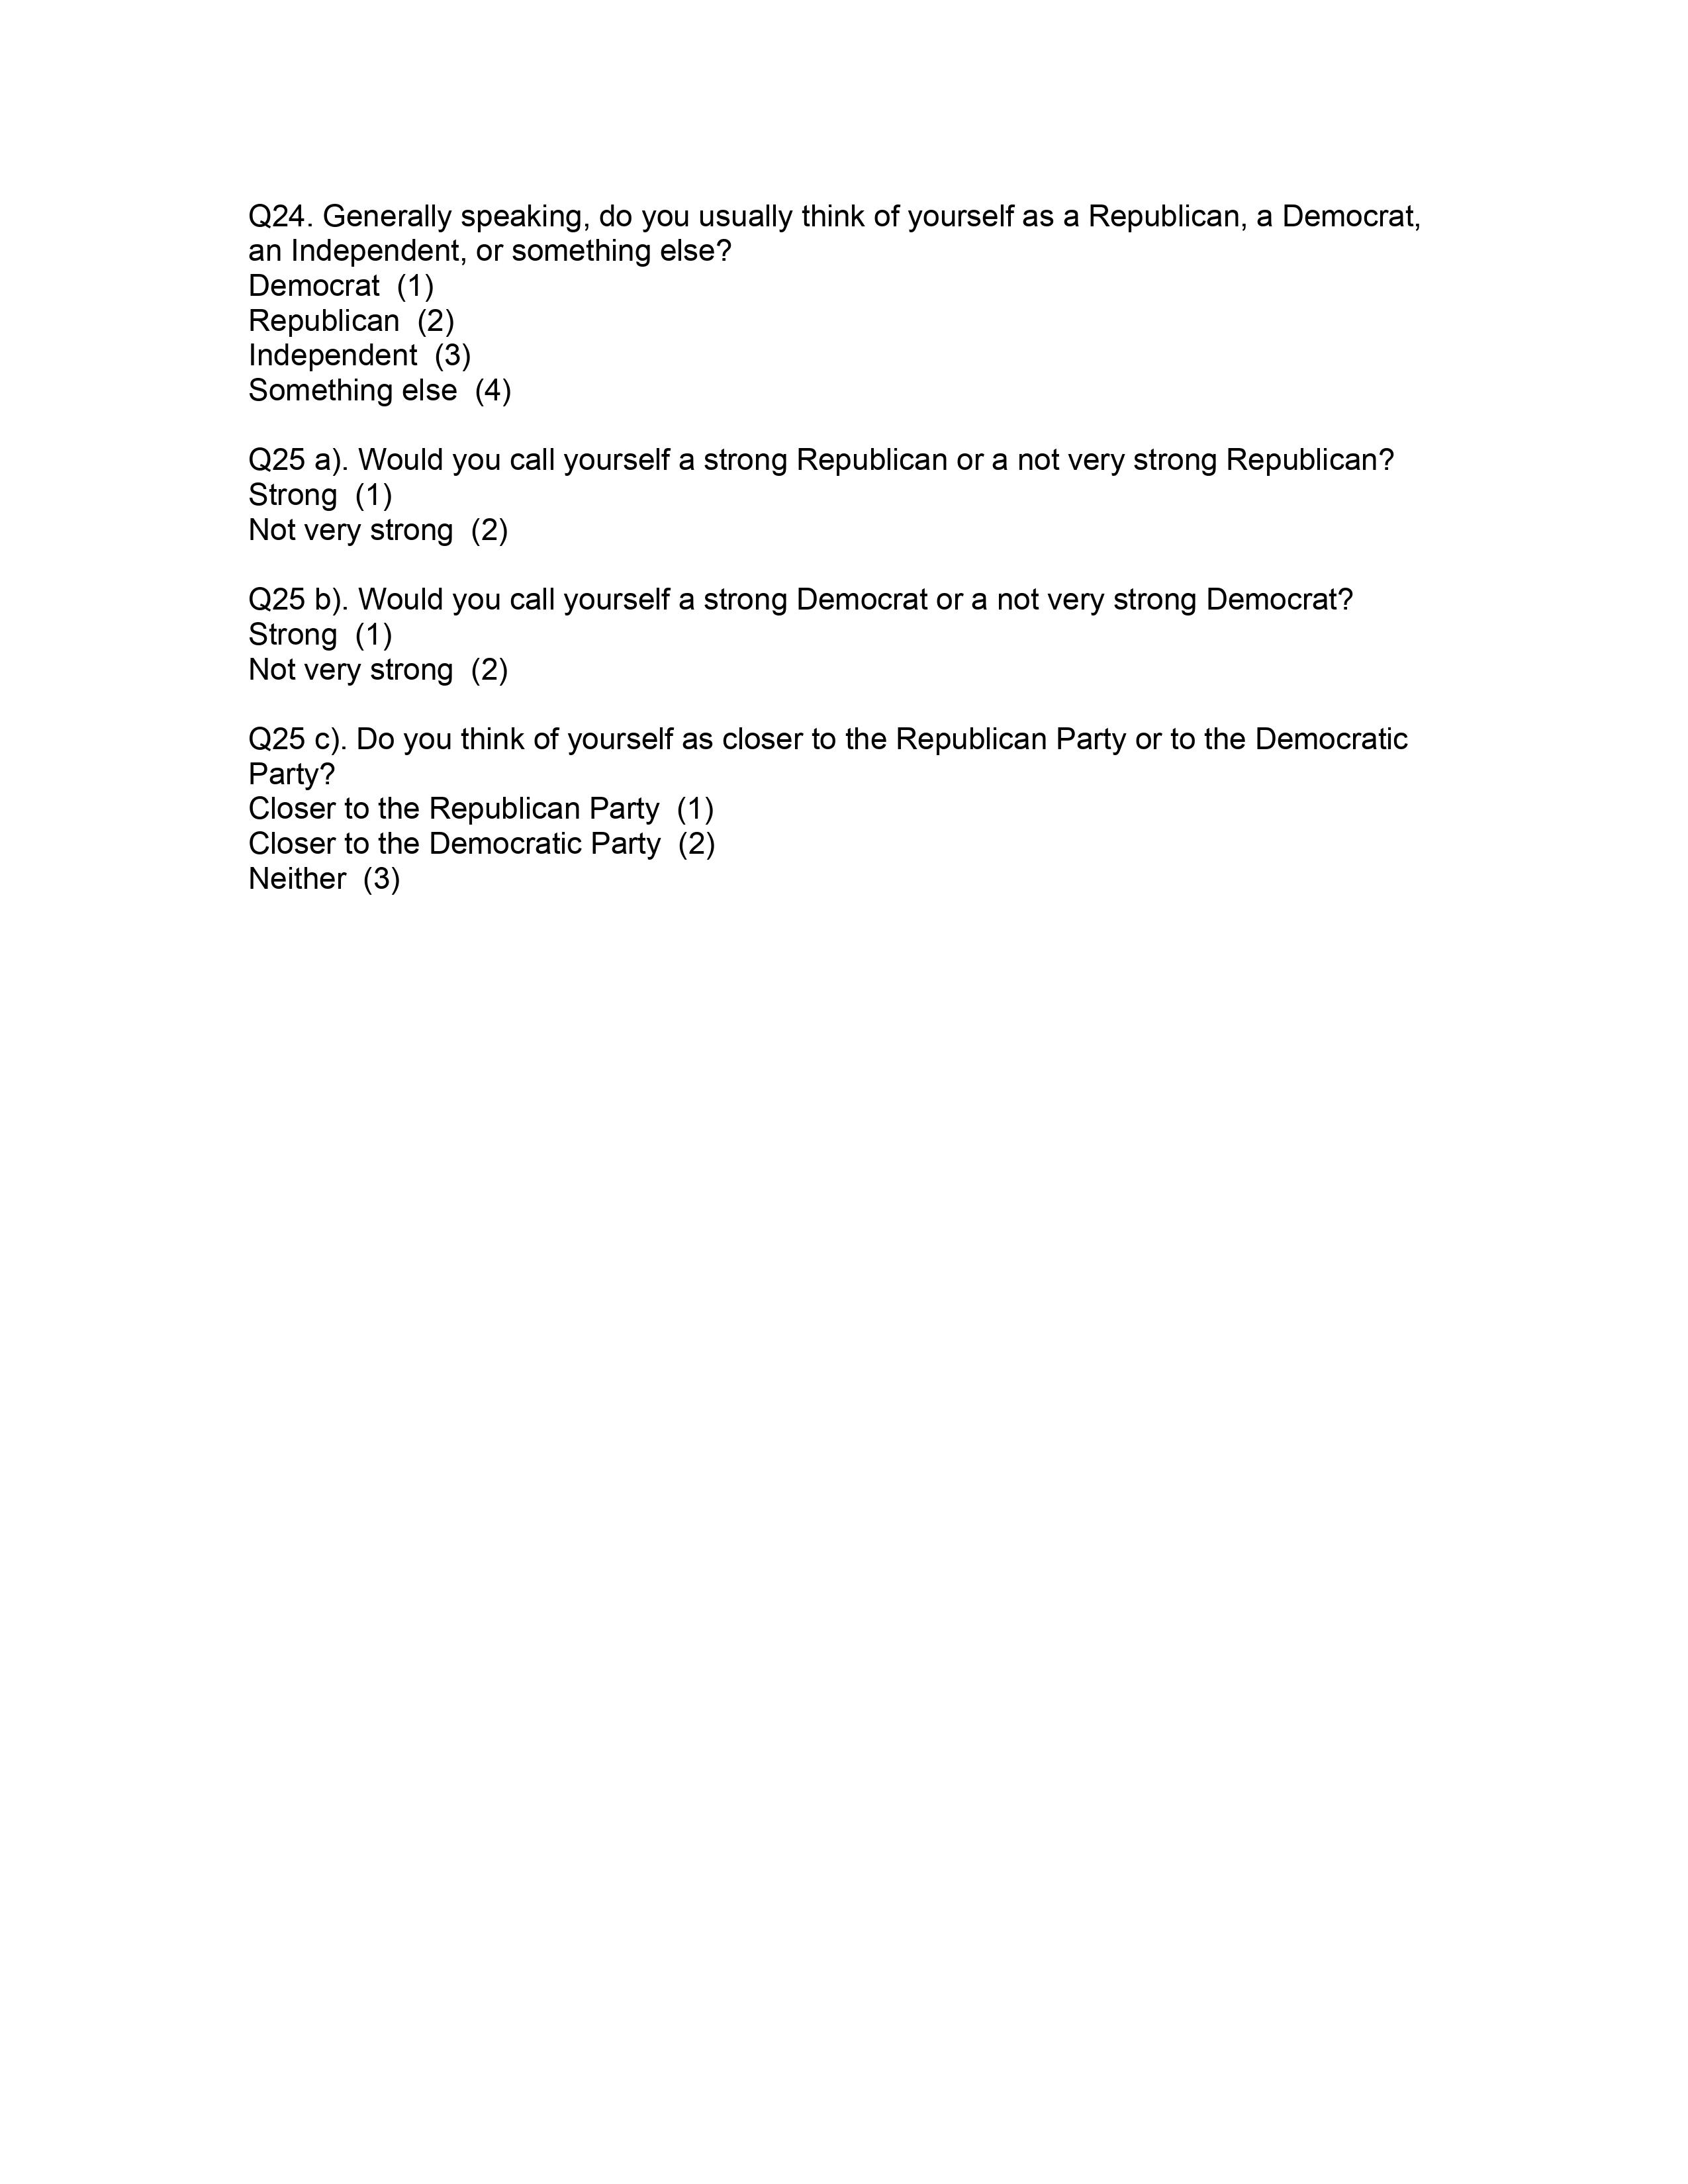
\includegraphics{data/framing/appendix/questionnaire/questionnaire12.jpg}
\end{figure}
\begin{figure}[hbt]
  \centering
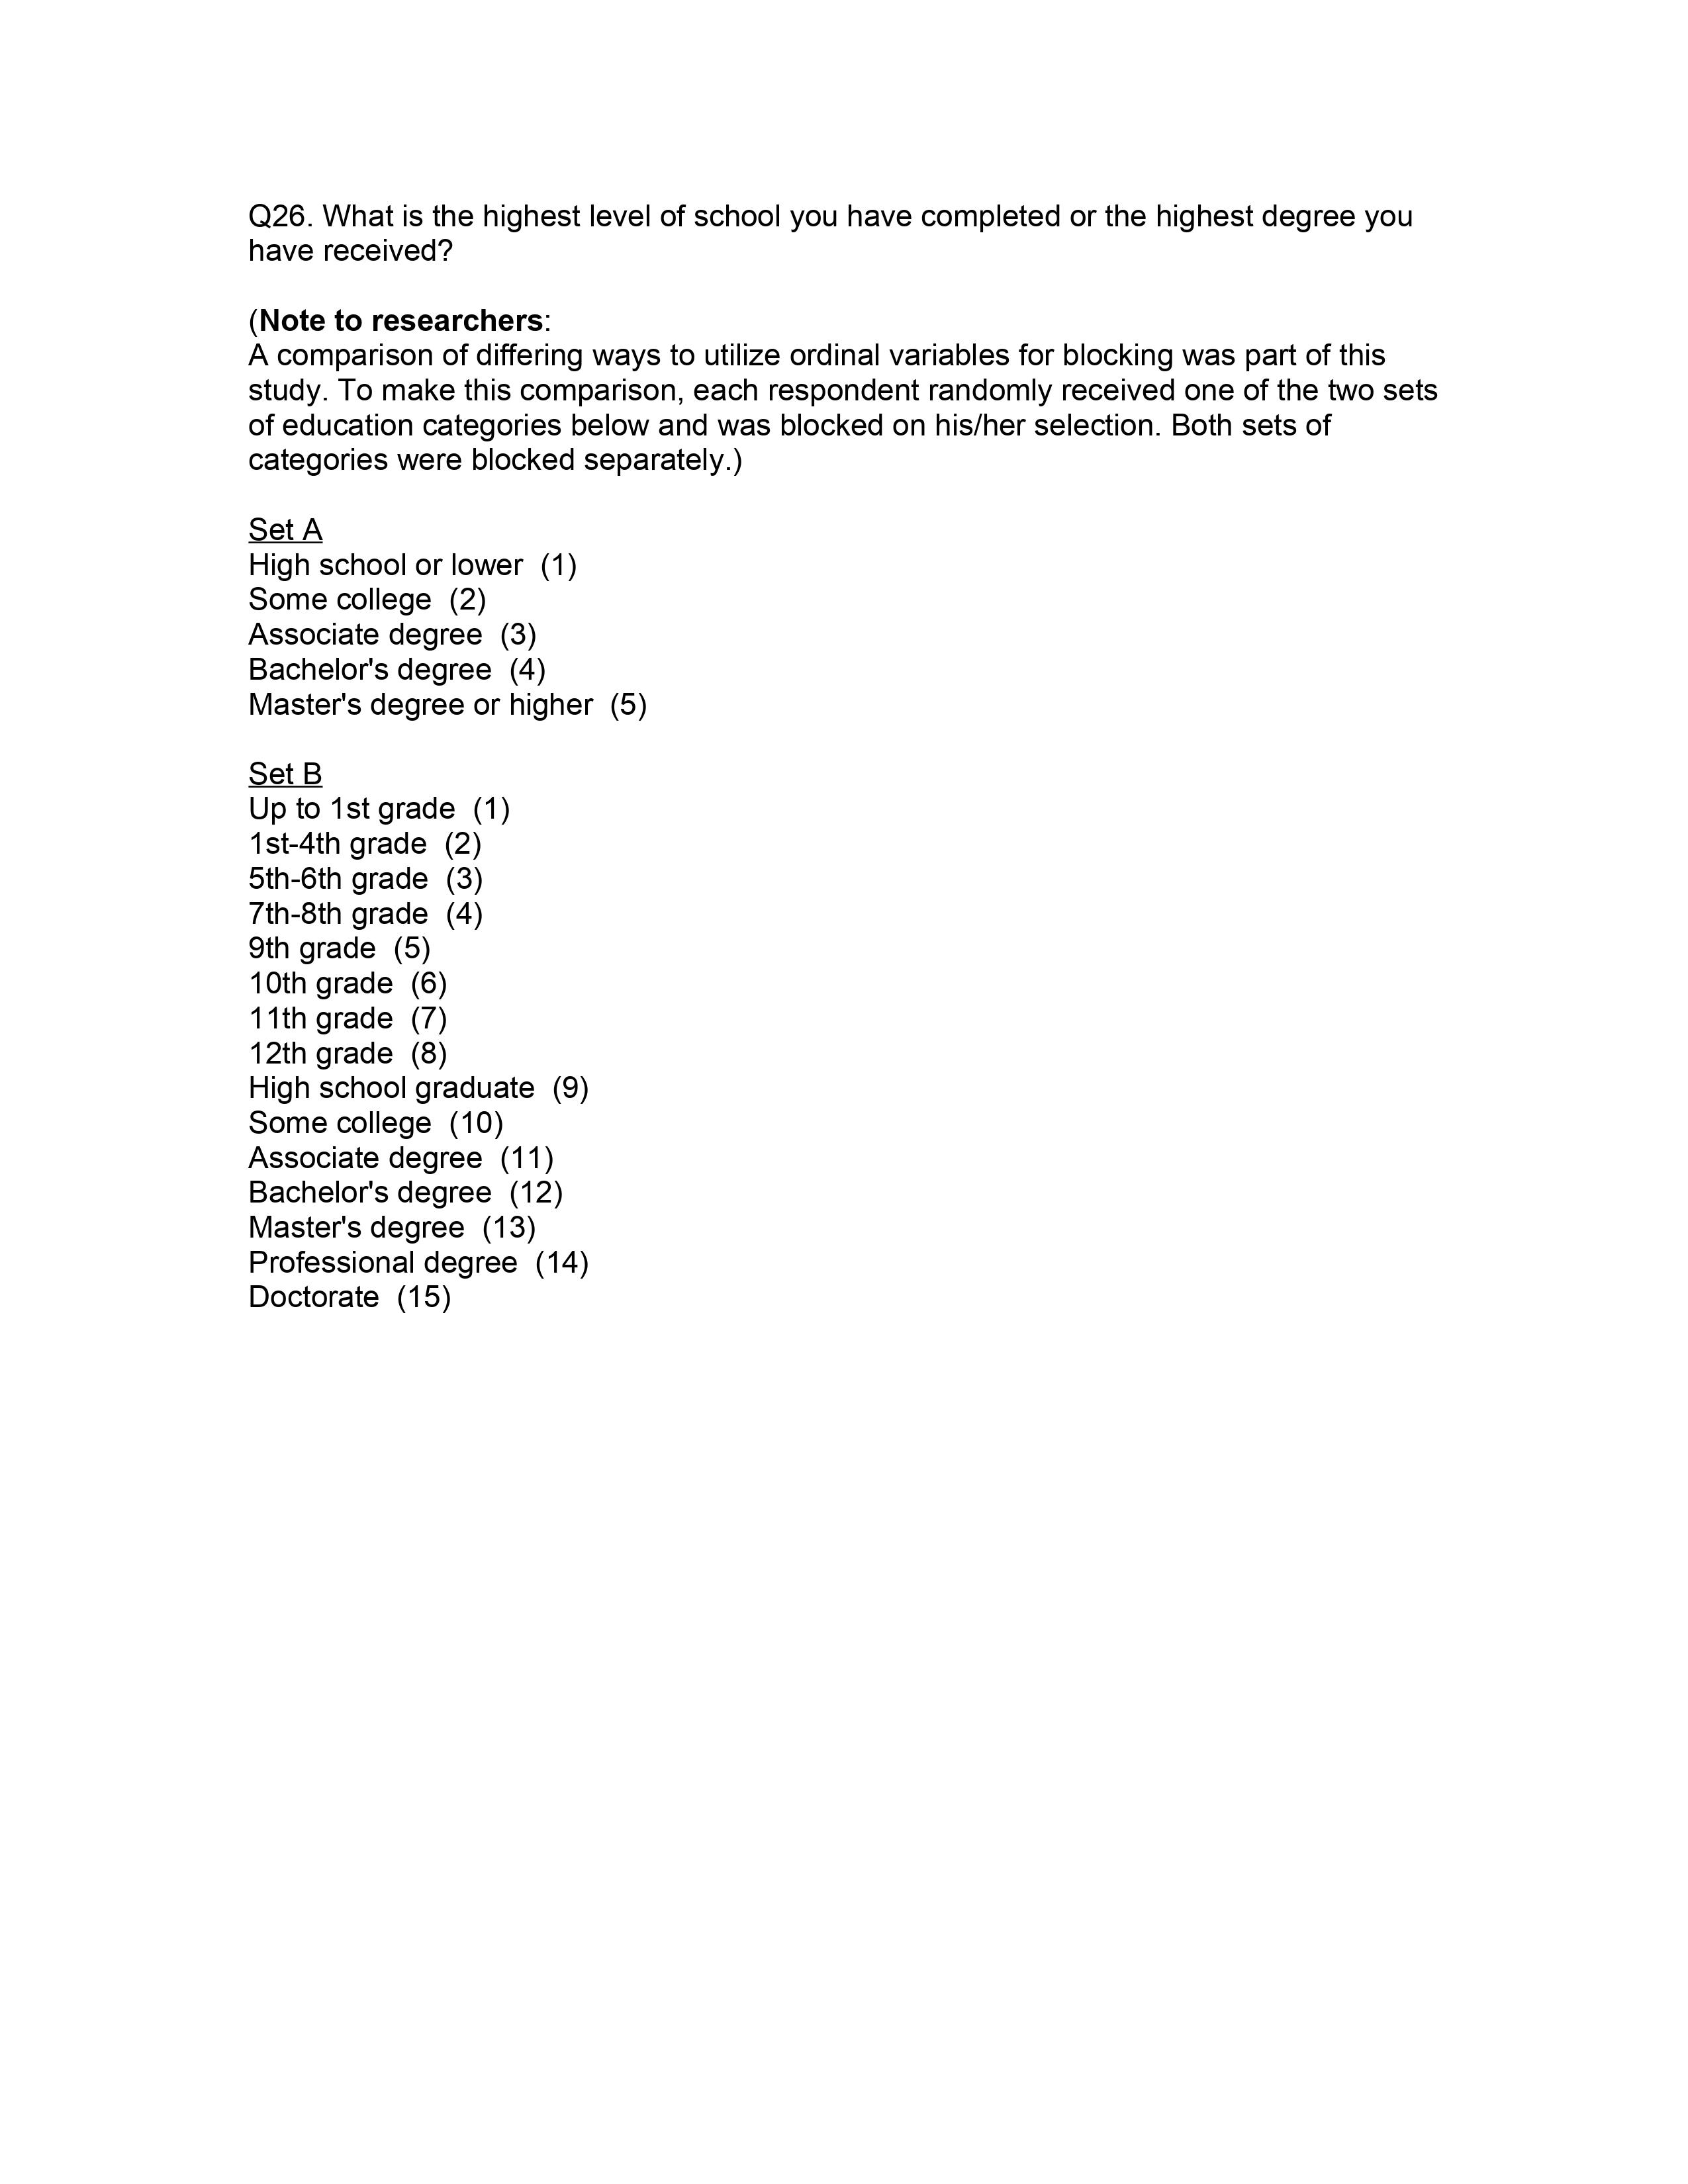
\includegraphics{data/framing/appendix/questionnaire/questionnaire13.jpg}
\end{figure}
\begin{figure}[hbt]
  \centering

\includegraphics{data/framing/appendix/questionnaire/questionnaire14.jpg}
\end{figure}
\begin{figure}[hbt]
  \centering

\includegraphics{data/framing/appendix/questionnaire/questionnaire15.jpg}
\end{figure}
\begin{figure}[hbt]
  \centering

\includegraphics{data/framing/appendix/questionnaire/questionnaire16.jpg}
\end{figure}
\begin{figure}[hbt]
  \centering

\includegraphics{data/framing/appendix/questionnaire/questionnaire17.jpg}
\end{figure}
\begin{figure}[hbt]
  \centering

\includegraphics{data/framing/appendix/questionnaire/questionnaire18.jpg}
\end{figure}
\begin{figure}[hbt]
  \centering

\includegraphics{data/framing/appendix/questionnaire/questionnaire19.jpg}
\end{figure}
\begin{figure}[hbt]
  \centering

\includegraphics{data/framing/appendix/questionnaire/questionnaire20.jpg}
\end{figure}
\begin{figure}[hbt]
  \centering

\includegraphics{data/framing/appendix/questionnaire/questionnaire21.jpg}
\end{figure}
\begin{figure}[hbt]
  \centering

\includegraphics{data/framing/appendix/questionnaire/questionnaire22.jpg}
\end{figure}
\clearpage

\hypertarget{app-framing-pid}{%
\section{Survey Experiment Results Differentiated by Party ID}\label{app-framing-pid}}

Tables \ref{exp-anes-op-rep} and \ref{exp-anes-op-dem} show the ordinal regression results differentiated by party ID. The \texttt{Moral\ Opposing} frames are stronger than the \texttt{Self-Interest\ Opposing} frames for Democrat ANES environment, Democrat OP environment, Democrat OP healthcare, and Republican ANES environment. Note that these results change, though, for Republican healthcare. Both the ANES and the OP \texttt{Self-Interest\ Opposing} frames move respondents more than their \texttt{Moral\ Opposing} counterparts. It thus appears that Republicans value self-interest more than morality when it comes to opposition to healthcare. As in the overall analysis above, the \texttt{Moral\ Supporting} frames do not move people more than the \texttt{Self-Interest\ Supporting} frames. All coefficients here include the null, with the exception of Democrat OP environment which actually shows a negative coefficient. Almost none of the control variables show statistically significant results. While the results for opposing frames for Republican healthcare are notable, these results nonetheless overall do not change the substantive conclusions for the hypotheses.

\ssp

\footnotesize

\blandscape
\centering
\captionof{table}{Ordinal Logistic Regression Results, Republican\label{exp-anes-op-rep}}
\begin{tabular}{@{\extracolsep{-60pt}}lD{.}{.}{-3} D{.}{.}{-3} D{.}{.}{-3} D{.}{.}{-3} } 
\\[-1.8ex]\hline 
\hline \\[-1.8ex] 
 & \multicolumn{4}{c}{\textit{Dependent variable:}} \\ 
\cline{2-5} 
\\[-1.8ex] & \multicolumn{2}{c}{Healthcare} & \multicolumn{2}{c}{Environment} \\ 
 & \multicolumn{1}{c}{ANES} & \multicolumn{1}{c}{OP} & \multicolumn{1}{c}{ANES} & \multicolumn{1}{c}{OP} \\ 
\hline \\[-1.8ex] 
 Moral opposing & -0.261$ $(-1.013$, $0.490) & -0.732^{}$ $(-1.397$, $-0.067) & -1.009^{}$ $(-1.711$, $-0.306) & -0.088$ $(-0.706$, $0.531) \\ 
  Moral supporting & 0.131$ $(-0.586$, $0.847) & -0.471$ $(-1.130$, $0.189) & -0.304$ $(-1.034$, $0.425) & -0.190$ $(-0.832$, $0.452) \\ 
  Self-interest opposing & -0.699^{}$ $(-1.370$, $-0.028) & -0.949^{}$ $(-1.603$, $-0.296) & -0.343$ $(-1.026$, $0.340) & 0.027$ $(-0.567$, $0.622) \\ 
  Self-interest supporting & -0.302$ $(-1.005$, $0.401) & -0.325$ $(-0.948$, $0.298) & 0.063$ $(-0.591$, $0.716) & 0.258$ $(-0.360$, $0.876) \\ 
  Employed full time & 0.222$ $(-0.743$, $1.188) & -0.114$ $(-0.832$, $0.604) & -0.222$ $(-1.150$, $0.707) & 0.137$ $(-0.608$, $0.882) \\ 
  Employed part time & 0.224$ $(-0.828$, $1.276) & -0.337$ $(-1.145$, $0.472) & -0.142$ $(-1.153$, $0.869) & 0.204$ $(-0.624$, $1.032) \\ 
  Homemaker & -0.048$ $(-1.168$, $1.072) & -0.310$ $(-1.285$, $0.664) & -0.006$ $(-1.116$, $1.103) & 0.109$ $(-0.911$, $1.130) \\ 
  Retired & -0.340$ $(-1.323$, $0.643) & -0.427$ $(-1.187$, $0.334) & -0.275$ $(-1.225$, $0.675) & 0.007$ $(-0.782$, $0.796) \\ 
  Student & 1.285$ $(-0.353$, $2.922) & 0.147$ $(-0.931$, $1.225) & -0.103$ $(-1.677$, $1.472) & -0.885$ $(-2.008$, $0.239) \\ 
  Income & -0.006$ $(-0.149$, $0.137) & -0.105^{}$ $(-0.227$, $0.018) & 0.070$ $(-0.070$, $0.209) & 0.054$ $(-0.066$, $0.174) \\ 
  Male & -0.141$ $(-0.578$, $0.295) & 0.072$ $(-0.344$, $0.488) & -0.147$ $(-0.587$, $0.293) & -0.244$ $(-0.671$, $0.183) \\ 
  5th-6th grade & -2.747^{}$ $(-5.811$, $0.317) &  & 0.288$ $(-2.255$, $2.831) &  \\ 
  7th-8th grade & 0.821$ $(-2.644$, $4.286) &  & 2.312$ $(-0.990$, $5.615) &  \\ 
  9th grade & -0.274$ $(-3.679$, $3.132) &  & 1.690$ $(-1.678$, $5.058) &  \\ 
  10th grade & -15.887^{}$ $(-15.887$, $-15.887) &  & -1.034$ $(-3.888$, $1.820) &  \\ 
  11th grade & -0.750$ $(-3.064$, $1.564) &  & -0.872$ $(-3.107$, $1.364) &  \\ 
  12th grade & -0.518$ $(-3.144$, $2.109) &  & 0.513$ $(-1.981$, $3.007) &  \\ 
  High school graduate & 0.036$ $(-1.515$, $1.587) &  & 1.158^{}$ $(-0.205$, $2.521) &  \\ 
  Some college & -0.341$ $(-1.888$, $1.206) & -0.165$ $(-0.744$, $0.413) & 1.160^{}$ $(-0.207$, $2.527) & 0.352$ $(-0.240$, $0.943) \\ 
  Associate degree & -0.626$ $(-2.207$, $0.955) & -0.209$ $(-0.872$, $0.453) & 0.739$ $(-0.666$, $2.145) & -0.152$ $(-0.818$, $0.514) \\ 
  Bachelor & -0.495$ $(-2.018$, $1.029) & 0.122$ $(-0.489$, $0.733) & 1.224^{}$ $(-0.111$, $2.559) & -0.262$ $(-0.880$, $0.356) \\ 
  Master & -1.154$ $(-2.772$, $0.465) &  & 0.868$ $(-0.564$, $2.300) &  \\ 
  Professional degree & -1.146$ $(-3.198$, $0.906) &  & 0.658$ $(-1.457$, $2.772) &  \\ 
  Master or higher &  & -0.117$ $(-0.819$, $0.586) &  & -0.097$ $(-0.814$, $0.619) \\ 
 \hline \\[-1.8ex] 
Observations & \multicolumn{1}{c}{318} & \multicolumn{1}{c}{331} & \multicolumn{1}{c}{318} & \multicolumn{1}{c}{331} \\ 
\hline \\[-1.8ex] 
\end{tabular} 
\fillandplacepagenumber
\elandscape

\dsp

\normalsize

\ssp

\footnotesize

\blandscape
\centering
\captionof{table}{Ordinal Logistic Regression Results, Democrat\label{exp-anes-op-dem}}
\begin{tabular}{@{\extracolsep{-60pt}}lD{.}{.}{-3} D{.}{.}{-3} D{.}{.}{-3} D{.}{.}{-3} } 
\\[-1.8ex]\hline 
\hline \\[-1.8ex] 
 & \multicolumn{4}{c}{\textit{Dependent variable:}} \\ 
\cline{2-5} 
\\[-1.8ex] & \multicolumn{2}{c}{Healthcare} & \multicolumn{2}{c}{Environment} \\ 
 & \multicolumn{1}{c}{ANES} & \multicolumn{1}{c}{OP} & \multicolumn{1}{c}{ANES} & \multicolumn{1}{c}{OP} \\ 
\hline \\[-1.8ex] 
 Moral opposing & -0.304$ $(-0.890$, $0.283) & -0.781^{}$ $(-1.363$, $-0.199) & -0.676^{}$ $(-1.317$, $-0.036) & -0.671^{}$ $(-1.225$, $-0.116) \\ 
  Moral supporting & 0.415$ $(-0.167$, $0.997) & -0.310$ $(-0.871$, $0.252) & -0.110$ $(-0.733$, $0.514) & -0.591^{}$ $(-1.159$, $-0.022) \\ 
  Self-interest opposing & -0.042$ $(-0.574$, $0.490) & -0.136$ $(-0.712$, $0.440) & -0.145$ $(-0.763$, $0.474) & -0.513^{}$ $(-1.081$, $0.054) \\ 
  Self-interest supporting & -0.073$ $(-0.664$, $0.517) & -0.135$ $(-0.688$, $0.419) & 0.497^{}$ $(-0.085$, $1.079) & -0.559^{}$ $(-1.138$, $0.019) \\ 
  Employed full time & 0.010$ $(-0.634$, $0.653) & -0.027$ $(-0.641$, $0.586) & -0.296$ $(-0.950$, $0.358) & 0.229$ $(-0.378$, $0.835) \\ 
  Employed part time & 0.113$ $(-0.586$, $0.813) & -0.079$ $(-0.748$, $0.591) & -0.403$ $(-1.115$, $0.309) & -0.027$ $(-0.690$, $0.636) \\ 
  Homemaker & 0.469$ $(-0.552$, $1.490) & 0.132$ $(-0.808$, $1.072) & 0.271$ $(-0.772$, $1.315) & -0.199$ $(-1.110$, $0.711) \\ 
  Retired & 0.171$ $(-0.497$, $0.839) & 0.505$ $(-0.158$, $1.169) & 0.085$ $(-0.584$, $0.754) & 0.895^{}$ $0.234$, $1.557) \\ 
  Student & -0.257$ $(-1.303$, $0.789) & -0.288$ $(-1.237$, $0.662) & -0.838$ $(-1.926$, $0.250) & 0.510$ $(-0.458$, $1.479) \\ 
  Income & -0.026$ $(-0.138$, $0.085) & -0.052$ $(-0.166$, $0.061) & -0.024$ $(-0.139$, $0.091) & 0.049$ $(-0.064$, $0.162) \\ 
  Male & 0.006$ $(-0.380$, $0.392) & 0.092$ $(-0.282$, $0.465) & -0.108$ $(-0.491$, $0.275) & -0.175$ $(-0.551$, $0.200) \\ 
  1st-4th grade & 19.675^{}$ $(17.269$, $22.080) &  & 0.217$ $(-4.350$, $4.785) &  \\ 
  7th-8th grade & 0.525^{}$ $0.525$, $0.525) &  & -15.604^{}$ $(-15.604$, $-15.604) &  \\ 
  9th grade & 21.793^{}$ $(19.747$, $23.839) &  & -1.359$ $(-6.089$, $3.371) &  \\ 
  10th grade & 24.851^{}$ $(22.655$, $27.048) &  & 2.036$ $(-2.670$, $6.741) &  \\ 
  11th grade & 23.857^{}$ $(21.309$, $26.404) &  & 0.149$ $(-4.363$, $4.660) &  \\ 
  12th grade & 22.521^{}$ $(20.929$, $24.114) &  & 0.791$ $(-3.562$, $5.144) &  \\ 
  High school graduate & 22.797^{}$ $(22.182$, $23.412) &  & 0.546$ $(-3.447$, $4.538) &  \\ 
  Some college & 23.051^{}$ $(22.499$, $23.603) & 0.566^{}$ $0.004$, $1.129) & 1.217$ $(-2.767$, $5.201) & 0.207$ $(-0.350$, $0.764) \\ 
  Associate degree & 23.238^{}$ $(22.583$, $23.894) & 0.402$ $(-0.231$, $1.034) & 1.483$ $(-2.517$, $5.483) & 0.365$ $(-0.280$, $1.009) \\ 
  Bachelor & 23.384^{}$ $(22.841$, $23.926) & 0.213$ $(-0.334$, $0.760) & 1.745$ $(-2.226$, $5.717) & 0.019$ $(-0.547$, $0.585) \\ 
  Master & 23.704^{}$ $(23.067$, $24.342) &  & 1.784$ $(-2.196$, $5.764) &  \\ 
  Professional degree & 23.191^{}$ $(22.116$, $24.265) &  & 1.935$ $(-2.144$, $6.015) &  \\ 
  Doctorate & 23.703^{}$ $(22.721$, $24.685) &  & 1.418$ $(-2.668$, $5.504) &  \\ 
  Master or higher &  & 0.694^{}$ $0.060$, $1.328) &  & -0.058$ $(-0.677$, $0.562) \\ 
 \hline \\[-1.8ex] 
Observations & \multicolumn{1}{c}{412} & \multicolumn{1}{c}{422} & \multicolumn{1}{c}{412} & \multicolumn{1}{c}{422} \\ 
\hline \\[-1.8ex] 
\end{tabular} 
\fillandplacepagenumber
\elandscape

\dsp

\normalsize

\hypertarget{app-framing-10var}{%
\section{Imputing 10 Variables with Missing Data}\label{app-framing-10var}}

Table \ref{mar.10var.frame} shows the imputation results for missing data inserted at random for 10 variables. In addition to the 5 variables in Table \ref{mar.10var.frame}, missing data is also inserted for \texttt{Student}, \texttt{Conservative}, \texttt{Black}, \texttt{Hispanic}, and \texttt{Asian}. All of these are binary variables. The results are virtually identical for all methods for \texttt{Democrat}, \texttt{Male}, \texttt{Student}, \texttt{Conservative}, \texttt{Black}, \texttt{Hispanic}, \texttt{Asian} for both data sets. The only exception among the binary variables is \texttt{Employed}, where \texttt{hd.ord} and \texttt{hot.deck} perform worse than \texttt{mice} and \texttt{amelia}. The results for \texttt{Income} and \texttt{Age} repeat the pattern from Table \ref{mar.5var.frame}: \texttt{amelia} overall beats \texttt{mice}, the hot decking methods show a much larger distance, and \texttt{hd.ord} performs worst out of all methods. Notably, \texttt{na.omit} produces better results than the hot decking methods for \texttt{Age} for both data sets.

\ssp

\footnotesize
\begin{longtable}{ccr@{}lr@{}l} 
 \caption{Accuracy of Multiple Imputation Methods. Framing Data, MAR, 10 Variables with NA}   
 \label{mar.10var.frame}  
 \\[-1.8ex]\hline
 \hline \\[-1.8ex] 
\multicolumn{1}{c}{Method} & \multicolumn{1}{c}{Variable} & \multicolumn{2}{c}{ANES} & \multicolumn{2}{c}{OP} \\ 
 \hline \\[-1.8ex] 
 true & Democrat & 0.&3879 & 0.&3826 \\ 
 hot.deck & Democrat & + 0.&0003 & + 0.&0003 \\ 
 hd.ord & Democrat & + 0.&0002 & + 0.&0003 \\
 amelia & Democrat & + 0.&0002 & + 0.&0000 \\
 mice & Democrat & + 0.&0001 & --0.&0001 \\
 na.omit & Democrat & --0.&0217 & --0.&0249 \\
 true & Male & 0.&4576 & 0.&4714 \\ 
 hot.deck & Male & --0.&0001 & + 0.&0003 \\
 hd.ord & Male & + 0.&0000 & + 0.&0002 \\
 amelia & Male & + 0.&0001 & + 0.&0000 \\ 
 mice & Male & + 0.&0000 & --0.&0001 \\  
 na.omit & Male & --0.&0334 & --0.&0325 \\ 
 true & Employed & 0.&5612 & 0.&5684 \\ 
 hot.deck & Employed & + 0.&0013 & + 0.&0013 \\
 hd.ord & Employed & + 0.&0013 & + 0.&0014 \\ 
 amelia & Employed & + 0.&0002 & + 0.&0001 \\
 mice & Employed & + 0.&0000 & + 0.&0000 \\ 
 na.omit & Employed & --0.&0277 & --0.&0260 \\
 true & Income & 3.&5537 & 3.&4923 \\  
 hot.deck & Income & --0.&0037 & --0.&0035 \\ 
 hd.ord & Income & --0.&0081 & --0.&0074 \\ 
 amelia & Income & + 0.&0000 & --0.&0001 \\
 mice & Income & --0.&0001 & --0.&0002 \\  
 na.omit & Income & --0.&1501 & --0.&1504 \\ 
 true & Age & 46.&3475 & 44.&9574 \\ 
 hot.deck & Age & --0.&1106 & --0.&1115 \\ 
 hd.ord & Age & --0.&1632 & --0.&1593 \\
 amelia & Age & --0.&0019 & + 0.&0008 \\ 
 mice & Age & --0.&0068 & --0.&0009 \\ 
 na.omit & Age & --0.&0890 & --0.&0921 \\ 
 true & Student & 0.&0386 & 0.&0481 \\ 
 hot.deck & Student & --0.&0001 & + 0.&0000 \\
 hd.ord & Student & + 0.&0000 & + 0.&0001 \\
 amelia & Student & + 0.&0001 & + 0.&0000 \\
 mice & Student & + 0.&0000 & --0.&0001 \\
 na.omit & Student & --0.&0069 & --0.&0065 \\ 
 true & Conservative & 0.&3908 & 0.&3744 \\ 
 hot.deck & Conservative & + 0.&0001 & + 0.&0004 \\
 hd.ord & Conservative & --0.&0002 & + 0.&0003 \\ 
 amelia & Conservative & + 0.&0000 & + 0.&0001 \\ 
 mice & Conservative & --0.&0002 & + 0.&0002 \\
 na.omit & Conservative & --0.&0177 & --0.&0193 \\
 true & Black & 0.&1158 & 0.&1242 \\ 
 hot.deck & Black & + 0.&0004 & + 0.&0003 \\ 
 hd.ord & Black & + 0.&0005 & + 0.&0004 \\ 
 amelia & Black & + 0.&0000 & + 0.&0000 \\ 
 mice & Black & + 0.&0001 & + 0.&0000 \\
 na.omit & Black & --0.&0094 & --0.&0086 \\
 true & Democrat & 0.&0895 & 0.&0907 \\ 
 hot.deck & Democrat & + 0.&0004 & + 0.&0003 \\ 
 hd.ord & Democrat & + 0.&0003 & + 0.&0001 \\ 
 amelia & Democrat & + 0.&0000 & + 0.&0000 \\
 mice & Democrat & --0.&0001 & + 0.&0000 \\
 na.omit & Democrat & --0.&0126 & --0.&0152 \\ 
 true & Asian & 0.&0810 & 0.&0662 \\
 hot.deck & Asian & + 0.&0001 & --0.&0002 \\ 
 hd.ord & Asian & + 0.&0000 & --0.&0001 \\
 amelia & Asian & + 0.&0001 & + 0.&0000 \\
 mice & Asian & + 0.&0000 & + 0.&0000 \\ 
 na.omit & Asian & --0.&0165 & --0.&0142 \\ 
 \hline \\[-1.8ex]
 \end{longtable}
\dsp

\normalsize

As was the case for Tables \ref{mar.5var.frame} and \ref{mnar.5var.frame}, all imputation results for missing data inserted not at random for 10 variables (Table \ref{mnar.10var.frame}) are much further away from the true values than in Table \ref{mar.10var.frame}. There are still several binary variables where all methods produce virtually identical results (\texttt{Democrat}, \texttt{Male}, \texttt{Employed}, \texttt{Conservative}), but distances between \texttt{hd.ord} and \texttt{mice}/\texttt{amelia} are notably larger for \texttt{Student}, \texttt{Black}, \texttt{Hispanic}, and \texttt{Asian}. Similarly to before, the distances between \texttt{hd.ord} and \texttt{mice}/\texttt{amelia} decrease for \texttt{Income} and \texttt{Age} when compared to the results for 10 variables MAR. \texttt{hd.ord} once again performs worst for both interval variables for both data sets. Note that \texttt{na.omit} is now overall much closer to the imputation methods and the true values. It even produces the best results for \texttt{Age} across all methods for both data sets.

\ssp

\footnotesize
\begin{longtable}{ccr@{}lr@{}l} 
 \caption{Accuracy of Multiple Imputation Methods. Framing Data, MNAR, 10 Variables with NA}   
 \label{mnar.10var.frame}
 \\[-1.8ex]\hline
 \hline \\[-1.8ex]
\multicolumn{1}{c}{Method} & \multicolumn{1}{c}{Variable} & \multicolumn{2}{c}{ANES} & \multicolumn{2}{c}{OP} \\ 
 \hline \\[-1.8ex]  
 true & Democrat & 0.&3879 & 0.&3826 \\
 hot.deck & Democrat & --0.&0015 & --0.&0016 \\
 hd.ord & Democrat & --0.&0019 & --0.&0019 \\
 amelia & Democrat & --0.&0015 & --0.&0015 \\
 mice & Democrat & --0.&0013 & --0.&0014 \\ 
 na.omit & Democrat & --0.&0084 & --0.&0094 \\ 
 true & Male & 0.&4576 & 0.&4714 \\
 hot.deck & Male & --0.&0067 & --0.&0063 \\ 
 hd.ord & Male & --0.&0066 & --0.&0062 \\ 
 amelia & Male & --0.&0066 & --0.&0065 \\
 mice & Male & --0.&0067 & --0.&0066 \\
 na.omit & Male & --0.&0102 & --0.&0099 \\ 
 true & Employed & 0.&5612 & 0.&5684 \\ 
 hot.deck & Employed & --0.&0013 & --0.&0015 \\ 
 hd.ord & Employed & --0.&0014 & --0.&0017 \\
 amelia & Employed & --0.&0015 & --0.&0015 \\ 
 mice & Employed & --0.&0015 & --0.&0015 \\
 na.omit & Employed & --0.&0086 & --0.&0077 \\
 true & Income & 3.&5537 & 3.&4923 \\
 hot.deck & Income & --0.&0241 & --0.&0237 \\ 
 hd.ord & Income & --0.&0262 & --0.&0267 \\
 amelia & Income & --0.&0196 & --0.&0212 \\
 mice & Income & --0.&0196 & --0.&0214 \\ 
 na.omit & Income & --0.&0476 & --0.&0490 \\
 true & Age & 46.&3475 & 44.&9574 \\
 hot.deck & Age & --0.&2197 & --0.&2388 \\
 hd.ord & Age & --0.&3100 & --0.&2911 \\ 
 amelia & Age & --0.&1196 & --0.&1307 \\ 
 mice & Age & --0.&1207 & --0.&1341 \\ 
 na.omit & Age & --0.&0274 & --0.&0193 \\ 
 true & Student & 0.&0386 & 0.&0481 \\ 
 hot.deck & Student & --0.&0022 & --0.&0024 \\
 hd.ord & Student & --0.&0023 & --0.&0025 \\
 amelia & Student & --0.&0020 & --0.&0024 \\
 mice & Student & --0.&0015 & --0.&0018 \\
 na.omit & Student & --0.&0026 & --0.&0032 \\
 true & Conservative & 0.&3908 & 0.&3744 \\
 hot.deck & Conservative & --0.&0043 & --0.&0038 \\
 hd.ord & Conservative & --0.&0045 & --0.&0041 \\
 amelia & Conservative & --0.&0042 & --0.&0045 \\ 
 mice & Conservative & --0.&0044 & --0.&0043 \\
 na.omit & Conservative & --0.&0059 & --0.&0065 \\
 true & Black & 0.&1158 & 0.&1242 \\
 hot.deck & Black & --0.&0032 & --0.&0030 \\
 hd.ord & Black & --0.&0033 & --0.&0030 \\
 amelia & Black & --0.&0023 & --0.&0021 \\
 mice & Black & --0.&0023 & --0.&0020 \\ 
 na.omit & Black & --0.&0049 & --0.&0050 \\ 
 true & Democrat & 0.&0895 & 0.&0907 \\ 
 hot.deck & Democrat & --0.&0027 & --0.&0028 \\
 hd.ord & Democrat & --0.&0034 & --0.&0036 \\
 amelia & Democrat & --0.&0023 & --0.&0022 \\
 mice & Democrat & --0.&0023 & --0.&0021 \\ 
 na.omit & Democrat & --0.&0050 & --0.&0057 \\ 
 true & Asian & 0.&0810 & 0.&0662 \\ 
 hot.deck & Asian & --0.&0034 & --0.&0031 \\ 
 hd.ord & Asian & --0.&0038 & --0.&0032 \\ 
 amelia & Asian & --0.&0023 & --0.&0020 \\
 mice & Asian & --0.&0025 & --0.&0017 \\
 na.omit & Asian & --0.&0059 & --0.&0046 \\ 
 \hline \\[-1.8ex] 
 \end{longtable}
\dsp

\normalsize

\hypertarget{references}{%
\chapter*{REFERENCES}\label{references}}
\addcontentsline{toc}{chapter}{REFERENCES}

\noindent

\ssp

\hypertarget{refs}{}
\leavevmode\hypertarget{ref-aaroe_investigating_2011}{}%
Aaroe, L. (2011). Investigating Frame Strength: The Case of Episodic and Thematic Frames. \emph{Political Communication}, \emph{28}(2), 207--226.

\leavevmode\hypertarget{ref-abramowitz_1995_abortion}{}%
Abramowitz, A. I. (1995). It's Abortion, Stupid: Policy Voting in the 1992 Presidential Election. \emph{The Journal of Politics}, \emph{57}(1), 176--186.

\leavevmode\hypertarget{ref-abramowitz_disappearing_2010}{}%
Abramowitz, A. I. (2010). \emph{The Disappearing Center: Engaged Citizens, Polarization, and American Democracy}. New Haven, CT: Yale University Press.

\leavevmode\hypertarget{ref-acharya_2016_explaining}{}%
Acharya, A., Blackwell, M., \& Sen, M. (2016). Explaining Causal Findings without Bias: Detecting and Assessing Direct Effects. \emph{American Political Science Review}, \emph{110}(3), 512--529.

\leavevmode\hypertarget{ref-agresti_1990_categorical}{}%
Agresti, A. (1990). \emph{Categorical data analysis}. Hoboken, NJ: Wiley-Interscience.

\leavevmode\hypertarget{ref-agresti_1996_introduction}{}%
Agresti, A. (1996). \emph{An Introduction to Categorical Data Analysis}. Hoboken, NJ: Wiley-Interscience.

\leavevmode\hypertarget{ref-agresti_2010_analysis}{}%
Agresti, A. (2010). \emph{Analysis of ordinal categorical data} (2nd ed.). Hoboken, NJ: Wiley-Interscience.

\leavevmode\hypertarget{ref-allison_2002_missing}{}%
Allison, P. D. (2002). \emph{Missing Data}. Thousand Oaks, CA: SAGE Publications.

\leavevmode\hypertarget{ref-andridge_2010_review}{}%
Andridge, R. R., \& Little, R. J. (2010). A Review of Hot Deck Imputation for Survey Non-Response. \emph{International Statistical Review}, \emph{78}(1), 40--64.

\leavevmode\hypertarget{ref-andsager_how_2000}{}%
Andsager, J. (2000). How Interest Groups Attempt to Shape Public Opinion with Competing News Frames. \emph{Journalism and Mass Communication Quarterly}, \emph{77}(3), 577--592.

\leavevmode\hypertarget{ref-anduiza_2016_answering}{}%
Anduiza, E., \& Galais, C. (2016). Answering without Reading: IMCs and Strong Satisficing in Online Surveys. \emph{International Journal of Public Opinion Research}, \emph{29}(3), 497--519.

\leavevmode\hypertarget{ref-arceneaux_cognitive_2012}{}%
Arceneaux, K. (2012). Cognitive Biases and the Strength of Political Arguments. \emph{American Journal of Political Science}, \emph{56}(2), 271--285.

\leavevmode\hypertarget{ref-aronow_2019_note}{}%
Aronow, P., Baron, J., \& Pinson, L. (2019). A Note on Dropping Experimental Subjects Who Fail a Manipulation Check. \emph{Political Analysis}, \emph{27}(4), 572--589.

\leavevmode\hypertarget{ref-arrow_1967_values}{}%
Arrow, K. J. (1967). Values and Collective Decision-Making. In P. Laslett \& W. G. Runciman (Eds.), \emph{Philosophy, Politics, and Society} (pp. 215--232). New York, NY: Basic Books.

\leavevmode\hypertarget{ref-bailar_1997_comparison}{}%
Bailar, J. C., \& Bailar, B. A. (1997). Comparison of the Biases of the ``Hot Deck'' Imputation Procedure with an ``Equal Weights'' Imputation Procedure. \emph{Symposium on Incomplete Data: Panel on Incomplete Data of the Committee on National Statistics, National Research Council}, 422--447.

\leavevmode\hypertarget{ref-baldwin_1990_politics}{}%
Baldwin, P. (1990). \emph{The Politics of Social Solidarity: Class Bases of the European Welfare State, 1875--1975}. Cambridge, MA: Cambridge University Press.

\leavevmode\hypertarget{ref-barari_2017_package}{}%
Barari, S., Berwick, E., Hainmueller, J., Hopkins, D. J., Liu, S., Strezhnev, A., \& Yamamoto, T. (2017). Package ``cjoint''. Retrieved from \url{https://cran.r-project.org/web/packages/cjoint/cjoint.pdf}

\leavevmode\hypertarget{ref-bartels_2003_democracy}{}%
Bartels, L. (2003). Democracy with Attitudes. In M. B. MacKuen \& G. Rabinowitz (Eds.), \emph{Electoral Democracy} (pp. 48--82). Ann Arbor, MI: University of Michigan Press.

\leavevmode\hypertarget{ref-bartels_2005_homer}{}%
Bartels, L. (2005). Homer Gets a Tax Cut: Inequality and Public Policy in the American Mind. \emph{Perspectives on Politics}, \emph{3}(1), 15--31.

\leavevmode\hypertarget{ref-bartels_1999_panel}{}%
Bartels, L. M. (1999). Panel Effects in the American National Election Studies. \emph{Political Analysis}, \emph{8}(1), 1--8.

\leavevmode\hypertarget{ref-bartels_2006_whats}{}%
Bartels, L. M. (2006). What's the Matter with 'What's the Matter with Kansas'? \emph{Quarterly Journal of Political Science}, \emph{1}, 201--226.

\leavevmode\hypertarget{ref-batson_altruism_1991}{}%
Batson, C. D. (1991). \emph{The Altruism Question: Toward a Social Psychological Answer}. Hillsdale, NJ: Erlbaum.

\leavevmode\hypertarget{ref-bauman_2009_mind}{}%
Bauman, C. W., \& Skitka, L. J. (2009). In the Mind of the Perceiver: Psychological Implications of Moral Conviction. In D. M. Bartels, C. W. Bauman, L. J. Skitka, \& D. L. Medin (Eds.), \emph{The Psychology of Learning and Motivation} (Vol. 50, pp. 339--362). Cambridge, MA: Academic Press.

\leavevmode\hypertarget{ref-becker_1996_accounting}{}%
Becker, G. S. (1996). \emph{Accounting for tastes}. Cambridge, MA: Harvard University Press.

\leavevmode\hypertarget{ref-berinsky_evaluating_2012}{}%
Berinsky, A. J., Huber, G. A., \& Lenz, G. S. (2012). Evaluating Online Labor Markets for Experimental Research: Amazon.Com's Mechanical Turk. \emph{Political Analysis}, \emph{20}(3), 351--368.

\leavevmode\hypertarget{ref-berinsky_2014_separating}{}%
Berinsky, A. J., Margolis, M. F., \& Sances, M. W. (2014). Separating the Shirkers from the Workers? Making Sure Respondents Pay Attention on Self-Administered Surveys. \emph{American Journal of Political Science}, \emph{58}(3), 739--753.

\leavevmode\hypertarget{ref-bertrand_2004_much}{}%
Bertrand, M., Duflo, E., \& Mullainathan, S. (2004). How Much Should We Trust Differences-In-Differences Estimates? \emph{NBER Working Paper}, \emph{8841}.

\leavevmode\hypertarget{ref-biggers_2011_when}{}%
Biggers, D. R. (2011). When Ballot Issues Matter: Social Issue Ballot Measures and Their Impact on Turnout. \emph{Political Behavior}, \emph{33}(1), 3--25.

\leavevmode\hypertarget{ref-boas_fielding_2013}{}%
Boas, T. C., \& Hidalgo, F. D. (2013). Fielding Complex Online Surveys Using rApache and Qualtrics. \emph{The Political Methodologist}, \emph{20}(2), 21--26.

\leavevmode\hypertarget{ref-bodner_2008_what}{}%
Bodner, T. E. (2008). What Improves with Increased Missing Data Imputations? \emph{Structural Equation Modeling}, \emph{15}, 651--675.

\leavevmode\hypertarget{ref-brand_1999_development}{}%
Brand, J. P. (1999). \emph{Development, Implementation and Evaluation of Multiple Imputation Strategies for the Statistical Analysis of Incomplete Data Sets} (PhD thesis). Erasmus University, Rotterdam.

\leavevmode\hypertarget{ref-brewer_values_2005}{}%
Brewer, P., \& Gross, K. (2005). Values, Framing, and Citizens' Thoughts About Policy Issues: Effects on Content and Quantity. \emph{Political Psychology}, \emph{26}(6), 929--948.

\leavevmode\hypertarget{ref-brockner_2002_making}{}%
Brockner, J. (2002). Making Sense of Procedural Fairness: How High Procedural Fairness Can Reduce or Heighten the Influence of Outcome Favorability. \emph{The Academy of Management Review}, \emph{27}(1), 58--76.

\leavevmode\hypertarget{ref-brooks_2007_welfare}{}%
Brooks, C., \& Manza, J. (2007). \emph{Why Welfare States Persist: The Importance of Public Opinion in Democracies}. Chicago, IL: University of Chicago Press.

\leavevmode\hypertarget{ref-brown_1994_efficacy}{}%
Brown, R. L. (1994). Efficacy of the Indirect Approach for Estimating Structural Equation Models with Missing Data: A Comparison of Five Methods. \emph{Structural Equation Modeling}, \emph{1}, 287--316.

\leavevmode\hypertarget{ref-burnham_2018_mturk}{}%
Burnham, M. J., Le, Y. K., \& Piedmont, R. L. (2018). Who Is Mturk? Personal Characteristics and Sample Consistency of These Online Workers. \emph{Mental Health, Religion \& Culture}, \emph{21}(9-10), 934--944.

\leavevmode\hypertarget{ref-buss_2015_handbook}{}%
Buss, D. M. (2015). \emph{The Handbook of Evolutionary Psychology}. Hoboken, NJ: Wiley-Interscience.

\leavevmode\hypertarget{ref-buuren_2007_multiple}{}%
Buuren, S. van. (2007). Multiple Imputation of Discrete and Continuous Data by Fully Conditional Specification. \emph{Statistical Methods in Medical Research}, \emph{16}(3), 219--242.

\leavevmode\hypertarget{ref-buuren_2006_fully}{}%
Buuren, S. van, Brand, J. P., Groothuis-Oudshoorn, C., \& Rubin, D. (2006). Fully Conditional Specification in Multivariate Imputation. \emph{Journal of Statistical Computation and Simulation}, \emph{76}(12), 1049--1064.

\leavevmode\hypertarget{ref-buuren_2011_mice}{}%
Buuren, S. van, \& Groothuis-Oudshoorn, K. (2011). MICE: Multivariate Imputation by Chained Equations in R. \emph{Journal of Statistical Software}, \emph{45}(3), 1--67.

\leavevmode\hypertarget{ref-buuren_2020_package}{}%
Buuren, S. van, Groothuis-Oudshoorn, K., Vink, G., Schouten, R., Robitzsch, A., Doove, L., \ldots{} Gray, B. (2020). Package ``mice''. Retrieved from \url{https://cran.r-project.org/web/packages/mice/mice.pdf}

\leavevmode\hypertarget{ref-buuren_2000_multiple}{}%
Buuren, S. van, \& Oudshoorn, K. (2000). \emph{Multiple Imputation by Chained Equations: MICE V1.0 User's Manual}. TNO Prevention; Health, Leiden.

\leavevmode\hypertarget{ref-callaghan_introduction_2005}{}%
Callaghan, K., \& Schnell, F. (2005). Introduction: Framing Political Issues in American Politics. In K. Callaghan \& F. Schnell (Eds.), \emph{Framing American politics} (pp. 1--17). Pittsburgh, PA: University of Pittsburgh Press.

\leavevmode\hypertarget{ref-campbell_american_1960}{}%
Campbell, A., Converse, P. E., Miller, W. E., \& Stokes, D. E. (1960). \emph{The American Voter}. Chicago, IL: Chicago University Press.

\leavevmode\hypertarget{ref-carnes_2012_harm}{}%
Carnes, N., \& Janoff-Bulman, R. (2012). Harm, Help, and the Nature of (Im)Moral (In)Action. \emph{Psychological Inquiry}, \emph{23}, 137--142.

\leavevmode\hypertarget{ref-carpini_1993_measuring}{}%
Carpini, M. X. D., \& Keeter, S. (1993). Measuring political knowledge: Putting first things first. \emph{American Journal of Political Science}, \emph{37}(4), 1179--1206.

\leavevmode\hypertarget{ref-cervone_2004_architecture}{}%
Cervone, D. (2004). The Architecture of Personality. \emph{Psychological Review}, \emph{111}, 183--204.

\leavevmode\hypertarget{ref-chong_when_2001}{}%
Chong, D., Citrin, J., \& Conley, P. (2001). When Self-Interest Matters. \emph{Political Psychology}, \emph{22}(3), 541--557.

\leavevmode\hypertarget{ref-chong_framing_2007}{}%
Chong, D., \& Druckman, J. N. (2007). Framing Public Opinion in Competitive Democracies. \emph{American Political Science Review}, \emph{101}(4), 637--655.

\leavevmode\hypertarget{ref-chong_dynamic_2010}{}%
Chong, D., \& Druckman, J. N. (2010). Dynamic Public Opinion: Communication Effects Over Time. \emph{American Political Science Review}, \emph{104}(4), 663--680.

\leavevmode\hypertarget{ref-chong_counterframing_2013}{}%
Chong, D., \& Druckman, J. N. (2013). Counterframing Effects. \emph{Journal of Politics}, \emph{75}(1), 1--16.

\leavevmode\hypertarget{ref-chow_2007_adaptive}{}%
Chow, S.-C., \& Chang, M. (2007). \emph{Adaptive design methods in clinical trials}. Boca Raton, FL: Chapman; Hall.

\leavevmode\hypertarget{ref-citrin_1990_self-interest}{}%
Citrin, J., \& Green, D. P. (1990). The Self-Interest Motive in American Public Opinion. \emph{Research in Micropolitics}, \emph{3}, 1--28.

\leavevmode\hypertarget{ref-clifford_2015_moral}{}%
Clifford, S., Iyengar, V., Cabeza, R., \& Sinnott-Armstrong, W. (2015a). Moral Foundations Vignettes: A Standardized Stimulus Database of Scenarios Based on Moral Foundations Theory. \emph{Behavior Research Methods}, \emph{47}, 1178--1198.

\leavevmode\hypertarget{ref-clifford_2013_words}{}%
Clifford, S., \& Jerit, J. (2013). How Words Do the Work of Politics: Moral Foundations Theory and the Debate over Stem Cell Research. \emph{The Journal of Politics}, \emph{75}(3), 659--671.

\leavevmode\hypertarget{ref-clifford_2014_there}{}%
Clifford, S., \& Jerit, J. (2014). Is There a Cost to Convenience? An Experimental Comparison of Data Quality in Laboratory and Online Studies. \emph{Journal of Experimental Political Science}, \emph{1}(2), 120--131.

\leavevmode\hypertarget{ref-clifford_2015_samples}{}%
Clifford, S., Jewell, R. M., \& Waggoner, P. D. (2015b). Are Samples Drawn from Mechanical Turk Valid for Research on Political Ideology? \emph{Research and Politics}, \emph{2}(4), 1--9.

\leavevmode\hypertarget{ref-coleman_1986_individual}{}%
Coleman, J. S. (1986). \emph{Individual Interests and Collective Action}. Cambridge, MA: Cambridge University Press.

\leavevmode\hypertarget{ref-collins_2001_comparison}{}%
Collins, L. M., Schafer, J. L., \& Kam, C. M. (2001). A Comparison of Inclusive and Restrictive Strategies in Modern Missing-Data Procedures. \emph{Psychological Methods}, \emph{6}, 330--351.

\leavevmode\hypertarget{ref-conover_1991_nature}{}%
Conover, P., Crewe, I., \& Searing, D. (1991). The nature of citizenship in the united states and great britain: Empirical comments on theoretical themes. \emph{Journal of Politics}, \emph{53}(3), 800--832.

\leavevmode\hypertarget{ref-converse_nature_1964}{}%
Converse, P. E. (1964). The Nature of Mass Belief Systems. In D. Apter (Ed.), \emph{Ideology and Discontent} (pp. 206--261). New York, NY: Free Press.

\leavevmode\hypertarget{ref-coppock_2019_validating}{}%
Coppock, A., \& McClellan, O. A. (2019). Validating the Demographic, Political, Psychological, and Experimental Results Obtained from a New Source of Online Survey Respondents. \emph{Research and Politics}, 1--14.

\leavevmode\hypertarget{ref-coughlin_economic_1990}{}%
Coughlin, R. (1990). The Economic Person in Sociological Context: Case Studies in the Mediation of Self-Interest. \emph{Journal of Behavioral Economics}, \emph{19}(2), 181--207.

\leavevmode\hypertarget{ref-courant_why_1980}{}%
Courant, P., Gramlich, E., \& Rubinfeld, D. (1980). Why Voters Support Tax Limitation Amendments: The Michigan Case. \emph{National Tax Journal}, \emph{33}, 1--22.

\leavevmode\hypertarget{ref-cox_1980_weighted}{}%
Cox, B. G. (1980). The Weighted Sequential Hot Deck Imputation Procedure. \emph{Proceedings of the Survey Research Methods Section, American Statistical Association}, 721--726.

\leavevmode\hypertarget{ref-curran_2016_methods}{}%
Curran, P. G. (2016). Methods for the Detection of Carelessly Invalid Responses in Survey Data. \emph{Journal of Experimental Social Psychology}, \emph{66}, 4--19.

\leavevmode\hypertarget{ref-david_1986_alternative}{}%
David, M., Little, R. J., Samuhel, M. E., \& Triest, R. K. (1986). Alternative Methods for CPS Income Imputation. \emph{Journal of the American Statistical Association}, \emph{81}(393), 29--41.

\leavevmode\hypertarget{ref-dawood_campaign_2015}{}%
Dawood, Y. (2015). Campaign Finance and American Democracy. \emph{Annual Review of Political Science}, \emph{18}, 329--348.

\leavevmode\hypertarget{ref-dempster_1977_maximum}{}%
Dempster, A. P., Laird, N., \& Rubin, D. (1977). Maximum Likelihood Estimation from Incomplete Data via the EM Algorithm (with Discussion). \emph{Journal of the Royal Statistical Society, Series B}, \emph{39}, 1--38.

\leavevmode\hypertarget{ref-descioli_2020_selfish}{}%
DeScioli, P., Cho, B., Bokemper, S., \& Delton, A. W. (2020). Selfish and Cooperative Voting: Can the Majority Restrain Themselves? \emph{Political Behavior}, \emph{42}, 261--283.

\leavevmode\hypertarget{ref-diggle_1994_informative}{}%
Diggle, P. J., \& Kenward, M. G. (1994). Informative Dropout in Longitudinal Data Analysis (with Discussion). \emph{Applied Statistics}, \emph{43}, 49--73.

\leavevmode\hypertarget{ref-downs_economic_1957}{}%
Downs, A. (1957). \emph{An Economic Theory of Democracy}. New York, NY: Harper \& Row.

\leavevmode\hypertarget{ref-drechsler_2008_does}{}%
Drechsler, J., \& Rassler, S. (2008). Does Convergence Really Matter? In C. Shalabh (Ed.), \emph{Recent Advances in Linear Models and Related Areas} (pp. 341--355). Berlin, GER: Springer.

\leavevmode\hypertarget{ref-druckman_evaluating_2001}{}%
Druckman, J. N. (2001a). Evaluating Framing Effects. \emph{Journal of Economic Psychology}, \emph{22}, 91--101.

\leavevmode\hypertarget{ref-druckman_limits_2001}{}%
Druckman, J. N. (2001b). On the Limits of Framing Effects: Who Can Frame? \emph{Journal of Politics}, \emph{63}(4), 1041--1066.

\leavevmode\hypertarget{ref-druckman_implications_2001}{}%
Druckman, J. N. (2001c). The Implications of Framing Effects for Citizen Competence. \emph{Political Behavior}, \emph{23}(3), 225--256.

\leavevmode\hypertarget{ref-druckman_2004_political}{}%
Druckman, J. N. (2004). Political Preference Formation: Competition, Deliberation, and the (Ir)relevance of Framing Effects. \emph{American Political Science Review}, \emph{98}, 671--686.

\leavevmode\hypertarget{ref-druckman_framing_2011}{}%
Druckman, J. N., \& Bolsen, T. (2011). Framing, Motivated Reasoning, and Opinions About Emergent Technologies. \emph{Journal of Communication}, \emph{61}, 659--688.

\leavevmode\hypertarget{ref-druckman_source_2012}{}%
Druckman, J. N., Fein, J., \& Leeper, T. J. (2012). A Source of Bias in Public Opinion Stability. \emph{American Political Science Review}, \emph{106}(2), 430--454. \url{http://doi.org/10.1017/S0003055412000123}

\leavevmode\hypertarget{ref-druckman_2003_framing}{}%
Druckman, J. N., \& Nelson, K. R. (2003). Framing and Deliberation. \emph{American Journal of Political Science}, \emph{47}(4), 729--745.

\leavevmode\hypertarget{ref-druckman_how_2013}{}%
Druckman, J. N., Peterson, E., \& Slothuus, R. (2013). How Elite Partisan Polarization Affects Public Opinion Formation. \emph{American Political Science Review}, \emph{107}(1), 57--79.

\leavevmode\hypertarget{ref-efron_1971_forcing}{}%
Efron, B. (1971). Forcing a sequential experiment to be balanced. \emph{Biometrika}, \emph{58}, 403--417.

\leavevmode\hypertarget{ref-efron_1994_missing}{}%
Efron, B. (1994). Missing Data, Imputation, and the Bootstrap. \emph{Journal of the American Statistical Association}, \emph{89}(426), 463--475.

\leavevmode\hypertarget{ref-eisele_1995_biased}{}%
Eisele, J. R. (1995). Biased coin designs: Some properties and applications. \emph{Institute of Mathematical Statistics Lecture Notes -- Monograph Series}, \emph{25}, 48--64.

\leavevmode\hypertarget{ref-engeli_2012_theoretical}{}%
Engeli, I., Green-Pedersen, C., \& Larsen, L. T. (2012). Theoretical Perspectives on Morality Issues. In I. Engeli, C. Green-Pedersen, \& L. T. Larsen (Eds.), \emph{Morality Politics in Western Europe: Parties, Agendas, and Policy Choices} (pp. 5--26). New York, NY: Palgrave Macmillan.

\leavevmode\hypertarget{ref-entman_framing_1993}{}%
Entman, R. M. (1993). Framing: Towards Clarification of a Fractured Paradigm. \emph{Journal of Communication}, \emph{43}(4), 51--58.

\leavevmode\hypertarget{ref-entman_projections_2004}{}%
Entman, R. M. (2004). \emph{Projections of Power: Framing News, Public Opinion, and US Foreign Policy}. Chicago, IL: Chicago University Press.

\leavevmode\hypertarget{ref-epstein_2002_rules}{}%
Epstein, L., \& King, G. (2002). The rules of inference. \emph{University of Chicago Law Review}, \emph{69}, 1--133.

\leavevmode\hypertarget{ref-ernst_1978_weighting}{}%
Ernst, L. R. (1978). Weighting to Adjust for Partial Nonresponse. \emph{Proceedings of the American Statistical Association}.

\leavevmode\hypertarget{ref-etzioni_moral_1988}{}%
Etzioni, A. (1988). \emph{The Moral Dimension: Toward a New Economics}. New York, NY: The Free Press.

\leavevmode\hypertarget{ref-ezzati-rice_1995_simulation}{}%
Ezzati-Rice, T. M., Johnson, W., Khare, M., Little, R. J., Rubin, D., \& Schafer, J. L. (1995). A Simulation Study to Evaluate the Performance of Model-Based Multiple Imputations in NCHS Health Examination Surveys. In \emph{Proceedings of the Annual Research Conference} (pp. 257--266). Washington, DC: Bureau of the Census.

\leavevmode\hypertarget{ref-fay_1996_alternative}{}%
Fay, R. E. (1996). Alternative Paradigms for the Analysis of Imputed Survey Data. \emph{Journal of the American Statistical Association}, \emph{91}, 490--8.

\leavevmode\hypertarget{ref-feinberg_2013_moral}{}%
Feinberg, M., \& Willer, R. (2013). The moral roots of environmental attitudes. \emph{Psychological Science}, \emph{24}, 56--62.

\leavevmode\hypertarget{ref-feldman_economic_1982}{}%
Feldman, S. (1982). Economic Self-Interest and Political Behavior. \emph{American Journal of Political Science}, \emph{26}, 446--466.

\leavevmode\hypertarget{ref-feldman_economic_1984}{}%
Feldman, S. (1984). Economic Self-Interest and the Vote: Evidence and Meaning. \emph{Political Behavior}, \emph{6}, 229--252.

\leavevmode\hypertarget{ref-ferejohn_paradox_1974}{}%
Ferejohn, J. A., \& Fiorina, M. P. (1974). The Paradox of Not Voting: A Decision Theoretic Analysis. \emph{American Political Science Review}, \emph{68}(2), 525--536. \url{http://doi.org/10.2307/1959502}

\leavevmode\hypertarget{ref-fiorina_congress:_1977}{}%
Fiorina, M. P. (1977). \emph{Congress: Keystone of the Washington Establishment}. New Haven, CT: Yale University Press.

\leavevmode\hypertarget{ref-fiorina_disconnect_2009}{}%
Fiorina, M. P., \& Abrams, S. J. (2009). \emph{Disconnect: The Breakdown of Representation in American Politics}. Norman, OK: University of Oklahoma Press.

\leavevmode\hypertarget{ref-fiorina_culture_2011}{}%
Fiorina, M. P., Abrams, S. J., \& Pope, J. C. (2011). \emph{Culture War? The Myth of a Polarized Electorate} (3rd ed.). New York, NY: Longman.

\leavevmode\hypertarget{ref-flores_2018_bilinguals}{}%
Flores, A., \& Coppock, A. (2018). Do Bilinguals Respond More Favorably to Candidate Advertisements in English or in Spanish? \emph{Political Communication}, \emph{34}(4), 612--633.

\leavevmode\hypertarget{ref-ford_1983_overview}{}%
Ford, B. L. (1983). \emph{An Overview of Hot-Deck Procedures: Incomplete Data in Sample Surveys} (Vol. 2). New York, NY: Academic Press.

\leavevmode\hypertarget{ref-fox_applied_2015}{}%
Fox, J. (2015). \emph{Applied Regression Analysis and Generalized Linear Models}. Washington, DC: Sage.

\leavevmode\hypertarget{ref-frank_whats_2004}{}%
Frank, T. (2004). \emph{What's the Matter with Kansas? How Conservatives Won the Heart of America}. New York, NY: Henry Holt.

\leavevmode\hypertarget{ref-friedland_beyond_1989}{}%
Friedland, R., \& Robertson, A. (1989). \emph{Beyond the Marketplace: Rethinking Economy and Society}. New York, NY: Aldine; de Gruyter.

\leavevmode\hypertarget{ref-fuller_2005_deck}{}%
Fuller, W., \& Kim, J. K. (2005). Hot Deck Imputation for the Response Model. \emph{Survey Methodology}, \emph{31}(2), 139--149.

\leavevmode\hypertarget{ref-gamson_media_1989}{}%
Gamson, W., \& Modigliani, A. (1989). Media Discourse and Public Opinion on Nuclear Power. \emph{American Journal of Sociology}, \emph{95}(1), 1--37.

\leavevmode\hypertarget{ref-gelman_2013_bayesian}{}%
Gelman, A., Carlin, J. B., Stern, H. S., Dunson, D. B., Vehtari, A., \& Rubin, D. (2013). \emph{Bayesian data analysis}. (3rd, Ed.). Boca Raton, FL: CRC Press.

\leavevmode\hypertarget{ref-gerbasi_2013_self}{}%
Gerbasi, M. E., \& Prentice, D. A. (2013). The Self- and Other-Interest Inventory. \emph{Journal of Personality and Social Psychology}, \emph{105}(3), 495--514.

\leavevmode\hypertarget{ref-gertheiss_2008_penalized}{}%
Gertheiss, J., \& Tutz, G. (2008). Penalized regression with ordinal predictors. \emph{Technical Report Number 015, Department of Statistics, University of Munich}.

\leavevmode\hypertarget{ref-gibson_2002_truth}{}%
Gibson, J. L. (2002). Truth, Justice, and Reconciliation: Judging the Fairness of Amnesty in South Africa. \emph{American Journal of Political Science}, \emph{46}(3), 540--556.

\leavevmode\hypertarget{ref-gill_2014_bayesian}{}%
Gill, J. (2014). \emph{Bayesian methods: A social and behavioral sciences approach} (3rd ed.). Boca Raton, FL: CRC Press.

\leavevmode\hypertarget{ref-gill_2012_have}{}%
Gill, J., \& Cranmer, S. J. (2012). We Have to Be Discrete About This: A Non-Parametric Imputation Technique for Missing Categorical Data. \emph{British Journal of Political Science}, \emph{43}, 425--449.

\leavevmode\hypertarget{ref-gill_2013_bayesian}{}%
Gill, J., \& Witko, C. (2013). Bayesian Analytical Methods: A Methodological Prescription for Public Administration. \emph{Journal of Public Administration Research and Theory}, \emph{23}, 457--494.

\leavevmode\hypertarget{ref-ginn_2018_package}{}%
Ginn, J. (2018). Package ``qualtRics''. Retrieved from \url{https://cran.r-project.org/web/packages/qualtRics/qualtRics.pdf}

\leavevmode\hypertarget{ref-gintis_2017_individuality}{}%
Gintis, H. (2017). \emph{Individuality and Entanglement: The Moral and Material Bases of Social Life}. Princeton, NJ: Princeton University Press.

\leavevmode\hypertarget{ref-giorgi_2008_performance}{}%
Giorgi, R., Belot, A., Gaudart, J., \& Launoy, G. (2008). The Performance of Multiple Imputation for Missing Covariate Data within the Context of Regression Relative Survival Analysis. \emph{Statistics in Medicine}, \emph{27}(30), 6310--6331.

\leavevmode\hypertarget{ref-glick_2001_physician-assisted}{}%
Glick, H. R., \& Hutchinson, A. (2001). Physician-Assisted Suicide: Agenda Setting and the Elements of Morality Policy. In C. Z. Mooney (Ed.), \emph{The Public Clash of Private Values: The Politics of Morality Policy} (pp. 55--72). New York, NY: Chatham House Publishers.

\leavevmode\hypertarget{ref-glynn_1993_multiple}{}%
Glynn, R. J., Laird, N., \& Rubin, D. (1993). Multiple Imputation in Mixture Models for Nonignorable Nonresponse with Followups. \emph{Journal of the American Statistical Association}, \emph{88}, 984--993.

\leavevmode\hypertarget{ref-graham_2011_mapping}{}%
Graham, J., Nosek, B. A., Haidt, J., Iyer, R., Koleva, S. P., \& Ditto, P. H. (2011). Mapping the Moral Domain. \emph{Journal of Personality and Social Psychology}, \emph{101}(2), 366--385.

\leavevmode\hypertarget{ref-graham_2009_liberals}{}%
Graham, J. W., Haidt, J., \& Nosek, B. A. (2009). Liberals and Conservatives Rely on Different Sets of Moral Foundations. \emph{Journal of Personality and Social Psychology}, \emph{96}, 1029--1046.

\leavevmode\hypertarget{ref-graham_1997_analysis}{}%
Graham, J. W., Hofer, S. M., Donaldson, S. I., MacKinnon, D. P., \& Schafer, J. L. (1997). Analysis with Missing Data in Prevention Research. In K. Bryant, M. Windle, \& S. West (Eds.), \emph{The Science of Prevention: Methodological Advances from Alcohol and Substance Abuse Research} (pp. 325--366). American Psychological Association.

\leavevmode\hypertarget{ref-graham_1996_maximizing}{}%
Graham, J. W., Hofer, S. M., \& MacKinnon, D. P. (1996). Maximizing the Usefulness of Data Obtained with Planned Missing Value Patterns: An Application of Maximum Likelihood Procedures. \emph{Multivariate Behavioral Research}, \emph{31}, 197--218.

\leavevmode\hypertarget{ref-graham_1999_performance}{}%
Graham, J. W., \& Schafer, J. L. (1999). On the Performance of Multiple Imputation for Multivariate Data with Small Sample Size. In R. Hoyle (Ed.), \emph{Statistical Strategies for Small Sample Research} (pp. 1--33). Thousand Oaks, CA: Sage.

\leavevmode\hypertarget{ref-graham_2020_self-awareness}{}%
Graham, M. H. (2020). Self-Awareness of Political Knowledge. \emph{Political Behavior}, \emph{42}, 305--326.

\leavevmode\hypertarget{ref-gross_framing_2008}{}%
Gross, K. (2008). Framing Persuasive Appeals: Episodic and Thematic Framing, Emotional Response, and Policy Opinion. \emph{Political Psychology}, \emph{29}(2), 169--192.

\leavevmode\hypertarget{ref-groves_survey_2009}{}%
Groves, R. M., Fowler, F. J., Couper, M. P., Lepkowski, J. M., Singer, E., \& Tourangeau, R. (2009). \emph{Survey Methodology} (2nd ed.). Hoboken, NJ: Wiley-Interscience.

\leavevmode\hypertarget{ref-hacker_insecure_2013}{}%
Hacker, J. S., Rehm, P., \& Schlesinger, M. (2013). The Insecure American: Economic Experiences, Financial Worries, and Policy Attitudes. \emph{Perspectives on Politics}, \emph{11}(1), 23--49.

\leavevmode\hypertarget{ref-haider-markel_1996_politics}{}%
Haider-Markel, D. P., \& Meier, K. J. (1996). Politics of Gay and Lesbian Rights: Expanding the Scope of the Conflict. \emph{The Journal of Politics}, \emph{58}(2), 332--349.

\leavevmode\hypertarget{ref-haidt_2001_emotional}{}%
Haidt, J. (2001). The Emotional Dog and Its Rational Tail: A Social Intuitionist Approach to Moral Judgment. \emph{Psychological Review}, \emph{108}(4), 814--834.

\leavevmode\hypertarget{ref-haidt_2003_emotional}{}%
Haidt, J. (2003a). The Emotional Dog Does Learn New Tricks: A Reply to Pizarro and Bloom. \emph{Psychological Review}, \emph{110}(1), 197--198.

\leavevmode\hypertarget{ref-haidt_moral_2003}{}%
Haidt, J. (2003b). The Moral Emotions. In R. J. Davidson, K. R. Scherer, \& H. H. Goldsmith (Eds.), \emph{Handbook of Affective Sciences} (pp. 852--870). New York, NY: Oxford University Press.

\leavevmode\hypertarget{ref-haidt_2007_synthesis}{}%
Haidt, J. (2007). The New Synthesis in Moral Psychology. \emph{Science}, \emph{316}, 998--1002.

\leavevmode\hypertarget{ref-haidt_2008_morality}{}%
Haidt, J. (2008). Morality. \emph{Perspectives on Psychological Science}, \emph{3}, 65--72.

\leavevmode\hypertarget{ref-haidt_2012_righteous}{}%
Haidt, J. (2012). \emph{The righteous mind: Why good people are divided by politics and religion}. New York, NY: Pantheon Books.

\leavevmode\hypertarget{ref-haidt_2007_when}{}%
Haidt, J., \& Graham, J. (2007). When Morality Opposes Justice: Conservatives Have Moral Intuitions that Liberals May Not Recognize. \emph{Social Justice Research}, \emph{20}, 98--116.

\leavevmode\hypertarget{ref-haidt_2004_intuitive}{}%
Haidt, J., \& Joseph, C. (2004). Intuitive ethics: How Innately Prepared Intuitions Generate Culturally Variable Virtues. \emph{Daedalus}, \emph{133}(4), 55--66.

\leavevmode\hypertarget{ref-haidt_2007_moral}{}%
Haidt, J., \& Joseph, C. (2007). The Moral Mind: How 5 Sets of Innate Moral Intuitions Guide the Development of Many Culture-Specific Virtues, and Perhaps Even Modules. In S. Laurence \& S. Stich (Eds.), \emph{The Innate Mind} (Vol. 3, pp. 367--391). New York, NY: Oxford University Press.

\leavevmode\hypertarget{ref-haidt_2010_morality}{}%
Haidt, J., \& Kesebir, S. (2010). Morality. In S. T. Fiske, D. T. Gilbert, \& G. Lindzey (Eds.), \emph{Handbook of Social Psychology} (5th ed., pp. 797--832). Hoboken, NJ: Wiley-Blackwell.

\leavevmode\hypertarget{ref-hainmueller_2014_causal}{}%
Hainmueller, J., Hopkins, D. J., \& Yamamoto, T. (2014). Causal inference in conjoint analysis: Understanding multidimensional choices via stated preference experiments. \emph{Political Analysis}, \emph{22}(1), 1--30.

\leavevmode\hypertarget{ref-haitovsky_1968_missing}{}%
Haitovsky, Y. (1968). Missing Data in Regression Analysis. \emph{Royal Statistical Society}, \emph{30}(1), 67--82.

\leavevmode\hypertarget{ref-hartman_2018_equivalence}{}%
Hartman, E., \& Hidalgo, F. D. (2018). An Equivalence Approach to Balance and Placebo Tests. \emph{American Journal of Political Science}, \emph{62}(4), 1000--1013.

\leavevmode\hypertarget{ref-haugtvedt_1994_message}{}%
Haugtvedt, C. P., \& Wegener, D. T. (1994). Message Order Effects in Persuasion: An Attitude Strength Perspective. \emph{Journal of Consumer Research}, \emph{21}(1), 205--218.

\leavevmode\hypertarget{ref-hauser_attentive_2016}{}%
Hauser, D. J., \& Schwarz, N. (2016). Attentive Turkers: MTurk Participations Perform Better On Online Attention Checks Than Do Subject Pool Participants. \emph{Behavior Research Methods}, \emph{48}(1), 400--407.

\leavevmode\hypertarget{ref-hawthorne_individual_1987}{}%
Hawthorne, M., \& Jackson, J. (1987). The Individual Political Economy of Federal Tax Policy. \emph{American Political Science Review}, \emph{81}, 757--774.

\leavevmode\hypertarget{ref-healy_2014_substituting}{}%
Healy, A., \& Lenz, G. S. (2014). Substituting the End for the Whole: Why Voters Respond Primarily to the Election-Year Economy. \emph{American Journal of Political Science}, \emph{58}(1), 31--47.

\leavevmode\hypertarget{ref-heitjan_1991_ignorability}{}%
Heitjan, D. F., \& Rubin, D. (1991). Ignorability and Coarse Data. \emph{Annals of Statistics}, \emph{19}, 2244--2253.

\leavevmode\hypertarget{ref-hirschman_against_1985}{}%
Hirschman, A. (1985). Against Parsimony: Three Easy Ways of Complicating some Categories of Economic Discourse. \emph{Economics and Philosophy}, \emph{1}(1), 7--21.

\leavevmode\hypertarget{ref-hofmann_2014_morality}{}%
Hofmann, W., Wisneski, D. C., Brandt, M. J., \& Skitka, L. J. (2014). Morality in Everyday Life. \emph{Science}, \emph{345}(6202), 1340--1343.

\leavevmode\hypertarget{ref-holland_1986_statistics}{}%
Holland, P. (1986). Statistics and causal inference. \emph{Journal of the American Statistical Association}, \emph{81}(396), 945--960.

\leavevmode\hypertarget{ref-hollander-blumoff_2008_procedural}{}%
Hollander-Blumoff, R., \& Tyler, T. R. (2008). Procedural Justice in Negotiation: Procedural Fairness, Outcome Acceptance, and Integrative Potential. \emph{Law \& Social Inquiry}, \emph{33}(2), 473--500.

\leavevmode\hypertarget{ref-honaker_1998_amelia}{}%
Honaker, J., Joseph, A., King, G., Scheve, K., \& Singh, N. (1998). \emph{AMELIA: A Program for Missing Data}. http://gking.harvard.edu/amelia.

\leavevmode\hypertarget{ref-honaker_2010_what}{}%
Honaker, J., \& King, G. (2010). What to Do About Missing Values in Time-Series Cross-Section Data. \emph{American Journal of Political Science}, \emph{54}(2), 561--581.

\leavevmode\hypertarget{ref-honaker_2012_amelia}{}%
Honaker, J., King, G., \& Blackwell, M. (2012). \emph{Amelia II: A Program for Missing Data}.

\leavevmode\hypertarget{ref-horiuchi_2007_designing}{}%
Horiuchi, Y., Imai, K., \& Taniguchi, N. (2007). Designing and Analyzing Randomized Experiments: Application to a Japanese Election Survey Experiment. \emph{American Journal of Political Science}, \emph{51}(3), 669--687.

\leavevmode\hypertarget{ref-horton_2007_much}{}%
Horton, N. J., \& Kleinman, K. P. (2007). Much Ado About Nothing: A Comparison of Missing Data Methods and Software to Fit Incomplete Data. \emph{The American Statistician}, \emph{61}(1), 79--90.

\leavevmode\hypertarget{ref-horton_2001_multiple}{}%
Horton, N. J., \& Lipsitz, S. R. (2001). Multiple Imputation in Practice: Comparison of Software Packages for Regression Models with Missing Variables. \emph{American Statistician}, \emph{55}, 244--254.

\leavevmode\hypertarget{ref-huddy_2013_from}{}%
Huddy, L. (2013). From Group Identity to Political Cohesion and Commitment. In L. Huddy, D. O. Sears, \& J. S. Levy (Eds.), \emph{The Oxford Handbook of Political Psychology} (2nd ed., pp. 737--773). Oxford, UK: Oxford University Press.

\leavevmode\hypertarget{ref-huff_who_2015}{}%
Huff, C., \& Tingley, D. (2015). "Who Are These people?" Evaluating the Demographic Characteristics and Political Preferences of MTurk Survey Respondents. \emph{Research and Politics}, \emph{July-September}, 1--12.

\leavevmode\hypertarget{ref-imai_quantitative_2018}{}%
Imai, K. (2018). \emph{Quantitative Social Science}. Princeton, NJ: Princeton University Press.

\leavevmode\hypertarget{ref-imai_2009_essential}{}%
Imai, K., King, G., \& Nall, C. (2009). The essential role of pair-matching in cluster-randomized experiments, with application to the mexican universal health insurance evaluation. \emph{Statistical Science}, \emph{24}, 29--53.

\leavevmode\hypertarget{ref-imai_2008_misunderstandings}{}%
Imai, K., King, G., \& Stuart, E. (2008). Misunderstandings between experimentalists and observationalists about causal inference. \emph{Journal of the Royal Statistical Society, Series A}, \emph{171}, 481--502.

\leavevmode\hypertarget{ref-ioannidis_2005_most}{}%
Ioannidis, J. P. (2005). Why Most Published Research Findings Are False. \emph{PLoS Med}, \emph{2}(8), 696--701.

\leavevmode\hypertarget{ref-iyengar_framing_1996}{}%
Iyengar, S. (1996). Framing Responsibility for Political Issues. \emph{The ANNALS of the American Academy of Political and Social Science}, \emph{546}(59-70).

\leavevmode\hypertarget{ref-jackman_2000_estimation}{}%
Jackman, S. (2000). Estimation and Inference via Bayesian Simulation: An Introduction to Markov Chain Monte Carlo. \emph{American Journal of Political Science}, \emph{44}(2), 375--404.

\leavevmode\hypertarget{ref-jackman_2018_does}{}%
Jackman, S., \& Spahn, B. (2018). Why does the american national election study overestimate voter turnout? \emph{Political Analysis}, \emph{forthcoming}.

\leavevmode\hypertarget{ref-janoff-bulman_2009_provide}{}%
Janoff-Bulman, R. (2009). To Provide or Protect: Motivational Bases of Political Liberalism and Conservatism. \emph{Psychological Inquiry}, \emph{20}(2-3), 120--128.

\leavevmode\hypertarget{ref-janoff-bulman_2013_surveying}{}%
Janoff-Bulman, R., \& Carnes, N. (2013). Surveying the Moral Landscape: Moral Motives and Group-Based Moralities. \emph{Personality and Social Psychology Review}, \emph{17}(3), 219--236.

\leavevmode\hypertarget{ref-janoff-bulman_2009_proscriptive}{}%
Janoff-Bulman, R., Sheikh, S., \& Hepp, S. (2009). Proscriptive Versus Prescriptive Morality: Two Faces of Moral Regulation. \emph{Journal of Personality and Social Psychology}, \emph{3}(521-537).

\leavevmode\hypertarget{ref-johnson_1989_effects}{}%
Johnson, B. T., \& Eagly, A. H. (1989). Effects of Involvement on Persuasion: A Meta-Analysis. \emph{Psychological Bulletin}, \emph{106}(2), 290--314.

\leavevmode\hypertarget{ref-kaiser_1983_effectiveness}{}%
Kaiser, J. (1983). The Effectiveness of Hot-Deck Procedures in Small Samples. \emph{Meeting of the American Statistical Association}.

\leavevmode\hypertarget{ref-kalton_1981_efficient}{}%
Kalton, G., \& Kish, L. (1981). Two Efficient Random Imputation Procedures. \emph{Proceedings of the Survey Research Methods Section}, 146--151.

\leavevmode\hypertarget{ref-kam_risk_2010}{}%
Kam, C. D., \& Simas, E. N. (2010). Risk Orientations and Policy Frames. \emph{Journal of Politics}, \emph{72}(2), 381--396.

\leavevmode\hypertarget{ref-kane_2019_harm}{}%
Kane, J. V., \& Barabas, J. (2019). No Harm in Checking: Using Factual Manipulation Checks to Assess Attentiveness in Experiments. \emph{American Journal of Political Science}, \emph{63}(1), 234--249.

\leavevmode\hypertarget{ref-kim_2004_finite}{}%
Kim, J. K. (2004). Finite Sample Properties of Multiple Imputation Estimators. \emph{Annals of Statistics}, \emph{32}(2), 766--783.

\leavevmode\hypertarget{ref-kim_2004_fractional}{}%
Kim, J. K., \& Fuller, W. (2004). Fractional Hot Deck Imputation. \emph{Biometrika}, \emph{91}(3), 559--578.

\leavevmode\hypertarget{ref-kinder_1998_opinion}{}%
Kinder, D. R. (1998). Opinion and Action in the Realm of Politics. In D. T. Gilbert, S. T. Fiske, \& G. Lindzey (Eds.), \emph{The Handbook of Social Psychology} (pp. 778--867). New York, NY: McGraw-Hill.

\leavevmode\hypertarget{ref-kinder_1996_divided}{}%
Kinder, D. R., \& Sanders, L. M. (1996). \emph{Divided By Color: Racial Politics and Democratic Ideals}. Chicago, IL: Chicago University Press.

\leavevmode\hypertarget{ref-king_polarization_1997}{}%
King, D. C. (1997). The Polarization of American Parties and Mistrust of Government. In J. S. Nye, P. D. Zelikow, \& D. C. King (Eds.), \emph{Why People Don't Trust Government}. Cambridge, MA: Harvard University Press.

\leavevmode\hypertarget{ref-king_a-politically_2007}{}%
King, G., Gakidou, E., Ravishankar, N., Moore, R. T., Lakin, J., Vargas, M., \ldots{} Llamas, H. H. (2007). A ``politically robust" experimental design for public policy evaluation, with application to the mexican universal health insurance program. \emph{Journal of Policy Analysis and Management}, \emph{26}, 479--509.

\leavevmode\hypertarget{ref-king_2001_analyzing}{}%
King, G., Honaker, J., Joseph, A., \& Scheve, K. (2001). Analyzing Incomplete Political Science Data: An Alternative Algorithm for Multiple Imputation. \emph{American Political Science Review}, \emph{95}, 49--69.

\leavevmode\hypertarget{ref-king_designing_1994}{}%
King, G., Keohane, R., \& Verba, S. (1994). \emph{Designing Social Inquiry: Scientific Inference in Qualitative Research}. Princeton, NJ: Princeton University Press.

\leavevmode\hypertarget{ref-kohn_brighter_1990}{}%
Kohn, A. (1990). \emph{The Brighter Side of Human Nature}. New York, NY: Basic Books.

\leavevmode\hypertarget{ref-koleva_2012_tracing}{}%
Koleva, S. P., Graham, J., Iyer, R., Ditto, P. H., \& Haidt, J. (2012). Tracing the Threads: How Five Moral Concerns (Especially Purity) Help Explain Culture War Attitudes. \emph{Journal of Research in Personality}, \emph{46}, 184--194.

\leavevmode\hypertarget{ref-kroh_2006_taking}{}%
Kroh, M. (2006). Taking 'Don't Knows' as Valid Responses: A Multiple Complete Random Imputation of Missing Data. \emph{Quality and Quantity}, \emph{40}, 225--244.

\leavevmode\hypertarget{ref-krosnick_1996_satisficing}{}%
Krosnick, J. A., Sowmya, N., \& Smith, W. (1996). Satisficing in Surveys: Initial Evidence. \emph{Advances in Survey Research}, \emph{70}, 29--44.

\leavevmode\hypertarget{ref-krupnikov_2014_cross-sample}{}%
Krupnikov, Y., \& Levine, A. (2014). Cross-Sample Comparisons and External Validity. \emph{Journal of Experimental Political Science}, \emph{1}(1), 59--80.

\leavevmode\hypertarget{ref-kurzban_2010_everyone}{}%
Kurzban, R. (2010). \emph{Why Everyone (Else) Is a Hypocrite: Evolution and the Modular mind}. Princeton, NJ: Princeton University Press.

\leavevmode\hypertarget{ref-kurzban_2010_sex}{}%
Kurzban, R., Dukes, A., \& Weeden, J. (2010). Sex, Drugs and Moral Goals: Reproductive Strategies and Views About Recreational Drugs. \emph{Proceedings of the Royal Society B}, \emph{277}, 3501--3508.

\leavevmode\hypertarget{ref-lachin_1988_properties}{}%
Lachin, J. M. (1988). Properties of simple randomization in clinical trials. \emph{Controlled Clinical Trials}, \emph{9}, 312--326.

\leavevmode\hypertarget{ref-lahav_ideological_2012}{}%
Lahav, G., \& Courtemanche, M. (2012). The Ideological Effects of Framing Threat on Immigration and Civil Liberties. \emph{Political Behavior}, \emph{34}, 477--505.

\leavevmode\hypertarget{ref-lahlrl_2003_impact}{}%
Lahlrl, P. (2003). On the Impact of Bootstrapping in Survey Sampling and Small Area Estimation. \emph{Statistical Science}, \emph{18}(2), 199--210.

\leavevmode\hypertarget{ref-lalla_2017_fundamental}{}%
Lalla, M. (2017). Fundamental Characteristics and Statistical Analysis of Ordinal Variables: A Review. \emph{Quality and Quantity}, \emph{51}, 435--458.

\leavevmode\hypertarget{ref-lau_proposition_1983}{}%
Lau, R., Coulam, R., \& Sears, D. O. (1983). \emph{Proposition 2.5 in Massachusetts: Self-Interest, Anti-Government Attitudes, and Political Schemas}.

\leavevmode\hypertarget{ref-lau_2030_self-interest}{}%
Lau, R. R., \& Heldman, C. (2009). Self-Interest, Symbolic Attitudes, and Support for Public Policy: A Multilevel Analysis. \emph{Political Psychology}, \emph{30}, 513--537.

\leavevmode\hypertarget{ref-lau_cognitive_1981}{}%
Lau, R., \& Sears, D. O. (1981). Cognitive Links Between Economic Grievances and Political Responses. \emph{Political Behavior}, \emph{3}(279-302).

\leavevmode\hypertarget{ref-lau_fact_1990}{}%
Lau, R., Sears, D. O., \& Jessor, T. (1990). Fact or Artifact Revisited: Survey Instrument Effects and Pocketbook Politics. \emph{Political Behavior}, \emph{12}, 217--242.

\leavevmode\hypertarget{ref-lazarus_1994_emotion}{}%
Lazarus, R. S. (1994). \emph{Emotion \& Adaptation}. Oxford, UK: Oxford University Press.

\leavevmode\hypertarget{ref-leighley_who_2014}{}%
Leighley, J., \& Nagler, J. (2014). \emph{Who Votes Now? Demographics, Issues, Inequality, and Turnout in the United States}. Princeton, NJ: Princeton University Press.

\leavevmode\hypertarget{ref-lerner_belief_1980}{}%
Lerner, M. J. (1980). \emph{The Belief in a Just World}. New York, NY: Plenum Press.

\leavevmode\hypertarget{ref-levin_1998_frames}{}%
Levin, I. P., Schneider, S. L., \& Gaeth, G. J. (1998). All Frames Are Not Created Equal. \emph{Organizational Behavior and Human Decision Processes}, \emph{76}, 149--188.

\leavevmode\hypertarget{ref-lewis-beck_2008_american}{}%
Lewis-Beck, M. S., Jacoby, W. G., Norpoth, H., \& Weisberg, H. F. (2008). \emph{The American Voter Revisited}. Ann Arbor, MI: University of Michigan Press.

\leavevmode\hypertarget{ref-liddell_2018_analyzing}{}%
Liddell, T. M., \& Kruschke, J. K. (2018). Analyzing Ordinal Data with Metric Models: What Could Possibly Go Wrong? \emph{Journal of Experimental Social Psychology}, \emph{79}, 328--348.

\leavevmode\hypertarget{ref-little_2002_statistical}{}%
Little, R. J., \& Rubin, D. (2002). \emph{Statistical Analysis with Missing Data} (2nd ed.). Hoboken, NJ: Wiley-Interscience.

\leavevmode\hypertarget{ref-lucadamoa_2014_scaling}{}%
Lucadamoa, A., \& Amenta, P. (2014). A new scaling proposal for handling ordinal categorical variables in co-inertia (-pls) analysis. \emph{Procedia Economics and Finance}, \emph{17}, 10--19.

\leavevmode\hypertarget{ref-malhotra_2007_effect}{}%
Malhotra, N., \& Krosnick, J. A. (2007). The Effect of Survey Mode and Sampling on Inferences about Political Attitudes and Behavior: Comparing the 2000 and 2004 ANES to Internet Surveys with Nonprobability Samples. \emph{Political Analysis}, \emph{15}(3), 286--323.

\leavevmode\hypertarget{ref-mansbridge_1990_relation}{}%
Mansbridge, J. (1990a). On the Relation of Altruism and Self-Interest. In \emph{Beyond Self-Interest}. Chicago, IL: Chicago University Press.

\leavevmode\hypertarget{ref-mansbridge_preface_1990}{}%
Mansbridge, J. (1990b). Preface. In \emph{Beyond Self-Interest} (pp. ix--3). Chicago, IL: The University of Chicago Press.

\leavevmode\hypertarget{ref-mansbridge_rise_1990}{}%
Mansbridge, J. (1990c). The Rise and Fall of Self-Interest in the Explanation of Political Life. In \emph{Beyond Self-Interest} (pp. 3--25). Chicago, IL: The University of Chicago Press.

\leavevmode\hypertarget{ref-markaryan_2010_exact}{}%
Markaryan, T., \& Rosenberger, W. F. (2010). Exact properties of efron's biased coin randomization procedure. \emph{The Annals of Statistics}, \emph{38}(3), 1546--1567.

\leavevmode\hypertarget{ref-marker_2002_large-scale}{}%
Marker, D. A., Judkins, D. R., \& Winglee, M. (2002). Large-Scale Imputation for Complex Surveys. In R. Groves \& D. A. Dillman (Eds.), \emph{Survey Nonresponse} (pp. 329--342). New York, NY: Wiley-Blackwell.

\leavevmode\hypertarget{ref-mclachlan_1997_algorithm}{}%
McLachlan, G. J., \& Krishan, T. (1997). \emph{The EM Algorithm and Extensions}. New York, NY: Wiley-Blackwell.

\leavevmode\hypertarget{ref-miguel_2014_promoting}{}%
Miguel, E., Camerer, C., Casey, K., Cohen, J., Esterling, K. M., Gerber, A., \ldots{} Laan, M. V. der. (2014). Promoting Transparency in Social Science Research. \emph{Science}, \emph{343}(6166), 30--31.

\leavevmode\hypertarget{ref-miller_norm_1999}{}%
Miller, D. T. (1999). The Norm of Self-Interest. \emph{American Psychologist}, \emph{54}(12), 1053--1060.

\leavevmode\hypertarget{ref-miller_power_1996}{}%
Miller, D. T., \& Ratner, R. K. (1996). The Power of the Myth of Self-Interest. In \emph{Current Societal Concerns about Justice}. New York, NY: Plenum Press.

\leavevmode\hypertarget{ref-mills_2009_palgrave}{}%
Mills, T., \& Patterson, K. (Eds.). (2009). \emph{Palgrave Handbook of Econometrics} (Vol. 2). MacMillan.

\leavevmode\hypertarget{ref-molenberghs_2007_missing}{}%
Molenberghs, G., \& Kenward, M. G. (2007). \emph{Missing Data in Clinical Studies}. New York, NY: Wiley-Interscience.

\leavevmode\hypertarget{ref-montgomery_1962_conditioning}{}%
Montgomery, J., Nyhan, B., \& Torres, M. (2018). How Conditioning on Posttreatment Variables Can Ruin Your Experiment and What to Do about It. \emph{American Journal of Political Science}, \emph{62}(3), 760--775.

\leavevmode\hypertarget{ref-mooney_public_2001}{}%
Mooney, C. Z. (2001). \emph{The Public Clash of Private Values: The Politics of Morality Policy}. Washington, DC: CQ Press.

\leavevmode\hypertarget{ref-mooney_1995_legislative}{}%
Mooney, C. Z., \& Lee, M.-H. (1995). Legislative Morality in the American States: The Case of pre-Roe Abortion Regulation Reform. \emph{American Journal of Political Science}, \emph{39}(3), 599--627.

\leavevmode\hypertarget{ref-moons_2006_using}{}%
Moons, K. G., Donders, R., Stijnen, T., \& Harrell, F. (2006). Using the Outcome for Imputation of Missing Predictor Values Was Preferred. \emph{Journal of Clinical Epidemiology}, \emph{59}(10), 1092--1101.

\leavevmode\hypertarget{ref-moore_2012_multivariate}{}%
Moore, R. T. (2012). Multivariate continuous blocking to improve political science experiments. \emph{Political Analysis}, \emph{20}, 460--479.

\leavevmode\hypertarget{ref-moore_blocking_2013}{}%
Moore, R. T., \& Moore, S. A. (2013). Blocking for Sequential Political Experiments. \emph{Political Analysis}, \emph{21}(4), 507--523.

\leavevmode\hypertarget{ref-mora_2019_alternative}{}%
Mora, R., \& Reggio, I. (2019). Alternative Diff-In-Diffs Estimators with Several Pretreatment periods. \emph{Econometric Reviews}, \emph{38}(5), 465--486.

\leavevmode\hypertarget{ref-mullen_2006_exploring}{}%
Mullen, E., \& Skitka, L. J. (2006). Exploring the Psychological Underpinnings of Moral Mandate Effect: Motivated Reasoning, Identification, or Affect? \emph{Journal of Personality and Social Psychology}, \emph{90}, 629--643.

\leavevmode\hypertarget{ref-nagel_1970_possibility}{}%
Nagel, T. (1970). \emph{The Possibility of Altruism}. Oxford, UK: Clarendon.

\leavevmode\hypertarget{ref-education-statistics_2002_nces}{}%
NCES. (2002). \emph{NCES Statistical Standards}. National Center for Education Statistics.

\leavevmode\hypertarget{ref-nelson_media_1997}{}%
Nelson, T., Clawson, R., \& Oxley, Z. (1997). Media Framing of a Civil Liberties Conflict and Its Effect on Tolerance. \emph{American Political Science Review}, \emph{91}(3), 567--583.

\leavevmode\hypertarget{ref-nelson_1996_issue}{}%
Nelson, T. E., \& Kinder, D. R. (1996). Issue frames and group-centrism in American public opinion. \emph{Journal of Politics}, \emph{58}, 1055--1078.

\leavevmode\hypertarget{ref-nteta_2013_united}{}%
Nteta, T. (2013). United We Stand? African Americans, Self-Interest, and Immigration Reform. \emph{American Politics Research}, \emph{41}, 147--172.

\leavevmode\hypertarget{ref-obrien_1981_using}{}%
O'Brien, R. M. (1981). Using Rank Category Variables to Represent Continuous Variables: Defects of Common Practice. \emph{Soc. Forces}, \emph{59}, 1149--1162.

\leavevmode\hypertarget{ref-okeefe_2002_persuasion}{}%
O'Keefe, D. J. (2002). \emph{Persuasion: Theory \& research} (2nd ed.). Thousand Oaks, CA: SAGE Publications.

\leavevmode\hypertarget{ref-olson_logic_1965}{}%
Olson, M. (1965). \emph{The Logic of Collective Action: Public Goods and the Theory of Groups}. Cambridge, MA: Harvard University Press.

\leavevmode\hypertarget{ref-oppenheimer_2009_instructional}{}%
Oppenheimer, D. M., Meyvis, T., \& Davidenko, N. (2009). Instructional Manipulation Checks: Detecting Satisficing to Increase Statistical Power. \emph{Journal of Experimental Social Psychology}, \emph{45}(4), 867--872.

\leavevmode\hypertarget{ref-owens_2014_material}{}%
Owens, L. A., \& Pedulla, D. S. (2014). Material Welfare and Changing Political Preferences: The Case of Support for Redistributive Social Policies. \emph{Social Forces}, \emph{92}, 1087--1113.

\leavevmode\hypertarget{ref-pan_framing_1993}{}%
Pan, Z., \& Kosicki, G. M. (1993). Framing Analysis: An Approach to News Discourse. \emph{Political Communication}, \emph{10}(1), 55--75.

\leavevmode\hypertarget{ref-paolacci_2010_running}{}%
Paolacci, G., Chandler, J., \& Ipeirotis, P. G. (2010). Running Experiments on Amazon Mechanical Turk. \emph{Judgment and Decision Making}, \emph{5}, 411--419.

\leavevmode\hypertarget{ref-petersen_2016_evolutionary}{}%
Petersen, M. B. (2016). Evolutionary political psychology. In D. Buss (Ed.), \emph{The Handbook of Evolutionary Psychology} (2nd ed., Vol. 2). Hoboken, NJ: Wiley-Interscience.

\leavevmode\hypertarget{ref-pigott_review_2001}{}%
Pigott, T. (2001). A Review of Methods for Missing Data. \emph{Research and Evaluation}, \emph{7}(4), 353--383.

\leavevmode\hypertarget{ref-pocock_1975_sequential}{}%
Pocock, S. J., \& Simon, R. (1975). Sequential treatment assignment with balancing for prognostic factors in the controlled clinical trial. \emph{Biometrics}, \emph{31}, 103--115.

\leavevmode\hypertarget{ref-price_switching_1997}{}%
Price, V., Tewksbury, D., \& Powers, E. (1997). Switching Trains of Thought: The Impact of News Frames on Readers' Cognitive Responses. \emph{Communication Research}, \emph{24}(5), 481--506.

\leavevmode\hypertarget{ref-quattrone_1988_contrasting}{}%
Quattrone, G., \& Tversky, A. (1988). Contrasting Rational and Psychological Analyses of Political Choice. \emph{American Political Science Review}, \emph{82}, 719--736.

\leavevmode\hypertarget{ref-raghunathan_2016_missing}{}%
Raghunathan, T. (2016). \emph{Missing Data Analysis in Practice}. Boca Raton, FL: CRC Press.

\leavevmode\hypertarget{ref-raine_2019_selfishness}{}%
Raine, A., \& Uh, S. (2019). The Selfishness Questionnaire: Egocentric, Adaptive, and Pathological Forms of Selfishness. \emph{Journal of Personality Assessment}, \emph{101}(5), 503--514.

\leavevmode\hypertarget{ref-rees_1997_methods}{}%
Rees, P. H., \& Duke-Williams, O. (1997). Methods for Estimating Missing Data on Migrants in the 1991 British Census. \emph{International Journal of Population Geography}, \emph{3}, 323--68.

\leavevmode\hypertarget{ref-rehm_2012_insecure}{}%
Rehm, P., Hacker, J. S., \& Schlesinger, M. (2012). Insecure Alliances: Risk, Inequality, and Support for the Welfare State. \emph{American Political Science Review}, \emph{106}(2), 386--406.

\leavevmode\hypertarget{ref-reilly_1993_data}{}%
Reilly, M. (1993). Data Analysis Using Hot Deck Multiple Imputation. \emph{The Statistician}, \emph{42}, 307--13.

\leavevmode\hypertarget{ref-riker_theory_1968}{}%
Riker, W., \& Ordeshook, P. (1968). A Theory of the Calculus of Voting. \emph{American Political Science Review}, \emph{62}(1), 25--42.

\leavevmode\hypertarget{ref-ripley_2020_package}{}%
Ripley, B., Venables, B., Bates, D. M., Hornik, K., Gebhardt, A., \& Firth, D. (2020). Package ``MASS''. Retrieved from \url{https://cran.r-project.org/web/packages/MASS/MASS.pdf}

\leavevmode\hypertarget{ref-robins_1998_semiparametric}{}%
Robins, J. M., Rotznitzky, A., \& Scharfstein, D. O. (1998). Semiparametric Regression for Repeated Outcomes with Non-Ignorable Non-Response. \emph{Journal of the American Statistical Association}, \emph{93}, 1321--1339.

\leavevmode\hypertarget{ref-rockwell_1975_investigation}{}%
Rockwell, R. C. (1975). An Investigation of Imputation and Differential Quality of Data in the 1970 Census. \emph{Journal of the American Statistical Association}, \emph{70}, 39--42.

\leavevmode\hypertarget{ref-rokeach_1968_beliefs}{}%
Rokeach, M. (1968). \emph{Beliefs, Attitudes, and Values}. San Francisco, CA: Jossey-Bass.

\leavevmode\hypertarget{ref-rosenbaum_2002_observational}{}%
Rosenbaum, P. R. (2002). \emph{Observational Studies} (2nd ed.). New York, NY: Springer.

\leavevmode\hypertarget{ref-rosenberger_2002_randomization}{}%
Rosenberger, W. F., \& Lachin, J. (2002). \emph{Randomization in clinical trials}. New York, NY: John Wiley \& Sons.

\leavevmode\hypertarget{ref-rothstein_2010_teacher}{}%
Rothstein, J. (2010). Teacher Quality in Educational Production: Tracking, Decay, and Student Achievement. \emph{The Quarterly Journal of Economics}, \emph{125}(1), 175--214.

\leavevmode\hypertarget{ref-rubin_1974_estimating}{}%
Rubin, D. (1974). Estimating causal effects of treatments in randomized and nonrandomized studies. \emph{Journal of Educational Psychology}, \emph{66}, 688--701.

\leavevmode\hypertarget{ref-rubin_1976_inference}{}%
Rubin, D. (1976). Inference and Missing Data. \emph{Biometrika}, \emph{63}(3), 581--592.

\leavevmode\hypertarget{ref-rubin_1987_multiple}{}%
Rubin, D. (1987). \emph{Multiple Imputation for Nonresponse in Surveys}. New York, NY: Wiley-Blackwell.

\leavevmode\hypertarget{ref-rubin_1994_missing}{}%
Rubin, D. (1994). Missing Data, Imputation, and the Bootstrap: Comment. \emph{Journal of the American Statistical Association}, \emph{89}(426), 475--478.

\leavevmode\hypertarget{ref-rubin_1996_multiple}{}%
Rubin, D. (1996). Multiple Imputation after 18+ Years. \emph{Journal of the American Statistical Association}, \emph{91}, 473--489.

\leavevmode\hypertarget{ref-rubin_1986_multiple}{}%
Rubin, D., \& Schenker, N. (1986). Multiple Imputation for Interval Estimation from Simple Random Samples with Ignorable Non-Response. \emph{Journal of the American Statistical Association}, \emph{81}(394), 366--374.

\leavevmode\hypertarget{ref-ryan_no_2014}{}%
Ryan, T. J. (2014a). \emph{No Compromise: The Politics of Moral Conviction} (Ph.D. Thesis). University of Michigan.

\leavevmode\hypertarget{ref-ryan_reconsidering_2014}{}%
Ryan, T. J. (2014b). Reconsidering Moral Issues in Politics. \emph{Journal of Politics}, \emph{76}(2), 380--397.

\leavevmode\hypertarget{ref-schafer_1997_analysis}{}%
Schafer, J. L. (1997). \emph{Analysis of Incomplete Multivariate Data}. London, UK: Chapman; Hall.

\leavevmode\hypertarget{ref-schafer_2002_missing}{}%
Schafer, J. L., \& Graham, J. W. (2002). Missing Data: Our View of the State of the Art. \emph{Psychological Methods}, \emph{7}(2), 147--177.

\leavevmode\hypertarget{ref-schein_2017_theory}{}%
Schein, C., \& Gray, K. (2017). The Theory of Dyadic Morality: Reinventing Moral Judgment by Redefining Harm. \emph{Personality and Social Psychology Review}, \emph{22}(1), 32--70.

\leavevmode\hypertarget{ref-schouten_2018_generating}{}%
Schouten, R. M., Lugtig, P., \& Vink, G. (2018). Generating Missing Values For Simulation Purposes: A Multivariate Amputation Procedure. \emph{Journal of Statistical Computation and Simulation}, \emph{88}(15), 2909--2930.

\leavevmode\hypertarget{ref-schunk_2008_markov}{}%
Schunk, D. (2008). A Markov Chain Monte Carlo Algorithm for Multiple Imputation in Large Surveys. \emph{Advances in Statistical Analysis}, \emph{92}(1), 101--114.

\leavevmode\hypertarget{ref-schwartz_battle_1986}{}%
Schwartz, B. (1986). \emph{The Battle for Human Nature}. New York, NY: W. W. Norton.

\leavevmode\hypertarget{ref-sears_tax_1985}{}%
Sears, D. O., \& Citrin, J. (1985). \emph{Tax Revolt: Something for Nothing in California}. Cambridge, MA: Harvard University Press.

\leavevmode\hypertarget{ref-sears_self-interest_1990}{}%
Sears, D. O., \& Funk, C. L. (1990). Self-Interest in Americans' Political Opinions. In \emph{Beyond Self-Interest} (pp. 147--171). Chicago, IL: The University of Chicago Press.

\leavevmode\hypertarget{ref-sears_role_1991}{}%
Sears, D. O., \& Funk, C. L. (1991). The Role of Self-Interest in Social and Political Attitudes. In M. P. Zanna (Ed.), \emph{Advances in Experimental Social Psychology, Volume 24}. New York, NY: Academic Press.

\leavevmode\hypertarget{ref-sears_inducing_1983}{}%
Sears, D. O., \& Lau, R. (1983). Inducing Apparently Self-Interested Political Preferences. \emph{American Journal of Political Science}, \emph{74}, 670--684.

\leavevmode\hypertarget{ref-sears_self-interest_1980}{}%
Sears, D. O., Lau, R. R., Tyler, T. R., \& Allen, H. M. (1980). Self-Interest vs. Symbolic Politics in Policy Attitudes and Presidential Voting. \emph{American Political Science Review}, \emph{74}(3), 670--684.

\leavevmode\hypertarget{ref-sen_rational_1977}{}%
Sen, A. K. (1977). Rational Fools: A Critique of the Behavioral Foundations of Economic Theory. \emph{Philosophy and Public Affairs}, \emph{6}, 317--344.

\leavevmode\hypertarget{ref-shao_1996_bootstrap}{}%
Shao, J., \& Sitter, R. R. (1996). Bootstrap for Imputed Survey Data. \emph{Journal of the American Statistical Association}, \emph{91}(435), 1278--1288.

\leavevmode\hypertarget{ref-skitka_2002_means}{}%
Skitka, L. J. (2002). Do the Means Always Justify the Ends or Do the Ends Sometimes Justify the Means? A Value Protection Model of Justice Reasoning. \emph{Personality and Social Psychology Bulletin}, \emph{28}, 588--597.

\leavevmode\hypertarget{ref-skitka_psychology_2010}{}%
Skitka, L. J. (2010). The Psychology of Moral Conviction. \emph{Social and Personality Psychology Compass}, \emph{4}, 267--281.

\leavevmode\hypertarget{ref-skitka_2008_morality}{}%
Skitka, L. J., Bauman, C. W., \& Mullen, E. (2008). Morality and Justice: An Expanded Theoretical Perspective and Empirical Review. In K. A. Hedgvedt \& J. Clay-Warner (Eds.), \emph{Advances in Group Processes} (Vol. 25, pp. 1--27). New York, NY: Emerald Publishing.

\leavevmode\hypertarget{ref-skitka_moral_2005}{}%
Skitka, L. J., Bauman, C. W., \& Sargis, E. G. (2005). Moral Conviction: Another Contributor to Attitude Strength or Something More? \emph{Journal of Personality and Social Psychology}, \emph{88}(6), 895--917.

\leavevmode\hypertarget{ref-skitka_moral_2011}{}%
Skitka, L. J., \& Wisneski, D. C. (2011). Moral Conviction and Emotion. \emph{Emotion Review}, \emph{3}(3), 328--330.

\leavevmode\hypertarget{ref-slothuus_more_2008}{}%
Slothuus, R. (2008). More Than Weighting Cognitive Importance: A Dual-Process Model of Issue Framing Effects. \emph{Political Psychology}, \emph{29}(1), 1--28.

\leavevmode\hypertarget{ref-slothuus_political_2010}{}%
Slothuus, R., \& Vreese, C. de. (2010). Political Parties, Motivated Reasoning, and Issue Framing Effects. \emph{Journal of Politics}, \emph{72}(3), 630--645.

\leavevmode\hypertarget{ref-smith_typologies_2002}{}%
Smith, K. B. (2002). Typologies, Taxonomies, and the Benefits of Policy Classification. \emph{Policy Studies Journal}, \emph{30}(3), 379--395.

\leavevmode\hypertarget{ref-sniderman_structure_2004}{}%
Sniderman, P. M., \& Theriault, S. M. (2004). The Structure of Political Argument and the Logic of Issue Framing. In W. E. Saris \& P. M. Sniderman (Eds.), \emph{Studies in Public Opinion: Attitudes, Non-Attitudes, Measurement Error, and Change} (pp. 133--165). Princeton, NJ: Princeton University Press.

\leavevmode\hypertarget{ref-stanley_2016_using}{}%
Stanley, L. (2016). Using focus groups in political science and international relations. \emph{Politics}, \emph{36}(3), 236--249.

\leavevmode\hypertarget{ref-stoker_1992_interest}{}%
Stoker, L. (1992). Interest and Ethics in Politics. \emph{American Political Science Review}, \emph{86}(2), 369--380.

\leavevmode\hypertarget{ref-stritch_2017_opportunities}{}%
Stritch, J. M., Pedersen, M. J., \& Taggart, G. (2017). The Opportunities and Limitations of Using Mechanical Turk (Mturk) in Public Administration and Management Scholarship. \emph{International Public Management Journal}, \emph{20}(3), 489--511.

\leavevmode\hypertarget{ref-studlar_2001_what}{}%
Studlar, D. T. (2001). What Constitutes Morality Policy? A Cross-National Analysis. In C. Z. Mooney (Ed.), \emph{The Public Clash of Private Values: The Politics of Morality Policy} (pp. 37--54). New York, NY: Chatham House Publishers.

\leavevmode\hypertarget{ref-suhay_2008_group}{}%
Suhay, E. (2008). \emph{Group Influence and American Ideals: How Social Identity and Emotion Shape Our Political Values and Attitudes} (PhD thesis). American University.

\leavevmode\hypertarget{ref-sznycer_2017_support}{}%
Sznycer, D., Seal, M. F., Sell, A., Lim, J., Porat, R., Shalvi, S., \ldots{} Tooby, J. (2017). Support for Redistribution Is Shaped by Compassion, Envy, and Self-Interest, but Not a Taste for Fairness. \emph{Proceedings of the National Academy of Sciences}, \emph{114}(31), 8420--8425.

\leavevmode\hypertarget{ref-tanner_1996_tools}{}%
Tanner, M. A. (1996). \emph{Tools for Statistical Inference: Methods for the Exploration of Posterior Distributions and Likelihood Functions} (3rd ed.). New York, NY: Springer.

\leavevmode\hypertarget{ref-tatalovich_moral_2011}{}%
Tatalovich, R., \& Daynes, B. W. (2011). \emph{Moral Controversies in American Politics} (4th ed.). Armonk, NY: M.E. Sharpe.

\leavevmode\hypertarget{ref-tatalovich_moral_1994}{}%
Tatalovich, R., Smith, A., \& Bobic, M. P. (1994). Moral Conflict and the Policy Process. \emph{Policy Currents}, \emph{4}, 1--7.

\leavevmode\hypertarget{ref-tavits_2007_principle}{}%
Tavits, M. (2007). Principle vs. Pragmatism: Policy Shifts and Political Competition. \emph{American Journal of Political Science}, \emph{51}(1), 151--165.

\leavevmode\hypertarget{ref-testa_2017_qualtricstools}{}%
Testa, C. (2017). QualtricsTools. Retrieved from \url{https://github.com/emmamorgan-tufts/QualtricsTools/,\%20package\%20version\%200.1.0}

\leavevmode\hypertarget{ref-tetlock_1996_revising}{}%
Tetlock, P. E., Peterson, R. S., \& Lerner, J. S. (1996). Revising the Value Pluralism Model: Incorporating Social Content and Context Postulates. In C. Seligman, J. M. Olson, \& M. P. Zanna (Eds.), \emph{The Psychology of Values: The Ontario Symposium} (Vol. 8, pp. 25--51). Mahwah, NJ: Lawrence Erlbaum.

\leavevmode\hypertarget{ref-torra_2006_regression}{}%
Torra, V., Domingo-Ferrer, J., Mateo-Sanz, J. M., \& Ng, M. (2006). Regression for Ordinal Variables without Underlying Continuous Variables. \emph{Information Sciences}, \emph{176}(4), 465--474.

\leavevmode\hypertarget{ref-tversky_framing_1981}{}%
Tversky, A., \& Kahneman, D. (1981). The Framing of Decisions and the Psychology of Choice. \emph{Science}, \emph{211}, 453--458.

\leavevmode\hypertarget{ref-tyler_justice_1990}{}%
Tyler, T. R. (1990a). Justice, Self-Interest, and the Legitimacy of Legal and Political Authority. In \emph{Beyond Self-Interest} (pp. 171--183). Chicago, IL: The University of Chicago Press.

\leavevmode\hypertarget{ref-tyler_1990_people}{}%
Tyler, T. R. (1990b). \emph{Why People Obey the Law}. Chicago, IL: Chicago University Press.

\leavevmode\hypertarget{ref-tyler_1981_influence}{}%
Tyler, T. R., \& Caine, A. (1981). The Influence of Outcomes and Procedures on Satisfaction with Formal Leaders. \emph{Journal of Personality and Social Psychology}, \emph{41}(4), 642--655.

\leavevmode\hypertarget{ref-urdan_statistics_2010}{}%
Urdan, T. C. (2010). \emph{Statistics in Plain English}. New York, NY: Routledge.

\leavevmode\hypertarget{ref-census_2002_current}{}%
USBC. (2002). \emph{Current Population Survey: Design and Methodology} (Vol. 63). U.S. Bureau of the Census.

\leavevmode\hypertarget{ref-vidmar_1990_origins}{}%
Vidmar, N. (1990). The Origins and Consequences of Procedural Fairness. \emph{Law \& Social Inquiry}, \emph{15}(4), 877--892.

\leavevmode\hypertarget{ref-vreese_effects_2004}{}%
Vreese, C. de. (2004). The Effects of Frames in Political Television News on Issue Interpretation and Frame Salience. \emph{Journalism and Mass Communication Quarterly}, \emph{81}(1), 36--52.

\leavevmode\hypertarget{ref-weatherford_economic_1983}{}%
Weatherford, S. M. (1983). Economic Voting and the 'Symbolic Politics' Argument: A Reinterpretation and Synthesis. \emph{American Political Science Review}, \emph{77}(158-174).

\leavevmode\hypertarget{ref-weeden_2015_losing}{}%
Weeden, J. (2015). Losing My Religion: An Analysis of the Decline in Religious Attendance from Childhood to Adulthood. In D. J. Slone \& J. A. V. Slyke (Eds.), \emph{The Attraction of Religion: A New Evolutionary Psychology of Religion} (pp. 73--91). London, UK: Bloomsbury Academic.

\leavevmode\hypertarget{ref-weeden_2014_hidden}{}%
Weeden, J., \& Kurzban, R. (2014). \emph{The Hidden Agenda of the Political Mind: How Self-Interest Shapes Our Opinions and Why We Won't Admit It}. Princeton, NJ: Princeton University Press.

\leavevmode\hypertarget{ref-weeden_2016_people}{}%
Weeden, J., \& Kurzban, R. (2016). Do People Naturally Cluster into Liberals and Conservatives? \emph{Evolutionary Psychological Science}, \emph{2}, 47--57.

\leavevmode\hypertarget{ref-weeden_2017_self-interest}{}%
Weeden, J., \& Kurzban, R. (2017). Self-Interest Is Often A Major Determinant of Issue Attitudes. \emph{Advances in Political Psychology}, \emph{38}(1), 67--90.

\leavevmode\hypertarget{ref-white_2011_multiple}{}%
White, I. R., Royston, P., \& Wood, A. M. (2011). Multiple Imputation Using Chained Equations: Issues and Guidance for Practice. \emph{Statistics in Medicine}, \emph{30}, 377--399.

\leavevmode\hypertarget{ref-winship_1984_regression}{}%
Winship, C., \& Mare, R. D. (1984). Regression models with ordinal variables. \emph{American Sociological Review}, \emph{49}(4), 512--525.

\leavevmode\hypertarget{ref-wolsko_2016_white}{}%
Wolsko, C., Ariceage, H., \& Seiden, J. (2016). Red, White, and Blue Enough to Be Greeen: Effects of Moral Framing on Climate Change Attitudes and Conservation Behaviors. \emph{Journal of Experimental Social Psychology}, \emph{65}, 7--19.

\leavevmode\hypertarget{ref-wothke_2000_longitudinal}{}%
Wothke, W. (2000). Longitudinal and Multi-Group Modeling with Missing Data. In T. D. Little, K. U. Schnabel, \& J. Baumert (Eds.), \emph{Modeling Longitudinal and Multiple-Group Data: Practical Issues, Applied Approaches, and Specific Examples} (pp. 219--240). Hillsdale, NJ: Erlbaum.

\leavevmode\hypertarget{ref-young_2011_survey}{}%
Young, W., Weckman, G., \& Holland, W. (2011). A Survey of Methodologies for the Treatment of Missing Values within Datasets: Limitations and Benefits. \emph{Theoretical Issues in Ergonomics Science}, \emph{12}(1), 15--43.

\leavevmode\hypertarget{ref-yu_2007_evaluation}{}%
Yu, L. M., Burton, A., \& Rivero-Arias, O. (2007). Evaluation of Software for Multiple Imputation of Semi-Continuous Data. \emph{Statistical Methods in Medical Research}, \emph{16}, 243--258.

\leavevmode\hypertarget{ref-zaller_nature_1992}{}%
Zaller, J. (1992). \emph{The Nature and Origins of Mass Opinion}. New York, NY: Cambridge University Press.


\end{document}

